
\RequirePackage{silence} % :-\
%    \WarningFilter{scrreprt}{Usage of package `titlesec'}
%    \WarningFilter{scrreprt}{Activating an ugly workaround}
%    \WarningFilter{titlesec}{Non standard sectioning command detected}
\documentclass[ twoside,openright,titlepage,numbers=noenddot,%1headlines,
headinclude,footinclude,cleardoublepage=empty,abstract=on,
BCOR=5mm,paper=a4,fontsize=11pt, dvipsnames
]{scrreprt}
\usepackage{todonotes}
\usepackage{xspace} 
\usepackage{courier}
\usepackage{lmodern}

\def\ucpp{uammd_cpp_lexer.py:UAMMDCppLexer -x}
%\def\ucpp{cuda}

\usepackage{tcolorbox}
\usepackage{xparse}
\tcbuselibrary{breakable,minted,xparse,skins,listings}
\usemintedstyle{default}
\setminted[\ucpp]{ %
  linenos=false,             % Line numbers
  autogobble=true,          % Automatically remove common white space
  fontsize=\small,
  breaklines
}


%, number within=section
\newtcblisting[list inside=lol, auto counter, list type={lstlisting}]{code2}[2][]{
  colback=white,
  colbacktitle=white,
  coltitle=black,
  breakable,
  pad at break*=0mm,
  listing only,
  listing engine=minted,
  title={\textbf{Source Code \thetcbcounter:} ~#1},
  minted language=\ucpp,
  enhanced jigsaw,
  minipage boxed title,
  attach boxed title to bottom center={xshift=0mm,yshift=-1mm},
  boxed title style={size=small, blanker},
  center title,
  #2
}
% ****************************************************************************************************
% classicthesis-config.tex
% formerly known as loadpackages.sty, classicthesis-ldpkg.sty, and classicthesis-preamble.sty
% Use it at the beginning of your ClassicThesis.tex, or as a LaTeX Preamble
% in your ClassicThesis.{tex,lyx} with % ****************************************************************************************************
% classicthesis-config.tex
% formerly known as loadpackages.sty, classicthesis-ldpkg.sty, and classicthesis-preamble.sty
% Use it at the beginning of your ClassicThesis.tex, or as a LaTeX Preamble
% in your ClassicThesis.{tex,lyx} with % ****************************************************************************************************
% classicthesis-config.tex
% formerly known as loadpackages.sty, classicthesis-ldpkg.sty, and classicthesis-preamble.sty
% Use it at the beginning of your ClassicThesis.tex, or as a LaTeX Preamble
% in your ClassicThesis.{tex,lyx} with \input{classicthesis-config}
% ****************************************************************************************************
% If you like the classicthesis, then I would appreciate a postcard.
% My address can be found in the file ClassicThesis.pdf. A collection
% of the postcards I received so far is available online at
% http://postcards.miede.de
% ****************************************************************************************************


% ****************************************************************************************************
% 0. Set the encoding of your files. UTF-8 is the only sensible encoding nowadays. If you can't read
% äöüßáéçèê∂åëæƒÏ€ then change the encoding setting in your editor, not the line below. If your editor
% does not support utf8 use another editor!
% ****************************************************************************************************
\PassOptionsToPackage{utf8}{inputenc}
  \usepackage{inputenc}

\PassOptionsToPackage{T1}{fontenc} % T2A for cyrillics
  \usepackage{fontenc}


% ****************************************************************************************************
% 1. Configure classicthesis for your needs here, e.g., remove "drafting" below
% in order to deactivate the time-stamp on the pages
% (see ClassicThesis.pdf for more information):
% ****************************************************************************************************
\PassOptionsToPackage{
%  drafting=false,    % print version information on the bottom of the pages
  tocaligned=false, % the left column of the toc will be aligned (no indentation)
  dottedtoc=false,  % page numbers in ToC flushed right
  eulerchapternumbers=true, % use AMS Euler for chapter font (otherwise Palatino)
  linedheaders=false,       % chaper headers will have line above and beneath
  floatperchapter=true,     % numbering per chapter for all floats (i.e., Figure 1.1)
  eulermath=true,  % use awesome Euler fonts for mathematical formulae (only with pdfLaTeX)
  beramono=true,    % toggle a nice monospaced font (w/ bold)
  palatino=true,    % deactivate standard font for loading another one, see the last section at the end of this file for suggestions
  style=classicthesis % classicthesis, arsclassica
}{classicthesis}


% ****************************************************************************************************
% 2. Personal data and user ad-hoc commands (insert your own data here)
% ****************************************************************************************************
\newcommand{\myTitle}{Complex fluids in the GPU era\xspace}
\newcommand{\mySubtitle}{Algorithms and simulations\xspace}
\newcommand{\myDegree}{\xspace}
\newcommand{\myName}{Ra\'ul P. Pel\'aez\xspace}
\newcommand{\myProf}{Rafael Delgago Buscalioni\xspace}
\newcommand{\myOtherProf}{\xspace}
\newcommand{\mySupervisor}{\xspace}
\newcommand{\myFaculty}{Facultad de Ciencias\xspace}
\newcommand{\myDepartment}{Departamento de F\'isica Te\'orica de la Materia Condensada\xspace}
\newcommand{\myUni}{Universidad Aut\'onoma de Madrid\xspace}
\newcommand{\myLocation}{\xspace}
\newcommand{\myTime}{2020\xspace}
\newcommand{\myVersion}{0.1}


% ****************************************************************************************************
% 3. Loading some handy packages
% ****************************************************************************************************
% ********************************************************************
% Packages with options that might require adjustments
% ********************************************************************
\PassOptionsToPackage{american}{babel} % change this to your language(s), main language last
% Spanish languages need extra options in order to work with this template
%\PassOptionsToPackage{spanish,es-lcroman}{babel}
\usepackage{babel}

\usepackage{csquotes}
\PassOptionsToPackage{%
  %backend=biber,bibencoding=utf8, %instead of bibtex
  backend=bibtex8,bibencoding=ascii,%
  language=auto,%
  style=numeric-comp,%
  %style=authoryear-comp, % Author 1999, 2010
  %bibstyle=authoryear,dashed=false, % dashed: substitute rep. author with ---
  sorting=nyt, % name, year, title
  maxbibnames=10, % default: 3, et al.
  %backref=true,%
  natbib=true % natbib compatibility mode (\citep and \citet still work)
}{biblatex}
    \usepackage{biblatex}

\PassOptionsToPackage{fleqn}{amsmath}       % math environments and more by the AMS
  \usepackage{amsmath}

% ********************************************************************
% General useful packages
% ********************************************************************
\usepackage{graphicx} %
%\usepackage{scrhack} % fix warnings when using KOMA with listings package
\usepackage{xspace} % to get the spacing after macros right
% ****************************************************************************************************
%\usepackage{pgfplots} % External TikZ/PGF support (thanks to Andreas Nautsch)
%\usetikzlibrary{external}
%\tikzexternalize[mode=list and make, prefix=ext-tikz/]
% ****************************************************************************************************


% ****************************************************************************************************
% 4. Setup floats: tables, (sub)figures, and captions
% ****************************************************************************************************
\usepackage{tabularx} % better tables
  \setlength{\extrarowheight}{3pt} % increase table row height
%\newcommand{\tableheadline}[1]{\multicolumn{1}{l}{\spacedlowsmallcaps{#1}}}
%\newcommand{\myfloatalign}{\centering} % to be used with each float for alignment
\usepackage{subfig}
% ****************************************************************************************************


% ****************************************************************************************************
% 5. Setup code listings
% ****************************************************************************************************
\usepackage{listings}
%\lstset{emph={trueIndex,root},emphstyle=\color{BlueViolet}}%\underbar} % for special keywords
%\lstset{language=[LaTeX]Tex,%C++,
%  morekeywords={PassOptionsToPackage,selectlanguage},
%  keywordstyle=\color{RoyalBlue},%\bfseries,
%  basicstyle=\small\ttfamily,
%  %identifierstyle=\color{NavyBlue},
%  commentstyle=\color{Green}\ttfamily,
%  stringstyle=\rmfamily,
%  numbers=none,%left,%
%  numberstyle=\scriptsize,%\tiny
%  stepnumber=5,
%  numbersep=8pt,
%  showstringspaces=false,
%  breaklines=true,
%  %frameround=ftff,
%  %frame=single,
%  belowcaptionskip=.75\baselineskip
%  %frame=L
%}
% ****************************************************************************************************




% ****************************************************************************************************
% 6. Last calls before the bar closes
% ****************************************************************************************************
% ********************************************************************
% Her Majesty herself
% ********************************************************************
\usepackage{classicthesis}


% ********************************************************************
% Fine-tune hyperreferences (hyperref should be called last)
% ********************************************************************
\hypersetup{%
%  %draft, % hyperref's draft mode, for printing see below
  colorlinks=true
  %, linktocpage=true, pdfstartpage=3, pdfstartview=FitV,%
%  % uncomment the following line if you want to have black links (e.g., for printing)
%  %colorlinks=false, linktocpage=false, pdfstartpage=3, pdfstartview=FitV, pdfborder={0 0 0},%
%  breaklinks=true, pageanchor=true,%
%  pdfpagemode=UseNone, %
%  % pdfpagemode=UseOutlines,%
%  plainpages=false, bookmarksnumbered, bookmarksopen=true, bookmarksopenlevel=1,%
%  hypertexnames=true, pdfhighlight=/O,%nesting=true,%frenchlinks,%
%  urlcolor=CTurl, linkcolor=CTlink, citecolor=CTcitation, %pagecolor=RoyalBlue,%
%  %urlcolor=Black, linkcolor=Black, citecolor=Black, %pagecolor=Black,%
%  pdftitle={\myTitle},%
%  pdfauthor={\textcopyright\ \myName, \myUni, \myFaculty},%
%  pdfsubject={},%
%  pdfkeywords={},%
%  pdfcreator={pdfLaTeX},%
%  pdfproducer={LaTeX with hyperref and classicthesis}%
}


% ********************************************************************
% Setup autoreferences (hyperref and babel)
% ********************************************************************
% There are some issues regarding autorefnames
% http://www.tex.ac.uk/cgi-bin/texfaq2html?label=latexwords
% you have to redefine the macros for the
% language you use, e.g., american, ngerman
% (as chosen when loading babel/AtBeginDocument)
% ********************************************************************
%\makeatletter
%\@ifpackageloaded{babel}%
%  {%
%    \addto\extrasamerican{%
%      \renewcommand*{\figureautorefname}{Figure}%
%      \renewcommand*{\tableautorefname}{Table}%
%      \renewcommand*{\partautorefname}{Part}%
%      \renewcommand*{\chapterautorefname}{Chapter}%
%      \renewcommand*{\sectionautorefname}{Section}%
%      \renewcommand*{\subsectionautorefname}{Section}%
%      \renewcommand*{\subsubsectionautorefname}{Section}%
%    }%
%     % Fix to getting autorefs for subfigures right (thanks to Belinda Vogt for changing the definition)
%      \providecommand{\subfigureautorefname}{\figureautorefname}%
%    }{\relax}
%\makeatother


% ********************************************************************
% Development Stuff
% ********************************************************************
%\listfiles
%\PassOptionsToPackage{l2tabu,orthodox,abort}{nag}
%  \usepackage{nag}
%\PassOptionsToPackage{warning, all}{onlyamsmath}
%  \usepackage{onlyamsmath}


% ****************************************************************************************************
% 7. Further adjustments (experimental)
% ****************************************************************************************************
% ********************************************************************
% Changing the text area
% ********************************************************************
%\areaset[current]{312pt}{761pt} % 686 (factor 2.2) + 33 head + 42 head \the\footskip
%\setlength{\marginparwidth}{7em}%
%\setlength{\marginparsep}{2em}%

% ********************************************************************
% Using different fonts
% ********************************************************************
%\usepackage[oldstylenums]{kpfonts} % oldstyle notextcomp
% \usepackage[osf]{libertine}
%\usepackage[light,condensed,math]{iwona}
%\renewcommand{\sfdefault}{iwona}
%\usepackage{lmodern} % <-- no osf support :-(
%\usepackage{cfr-lm} %
%\usepackage[urw-garamond]{mathdesign} <-- no osf support :-(
%\usepackage[default,osfigures]{opensans} % scale=0.95
%\usepackage[sfdefault]{FiraSans}
% \usepackage[opticals,mathlf]{MinionPro} % onlytext
% ********************************************************************
%\usepackage[largesc,osf]{newpxtext}
%\linespread{1.05} % a bit more for Palatino
% Used to fix these:
% https://bitbucket.org/amiede/classicthesis/issues/139/italics-in-pallatino-capitals-chapter
% https://bitbucket.org/amiede/classicthesis/issues/45/problema-testatine-su-classicthesis-style
% ********************************************************************
% ****************************************************************************************************

% ****************************************************************************************************
% If you like the classicthesis, then I would appreciate a postcard.
% My address can be found in the file ClassicThesis.pdf. A collection
% of the postcards I received so far is available online at
% http://postcards.miede.de
% ****************************************************************************************************


% ****************************************************************************************************
% 0. Set the encoding of your files. UTF-8 is the only sensible encoding nowadays. If you can't read
% äöüßáéçèê∂åëæƒÏ€ then change the encoding setting in your editor, not the line below. If your editor
% does not support utf8 use another editor!
% ****************************************************************************************************
\PassOptionsToPackage{utf8}{inputenc}
  \usepackage{inputenc}

\PassOptionsToPackage{T1}{fontenc} % T2A for cyrillics
  \usepackage{fontenc}


% ****************************************************************************************************
% 1. Configure classicthesis for your needs here, e.g., remove "drafting" below
% in order to deactivate the time-stamp on the pages
% (see ClassicThesis.pdf for more information):
% ****************************************************************************************************
\PassOptionsToPackage{
%  drafting=false,    % print version information on the bottom of the pages
  tocaligned=false, % the left column of the toc will be aligned (no indentation)
  dottedtoc=false,  % page numbers in ToC flushed right
  eulerchapternumbers=true, % use AMS Euler for chapter font (otherwise Palatino)
  linedheaders=false,       % chaper headers will have line above and beneath
  floatperchapter=true,     % numbering per chapter for all floats (i.e., Figure 1.1)
  eulermath=true,  % use awesome Euler fonts for mathematical formulae (only with pdfLaTeX)
  beramono=true,    % toggle a nice monospaced font (w/ bold)
  palatino=true,    % deactivate standard font for loading another one, see the last section at the end of this file for suggestions
  style=classicthesis % classicthesis, arsclassica
}{classicthesis}


% ****************************************************************************************************
% 2. Personal data and user ad-hoc commands (insert your own data here)
% ****************************************************************************************************
\newcommand{\myTitle}{Complex fluids in the GPU era\xspace}
\newcommand{\mySubtitle}{Algorithms and simulations\xspace}
\newcommand{\myDegree}{\xspace}
\newcommand{\myName}{Ra\'ul P. Pel\'aez\xspace}
\newcommand{\myProf}{Rafael Delgago Buscalioni\xspace}
\newcommand{\myOtherProf}{\xspace}
\newcommand{\mySupervisor}{\xspace}
\newcommand{\myFaculty}{Facultad de Ciencias\xspace}
\newcommand{\myDepartment}{Departamento de F\'isica Te\'orica de la Materia Condensada\xspace}
\newcommand{\myUni}{Universidad Aut\'onoma de Madrid\xspace}
\newcommand{\myLocation}{\xspace}
\newcommand{\myTime}{2020\xspace}
\newcommand{\myVersion}{0.1}


% ****************************************************************************************************
% 3. Loading some handy packages
% ****************************************************************************************************
% ********************************************************************
% Packages with options that might require adjustments
% ********************************************************************
\PassOptionsToPackage{american}{babel} % change this to your language(s), main language last
% Spanish languages need extra options in order to work with this template
%\PassOptionsToPackage{spanish,es-lcroman}{babel}
\usepackage{babel}

\usepackage{csquotes}
\PassOptionsToPackage{%
  %backend=biber,bibencoding=utf8, %instead of bibtex
  backend=bibtex8,bibencoding=ascii,%
  language=auto,%
  style=numeric-comp,%
  %style=authoryear-comp, % Author 1999, 2010
  %bibstyle=authoryear,dashed=false, % dashed: substitute rep. author with ---
  sorting=nyt, % name, year, title
  maxbibnames=10, % default: 3, et al.
  %backref=true,%
  natbib=true % natbib compatibility mode (\citep and \citet still work)
}{biblatex}
    \usepackage{biblatex}

\PassOptionsToPackage{fleqn}{amsmath}       % math environments and more by the AMS
  \usepackage{amsmath}

% ********************************************************************
% General useful packages
% ********************************************************************
\usepackage{graphicx} %
%\usepackage{scrhack} % fix warnings when using KOMA with listings package
\usepackage{xspace} % to get the spacing after macros right
% ****************************************************************************************************
%\usepackage{pgfplots} % External TikZ/PGF support (thanks to Andreas Nautsch)
%\usetikzlibrary{external}
%\tikzexternalize[mode=list and make, prefix=ext-tikz/]
% ****************************************************************************************************


% ****************************************************************************************************
% 4. Setup floats: tables, (sub)figures, and captions
% ****************************************************************************************************
\usepackage{tabularx} % better tables
  \setlength{\extrarowheight}{3pt} % increase table row height
%\newcommand{\tableheadline}[1]{\multicolumn{1}{l}{\spacedlowsmallcaps{#1}}}
%\newcommand{\myfloatalign}{\centering} % to be used with each float for alignment
\usepackage{subfig}
% ****************************************************************************************************


% ****************************************************************************************************
% 5. Setup code listings
% ****************************************************************************************************
\usepackage{listings}
%\lstset{emph={trueIndex,root},emphstyle=\color{BlueViolet}}%\underbar} % for special keywords
%\lstset{language=[LaTeX]Tex,%C++,
%  morekeywords={PassOptionsToPackage,selectlanguage},
%  keywordstyle=\color{RoyalBlue},%\bfseries,
%  basicstyle=\small\ttfamily,
%  %identifierstyle=\color{NavyBlue},
%  commentstyle=\color{Green}\ttfamily,
%  stringstyle=\rmfamily,
%  numbers=none,%left,%
%  numberstyle=\scriptsize,%\tiny
%  stepnumber=5,
%  numbersep=8pt,
%  showstringspaces=false,
%  breaklines=true,
%  %frameround=ftff,
%  %frame=single,
%  belowcaptionskip=.75\baselineskip
%  %frame=L
%}
% ****************************************************************************************************




% ****************************************************************************************************
% 6. Last calls before the bar closes
% ****************************************************************************************************
% ********************************************************************
% Her Majesty herself
% ********************************************************************
\usepackage{classicthesis}


% ********************************************************************
% Fine-tune hyperreferences (hyperref should be called last)
% ********************************************************************
\hypersetup{%
%  %draft, % hyperref's draft mode, for printing see below
  colorlinks=true
  %, linktocpage=true, pdfstartpage=3, pdfstartview=FitV,%
%  % uncomment the following line if you want to have black links (e.g., for printing)
%  %colorlinks=false, linktocpage=false, pdfstartpage=3, pdfstartview=FitV, pdfborder={0 0 0},%
%  breaklinks=true, pageanchor=true,%
%  pdfpagemode=UseNone, %
%  % pdfpagemode=UseOutlines,%
%  plainpages=false, bookmarksnumbered, bookmarksopen=true, bookmarksopenlevel=1,%
%  hypertexnames=true, pdfhighlight=/O,%nesting=true,%frenchlinks,%
%  urlcolor=CTurl, linkcolor=CTlink, citecolor=CTcitation, %pagecolor=RoyalBlue,%
%  %urlcolor=Black, linkcolor=Black, citecolor=Black, %pagecolor=Black,%
%  pdftitle={\myTitle},%
%  pdfauthor={\textcopyright\ \myName, \myUni, \myFaculty},%
%  pdfsubject={},%
%  pdfkeywords={},%
%  pdfcreator={pdfLaTeX},%
%  pdfproducer={LaTeX with hyperref and classicthesis}%
}


% ********************************************************************
% Setup autoreferences (hyperref and babel)
% ********************************************************************
% There are some issues regarding autorefnames
% http://www.tex.ac.uk/cgi-bin/texfaq2html?label=latexwords
% you have to redefine the macros for the
% language you use, e.g., american, ngerman
% (as chosen when loading babel/AtBeginDocument)
% ********************************************************************
%\makeatletter
%\@ifpackageloaded{babel}%
%  {%
%    \addto\extrasamerican{%
%      \renewcommand*{\figureautorefname}{Figure}%
%      \renewcommand*{\tableautorefname}{Table}%
%      \renewcommand*{\partautorefname}{Part}%
%      \renewcommand*{\chapterautorefname}{Chapter}%
%      \renewcommand*{\sectionautorefname}{Section}%
%      \renewcommand*{\subsectionautorefname}{Section}%
%      \renewcommand*{\subsubsectionautorefname}{Section}%
%    }%
%     % Fix to getting autorefs for subfigures right (thanks to Belinda Vogt for changing the definition)
%      \providecommand{\subfigureautorefname}{\figureautorefname}%
%    }{\relax}
%\makeatother


% ********************************************************************
% Development Stuff
% ********************************************************************
%\listfiles
%\PassOptionsToPackage{l2tabu,orthodox,abort}{nag}
%  \usepackage{nag}
%\PassOptionsToPackage{warning, all}{onlyamsmath}
%  \usepackage{onlyamsmath}


% ****************************************************************************************************
% 7. Further adjustments (experimental)
% ****************************************************************************************************
% ********************************************************************
% Changing the text area
% ********************************************************************
%\areaset[current]{312pt}{761pt} % 686 (factor 2.2) + 33 head + 42 head \the\footskip
%\setlength{\marginparwidth}{7em}%
%\setlength{\marginparsep}{2em}%

% ********************************************************************
% Using different fonts
% ********************************************************************
%\usepackage[oldstylenums]{kpfonts} % oldstyle notextcomp
% \usepackage[osf]{libertine}
%\usepackage[light,condensed,math]{iwona}
%\renewcommand{\sfdefault}{iwona}
%\usepackage{lmodern} % <-- no osf support :-(
%\usepackage{cfr-lm} %
%\usepackage[urw-garamond]{mathdesign} <-- no osf support :-(
%\usepackage[default,osfigures]{opensans} % scale=0.95
%\usepackage[sfdefault]{FiraSans}
% \usepackage[opticals,mathlf]{MinionPro} % onlytext
% ********************************************************************
%\usepackage[largesc,osf]{newpxtext}
%\linespread{1.05} % a bit more for Palatino
% Used to fix these:
% https://bitbucket.org/amiede/classicthesis/issues/139/italics-in-pallatino-capitals-chapter
% https://bitbucket.org/amiede/classicthesis/issues/45/problema-testatine-su-classicthesis-style
% ********************************************************************
% ****************************************************************************************************

% ****************************************************************************************************
% If you like the classicthesis, then I would appreciate a postcard.
% My address can be found in the file ClassicThesis.pdf. A collection
% of the postcards I received so far is available online at
% http://postcards.miede.de
% ****************************************************************************************************


% ****************************************************************************************************
% 0. Set the encoding of your files. UTF-8 is the only sensible encoding nowadays. If you can't read
% äöüßáéçèê∂åëæƒÏ€ then change the encoding setting in your editor, not the line below. If your editor
% does not support utf8 use another editor!
% ****************************************************************************************************
\PassOptionsToPackage{utf8}{inputenc}
  \usepackage{inputenc}

\PassOptionsToPackage{T1}{fontenc} % T2A for cyrillics
  \usepackage{fontenc}


% ****************************************************************************************************
% 1. Configure classicthesis for your needs here, e.g., remove "drafting" below
% in order to deactivate the time-stamp on the pages
% (see ClassicThesis.pdf for more information):
% ****************************************************************************************************
\PassOptionsToPackage{
%  drafting=false,    % print version information on the bottom of the pages
  tocaligned=false, % the left column of the toc will be aligned (no indentation)
  dottedtoc=false,  % page numbers in ToC flushed right
  eulerchapternumbers=true, % use AMS Euler for chapter font (otherwise Palatino)
  linedheaders=false,       % chaper headers will have line above and beneath
  floatperchapter=true,     % numbering per chapter for all floats (i.e., Figure 1.1)
  eulermath=true,  % use awesome Euler fonts for mathematical formulae (only with pdfLaTeX)
  beramono=true,    % toggle a nice monospaced font (w/ bold)
  palatino=true,    % deactivate standard font for loading another one, see the last section at the end of this file for suggestions
  style=classicthesis % classicthesis, arsclassica
}{classicthesis}


% ****************************************************************************************************
% 2. Personal data and user ad-hoc commands (insert your own data here)
% ****************************************************************************************************
\newcommand{\myTitle}{Complex fluids in the GPU era\xspace}
\newcommand{\mySubtitle}{Algorithms and simulations\xspace}
\newcommand{\myDegree}{\xspace}
\newcommand{\myName}{Ra\'ul P. Pel\'aez\xspace}
\newcommand{\myProf}{Rafael Delgago Buscalioni\xspace}
\newcommand{\myOtherProf}{\xspace}
\newcommand{\mySupervisor}{\xspace}
\newcommand{\myFaculty}{Facultad de Ciencias\xspace}
\newcommand{\myDepartment}{Departamento de F\'isica Te\'orica de la Materia Condensada\xspace}
\newcommand{\myUni}{Universidad Aut\'onoma de Madrid\xspace}
\newcommand{\myLocation}{\xspace}
\newcommand{\myTime}{2020\xspace}
\newcommand{\myVersion}{0.1}


% ****************************************************************************************************
% 3. Loading some handy packages
% ****************************************************************************************************
% ********************************************************************
% Packages with options that might require adjustments
% ********************************************************************
\PassOptionsToPackage{american}{babel} % change this to your language(s), main language last
% Spanish languages need extra options in order to work with this template
%\PassOptionsToPackage{spanish,es-lcroman}{babel}
\usepackage{babel}

\usepackage{csquotes}
\PassOptionsToPackage{%
  %backend=biber,bibencoding=utf8, %instead of bibtex
  backend=bibtex8,bibencoding=ascii,%
  language=auto,%
  style=numeric-comp,%
  %style=authoryear-comp, % Author 1999, 2010
  %bibstyle=authoryear,dashed=false, % dashed: substitute rep. author with ---
  sorting=nyt, % name, year, title
  maxbibnames=10, % default: 3, et al.
  %backref=true,%
  natbib=true % natbib compatibility mode (\citep and \citet still work)
}{biblatex}
    \usepackage{biblatex}

\PassOptionsToPackage{fleqn}{amsmath}       % math environments and more by the AMS
  \usepackage{amsmath}

% ********************************************************************
% General useful packages
% ********************************************************************
\usepackage{graphicx} %
%\usepackage{scrhack} % fix warnings when using KOMA with listings package
\usepackage{xspace} % to get the spacing after macros right
% ****************************************************************************************************
%\usepackage{pgfplots} % External TikZ/PGF support (thanks to Andreas Nautsch)
%\usetikzlibrary{external}
%\tikzexternalize[mode=list and make, prefix=ext-tikz/]
% ****************************************************************************************************


% ****************************************************************************************************
% 4. Setup floats: tables, (sub)figures, and captions
% ****************************************************************************************************
\usepackage{tabularx} % better tables
  \setlength{\extrarowheight}{3pt} % increase table row height
%\newcommand{\tableheadline}[1]{\multicolumn{1}{l}{\spacedlowsmallcaps{#1}}}
%\newcommand{\myfloatalign}{\centering} % to be used with each float for alignment
\usepackage{subfig}
% ****************************************************************************************************


% ****************************************************************************************************
% 5. Setup code listings
% ****************************************************************************************************
\usepackage{listings}
%\lstset{emph={trueIndex,root},emphstyle=\color{BlueViolet}}%\underbar} % for special keywords
%\lstset{language=[LaTeX]Tex,%C++,
%  morekeywords={PassOptionsToPackage,selectlanguage},
%  keywordstyle=\color{RoyalBlue},%\bfseries,
%  basicstyle=\small\ttfamily,
%  %identifierstyle=\color{NavyBlue},
%  commentstyle=\color{Green}\ttfamily,
%  stringstyle=\rmfamily,
%  numbers=none,%left,%
%  numberstyle=\scriptsize,%\tiny
%  stepnumber=5,
%  numbersep=8pt,
%  showstringspaces=false,
%  breaklines=true,
%  %frameround=ftff,
%  %frame=single,
%  belowcaptionskip=.75\baselineskip
%  %frame=L
%}
% ****************************************************************************************************




% ****************************************************************************************************
% 6. Last calls before the bar closes
% ****************************************************************************************************
% ********************************************************************
% Her Majesty herself
% ********************************************************************
\usepackage{classicthesis}


% ********************************************************************
% Fine-tune hyperreferences (hyperref should be called last)
% ********************************************************************
\hypersetup{%
%  %draft, % hyperref's draft mode, for printing see below
  colorlinks=true
  %, linktocpage=true, pdfstartpage=3, pdfstartview=FitV,%
%  % uncomment the following line if you want to have black links (e.g., for printing)
%  %colorlinks=false, linktocpage=false, pdfstartpage=3, pdfstartview=FitV, pdfborder={0 0 0},%
%  breaklinks=true, pageanchor=true,%
%  pdfpagemode=UseNone, %
%  % pdfpagemode=UseOutlines,%
%  plainpages=false, bookmarksnumbered, bookmarksopen=true, bookmarksopenlevel=1,%
%  hypertexnames=true, pdfhighlight=/O,%nesting=true,%frenchlinks,%
%  urlcolor=CTurl, linkcolor=CTlink, citecolor=CTcitation, %pagecolor=RoyalBlue,%
%  %urlcolor=Black, linkcolor=Black, citecolor=Black, %pagecolor=Black,%
%  pdftitle={\myTitle},%
%  pdfauthor={\textcopyright\ \myName, \myUni, \myFaculty},%
%  pdfsubject={},%
%  pdfkeywords={},%
%  pdfcreator={pdfLaTeX},%
%  pdfproducer={LaTeX with hyperref and classicthesis}%
}


% ********************************************************************
% Setup autoreferences (hyperref and babel)
% ********************************************************************
% There are some issues regarding autorefnames
% http://www.tex.ac.uk/cgi-bin/texfaq2html?label=latexwords
% you have to redefine the macros for the
% language you use, e.g., american, ngerman
% (as chosen when loading babel/AtBeginDocument)
% ********************************************************************
%\makeatletter
%\@ifpackageloaded{babel}%
%  {%
%    \addto\extrasamerican{%
%      \renewcommand*{\figureautorefname}{Figure}%
%      \renewcommand*{\tableautorefname}{Table}%
%      \renewcommand*{\partautorefname}{Part}%
%      \renewcommand*{\chapterautorefname}{Chapter}%
%      \renewcommand*{\sectionautorefname}{Section}%
%      \renewcommand*{\subsectionautorefname}{Section}%
%      \renewcommand*{\subsubsectionautorefname}{Section}%
%    }%
%     % Fix to getting autorefs for subfigures right (thanks to Belinda Vogt for changing the definition)
%      \providecommand{\subfigureautorefname}{\figureautorefname}%
%    }{\relax}
%\makeatother


% ********************************************************************
% Development Stuff
% ********************************************************************
%\listfiles
%\PassOptionsToPackage{l2tabu,orthodox,abort}{nag}
%  \usepackage{nag}
%\PassOptionsToPackage{warning, all}{onlyamsmath}
%  \usepackage{onlyamsmath}


% ****************************************************************************************************
% 7. Further adjustments (experimental)
% ****************************************************************************************************
% ********************************************************************
% Changing the text area
% ********************************************************************
%\areaset[current]{312pt}{761pt} % 686 (factor 2.2) + 33 head + 42 head \the\footskip
%\setlength{\marginparwidth}{7em}%
%\setlength{\marginparsep}{2em}%

% ********************************************************************
% Using different fonts
% ********************************************************************
%\usepackage[oldstylenums]{kpfonts} % oldstyle notextcomp
% \usepackage[osf]{libertine}
%\usepackage[light,condensed,math]{iwona}
%\renewcommand{\sfdefault}{iwona}
%\usepackage{lmodern} % <-- no osf support :-(
%\usepackage{cfr-lm} %
%\usepackage[urw-garamond]{mathdesign} <-- no osf support :-(
%\usepackage[default,osfigures]{opensans} % scale=0.95
%\usepackage[sfdefault]{FiraSans}
% \usepackage[opticals,mathlf]{MinionPro} % onlytext
% ********************************************************************
%\usepackage[largesc,osf]{newpxtext}
%\linespread{1.05} % a bit more for Palatino
% Used to fix these:
% https://bitbucket.org/amiede/classicthesis/issues/139/italics-in-pallatino-capitals-chapter
% https://bitbucket.org/amiede/classicthesis/issues/45/problema-testatine-su-classicthesis-style
% ********************************************************************
% ****************************************************************************************************

\usepackage{amsmath}
\usepackage{algorithm}
\usepackage{algpseudocode}
\algnewcommand{\LeftComment}[1]{\Statex \(\triangleright\) #1}
\algnewcommand{\Input}[1]{\hspace*{\algorithmicindent} \textbf{Input:} #1}
\usepackage{bm}
\usepackage{hyperref}
\usepackage[acronym]{glossaries}
\usepackage[utf8]{inputenc}
\usepackage{pgfplots}
\usepackage{subcaption}
\usepackage{enumitem}
\graphicspath{{./gfx/}}

%\usepackage{svg}
\newcommand{\executeiffilenewer}[3]{
  \ifnum
  \pdfstrcmp{\pdffilemoddate{#1}}{\pdffilemoddate{#2}}>0
  {\immediate\write18{#3}}
  \fi
}
\newcommand{\includesvg}[2][width=\columnwidth]{
  \executeiffilenewer{#2.svg}{#2.pdf}
  {inkscape -D #2.svg --export-type=pdf } %  --export-latex}
  %\def\svgwidth{#2}
  % \input{#1.pdf_tex}
  \includegraphics[#1]{#2.pdf}
}
%
%\definecolor{kwcol}{HTML}{32b43f}
%\definecolor{comcol}{HTML}{7e8775}
%\definecolor{dircol}{HTML}{e090d7}
%\definecolor{idcol}{HTML}{ff8531}
%\definecolor{morecol}{HTML}{3ab5eb}
%\definecolor{morecol3}{HTML}{972ebd}
%\usepackage{listings}
%\lstset{ 
%  language=[11]C++,
%  basicstyle= \ttfamily\small,
%  numbers=none,
%%  numberfirstline=true,
%%  numbersep=5pt,                  % how far the line-numbers are from the code
%  backgroundcolor=\color{white},      % choose the background color. You must add \usepackage{color}
%  showspaces=false,       
%  rulecolor=\color{black},
%  breaklines=true,
%  breakatwhitespace=true,
%  keywordstyle=\bfseries\color{kwcol},      
%  commentstyle=\color{comcol},
%  identifierstyle=\color{black},
%  directivestyle=\bfseries\color{dircol},
%  stringstyle=\color{orange},   
%  keywords=[2]{Parameters, UAMMD},
%  keywordstyle=[2]\color{morecol},
%  keywords=[3]{std, thrust, uammd, access},
%  keywordstyle=[3]\color{morecol3}
%}

\makeglossaries
\newacronym{UAMMD}{UAMMD}{Universaly Adaptable Multiscale Molecular Dynamics}
\newacronym{MD}{MD}{Molecular Dynamics}
\newacronym{LD}{LD}{Langevin Dynamics}
\newacronym{BD}{BD}{Brownian Dynamics}
\newacronym{BDHI}{BDHI}{Brownian Dynamics with Hydrodynamic Interactions}
\newacronym{IBM}{IBM}{Immersed Boundary}
\newacronym{PSE}{PSE}{Positively Split Ewald}
\newacronym{FCM}{FCM}{Force Coupling Method}
\newacronym{ICM}{ICM}{Inertial Coupling Method}
\newacronym{FIB}{FIB}{Fluctuating Immersed Boundary}
\newacronym{DPD}{DPD}{Dissipative Particle Dynamics}
\newacronym{SPH}{SPH}{Smoothed Particle Hydrodynamics}
\newacronym{SE}{SE}{Spectral Ewald}
\newacronym{LJ}{LJ}{Lennard-Jones}
\newacronym{WCA}{WCA}{Weeks-Chandler-Andersen}
\newacronym{MIC}{MIC}{Minimum Image Convention}
\newacronym{FFT}{FFT}{Fast Fourier Transform}
\newacronym{FCT}{FCT}{Fast Chebyshev Transform}
\newacronym{iFFT}{iFFT}{Inverse Fast Fourier Transform}
\newacronym{GPU}{GPU}{Graphical Processor Units}
\newacronym{GPGPU}{GPGPU}{General Purpose Computing on GPU}
\newacronym{RHS}{RHS}{Right Hand Side}\newcommand{\rhs}{\gls{RHS}\xspace}
\newacronym{API}{API}{Application Programming Interface}
\newacronym{BVP}{BVP}{Boundary Value Problem} \newcommand{\bvp}{\gls{BVP}\xspace}
\newacronym{BC}{BC}{Boundary Condition} \newcommand{\bc}{\gls{BC}\xspace}\newcommand{\bcs}{\gls{BC}s\xspace}
\newacronym{DP}{DP}{Doubly Periodic}
\newacronym{ODE}{ODE}{Ordinary Differential Equation}
\newacronym{PDE}{PDE}{Partial Differential Equation}
\newacronym{SDE}{SDE}{Stochastic Differential Equation}
\newacronym{EM}{EM}{Euler-Maruyama}
\newacronym{AB}{AB}{Adams-Bashforth}
\newacronym{LK}{LK}{Leimkuhler}
\newacronym{FPE}{FPE}{Fokker-Plank Equation}
\newacronym{PBC}{PBC}{Periodic Boundary Conditions}
\newacronym{RPY}{RPY}{Rotne-Prager-Yamakawa}\newcommand{\rpy}{\gls{RPY}\xspace}
\renewcommand{\vec}[1]{\bm{#1}}
\newcommand{\tens}[1]{\bm{\mathcal{#1}}}
\newcommand{\oper}[1]{\mathcal{#1}}
\newcommand{\uammd}{\gls{UAMMD}\xspace}
\newcommand{\gpu}{\gls{GPU}\xspace}
\newcommand{\dt}{\delta t}
\newcommand{\kT}{k_B T}
\newcommand{\sinc}{\textrm{sinc}}
\newcommand{\floor}{\textrm{floor}}
\newcommand{\near}{\textrm{near}}
\newcommand{\far}{\textrm{far}}
\newcommand{\half}{\frac{1}{2}}
\newcommand{\red}[1]{{\color{red}#1}}
\newcommand{\fou}[1]{\widehat{#1}}
\newcommand{\noise}{\widetilde{W}}
\newcommand{\rafa}[1]{\todo[color=yellow,textcolor=red]{#1}}
\DeclareMathOperator{\erf}{erf}

\newcommand{\ppos}{q}
\newcommand{\pvel}{u}
\newcommand{\fpos}{r}
\newcommand{\fvel}{v}

\newcommand{\corr}{\text{corr}}
\newcommand{\dpr}{\text{\tiny DP}}

\addbibresource{Bibliography.bib}

%\hyphenation{put special hyphenation here}

\begin{document}
\frenchspacing
\raggedbottom
\selectlanguage{american} % american ngerman
% \renewcommand*{\bibname}{new name}
%\setbibpreamble{}
\pagenumbering{roman}
\pagestyle{plain}

%*******************************************************
% Little Dirty Titlepage
%*******************************************************
\thispagestyle{empty}
%\pdfbookmark[1]{Titel}{title}
%*******************************************************
\begin{center}
    \spacedlowsmallcaps{\myName} \\ \medskip

    \begingroup
        \color{CTtitle}\spacedallcaps{\myTitle}
    \endgroup
\end{center}



%*******************************************************
% Titlepage
%*******************************************************
\begin{titlepage}
    %\pdfbookmark[1]{\myTitle}{titlepage}
    % if you want the titlepage to be centered, uncomment and fine-tune the line below (KOMA classes environment)
    \begin{addmargin}[-1cm]{-3cm}
    \begin{center}
        \large

        \hfill

        \vfill

        \begingroup
            \color{CTtitle}\spacedallcaps{\myTitle} \\ \bigskip
        \endgroup

        \spacedlowsmallcaps{\myName}

        \vfill

        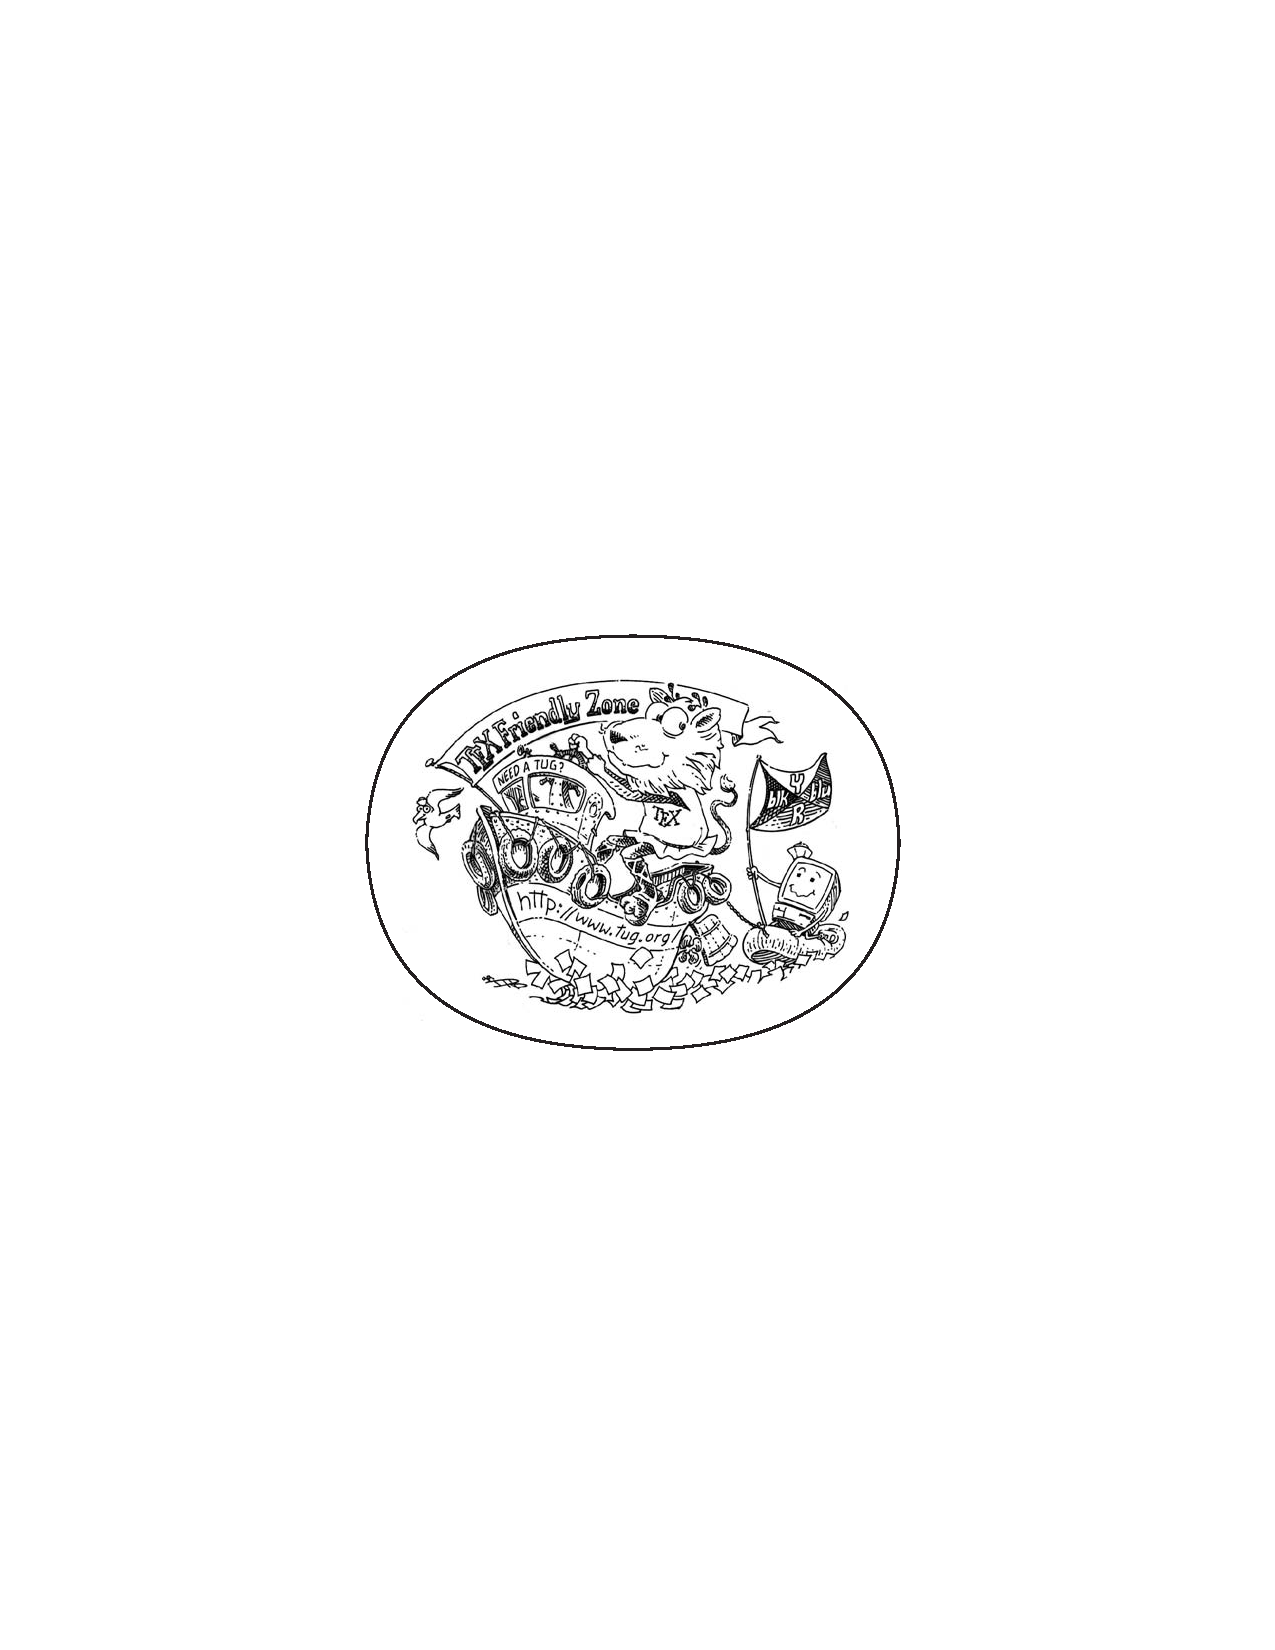
\includegraphics[width=6cm]{gfx/TFZsuperellipse_bw} \\ \medskip

        \mySubtitle \\ \medskip
        %\myDegree \\
        \myDepartment \\
        \myFaculty \\
        \myUni \\ \bigskip

        \myTime\ -- \myVersion

        \vfill

    \end{center}
  \end{addmargin}
\end{titlepage}

\thispagestyle{empty}

\hfill

\vfill

\noindent\myName: \textit{\myTitle,} \mySubtitle, %\myDegree,
\textcopyright\ \myTime

%\bigskip
%
%\noindent\spacedlowsmallcaps{Supervisors}: \\
%\myProf \\
%\myOtherProf \\
%\mySupervisor
%
%\medskip
%
%\noindent\spacedlowsmallcaps{Location}: \\
%\myLocation
%
%\medskip
%
%\noindent\spacedlowsmallcaps{Time Frame}: \\
%\myTime

\cleardoublepage%*******************************************************
% Dedication
%*******************************************************
\thispagestyle{empty}
\phantomsection
\pdfbookmark[1]{Dedication}{Dedication}

\vspace*{3cm}

\begin{center}
      This thing is complex... so complex not even God gets it.\\ \medskip
    --- Rafa Buscalioni
    \\ \medskip\medskip
        There is no way you are getting a quote for your stupid thesis\\ \medskip
    --- NVIDIA

\end{center}

\medskip

%\cleardoublepage\input{FrontBackmatter/Foreword}
\cleardoublepage%*******************************************************
% Abstract
%*******************************************************
%\renewcommand{\abstractname}{Abstract}
\pdfbookmark[1]{Abstract}{Abstract}
% \addcontentsline{toc}{chapter}{\tocEntry{Abstract}}
\begingroup
\let\clearpage\relax
\let\cleardoublepage\relax
\let\cleardoublepage\relax

\chapter*{Abstract}

Some abstract


\cleardoublepage
\pdfbookmark[1]{Publications}{publications}
\chapter*{Publications}

The following publications resulted from the development of this work
%\noindent Put your publications from the thesis here. The packages \texttt{multibib} or \texttt{bibtopic} etc. can be used to handle multiple different bibliographies in your document.

\begin{refsection}[ownpubs]
    \small
    \nocite{*} % is local to to the enclosing refsection
    \printbibliography[heading=none]
\end{refsection}


\cleardoublepage
\pdfbookmark[1]{Acknowledgments}{acknowledgments}

\begin{flushright}{\slshape}
\end{flushright}



\bigskip

\begingroup
\let\cleardoublepage\relax
\let\cleardoublepage\relax
\let\cleardoublepage\relax
\chapter*{Acknowledgments}

Thanks y'all.


\cleardoublepage

\pagestyle{scrheadings}
%\phantomsection
\pdfbookmark[1]{\contentsname}{tableofcontents}
\setcounter{tocdepth}{2} % <-- 2 includes up to subsections in the ToC
\setcounter{secnumdepth}{3} % <-- 3 numbers up to subsubsections
\manualmark
\markboth{\spacedlowsmallcaps{\contentsname}}{\spacedlowsmallcaps{\contentsname}}
\tableofcontents
\automark[section]{chapter}
\renewcommand{\chaptermark}[1]{\markboth{\spacedlowsmallcaps{#1}}{\spacedlowsmallcaps{#1}}}
\renewcommand{\sectionmark}[1]{\markright{\textsc{\thesection}\enspace\spacedlowsmallcaps{#1}}}
%*******************************************************
% List of Figures and of the Tables
%*******************************************************
\cleardoublepage
% \pagestyle{empty} % Uncomment this line if your lists should not have any headlines with section name and page number
\begingroup
    \let\cleardoublepage\relax
    \let\cleardoublepage\relax
    %*******************************************************
    % List of Figures
    %*******************************************************
    \phantomsection
    \addcontentsline{toc}{chapter}{\listfigurename}
    \pdfbookmark[1]{\listfigurename}{lof}
    \listoffigures

    \vspace{8ex}

    %*******************************************************
    % List of Tables
    %*******************************************************
    %\phantomsection
    %\addcontentsline{toc}{chapter}{\listtablename}
    %\pdfbookmark[1]{\listtablename}{lot}
    %\listoftables

   % \vspace{8ex}
    % \newpage

    %*******************************************************
    % List of Listings
    %*******************************************************
    \phantomsection
    \addcontentsline{toc}{chapter}{\lstlistlistingname}
    \pdfbookmark[1]{\lstlistlistingname}{lol}
    \lstlistoflistings

    \vspace{8ex}

    %*******************************************************
    % Acronyms
    %*******************************************************
    %\phantomsection
    \pdfbookmark[1]{Acronyms}{acronyms}
 %   \markboth{\spacedlowsmallcaps{Acronyms}}{\spacedlowsmallcaps{Acronyms}}
%    \chapter*{Acronyms}
    \printglossary[type=\acronymtype]
\endgroup


\cleardoublepage
\pagestyle{scrheadings}
\pagenumbering{arabic}
%\setcounter{page}{90}
% use \cleardoublepage here to avoid problems with pdfbookmark
\cleardoublepage
\part{Introduction}\label{pt:intro}
\chapter{Introduction}\label{ch:introduction}

\begin{figure}[h]
  \centering
  \includesvg[width=\columnwidth]{gfx/scales}
  \caption{The spatio-temporal landscape and its numerical techniques. Different techniques are applied to simulate the different scales invovled in a biological system or, in general, a complex fluid. Zooming in from the bottom-left we have the blood inside a section of a vein, the plasmic environment in a small drop of blood (where cells, platelettes, viruses, etc are present), a virus, a single protein and finally the individual atoms that compose it along the surrounding fluid particles (water).}
  \label{fig:sptime-land}
\end{figure}

The modeling and simulation of physical systems is always tied to a certain spatio-temporal scale. Usually, studying a system through the lens of a certain scale prevents the exploration of the others.
Choosing the right lens for a problem requires understanding its characteristic times and lengths.
Say, for instance, that you want to study the flow of a waterfall throughout the next thousand years. It would be a bad decision to employ quantum mechanics for such a feat, as it is a theoretical framework for events that take femtoseconds and angstroms.

Mathematical frameworks and numerical techniques have been devised for the exploration of different spatio-temporal scales. However, many phisical phenomena are intrinsically \emph{multiscale}, as the effect of small and fast scales affect the larger and slower ones.
The advent of supercomputing in the last two decades has presented the field with new powerful tools to leverage. For the first time we have more computing power than what our techniques are capable of handling. 
Developing new techniques (numerical and theoretical) directly aimed to these new technologies will enable the exploration of regimes previously unreachable, opening the doors to new phenomena.
Multiscale problems will particularly benefit from the improvements in supercomputing.
For instance, \cite{virusfullatom2018} to simulate every molecule of a virus capsid submerged in water ($6$ million atoms) in the span of $1\mu s$ ($5\cdot10^8$ simulation steps).
Another example of these huge simulations, the authors of \cite{fullatombacteria2016} use $100$ million particles to model a chunk of the interior environment of a bacteria for some tens of nanoseconds (around $10^7$ steps).

These sort of simulations would be impossible without the aid of a super computer and specialized software tools to take advantage of it. Indeed, aside from raw computing power, new fast and efficient numerical schemes (adapted to novel computing architectures) are needed to cover larger spatio-temporal windows in physical modeling. This is precisely the objective of this thesis, which is in particular devoted to the development of new algorithms and software tools for the study of complex fluids and biological systems in high performance computing environments.

Most of the properties of complex fluids arise often from an intermediate regime, called the \emph{mesoscale}.
The definition of mesoscale is fuzzy, but normally deals with scales ranging from $50-100nm$ (a typical virus) to $~10\mu m$ (the size of a HeLa cell) (characteristic times go from micro seconds to even minutes).
The mesoscale poses a series of theoretical and numerical challenges, because it stems from the microscopic spatio-temporal scales and yet it interacts with slower processes over large scales. A perfect fit for a super computer.

\todo{continue}

\section{The Graphical Processor Unit}

Recently, a new paradigm of supercomputing has arisen. The \gpu, a massively parallel copocressor. So powerful that it requires to straight-up rethink our algorithms to take advantage of it.

\begin{figure}
  \centering
  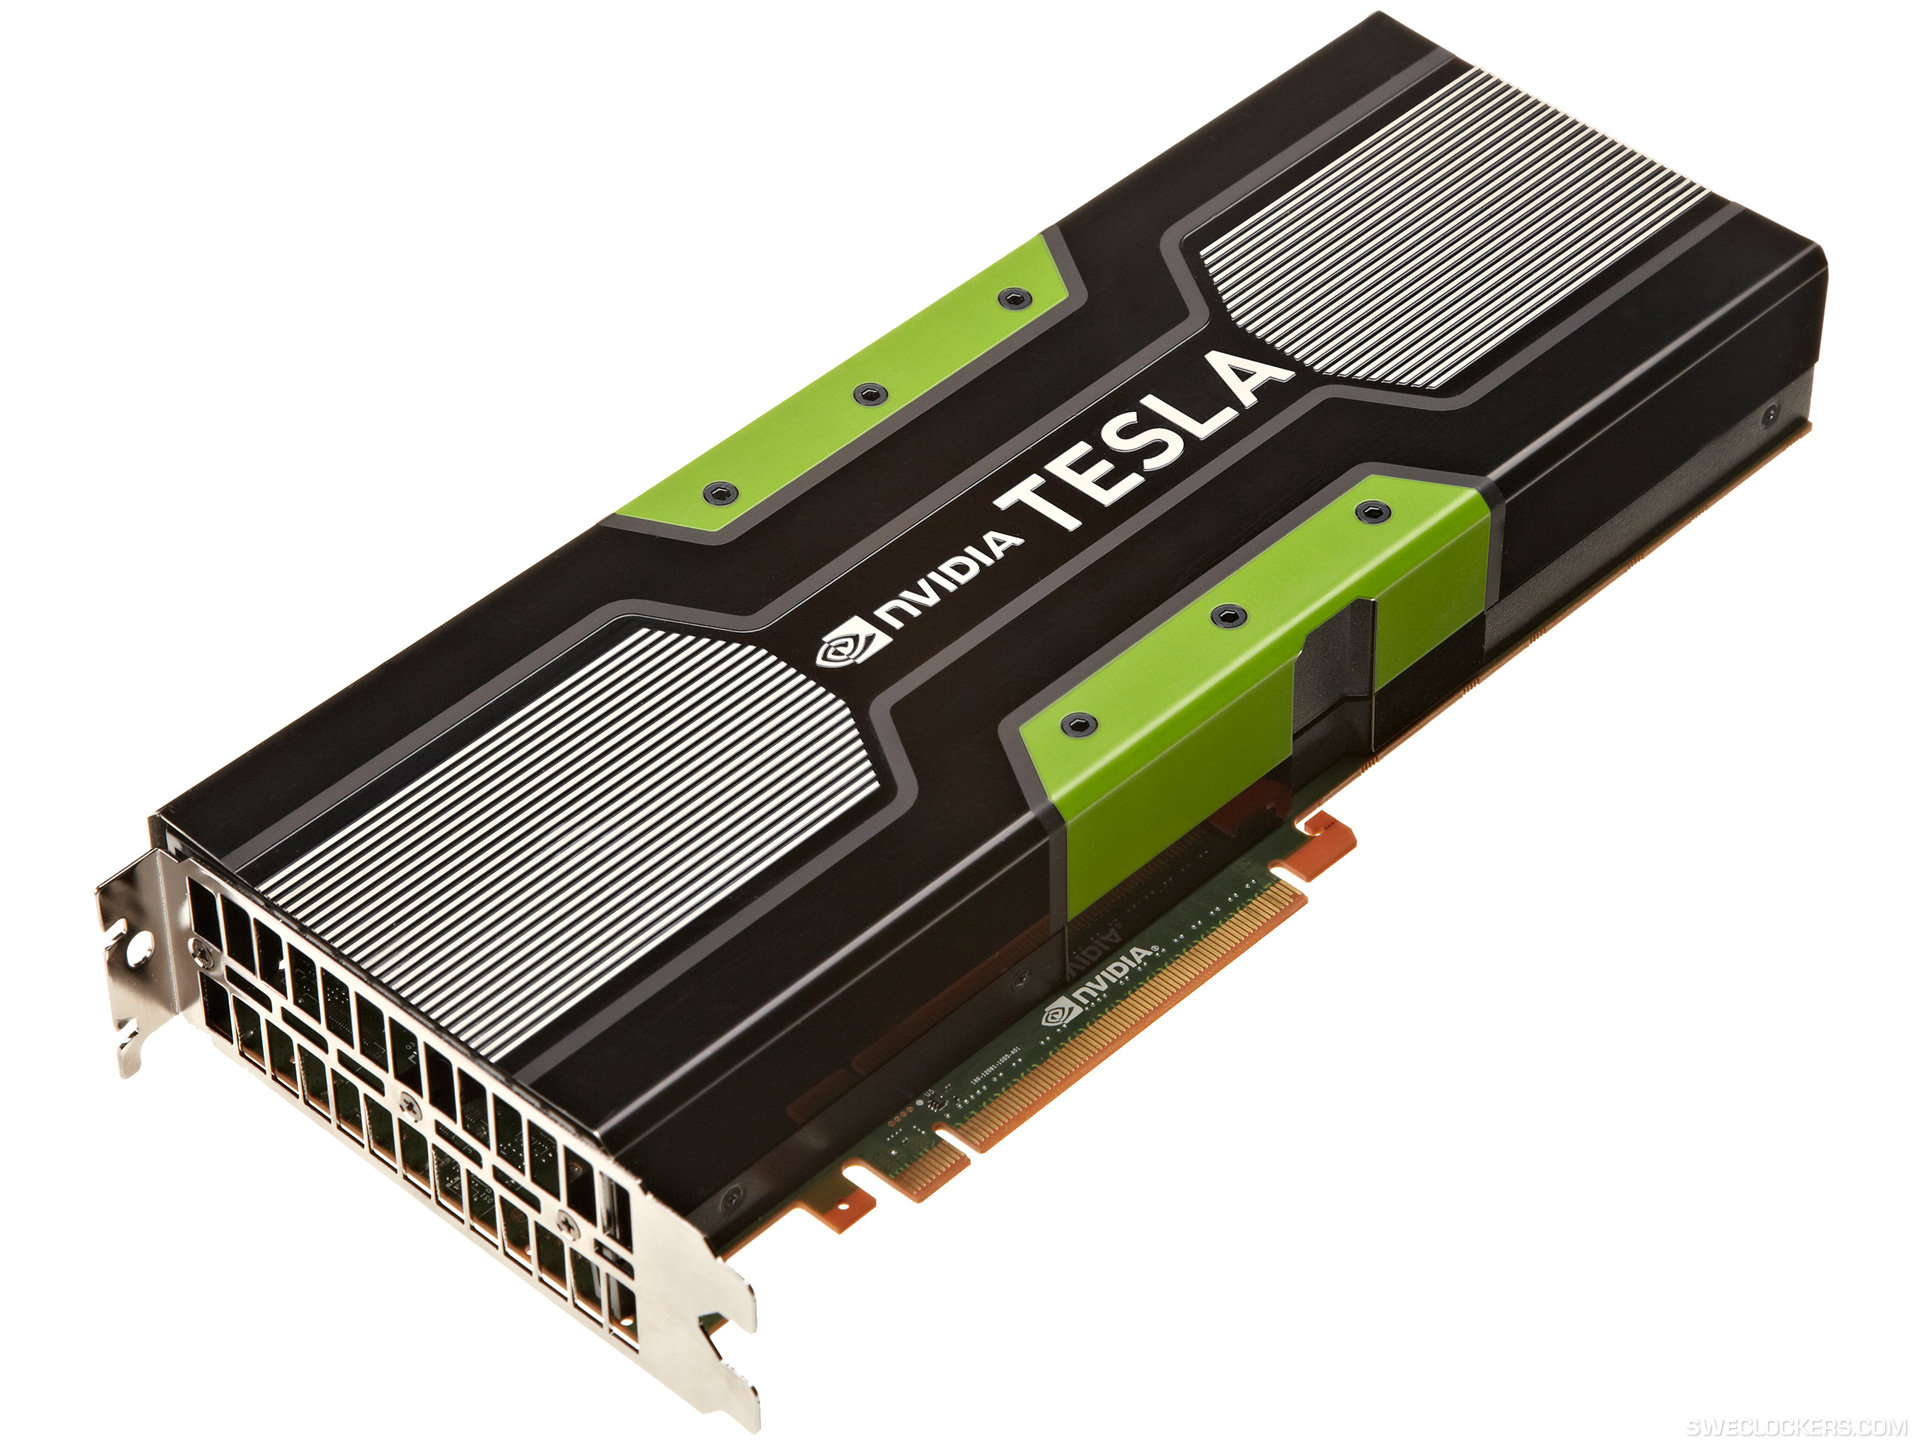
\includegraphics[width=\textwidth]{gpu_and_me}
  \caption{A picture of the author with a GPU (a NVIDIA's RTX 2080Ti). This card will grant its owner the computing power of a small CPU cluster a price of around 1000€.}
  \label{fig:gpuandme}
\end{figure}

Yet, the \gpu technology, interpreted as some kind of specialized graphic circuit or co-processor, can be tracked back to the 1970s. Once electronic devices started having screens attached to them, it made sense to have some kind of chip translating the CPU information into the analogic signal of the display. It was then only a matter of time before more functionality was put into them. It started as a way to accelerate the display process in early video game hardware, such as arcade systems.
Storing the data that goes into the screen takes a lot of space and, at the time, RAM memory was expensive (still is, by the way!).

In 1977, the Atari 2600 (one of the first home consoles) could simply not afford to store the contents of its 160x80 pixel display into its 128 bytes of RAM. Of course, these systems employed some truly creative software tricks to reduce memory usage. However, the numbers just do not add up. Even if we limit ourselves to a monochrome output (so one pixel takes one bit to store), the frame buffer for a 160x80 pixel display takes 1600 bytes\footnote{In contrast, the NVIDIA GTX 980 (the trusty, consumer-grade, GPU that has accompanied my thoughout most of my Ph.D.) has 4 GB of memory and will happily output to a several screens with 4k resolution (4096x2160 pixels).}.
The solution was to not have a frame buffer at all, but rather to outsource the display operations to a specialized hardware. The Atari 2600's graphic chip had a 128 color palette and allowed developers to use close to 5 sprites to design their 2D games.

These chips were little more than video display chips, but they were the predecesors to the \gpu.
Throughout the next decade the hardware evolves to support faster and more complex operations, hold more memory, etc. In 1990 a graphic adaptor could draw 16 million different colors to a 1028x1024 pixel display and hold 1MB of data.

Graphic adaptors were still centered around 2D graphic acceleration, such as graphical user interfaces and 2D games. However, the market was already pushing for real-time 3D graphics in games. Although one could hack the current 2D graphic pipeline to draw 3D environments, without specialized hardware acceleration (as was already common for 2D) the results were far from interactive. Surely it would be a task best suited for the graphic adaptor technology already established.

Soon enough, during the early and mid 1990s, several companies were releasing their graphic adaptors with 3D acceleration capabilities. In 1994 the term \gpu is coined to designate this hardware, which had evolved beyond its original task of just sending pixels to a display.
OpenGL\cite{opengl}, one of the first graphics \gls{API}\footnote{A software library.}, appears in the early 1990s attempting to standardize the programming of graphic hardware accelerators, specially for 3D.
At the time OpenGL had quite limited capabilities, allowing a developer to do little more than to feed a fixed pipeline with triangles. OpenGL would then interface with the \gpu to turn this geometry into a 2D image that could be displayed.
Naturally this translation involves a great deal of raw computation, further transforming the \gpu from a video display card to an independent co-processor. Furthermore the usual operations required to do this happen to be inherently parallel. While the CPU evolved to be formed by a single, powerful, core the \gpu was born out of a parallel computing necessity. Thus a \gpu tends to have many, less powerful, processing cores.
Jumping again to the year 2000 the quality and complexity of computer graphics has exploded. Card manufacturers have included all sorts of new 3D hardware accelerated operations beyond simple triangles. And OpenGL has evolved along them. As it usually happens people have started to hack around, using the graphics pipeline to perform computations not necessarily related to computer graphics. In particular, a new \gpu was presented by the NVIDIA Corporation in 2001 that allowed to modify the different stages of the graphic pipeline via something called programmable shaders. These shaders were short programs that could intercede between the different stages of drawing. A vertex shader could be written to process each triangle before sending it to a fragment shader, which could process each pixel on the screen before finally sending them to the display. This was the advent of the so-called \gls{GPGPU}.

Shaders were enough for the community to realize that drawing polygons was far from the only thing they could do with a \gpu\cite{gpgpu2002}. Applications exploting shaders arise everywhere in a variety fields like scientific image processing \cite{gpuimage2003, gpuimage2006}, lineal algebra \cite{gpulinalg2001, gpulinalg2003a, gpulinalg2003b}, physics \cite{gpulbm2004} and even machine learning\cite{gpuml2005, gpuml1998}. One can even find a molecular dynamics code running on the \gpu of a Sony PlayStation 3 \cite{ps3md2009}.

The next natural step took place in 2007, when the NVIDIA Corporation released CUDA\cite{cuda}\footnote{Although the original accronym for CUDA was Compute Unified Device Architecture, the platform quickly out evolved beyond this definition. However, the term CUDA was already stablished and thus it has remained as the name of the platform.} along its flagship card, the GeForce 8800.

CUDA is programming model and an extension of the C++ programming language that allows to exploit CUDA-enabled \glspl{GPU} for general-purpose computing. It can be considered as a conceptual generalization of the aforementioned graphic shaders that acknowleges the \gpu as a general-purpose processor. Via the inclusion of a small set of keywords and extensions to C++, CUDA exposes the massively parallel architecture of the \gpu under the ecosystem of an already stablished high performance programming language.
Now developers aiming for the \gpu did not have to be experts in hacking a certain graphics \gls{API} and could just focus on parallelizing the algorithms for its particular architecture.

The birth of CUDA became a pivotal moment in high performance computing, opening the doors to a revolution in several fields such as medical analysis, bioinformatics, machine learning, economic market analysis, molecular dynamics and more.

In this thesis, we will push the boundaries of \gpu computing by developing and implementing old and new algorithms for the modelling of soft matter systems into a new infrastructure called \uammd. \uammd is designed from the ground up with the \gpu in mind and is written in CUDA/C++.

One of the main critiques to CUDA is that it is a close sourced, propietary, environment that can only be compiled for NVIDIA's own \glspl{GPU}. This restricts CUDA code to only a subset of \gpu hardware.
In 2009, an open standard called OpenCL\cite{Stone2010} was born (from the creators of OpenGL) as an alternative to CUDA. Although implementations of OpenCL exist for almost any hardware (including GPUs from NVIDIA and AMD, CPUs, FPGAs,...) its adoption has been slow, partly due to an aggressive marketing campaign from NVIDIA to sell CUDA as the better alternative\footnote{Since the birth of CUDA, NVIDIA has been promoting it by donating GPUs to researchers, giving away a plethora of CUDA courses all around the world and more.}. The general sentiment in the community has always been that OpenCL should win as the de facto \gls{GPGPU}-\gls{API} in the long term. However, it simply has not happend yet.
Luckily, there are ways to translate CUDA code into OpenCL code\footnote{In particular, the HIP library works as a thin wrapper over CUDA/OpenCL, allowing to write code that can be compiled for any of the \glspl{API}.} and given that the paradigms of both \glspl{API} are quite similar, it is fairly straight-forward to port CUDA code to OpenCL. Therefore, in the future, porting the software infrastructure presented in this manuscript to OpenCL would be mainly painless and will not require changes to the public \gls{API}. So even though at the time of writing \uammd is restricted to run on NVIDIA's hardware it is possible to adapt it so that it runs on virtually any parallel hardware.


\section{Software for soft matter simulations}

Particle based computer modelling of soft matter systems has been around since the advent of computers. The use of computers for physical simulation can be tracked back as far as to the 1940's when researches at the Los Alamos national laboratory described the use of the ENIAC\footnote{The first programmable, electronic, generalpurpose digital computer.} for simulating some stochastic physical process\cite{Hurd1985} (the origins of the Monte Carlo method\cite{Johansen2010}). Shortly after, in the 1950's, computational molecular dynamics was born\cite{DeTullio2016}.

One of the first examples of a software package for molecular dynamics is CHARMM, whose initial release dates back to 1983\cite{Brooks1983}. To put it in perspective, Windows 1.0 was released in 1985, the UNIX operating system was disclosed to the public in 1973 and Linux originated in 1991. It is humbling to realize that since 1983 the basic layout of a full-fledge molecular dynamics software package has not changed that much. As a matter of fact, the infrastructure presented in this manuscript shares many of the basic conceptual separations already present in \cite{Brooks1983}.

It is important to also mention that MPI, one of the first parallel \glspl{API}, was not available until 1994. Up to that point, sequencial computing was the norm.

Another famous molecular dynamics package is GROMACS, which was released in 1991, with the first version using MPI coming shortly after it's release.


Many of these software packages were born more than a decade before the term \gpu existed and were already quite stablished when the \gpu became a mainstream general purpose computing hardware. Naturally almost all of them have, at least partially, ported their functionalities to be accelerated by a \gpu in some way. However, \gpu programming poses such a wildly orthogonal paradigm that it makes the porting process slow and painful. Most CPU centric molecular dynamics packages are already so complex that redesigning from the ground up to accomodate for the \gpu is not an option and thus their inclusion can become awkward, sometimes causing the so-called software rot.

It is therefore worth it to once in a while start again from a clean slate considering the new environments. One example of this is the general-purpose molecular dynamics software package HOOMD\cite{Anderson2008}. Born around the same time as CUDA itself HOOMD was designed from the ground up with the \gpu in mind. Although HOOMD provides a CPU-only backend it is centered around the \gpu and can work exclusively in it, this is crucial, as communication between the CPU and the \gpu is quite expensive, so much that it can many times negate the benefits of using a \gpu altogether.

Virtually all of the mainstream commercial molecular dynamics packages share one foundational design principle; they are \emph{closed} ecosystems. This means that, for an user, the only option to interface with the packages is to integrate their simulations in them in their totality. In other words, it is awkward (or stright up not possible) to use these packages as external accelerators for an already stablished code. Of course, a closed ecosystem allows to design the software under less assumptions, easing development. On the other hand, a closed ecosystem misses some opportunities in doing so. For instance, one of the first problems a soft matter software package must solve is the construction of a short ranged particle interaction list (a so-called neighbour list), which usually governs the overall computational cost of a simulation. Creating a public, library-like, interface exposing this list creation algorithm allows an user to take his existing code and accelerate it, as opposed to having to do it the other way around, that is porting the entirety of his simulation to the closed ecosystem.

\uammd attempts to provide an \emph{open} ecosystem, exposing most of the underlying algorithms in a library-like fashion.
Furthermore, while most packages require to be compiled into a binary or library in order to be used, \uammd is a header-only framework. Meaning that the compilation of a source code using parts of \uammd can be seamlessly ingrained along the compilation process of another software.


Developing algorithms for the ground up with the GPU architecture in mind is essential. Leverage ultra efficient \gpu \gls{FFT} by developing spectral algorithms. Many times simplicity beats complexity.

State of the art in molecular simulations.
\todo{continue}

\cleardoublepage
\ctparttext{Description of the UAMMD infrastructure. Importance of fundamentally GPU-driven design.}
\part{UAMMD: Design and components}\label{pt:uammd}

\chapter{The Fermation of subproblems}
Consider the development of a software capable of reproducing the dynamics of an ionic solution in a cellular membrane channel. This poses a really convoluted simulation, involving electrostatics, fluctuating hydrodynamics, steric interactions, bonded ligatures, etcetera\footnote{A simulation easily handled by \uammd, by the way.}. As we will see along this manuscript, some of these algorithms are quite complex on their own, depending on a lot of moving parts. The mathematical and theoretical machinery required to model something like that appears to be in the realm of a theory of everything. It surely seems like an intractable feat!.
We could try to design, from the ground up, a software that can perform this hypothetical simulation. While quite restricted to the specific usecase, the result would even be somewhat flexible. For instance, we could turn off electrostatics by setting the charges of all particles to zero.

However, this top-down approach is fundamentally flawed, we are trying to build the house starting by the roof and losing sight of the forest in the process. The final product will probably have a lot of internal dependencies, many of which are probably unnecesary. In software this means that the code will be hard to adapt or extend.

We humans are not good with complex things (which is probably the reason why complex and complicated share the same ethimology) and, as it can be glimpsed throughout \uammd, my solution to this problem is often to remove the problem altogether.

This approach starts by dividing the original problem into subproblems in a hierarchical fashion (see fig. \ref{fig:uammdsketch}). The top of the tree represents the most general (or abstract) aspect of the problem, and subdivisions offer increasingly specific concepts. So instead of designing our framework with an ionic solution in a membrane channel in mind, we start at the top and then hierarchically specialize. What constitutes the ``top'', or \emph{soul}, of the problem is of course highly subjective and thus the contents of the next sections should be considered but merely my humble take on it.

In particular, we can find the root by removing assumptions until we get to a point where only one (or a small number of them) remains. Therefore, we do not design in terms of ``ions'', ``cells'' or ``molecules'', rather in terms of a vague concept called ``particles''.

Of course, this is not an original idea, coming, in part, from the underlying mindset of the famous Fermi estimates by embracing the (redundant) complexity of complex fluids instead of trying to fight it.

The \uammd framework takes this KISS\footnote{Keep It Simple, Sir} philosophy very seriously. It is supported on a handful of (deliberately) vague assumptions which can be summarize in four:
\begin{enumerate}[label=\textbf{S.\arabic*}]
\item The \emph{System} assumption: The code will run primarily on a \gpu (the most limiting assumption).
\item The \emph{ParticleData} assumption: Simulations are based on the state of ``particles'' (whatever a particle and it's state mean).
\item The \emph{Integrator} assumption: The state of these particles changes in time.
\item The \emph{Interactor} assumption: Particles can interact between them and with an external influence.
\end{enumerate}
These are the four pilars depicted in fig. \ref{fig:uammdsketch}. The software framework exposes these assumptions through four foundational classes (i.e objects in programming), which are, in order; \emph{System}, \emph{ParticleData}, \emph{Integrator} and \emph{Interactor}.

\begin{figure}[h]
  \centering
  \includesvg[width=\columnwidth]{gfx/sketchUAMMD}
  \caption{The basic hierarchy of concepts (and code) in \uammd, represented by a series of modules connected by arrows that convey the direction of the data flow. \emph{System} holds information about the actual physical hardware, and all the entities below rely on it to interact with the environment. \emph{ParticleData} (a ``real class'' in the code) stores all the information about the particles in the simulation, such as positions ($\vec{r}$), velocities ($\vec{v}$), mass, etc, as well as other properties like the current forces acting on it ($\vec{F}$), energy ($E$) or virial ($T$). Modules below (explained later) can request, at their leisure, a list with any of the particles properties. \emph{Integrators} and \emph{Interactors} are interfaces (called virtual classes in programming terms), are in charge of, respectively, forwarding the simulation one step in time and computing the forces, energies and/or virials acting on each particle. These ``Interfaces'' (drawn in red) are abstract objects that cannot be instanced on their own but rather must be inherited. For instance, Brownian Dynamics (section. \ref{sec:bd}) would be an \emph{Integrator}, while a module that computes gravitational forces would be an \emph{Interactor}.}
  \label{fig:uammdsketch}
\end{figure}
\todo{Add something about gpu arch in System in the fig, gpu arch, ncores,...}
Excluding the first assumption, which is unrelated to physics, it is straight forward to see that our initial ionic solution simulation fits in this criteria. As a bonus, we have ended up with a basis that also describes things like ``a gas of argon atoms'', ``a group of planets orbiting a star'' or ``a virus filled with proteins exploding due to the force exerted on it by an AFM tip''\footnote{An oddly specific example describing a real study that is being carried out with \uammd at the moment of writing by a collaborator group.}.

At the top of the tree in fig. \ref{fig:uammdsketch} we find the \emph{System} object which takes care of setting up the computational environment for the rest of players. We discuss \emph{System} in mode detail in sec. \ref{sec:system}.

The second assumption is represented in the code base via the \emph{ParticleData} object, which we discuss in \ref{sec:dynmol}.

Then, we can focus on each of the last two asumptions and apply this separation again. For instance, instead of grouping all interactions (fourth assumption) into a single entity (class) that deals with all possible interactions, we can split the concept between general things like short ranged, bonded or long ranged interactions. In section \ref{sec:interactions} we explore deeper along the \emph{Interactor} branch to discuss the different algorithms and programming interfaces related with particle interactions (see fig. \ref{fig:uammdsketch_interactors}.

Similarly, in section \ref{sec:dynamics} we break down the \emph{Integrator} branch (bottom left of fig. \ref{fig:uammdsketch}) into the several ways the state of the particles can evolve (see fig. \ref{fig:uammdsketch_integrators}).

During the following chapters, we will discuss in detail this conceptual and programmatic hierarchy and follow its branches down to the leaves. This ``final'' computational objects representing the leaves of \uammd encapsulate the actual algorithms and physics in the form of isolated, individual modules. A ``module'' can be understood as a piece of code which recieves information, processes it, and send back some output. The internal complexity of a module is usually much larger than that related with its input and output. Input and output are the essence of the communication between modules.

In general, these modules will communicate only via the closed loop described by \emph{ParticleData}-\emph{Integrator}-\emph{Interactor} in fig. \ref{fig:uammdsketch}.

One of the main unwritten lessons we will glimpse is that it is never a good idea to introduce dependencies that climb up through the tree. Just to give some examples of this:
\begin{itemize}
\item A neighbour list should not assume it is going to be used to
  compute the forces of a group of repulsive particles.
\item The existence
  of an hydrodynamics integrator module should not incur in the
  modification of the \emph{Integrator} interface.
\end{itemize}
In other words, conceptual complexity and problem specificity should increase only downwards through the tree. This forces us as developers to modify a certain module only to generalize it, and never to especialize it. If a module appears to require being especialized, it is almost always a sign that either it should be actually generalized or exist as a separate entity beneath the initial one. This is what makes \uammd so modular and extensible. See figures \ref{fig:uammdsketch_interactors} or \ref{fig:uammdsketch_integrators}, the next lower branches.

\uammd carefully avoids these kind of inter-dependencies.

\chapter{It's in the name}\label{ch:design}

It is common knowledge that a good software starts with a good acronym. \uammd stands for Universally Adaptable Multiscale Molecular Dynamics in an attempt to abridge the simple-yet-powerful four assumptions in the previous chapter\footnote{Naturally, the fact that the acronym for the Universidad Autonoma de Madrid is there is merely a coincidence}. Each of the words carries a different aspect of the framework's philosophy. In this chapter, we will discuss each of them.
\section{Universality}

Complex fluids are one of the prime examples of a multiphysics system. As such, multiphysics are deeply ingrained part of \uammd. Our framework can potentially take into account physical phenomena emerging from fields like electrostatics, thermodynamics, hydrodynamics and more.

One of the key features for \emph{universality} is to be able to communicate between Eulerian (fields) and Lagrangian (``particles'') descriptions. This hybrid approach permits \uammd to efficiently solve problems involving hydrodynamics, electrostatics, magnetism, light-matter interactions, and more... 
  
%Although we focus on the dynamics of particles, which have a Lagrangian description, using an intermediate Eulerian description is a possibility in these situations.
In chapter \ref{sec:bdhi}, we will describe a series of Eulerian-Lagrangian algorithms that incorporate the effect of a solvent in a group of submerged particles (hydrodynamics) by describing it explicitly. On the other hand, we will adapt these techniques to compute electrostatics in chapter \ref{ch:tppoisson} by describing an explicit \emph{charge-density field}.

Quantum physics have not been mentioned yet and for the time being we have limited our toolset to the classical world. Thus, staying in the realm of classical physics could be consider a fifth (soft) assumption.

It is however importatn to stress that the central (class) object in \uammd are the particles (see below). In fact, the fourth assumption in chapter \ref{pt:uammd} states that particles are expected to interact between them or via an external influence. When particles are submerged in a fluid, its effect on the former can be considered an external influence. Even when the fluid itself is also affected by the presence particles, as is the case with hydrodynamics.

\section{Adaptability}


\begin{figure}[h]
  \centering
  %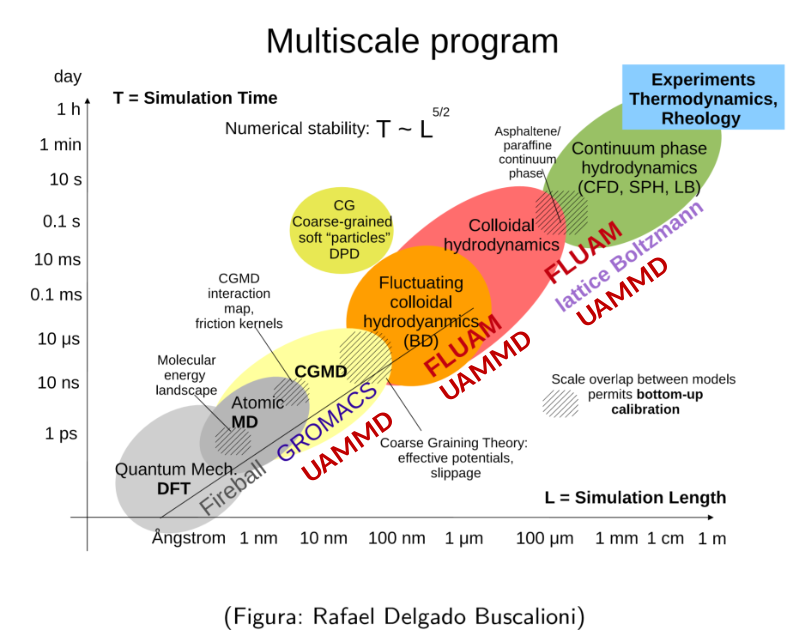
\includegraphics[width=\textwidth]{landscape}
  %\includesvg[width=0.8\columnwidth]{gfx/modular}
  \includesvg[width=0.8\columnwidth]{gfx/virus}
  \caption{A simulation is constructed by putting together several modules. In this instance, the simulation of a virus submerged in water could be constructed by joining an hydrodynamics \emph{Integrator} module with several \emph{Interactors} describing the interactions between particles, such as sterics, bonds, electrostatics,...}
  \label{fig:modular}
\end{figure}

Modularity is another central philosophy in \uammd, which provides it's adaptability. 

Even when the internal complexity of each separate module can be quite great it never bleeds into the rest of the modules, which can remain oblivious to each other. This allows each module to only worry about solving one specific problem (hydrodynamics, electrostatics,...).

On the other hand, this makes \uammd extremely adaptable, since new modules can be added without disturbing the ecosystem.

In \uammd a simulation is described by connecting a series of \emph{Integrators} with an \emph{Integrator}. In fig. \ref{fig:modular} we can see an example of a simulation which connects a hydrodynamics \emph{Integrator} (such as the ones described in sec. \ref{sec:bdhi}) is connected with an \emph{Interactor} that deals with sterics (see sec. \ref{sec:shortrange}), another one that computes electrostatics (see sec. \ref{ch:tppoisson}), and so on and so forth. The communication between these modules is minimal, being mostly restricted to the closed loop in fig. \ref{fig:uammdsketch}. Although nothing prevents two \emph{Interactors} from explicitly sharing information, this never happens in \uammd. 


This does not imply that each module should exist in a completely isolated environment, since a plethora of utilities are available in \uammd to aid with the typical problems that arise in complex fluids. For instace, a module in need of a neighbour list does not need to write one, rather can simply make use of one of the already implemented ones (see chapter \ref{sec:nlist}).

Adaptability also means that, when it makes sense, a module can be specialized from the outside. For instance, the \emph{Interactor} module that computes bonded forces (particles joined by springs or similar ligatures) is not specific to a particular potential. As users, we can specialize it, via the use of C++ templates, to work with a harmonic\cite{harmonic}, FENE\cite{fene}, Morse\cite{morse}, or an arbitrarily complex potential.

The use of metaprogramming (in the C++ sense) reaches every corner of the code base, in many cases allowing to customize (or hack) an utility or module beyond its intended scope without having to modify a single line of it.

\uammd is presented as a CUDA/C++ header-only library and it is mostly self-contained in terms of dependencies. The use of the word library is not chosen lightly here. We have discussed how an \emph{Integrator} is joined with a collection of \emph{Interactors}, maybe suggesting that the latter cannot function without the former. This is not the case since our framework provides a completely open ecosystem, facilitating (and actually encouraging) the incorporation of \uammd modules outside their \emph{normal} environment.
All the utilities in \uammd, including \emph{Interactors}, \emph{Integrators}, neighbour lists, linear solvers and many more\footnote{A list of all the modules in \uammd at the time of writing can be found in Appendix \ref{sec:modulelist}.} \todo{Maybe include here an actual list of things like nlists, ibm, fft, bvp solver,... it is quite the long list...} can be used in an isolated way from ouside the code base. This also means that parts of \uammd can be used as accelerators in already stablished codes. For instance, an already written simulation code can include one of our fast \gpu hydrodynamics implementations into their description with just a few lines of code.

In the past, we have explored this facet of the project by providing to collaborators some of our utilities and solvers as stand alone Python interfaces.

The modularity of \uammd is reflected directly in the code, where modules can be created independently of each other as in the example code \ref{code:module}.
Be it an \emph{Integrator} (hydrodynamics, molecular dynamics,...) or \emph{Interactor} (short range, bonded,...), all modules in \uammd can be created and stored individually.
%The \emph{ParticleData} object here, which is the direct expression in code of the second assumption, will be described in detail in sec. \ref{sec:particledata}.
\todo{Maybe switch the order of the code examples here. In fact, join them both and say that the preamble is going to be omited. Take both code examples below ParticleData. Specify ``Module'' is an Integrator or an Interactor.}
\section{Multiscale}
\begin{figure}[h]
  \centering
  \includesvg[width=\columnwidth]{gfx/landscape}
  \caption{The spatio-temporal landscape and its numerical techniques. Different techniques are applied to simulate the different scales invovled in a biological system or, in general, a complex fluid. Image courtesy of Rafael Delgado-Buscalioni.}
  \label{fig:landscape}
\end{figure}
\begin{figure}[h]
  \centering
  \includesvg[width=0.7\columnwidth]{gfx/multiscale}
  \caption{The different levels of coarse grained description available in \uammd for soft matter simulations.}
  \label{fig:multiscale}
\end{figure}

Describing a given system in a reductionist manner, by solving the dynamics of every atom involved, is of course unfeasible. The \uammd infrastructure can accomodate for several levels of description by making use of coarse graning techniques. Coarse graining allows to realistically describe a system using fewer degrees of freedom.
In general, a level of description is tied to a certain time scale and is characterized by series of relevant variables coupled via a (usually stochastic) dynamic equation.

Although \uammd is not restricted to it, this work is mainly devoted to the study of soft matter systems. In this regard we can identify a series of clearly separated levels of description. It is worth to summarize them here since during this manuscript many of them will be discussed in detail and are furthermore available as \uammd \emph{Integrator} modules. A representation of the different levels of description is available in fig. \ref{fig:multiscale}, while the numerical methods employed to numerically study each of them can be seen in fig. \ref{fig:sptime-land}. Figure \ref{fig:landscape} provides an overview of the different fields of soft matter simulation and its characteristic spatio-temporal scales. We can distinguish between the following levels of description (from most to least detailed):
\begin{enumerate}
\item Microscopic: The relevant variables are the positions and moments of every particle in the system, including the solvent and solute particles. This level is dominated by the mean collision time between the particles, in the order of $\tau \sim 10^{-12} s$. The (purely Lagrangian) Newton equations of motion describe the dynamics of the system and \gls{MD} can be used to solve them. We explore this description in chapter \ref{sec:md}.
\item Hydrodynamic: The degrees of freedom of the solvent particles are omitted and turned into hydrodynamic fields. The Newton equations for the solute particles are coupled with the (fluctuating) Navier-Stokes equations that describe the solvent in what constitutes an Eulerian-Langrangian description. An infinitesimal region of space represents a group of solvent particles, whose individual degrees of freedom are lost. The characteristic time is now controlled by the speed of sound of the solvent ($\tau \sim 10^{-9}s$) and the vorticity ($\tau \sim 10^{-6}s$). We study the hydrodynamic level in chapter \ref{sec:bdhi}.
\item Langevin: Particles move so slowly compared to the solvent characteristic times that hydrodynamic interactions are effectively instantaneous. Only the positions and momentum of the particles remain as relevant variables (Lagrangian description once again), which are described by a Langevin equation. The characteristic decorrelation time of the particle's velocities governs this scale with $\tau\sim 10^{-5}s$. We explore this inertial level of detail in chapter \ref{sec:langevin}.
\item Smoluchowski: Particle positions change slowly enough that their velocity decorrelates effectively instantenously, inertia can be disregarded and positions are the only relevant variable. The dynamics are described by the \gls{BD} equations of motion (an overdamped Langevin equation). The diffusion time of the particles, $\tau \sim 10^{-3} s$, dominates this level. We study this limit in chapter \ref{sec:bd}.
\end{enumerate}
Above these levels of description particles are no longer relevant. Here we have the Fick level, in which a continuum particle concentration field is the relevant variable, and the thermodynamic level, in which the relevant variables are the macroscopic dynamical invariants of the system (mass, energy, volume, temperature,...). We can use these descriptions to study time scales of seconds (Fick) up to infinity (thermodynamics). However, given that \uammd is a particle-centric framework, these descriptions will not be considered in this manuscript.


With the exception of the microscopic level, in which particles experience effective interactions that come directly from quantum effects, every other level emerges as a coarse grained description of the previous one. 

Going from one level to the next incurs losing information (AKA degrees of freedom, e.g the hydrodynamic level cannot track the positions/momenta of the microscopic solvent particles). These eliminated, fast, degrees of freedom are modeled (reintroduced) as a drag coupled with thermal noise. In the following sections, we will see how dissipation is intimately related with thermal noise via the fluctuation-dissipation theorem, such relations ensure that the coarse-grained system attains the correct equilibrium distribution.


\subsection{The Fokker-Planck Formalism}\label{sec:fpe}
One of the basic theories for coarse graining is embeded in the Fokker-Planck formalism. Let us focus on a certain relevant slow, degree of freedom (variable) that interacts, in a \emph{random} way, with many other, fast, degrees of freedom. In general, we will eliminate fast variables from our description and reintroduce them as fluctuations. The \gls{FPE} describes the evolution of the probability distribution, $P(\vec{x},t)$, of a set of relevant or slow variables, $\vec{x} = \{x_1, x_2,\dots, x_N\}$ in a quite general way:
  \begin{equation}
    \label{eq:fpe}
    \partial_t P = -\vec{\partial}_{\vec{x}}\cdot \vec{J}
  \end{equation}
Where $P_0 := P(\vec{x}_0, t_0)$ is known and $\vec{\partial}_{\vec{x}}\cdot \vec{J} := \nabla_{\vec{x}}\cdot\vec{J} = \sum_i\partial J_i/\partial_{x_i}  $ represents the divergence (note that the derivation is made with respect to the slow variables in general vectors\todo{What does this mean??}).
The probability flux vector, $\vec{J}$ is defined as
\begin{equation}
  \label{eq:fpeflux}
  \vec{J}(\vec{x}, t) := \vec{D}^{(1)}(\vec{x},t)P - \tens{D}^{(2)}(\vec{x}, t) \vec{\partial}_{\vec{x}}\cdot P
\end{equation}
The first term is called the drift or transport term (being $\vec{D}^{(1)}$ the drift coefficients) and the second one the diffusion term (being $\tens{D}^{(2)}$ the diffusion coefficients). The \gls{FPE} \eqref{eq:fpe} is written in the so-called ``kinetic form'' and comes from truncating the Kramers-Moyal equation at the second term (via the Pawula theorem)\cite{Risken2012}.

%It is useful to write eq. \eqref{eq:fpeflux} in its kinetic form
%\begin{equation}
%  \label{eq:fpeflux}
%  \vec{J} = \widetilde{\vec{D}}^{(1)}P - \tens{D}^{(2)}\vec{\partial}_{\vec{x}} P
%\end{equation}
%By redefining the drift term as $\widetilde{\vec{D}}^{(1)} := \vec{D}^{(1)} - \vec{\partial}_{\vec{x}}\cdot\tens{D}^{(2)}$.
%
The \gls{FPE} in eq. \eqref{eq:fpe} simply represents the conservation of the conditional probability $P(\vec{x},t)d\vec{x}$ of finding a set of variables $\vec{x}$ in the range $[\vec{x}, \vec{x} + d\vec{x}]$. The generality of eq. \eqref{eq:fpe} makes it applicable in a wide range of situations (a suspension of colloidal particles, fluctuations in electrical circuits, mechanical oscillators and chemical reactions just to name a few).

We can use the probability distribution $P$ to compute the the average of a certain function $f(\vec{x}(t))$

\begin{equation}
  \left\langle f\right\rangle(t) = \int {P(\vec{x},t) f(\vec{x}) d\vec{x}}.
\end{equation}
Its time evolution can be then expressed as
\begin{equation}
  \begin{aligned}
    \frac{d\left\langle f\right\rangle}{dt} &= \int{f\partial_tPd\vec{x}}\\
    &= \left\langle \vec{D}^{(1)} \vec{\partial}_{\vec{x}}f\right\rangle + \left\langle \tens{D}^{(2)}\vec\partial_{\vec{x}}^2f\right\rangle.
  \end{aligned}
\end{equation}
The choice of names for the coefficients becomes evident if we now study the first moments of the relevant variables. The first one (the mean) yields
\begin{equation}
  \label{eq:fpemean}  
  \frac{d\langle\vec{x}\rangle}{dt} = \underbrace{\left\langle \widetilde{\vec{D}}^{(1)}\right\rangle}_{\text{Drift}} = \overbrace{\left\langle \vec{D}^{(1)}\right\rangle}^{\text{Systematic drift}} + \underbrace{\left\langle \vec{\partial}_{\vec{x}}\cdot\tens{D}^{(2)}\right\rangle}_{\text{Thermal drift}}
\end{equation}
Where $\widetilde{\vec{D}}^{(1)} := \vec{D}^{(1)} + \vec{\partial}_{\vec{x}}\cdot\tens{D}^{(2)}$.
In the next section, we will see that the second moment, the variance of the relevant variables, is closely related with the diffusion coefficients, $\tens{D}^{(2)}$. It is however straight-forward to study the variance in the case of a single dimension with a variable $x$, where the variance can be written as
\begin{equation}
  \label{eq:fpevar}
  \frac{d\langle x^2\rangle}{dt} = \left\langle 2 D^{(1)}x\right\rangle + 2\underbrace{\left\langle D^{(2)}\right\rangle}_{\text{Diffusion}}.
\end{equation}

In section \ref{sec:langevin} we will study the Langevin equation, a case in which the relevant variables are the velocities (and positions) of the particles (which are surrounded by a bath of fast moving water molecules). On the other hand, in section \ref{sec:bd} we will see that in Brownian Dynamics (the overdamped limit of the Langevin equation), the relevant variables are the positions of the particles (being their velocities the fast, eliminated, degree of freedom). Finally, the applicability of the Fokker-Planck formalism at the hydrodynamic level will be briefly discussed in chapter \ref{sec:bdhi}.

\subsection{Fluctuation-Dissipation balance}\label{sec:fdb}
A system in contact with a heat bath will exprience both friction and fluctuations stemming from the elimination of a series of fast degrees-of-freedom. Both magnitudes are directly related to each other in equilibrium, as the equipartition theorem states that every degree-of-freedom has $\kT/2$ kinetic energy, which requires that fluctuation and dissipation are in a certain specific balance.

We will see what the \gls{FPE} tells us about the fluctuation-dissipation balance by studying the covariance matrix,
\begin{equation}
\tens{\sigma} :=\left\langle \delta\vec{x}\otimes\delta\vec{x}\right\rangle,
\end{equation}
of the relevant variables. Here $\otimes$ represents the tensor product and $\delta\vec{x} = \vec{x} - \langle\vec{x}\rangle_{\text{eq}}$ is a fluctuation of the relevant variables around their equilibrium averages.

Let us also define the transport coefficients as fluctuations around their equilibrium mean, such that and $\delta\vec{D} := \vec{D} - \langle\vec{D}\rangle_{\text{eq}}$.
Using eqs. \eqref{eq:fpemean} and \eqref{eq:fpevar}, it can be shown that the time evolution of the covariance is then given by
%\begin{equation}
%  \label{eq:fpesigma}
%  \partial_t\tens{\sigma} = 2\left\langle\tens{D}^{(2)} \right\rangle + \left\langle \vec{x}\otimes\vec{D}^{(1)} \right\rangle - \left\langle \vec{x} \right\rangle\otimes\left\langle \vec{D}^{(1)}\right\rangle
%\end{equation}
%This allows to rewrite eq. \eqref{eq:fpesigma} as  %, where  $\bar{\vec{x}} := \langle \vec{x} \rangle$.
\begin{equation}
  \label{eq:fpefdsigma}
 \partial_t\tens{\sigma} = 2\left\langle\tens{D}^{(2)} \right\rangle + \left\langle \delta\vec{x}\otimes\delta\vec{D}^{(1)} \right\rangle + \left\langle \delta\vec{D}^{(1)}\otimes\delta\vec{x} \right\rangle.
\end{equation}
For convenience, let us define $\bar{\vec{x}}:=\left\langle\vec{x}\right\rangle_{\text{eq}}$.
The transport coefficients can then be decomposed as
\begin{equation}
  \label{eq:fpefdcoeff}
  \vec{D}^{(i)}(\vec{x}, t) = \vec{D}^{(i)}(\bar{\vec{x}}, t) + \left.\vec{\partial}_{\vec{x}}\vec{D}^{(i)}\right|_{\text{eq}}\delta\vec{x}+\dots
\end{equation}
Where $i$ can refer to the drift or diffusion coefficients.
Eq. \eqref{eq:fpefdcoeff} allows to approximate
\begin{equation}
  \delta\vec{D}^{(1)} = \left.\vec{\partial}_{\vec{x}}\vec{D}^{(1)}\right|_{\text{eq}}\delta\vec{x} + O\left(\delta\vec{x}^2\right)
\end{equation}
Let us now define the dynamic matrix, $\tens{H}$ as
\begin{equation}
  \tens{H} := -\vec{\partial}_{\vec{x}}\vec{D}^{(1)}(\bar{\vec{x}},t)
\end{equation}
So that
\begin{equation}
  \label{eq:fpefdhd}
  \delta\vec{x}\otimes\delta\vec{D}^{(1)} = -\tens{H}\left(\delta\vec{x}\otimes\delta\vec{x}\right) + O\left(\delta\vec{x}^3\right)
\end{equation}
In a stationary or equilibrium state we have $\partial_t\tens{\sigma} = 0$. Replacing eq. \eqref{eq:fpefdhd} into \eqref{eq:fpefdsigma} in equilibrium yields
\begin{equation}
  \label{eq:fpefdbal}
  2\left\langle\tens{D}^{(2)}\right\rangle = \tens{H}\tens{\sigma}_{\text{eq}} + \tens{\sigma}_{\text{eq}}\tens{H}^T
\end{equation}
This key relation is known as the Fluctuation-Dissipation Balance.

We can now go a little bit further and investigate the evolution of the relevant variables during a small time internal, $dt$, which will allow us to derive an \gls{SDE}.
Let us assume that we know the values of the relevant variables at some initial point in time, $t_0 = 0$, so that $P(\vec{x}, t_0) = \delta(\vec{x}-\vec{x}_0)$ (where $\vec{x}_0 :=\vec{x}(t_0)$).

If the time interval is small enough, we can safely assume that the transport coefficients remain mostly constant ($\left\langle\vec{D}^{(i)}(\vec{x}) \right\rangle = \vec{D}^{(i)}(\vec{x}_0)$). Furthermore, we can neglect any terms beyond $dt$. 
Making use of the definition of derivative, we can now write eqs. \eqref{eq:fpefdsigma} and \eqref{eq:fpemean} as

\begin{align}
    \left\langle\vec{x}\right\rangle(dt) &= \vec{x}_0 + \vec{D}^{(1)}(\vec{x}_0)dt\label{eq:fpesdemean}\\
    \tens{\sigma}(dt) &= \left\langle \delta\vec{x}\otimes\delta\vec{x}\right\rangle = 2\tens{D}^{(2)}(\vec{x}_0)dt + O(dt^2)\label{eq:fpesdefluc}
\end{align}

Note that $\tens{\sigma}(t_0) = 0$ since que know $\vec{x}_0$ exactly. Finally, we can decompose any function into its average and a fluctuation, so that $\vec{x} = \left\langle\vec{x}\right\rangle + \delta\vec{x}$. We can then write an \gls{SDE} for the relevant variables
\begin{equation}
  \label{eq:fpesde}
  d\vec{x} = \vec{x}(dt) - \vec{x}_0 = \vec{D}^{(1)}dt + \delta\vec{x}
\end{equation}
Where the fluctuating part must satisfy eq. \eqref{eq:fpesdefluc}. Furthermore, the diffusion and drag terms are related via the fluctuation-dissipation balance in eq. \eqref{eq:fpefdbal}.

In future chapters, we will apply the Fokker-Planck formalism to the different levels of detail described in fig. \ref{fig:multiscale} and its related discussion.

\subsection{Einstein relation}\label{sec:einstein}
An extremely important relation between transport coefficients appearing in $\vec{D}^{(1)}$ and the diffusion $\tens{D}^{(2)}$ can be derived from the equilibrium state, $\vec{J} = 0$ in eq. \eqref{eq:fpeflux}. This relation was first defined by Einstein\cite{EinsteinRelation} with arguments similar to those exposed in what follows.

Consider the zero flux condition $\vec{J}=0$, which is solved by the equilibrium distribution $P_{\text{eq}}(\vec{x})$ (independent on time)
\begin{equation}
  \label{eq:fluxeq}
  \vec{J} = \vec{D}^{(1)}P_{\text{eq}} - \tens{D}^{(2)}\vec{\partial}_{\vec{x}}P_{\text{eq}} = 0
\end{equation}
Thus
\begin{equation}
  \label{eq:fluxeqln}
\vec{\partial}_{\vec{x}}\ln \left(P_{\text{eq}}\right) = \frac{\vec{D}^{(1)}(\vec{x})}{\tens{D}^{(2)}(\vec{x})}
\end{equation}
Now, quite generally, consider that $\vec{D}^{(1)} = -\tens{M}\vec{\partial}_{\vec{x}}U(\vec{x})$ where $U$ is the free energy of the system, satisfying $P_{\text{eq}} = \frac{1}{Z}\exp\left[-\beta U(\vec{x})\right]$ (or $\vec{\partial}_{\vec{x}}P_{\text{eq}} = -\beta \vec{\partial}_{\vec{x}} U(\vec{x})$) and $\tens{M}(\vec{x})$ is called ``mobility'', as it relates forces ,$\vec{F} = -\vec{\partial}_{\vec{x}}U$, with the displacement created by the systematic drift, $\left\langle d\vec{x}\right\rangle = \tens{M}\vec{F} dt$. Inserting $\vec{D}^{(1)} = -\tens{M}\vec{\partial}_{\vec{x}}U$ into eq. \eqref{eq:fluxeqln} and comparing with the equilibrium result, we conclude that
\begin{equation}
  \frac{\vec{D}^{(1)}(\vec{x})}{\tens{D}^{(2)}(\vec{x})} = \frac{-\tens{M}(\vec{x})\vec{\partial}_{\vec{x}}U}{\tens{D}^{(2)}(\vec{x})} = -\beta\vec{\partial}_{\vec{x}}U
\end{equation}
So that,
\begin{equation}
  \label{eq:einsteinrel}
  \tens{M}(\vec{x}) = \beta\tens{D}^{(2)}(\vec{x})\quad\text{ or }\quad\tens{D}^{(2)}(\vec{x}) = \kT\tens{M}(\vec{x})
\end{equation}
Which is the celebrated Einstein relation. Note that the Einstein relation also relates fluctuations (governed by $\tens{D}^{(2)}$) with dissipation (determined by the inverse mobility, AKA friction).

While the Einstein relation is quite general, in colloidal systems $\tens{M}(\vec{x})$ is calculated from macroscopic (deterministic) hydrodynamics. 

For instance, the mobility of a single (isolated) sphere with no-slip surface moving in a fluid at rest with velocity $\vec{\pvel}$ can be obtained\cite{Dhont1996} by studying the total traction created by the fluid stress its surface, $\vec{F} = \oint\tens{\sigma}\cdot \hat{\vec{n}}dS$ where $\tens{\sigma}$ is the fluid pressure tensor. The result is the celebrated Stokes relation
\begin{equation}
  \label{eq:stokesrel}
  \vec{F} = -M_0^{-1} \vec{\pvel}
\end{equation}
With the so-called ``self-mobility'' being $M_0 = \left(6\pi\eta a\right)^{-1}$ where $a$ is the particle radius and $\eta$ the fluid viscosity\footnote{Note that perfect slip surfaces leads to $M_0 = (4\pi\eta a)^{-1}$.}. Note that the inverse of the mobility, $\xi := M_0^{-1}$, is the so-called friction coefficient.

Combining the Einstein (eq. \eqref{eq:einsteinrel}) and Stokes (eq. \eqref{eq:stokesrel}) relations leads to the Stokes-Einstein diffusion coefficient
\begin{equation}
  \label{eq:spherediff}
  D_0 = \frac{\kT}{6\pi\eta a}
\end{equation}
a manifestation of eq. \eqref{eq:einsteinrel} in the case of a single no-slip sphere moving through a fluid at rest.


\section{Molecular Dynamics}\label{sec:dynmol}
Thus far we have used the term ``particle'' without explicitly defining it. We interpret a particle as an arbitrarily coarsed-grained simulation unit (atoms, groups of atoms, colloids, groups of colloids, buckets of water, planets...). In this sense, the term molecular dynamics is not refered to the numerical simulation technique (described in sec. \ref{sec:md}) rather should be interpreted as \emph{dynamics-of-molecules}, or more appropriately, particles.

In \uammd particles are the relevant simulation entity as specified by the \emph{ParticleData} class (see section \ref{sec:particledata}). When a fluid is present (either implicit or explicitly) it is only as a medium to move the particles. As such, \emph{Integrators} evolve the particles dynamics that interact via \emph{Interactors}. However, our loose description of a particle allows asigning to them any kind of properties. For instance, in the simulation of an ideal gas of atoms, desribing the positions, velocities and masses of the atoms might be enough. But in a more sophisticated situation, like a solution of charged colloidal particles, we can include forces, energies, charges, torques, angular velocities, radius, etc.

Adding new particle properties in \uammd amounts to include them in a special list (in the source code \emph{ParticleData.cuh}, to be precise). It is worth to describe the \emph{ParticleData} class in more detail here.

\chapter{Building a module}

Throughout this manuscript, we will typically create a module named ``Module'' using a code similar to the one in code \ref{code:module}. ``Module'' will be called, for instance, \emph{VerletNVE} if it is \gls{MD} \emph{Integrator} (see sec. \ref{sec:velocityverlet}) or \emph{BondedForces} if it is a ligature \emph{Interactor} (see sec. \ref{sec:bonds}).

The argument of the function \emph{createModule} in example code \ref{code:module}, of type \emph{UAMMD}, is simply an aggregate (a \emph{struct} in C++) of recurrent parameters . In particular, this structure can be defined as in code example \ref{code:uammdstruct}.

\begin{code2}[Definition of the UAMMD auxiliar structure created for this manuscript.]
  {label=code:uammdstruct}
#include<uammd.cuh>
//This line allows to ommit writting "uammd::"
// when accessing an uammd-specific type,
// such as real or ParticleData.
using namespace uammd; 
//An aggregate of parameters required 
// by the relevant modules in the code
struct Parameters{
  //real dt;
  //...
};
void foo(int a, Parameters b){

  return a;
}
struct UAMMD{
  std::shared_ptr<ParticleData> pd;
  Parameters par;
};
\end{code2}

\begin{code2}[Template code for the creation of a module.]{label=code:module}
#include<uammd.cuh>
//Additional includes when necessary
//A module named "Module" is created and returned.
auto createModule(UAMMD sim){
  //Some parameter preparations...
  return std::make_shared(Module(/*Required parameters*/));
}
\end{code2}



\section{ParticleData}\label{sec:particledata}
\uammd is a \gpu software, which requires special considerations. In particular, given that the \gpu works as a co-processor with its own separated memory space, when allocating or accessing memory we must specify \emph{where} that memory resides. This location can sometimes be subtle when looking at code. The separation of memory spaces can become a nuissance specially when dealing with quantities that must naturally be accesed from both the CPU and the \gpu.

\emph{ParticleData} attempts to mitigate this by handling this memory space internally, ensuring that the CPU and \gpu versions of the arrays it provides are synchronized when requested. This is reflected mainly when requesting a particle property from \emph{ParticleData}, which requires to specify both a location (CPU or \gpu) and an usage intention (read, write or both). \emph{ParticleData} can then use this information to provide an up-to-date reference to the data in the correct memory space.

In C++, a function is executed in the CPU unless it is explicitly marked as a \gpu one (see Appendix \ref{sec:cpp} for more information about CUDA/C++ programming). Accessing \gpu memory in a CPU function is thus illegal and results in the code crashing.

\begin{code2}[Creating an using an instance of \emph{ParticleData}.]
  {label=code:pd}
#include<uammd.cuh>
using namespace uammd; 
int main(){
  //Creation requires a number of particles
  int numberParticles = 1e6;
  auto pd = std::make_shared<ParticleData>(numberParticles);
  //An arbitrary particle index
  int someIndex = rand()%numberParticles;
  //A handle to any existing 
  // property can be requested like this
  auto positions = pd->getPos(access::cpu, access::write);
  //The fourth element of the position represents a "type"
  // and it is largely ignored by uammd
  positions[someIndex] = {1,2,3,0}; //Legal access
  auto masses = pd->getMass(access::gpu, access::write);
  //Illegal access, not a GPU function!
  masses[someIndex] = 1.0;
  auto charges = pd->getCharge(access::cpu, access::read);
  //Illegal access, intended for reading!
  charges[someIndex] = -1.0;
  return 0;
}
\end{code2}

\emph{ParticleData} can provide handles which give access the different particle properties.
\todo{Put here examples of createModule}
When requesting a handle to a property from \emph{ParticleData} with the intention of writing, the requesting entity becomes the sole owner of it until the handle is released (destroyed or out of scope). If another part of the code tries to access the same property (while another part still has the write handle) an error will be issued, since this could result in both versions of the property being out of sync. The solution to this is to simply refrain from storing the \emph{ParticleData}-issued handles (for example as members of a class), requesting the handles just before use and destroying them when they are no longer needed.


\newpage



%\chapter{Core Components}\label{ch:core}
%How the design principles are exposed in code. \todo{FILL}
%\section{System}
%\todo{FILL}
%\section{ParticleData}
%\todo{FILL}
%\section{ParticleGroup} 
%
%\todo{FILL}%

%\chapter{Interfaces}\label{ch:interfaces}
%This stuff should go organically in the text
%Generic interfaces desgined to communicate with the core \gls{UAMMD} componentes.
%\section{Transverser}
%The Transverser interface. Transform + traverse
%\section{Potential}
%To encapsulate Transversers
%\section{ParameterUpdatable}
%An interface to communicate changes in parameters
%

%\chapter{Usage examples throughout this document}\label{sec:uammd_struct}
%Every time an algorithm available in \uammd is presented it will be acompanied by a section describing how to use it in the codebase.
%Often this will consist of a function creating and returning an instance of the related module in the following form
%
%
%These examples are meant to serve both as a tutorial and an easily copy-pastable example.
%The structure \emph{UAMMD}\todo{Use the same format as in the code, so the reader can make the conection with the struct UAMMD in the code} in these examples is not part of \uammd and is meant to group the core components of a typical \uammd code. It can be defined as follows
%
%\todo{Make an appendix with basic cpp notions, like shared\_ptr}
%\begin{minted}{\ucpp}
%#include<uammd.cuh>
%//Additional includes when necessary
%using namespace uammd;
%//An aggregate of parameters required by the relevant modules in the code
%struct Parameters{
%  //real dt;
%  //...
%};
%struct UAMMD{
%  std::shared_ptr<ParticleData> pd;
%  std::shared_ptr<ParticleGroup> pg;
%  Parameters par;
%};
%
%//A function creating an instance of the UAMMD structure
%UAMMD initializeUAMMD(){
%  UAMMD sim;
%  Parameters par;
%  //Fill out parameters somehow
%  //par.dt = 0.1;
%  sim.par = par;
%  //Set the number of particles some how.
%  int numberParticles = 1e6;
%  sim.pd  = std::make_shared<ParticleData>(numberParticles);
%  //A group with all the particles.
%  sim.pg = std::make_shared<ParticleGroup>(pd, "All");
%  return sim;
%}
%\end{minted}

%\todo{If at all, this should go to an Appendix}
%\section{Error handling in UAMMD}\label{sec:uammd_errors}
%Errors are communicated via C++ exceptions.
%
%Examples

\part{A voyage through numerical space-time}

Let us go through the different numerical techniques that are used to simulate the different sections of the spatio-temporal landscape.


We can distinguish between two families of numerical techniques, particle (Lagrangian) and grid (Eulerian-Lagrangian) based methods.
%The second one also uses particles, but the heavyweight of the algorithm is carried out in a grid, as apposed to just the positions of the particles.
%In some way require another, all algorithms have to take into account interactions between particles.
\begin{itemize}
  \item In chapter \ref{ch:design} we introduced the \emph{Interactor} interface, the conceptual and programmatic entity that embodies the interaction between particles. In the following chapters, we will descend through the \emph{Interactor} branch in fig. \ref{fig:uammdsketch} and discuss how the concept can be partitioned and specialized in several ways. Figure \ref{fig:uammdsketch_interactors} depicts this next (deeper) level of the \emph{Interactor} branch.
\item As stated in chapter *3* (see Fig.**) the central work-piece in UAMMD are the particles. The Integrator solves the time-evolution of the particles and to that end, it requires the driving interactions (e.g. forces) which are, in turn, provided by the Interactors. For this reason, from the code perspective ``forces'' and ``velocities'' respectively pertain to Interactor and Integrator concepts. Grid-based methods generally consist on solving partial differential equations for some spatio-temporal field in a mesh, i.e. in an Eulerian framework. UAMMD deploys Eulerian solvers for several purposes: i) to obtain the velocity field of the solvent in Eulerian-Lagrangian hydrodynamics and ii) to solve the force field generated by a distribution of source charges. Both schemes are based on pseudo-spectral methods, which shall be first introduced when explaining hydrodynamic Integrators in Chapter *. The Interactor dealing with electrostatics in UAMMD (pseudospectral Poisson solver) is explained later, in Chapter \ref{sec:tppoisson}. In this Chapter we will explain the remaining Interactors, which are generic (i.e. which can be externally specialized), indicated in Fig.**  in blue.
\end{itemize}
In particular, we start with the case of all particles interacting with every other in chapter \ref{sec:nbody}. In chapter \ref{sec:shortrange} we discuss the optimization opportunities that arise when this interaction has a short range (compared to the typical particle size). After, in Chapter \ref{sec:bonded} we explore the case of particles being joined by spring-like ligatures (be it in pairs, triplets, cuadruplets, etc). Finally, in chapter \ref{sec:external} we briefly discuss the simple case of particles interacting with an unespecified external influence that does not depend on the rest of the particles.
\begin{figure}[h]
  \centering
  \includesvg[width=\columnwidth]{gfx/sketchUAMMD_interactors}
  \caption{The next level in the \emph{Interactor} branch of the tree presented at fig. \ref{fig:uammdsketch}. Names in blue represent \uammd modules that can be espacialized with outside logic. For instance, the bonded interactions module is general to any arbitrarily complex potential, which can be provided to the module via the use of metaprogramming.}
  \label{fig:uammdsketch_interactors}
\end{figure}

%\todo{Maybe reference to the different chapters in fig. \ref{fig:uammdsketch_interactors}?}
%The Poisson leaf in fig. \ref{fig:uammdsketch_interactors} deals with electrostatics and involves a series of numerical techniques that will not be discussed until much later in this manuscript. Thus, we simply mention it here and defer its description to chapter \ref{ch:tppoisson}.

\chapter{Particle interactions}\label{sec:interactions}

One of the reasons for our vague definition of particles is that often, from an algorithmic point of view, it does not really matter what a particle represents. Sometimes a particle will be an atom or molecule, other times it will make more sense that our simulation unit is a big colloid, a virus or a whole star.

The important thing about particles is that when several of them are present, they more than often have a certain effect on each other.
Stars in a galaxy attract each other over an infinetely long range of space, while two argon atoms will repell each other at close range.
Even if particles are somehow oblivious to each other, they might interact with some other thing, like fluid particles being repelled by a wall.
Each kind of interaction requires a different approach, and figuring out how to efficiently compute it in a \gpu is a field on itself. 
In this chapter we will see some of the strategies that can be employed and how they are implemented in \uammd.



Let start by describing \uammd's \emph{Interactor} interface in detail.

\section{The Interactor interface} \label{sec:interactor}

\emph{Interactor} encapsulates the concept of a group of particles interacting, either with each other or with some external influence.
An \emph{Interactor} can be issued to compute, for each particle, the forces, energies and/or virial due to a certain interaction.
To do so it can access the current state of the particles (like positions, velocities, etc) via \emph{ParticleData}.
A minimal example of an Interactor can be found in code \ref{code:interactor}.
\begin{code2}[The basic outline of a new \emph{Interactor}. A lot of advanced functionality has been omitted here for simplicity, refer to Appendix \ref{ch:online} for more information. See chapter \ref{sec:particledata} for more information about how to access particle properties.]
  {label=code:interactor}
#include<uammd.cuh>
#include<Interactor/Interactor.cuh>
using namespace uammd;

//A class that needs to behave as 
// an UAMMD Interactor must inherit from it
class MyInteractor: public Interactor{
public:
  MyInteractor(std::shared_ptr<ParticleData> pd):
          Interactor(pd, "MyInteractor"){
    //Any required initialization 
  }

  //An Interactor can be issued, mainly
  // by Integrators, to sum
  // forces, energies and/or virial
  // on the particles
  virtual void sum(Computables comp, 
                   cudaStream_t st) override{
    if(comp.force){
      //Sum forces to each particle
      //For instance, adding a force to the x coordinate
      // of the first particle
      auto forces = pd->getForces(access::cpu,
                                  access::write);
      forces[0].x += 1;
    }
    if(comp.energy){
      //Sum energies to each particle
    }
    if(comp.virial){
      //Sum virial to each particle
    }
  }
};

\end{code2}

The \emph{Computables} type in the \emph{sum} function simply contains a list of boolean values describing the needs of the caller (which will typically be an \emph{Integrator}). As of today, an \emph{Interactor} can be asked to compute only forces, energies and or virials acting on the particles. The \emph{Computables} structure exists also to facilitate the future inclusion of additional quantities to the \emph{Interactor} responsibilities.

Note that \emph{Interactor} is what is called a \emph{pure-virtual} class in C++ (and programming in general). This means that \emph{Interactor} is not a class that can be used by itself (such as, for instance, \emph{ParticleData}). It is a conceptual base class that must be inherited, as in the code \ref{code:interactor}. The same way a \emph{dog} is a type of \emph{animal}, \emph{MyInteractor} in code \ref{code:interactor} is a type of \emph{Interactor}. We will see other examples shortly.

%\uammd offers a series of \emph{Interactors} (discused in the following sections) sometimes exposing a general algorithm that can be specialized (like \emph{PairForces} for particle pair interactions, see sec. \ref{sec:pairforces}) and others exposing particular potentials (like \emph{SpectralEwaldPoisson} for electrostatics, see sec. \ref{sec:tppoisson}).

It is worth mentioning that the \emph{Interactor} interface offers, in addition to what is showcased in code \ref{code:interactor}, a series of optional functionalities, ommited here for simplicity, allowing more sophisticated communication between modules. The reader can learn about these extra capabilities at the online's \uammd documentation (see Appendix \ref{ch:online}).

\subsection{The simulation domain}
Particles are often ocated inside a certain domain. In each direction, we distingish between the domain being open or periodic. In the first case, particles near opposite walls of the domain will not interact. This can be used to model either a truly open boundary system (if the domain length is infinite) or in general a non periodic domain (e.g. due to the presence of a repulsive wall).

On the other hand, periodic domains are common in numerical simulation as a way of approximating a large system while simulating only a small region of it (called unit cell). In a domain with periodic boundary conditions, particles in the unit cell interact with the particles in the system images. Usually, particles are made to interact only with the closest image of the other particles (so a pair of particles near opposite walls of the system see each other ``through'' the wall). The so-called \gls{MIC} is used to determine the distance of the closest image, the algorithm is laid out in algorithm \ref{alg:mic}.
%\subsection*{Periodic Boundary Conditions}
%\todo{This goes in a section called Domain in UAMMD. Explain periodic vs open etc.}
%\todo{This goes to ParticleData chapter, as part of an example}
%In order to conserve the total volume of the system we use the \gls{MIC}, where a particle that leaves the simulation domain though one side appears on the other.

\begin{algorithm}
  \caption{Minimum Image Convention, takes a position or distance and returns it inside the simulation domain}
  \label{alg:mic}
  \begin{algorithmic}[1]
    \Function{MIC}{r, L}   
    \State \Return r - floor(r/L + 0.5)*L
    \EndFunction
  \end{algorithmic}
\end{algorithm}

\subsection*{Use in UAMMD}
In \uammd, the \emph{Box} class holds information about the domain. When required, individual modules will request a \emph{Box} instance as a parameter (for instance, short ranged interactions require a box if the domain is periodic). Source code \ref{code:box} contains an usage example of the \emph{Box} class
\begin{code2}[Using the Box class.]{label=code:box}
#include<uammd.cuh>
using namespace uammd;
int main(){
  real lx, ly, lz;
  lx = ly = lz = 32.0;
  //A Box requires the size of the domain in each direction, which can be infinite
  Box box({lx, ly, lz});
  //Periodicity can be set independently for each direction. 1 meaning periodic and 0 aperiodic
  box.setPeriodicity(1,1,0);
  //The unit cell goes from -L/2 to L/2 in each direction. Note that when the box is not periodic this is irrelevant.  
  real3 position_outside_box = {0.5*lx+1, 0, 0};
  //Given that we have set the box as periodic in X, the position will be folded to the other side of the domain
  real3 position_in_box = box.apply_pbc(position_outside_box);
  //position_in_box holds {-lx*0.5+1,0,0}
  return 0; 
}
\end{code2}

\chapter{Long range interactions}\label{sec:nbody}

\begin{figure}[h]
  \centering
  \includesvg[width=0.7\columnwidth]{gfx/sketchUAMMD_interactor_slr}
  \caption{Overview of the concepts in the following chapters. Green text represent template arguments, while purple are generic algorithms. Long and short ranged interactions can be specialized from the outside via the \emph{Potential} interface (see Appendix \ref{sec:transverser}).}
  \label{fig:uammdsketch_interactors_slr}
\end{figure}

Say we are set to simulate a galaxy, so far away from others that it can be safely assumed their action is negligible. Say we want to simulate the dynamics of each of the $N$ stars in this galaxy. Gravity is the dominating interaction between each star, sadly it decays slowly enough to be considered an infinitely ranged one. The gravity potential can be written as follows
\begin{equation}
  \label{eq:gravity}
  U(r) = G\frac{m_1m_2}{r}
\end{equation}
Where $G$ is the gravitational constant and $m_1$, $m_2$ are the masses of each particle.
In this case, if we want to compute the force acting on a star due to the presence of all the others we must check each and everyone of them. This leads to a lot of interactions to check, more precisely $N^2$ of them. Of course, there are more sophisticated ways of performing such a computation, such as fast multipole methods \cite{fmm} or Ewald splitting (which will be discussed on section \ref{ewald}). But some times these techniques are not a possibility so it is valuable to see how to efficiently handle this computations.
Furthermore this computation is a really good fit for a \gls{GPU} as we are going to see.
\section{The NBody algorithm}
The naive parallel algorithm that checks, for each particle, every other would simply assign a particle (or a group of them) to a thread and then iterate over the rest is summarized in algorithm \ref{alg:nbodynaive}.
\begin{algorithm}[H]
  \caption{Naive NBody algorithm. Each particle, i, visits all the others.}\label{alg:nbodynaive}
  \Input{A list of $N$ particles}
  \begin{algorithmic}[1]
    \Require A thread is launched per particle    
    \State $i \gets$ thread ID \Comment{Particle index}
    \For{ $j=0$ until $N$}
    \LeftComment{Process $i$-$j$ pair}
    \EndFor
  \end{algorithmic}
\end{algorithm}
This is an embarrasingly parallel operation in which, in principle, a thread can work without collaborating with the others. However the naive algorithm is missing an oportunity in doing so. We can leverage that all threads have to access the same segments of memory. Instead of letting each thread diverge we can enforce that all threads access the same particles at the same time. This can effectively reduce the number of global memory acceses to a certain particle from $N$ to, potentially, just one.
This algorithm is based on the \emph{nbody} algorithm originally devised by NVIDIA\cite{Nguyen2008,Wilt2013}. It leverages the shared memory capabilities of the \gpu\footnote{See Appendix \ref{sec:cpp} for information about the different memory spaces in the \gpu.}.
Each thread is assigned to a particle, with threads inside a block having consecutive particles.
Groups of particles (called tiles) are then loaded collaboratively by the threads in the block into shared memory.
The number of particles per tile is restricted by the amount of shared memory available\footnote{Thus far, are CUDA-capable cards above architecture 3.0 provide 48KB of shared memory per thread block. In single precision, the 3D coordinates of a particle take $12$ bytes, limiting the tile size to 4096 particles. In practice, we set the tile size equal to the number of threads per block (typically 128) and allow the possibility of storing other particle properties into shared memory (mass, velocity,...).}.

Then the tile is processed by the thread block, in principle, with all threads accessing the same shared memory elements in lock-step.
This is highly benefitial, since global memory accesses incur a high latency (in the order of hundreds of clock cycles). In contrast, loading a value from shared memory yields a near register-memory performance ($\sim 4$ cycles for shared memory and $\sim 1$ cycle for register memory). Since each thread's global memory acceses are reused by the rest, the latency of the former is hidden. In particular, if the tile size is equal to the number of threads in a block, $N_{th}$, (so each threads loads only one particle), the global memory latency is effectively reduced $N_{th}$-fold.

Once the tile has been processed, the next one is loaded. This process is repeated until no particles remain (note that the last tile can potentially be smaller than the rest).
The optimal size of a tile will be an optimization parameter also depending on the required shared memory per particle, being the number of threads in a block (or a multiple of it) a good default.
This results in an overall speedup of 30 compared with the naive algorithm. \todo{Maybe a figure comparing here?}
The algorithm is summarized in algorithm \ref{alg:nbody}.
\begin{algorithm}
  \caption{Shared memory NBody algorithm GPU kernel. Although the number of particles per tile is unconstrained, for simplicity this pseudocode assumes a tile has a size equal to the number of threads per block, with a number of tiles equal to the number of thread blocks.} \label{alg:nbody}
  \Input{A list of $N$ particles}
  \begin{algorithmic}[1]
    \Require
    \Statex A group of $N_b$ thread blocks with $N_{th}$ threads per block is launched.
    \Statex $N_bN_{th}\ge N$.
    \Statex A shared memory array with $N_{th}$ size.
    \Ensure
    \Statex Threads with index larger than $N$ do not participate.
    \State i $\gets$ thread ID \Comment{The index of the particle asigned to this thread.}
    \State tid $\gets$ mod($i$, $N_{th}$) \Comment{Index of thread in the block.}
    \For{tile $=0$ until $N_b$}
    \State iload $\gets \text{tile}\cdot N_{th}+$tid
    \State shared$[$tid$]\gets$ particles$[$iload$]$
    \State Synchronize threads in block. \Comment{Ensures the entire tile is loaded.}
    \For{counter $ =0$ until $N_{th}$}
    \State $j \gets \text{tile}\cdot N_{th} + \text{counter}$
    \State pj $\gets$ shared$[$counter$]$\Comment{Read particle $j$ from shared memory.}
    \State{Process $i$-$j$ pair}
    \EndFor
    \State Synchronize threads in block. \Comment{Ensures shared memory can be rewritten}
    \EndFor
  \end{algorithmic}
\end{algorithm}

Note that the computation as described here is not restricted to computing forces or energies between particles, it might be used for widely different computations that can be encoded as an nbody operation (like a dense matrix-vector product).

\uammd acknowledges this generality via the \emph{Transverser} interface (see Appendix \ref{sec:transverser}), that can be used to specialize these algorithms.
\subsection*{Use in UAMMD}
There are three ways to access this algorithm depending on the usage:
\begin{enumerate}
\item Processing a group of particles using a \emph{Transverser} outside the \uammd ecosystem (without \emph{ParticleData}).
\item Applying a \emph{Transverser} to the particles in \emph{ParticleData}.
\item As an \emph{Interactor} to compute forces, energies and/or virials. This is done by providing the \emph{PairForces} module with a  \emph{Potential} with an infinite cut off distance. We will come back to \emph{PairForces} in the chapter for short ranged interactions, as it can also work with short ranged potentials.
\end{enumerate}
The \emph{Transverser} and \emph{Potential} interfaces are described in detail in Appendix \ref{ch:transverser}.
An example of each one is available in code \ref{code:nbody}.
\begin{code2}[Usage examples of the three different ways the NBody algorithm is exposed in \uammd. The \emph{Transverser} and \emph{Potential} interfaces are described in Appendix \ref{ch:transverser}.]{label=code:nbody}
#include<uammd.cuh>
using namespace uammd;

#include<Interactor/NBodyBase.cuh>
template<class Transverser>
void transverseWithoutUAMMD(real4* gpupositions, 
                            int numberParticles,
                            Transverser tr){
  NBodyBase nb;
  nb.transverse(gpupositions, tr, numberParticles);
}

#include<Interactor/NBody.cuh>
//For each particle, applies a Transverser
// with all other particles.
template<class Transverser>
void tranverseWithNBody(UAMMD sim, Transverser tr){
  NBody nb(sim.pd);
  nb.transverse(tr);
}

#include<Interactor/PairForces.cuh>
template<class Potential>
auto createPairForcesWithPotential(UAMMD sim, Potential pot){
  using PF = PairForces<Potential>;
  return std::make_shared<PF> pf(sim.pd, pot);
}
\end{code2}
If the \emph{NeighbourCounter} example given in Appendix \ref{ch:transverser} is given as a \emph{Transverser}, the number of particles will be stored in the result of each particle.


Long range interactions in a periodic domain pose a special challenge. Direct summation would require to take into account the periodic copies of the system. On the other hand, this summation might even be conditionally convergent, as is the case with electrostatics. It is necessary to elaborate special algorithms for these cases. In \uammd, algorithms to solve the Poisson equation for electrostatics with triple and double periodicity are available. However, these algorithms rely on a mathematical machinery that will be discussed later on in this manuscript and thus we have delayed their description to chapter \ref{ch:tppoisson}.



\chapter{Short range interactions}
Particles interacting closely, a.i. there is less information to share between them, allow for specific optimizations abusing the locality of the required computation.
In reality it can happen that the effect of one particle on another is short ranged in nature, as could be the case for interactions stemming directly from quantum effects such as Van-der-Walls forces. It can also happen that a combination of several long ranged interactions result in an effective short ranged one, such as a screened electrostatic interaction (like the DLVO potential). Other times when the interaction cannot be made to decay rapidly using natural arguments we can still partially transform it into a short range one with techniques such as Ewald splitting, which will be discussed in future sections.

The reason for giving short range interactions so much credit is simple: Imagine a system with $N$ uniformly distributed particles inside a given domain. If we let each particle interact with every other we need to check $N^2$ pairs of particles as we already saw. On the other hand, restricting the interaction to a certain distance, such that each particle has a number of neighbours $k<<N$ reduces the number of checks to $kN$.

The traditonal example of a short range interaction is the Lennard-Jones potential.
\section{The Lennard-Jones potential}\label{sec:lj}
A standard potential employed to model the short range Van-der-Waals interactions is the \gls{LJ} potential \cite{lj}. A rapidly decaying repulsive radial potential with an attractive tail.
\begin{equation}
  \label{eq:lj}
  U_{LJ}(r) = 4 \epsilon \left[ \left(\frac{\sigma}{r}\right)^{12} - \left( \frac{\sigma}{r}\right)^6 \right] 
\end{equation}
Which results in this expression for the force at a certain distance $\vec{r}$ between two points
\begin{equation}
  \label{eq:ljf}
  \vec{F}_{LJ}(\vec{r}) = -\nabla U_{LJ} = 24 \epsilon \left[ \left(\frac{\sigma}{r}\right)^{7} - 2\left( \frac{\sigma}{r}\right)^{13} \right] \frac{\vec{r}}{r}
\end{equation}
Where $r = ||\vec{r}||$ is the modulus of the distance vector. The characteristic length, $\sigma$, and energy, $\epsilon$, are typically used as natural units in simulations.
\begin{figure}
  \centering
  \includegraphics[width=\textwidth]{lj}
  \caption{The Lennard-Jones potential described in eq. \ref{eq:lj}}
  \label{fig:lj}
\end{figure}

Given the rapidly decaying nature of this otherwise infinite range potential it is standard to truncate it at a certain distance, usually $r_{cut} = 2.5\sigma$. At this distance the potential has a value of $U_{LJ}(r = r_{cut}) = -0.0615\epsilon$.
Ignoring the long range effects of this potential changes the equation of state of a \gls{LJ} fluid in a way that is well understood and tabulated\cite{Thol2015}. Doing this allows to devise more efficient algorithms that only need to take into account short range interactions.
Finally, in order to avoid jumps in the energy it is also standard to shift the potential in addition to this truncation. This is refered as the truncated and shifted Lennard-Jones potential
\begin{equation}
  \label{eq:ljts}
  U_{LJTS}(r) =
  \begin{cases}
      U_{LJ}(r) - U_{LJ}(r_{cut}) & r<r_{cut}\\
      0 & r\ge r_{cut}\\                                    
    \end{cases}
\end{equation}
The expression for the force remains as in eq. \eqref{eq:ljf}, simply truncated at $r=r_{cut}$.

Sometimes we are only interested in the repulsive part of the LJ potential, as a way of modelling hard spheres. In order to do so we truncate eq. \eqref{eq:lj} at its minimum, located at a distance $r_m = 2^{1/6}\sigma$, where $U_{LJ} = 0$. The resulting potential is called Weeks-Chandler-Andersen, or WCA, potential. We will refer to to it as $U_{WCA}$.

\section*{Use in UAMMD}

A short range \emph{Interactor} is available in \uammd under the name \emph{PairForces}. We have already seen this \emph{Interactor} module when discussing long ranged interactions in example code \ref{code:nbody}. For an user of this module, the only difference between a long range or short range interaction is the cut off distance. If it is large enough, the \emph{PairForces} module will decide to use the NBody algorithm instead of a neighbour list. An example of the creation of a \emph{PairForces} module is available in code \ref{code:pf}.

The \emph{PairForces} module can be specialized for a certain \emph{Potential} (see Appendix \ref{sec:potential}) and \emph{NeighbourList} (see chapter \ref{sec:nlist}).

In the following chapters, we will discuss in detail the different neighbour list strategies.
\begin{code2}[Creating and returning a short range interaction module. The \emph{Potential} interface are described in Appendix \ref{ch:transverser}.] {label=code:pf}
#include<uammd.cuh>
using namespace uammd;
#include<Interactor/PairForces.cuh>
template<class Potential>
auto createPairForcesWithPotential(UAMMD sim, Potential pot){
  //Any neighbour list can be used
  using NeighbourList = CellList;
  //using NeighbourList = VerletList;
  //using NeighbourList = LBVHList;
  using PF = PairForces<Potential, NeighbourList>;
  PF::Parameters par;
  //A box can be specified here.
  //Note that periodicity can be set independently 
  // in any direction.
  par.box = sim.par.box;
  //If the box is omited, it is considered 
  // aperiodic and infinite in the three directions
  //Optionally, an instance of a neighbour list
  // can also be passed as a parameter
  //par.nl = std::make_shared<NeighbourList>(sim.pd);
  return std::make_shared<PF> pf(sim.pd, par, pot);
}
\end{code2}



\chapter{Neighbour Lists}\label{sec:nlist}

\begin{figure}[h]
  \centering
  \includesvg[width=0.5\columnwidth]{gfx/nlist}
  \caption{A depiction of a neighbour list in a section of a particle distribution. Particles inside the blue circle (of radius $r_c$) are neighbours of the red particle. The Verlet list strategy (section \ref{sec:verletlist}) defines a second safety radius, $r_s$, that can be leveraged to reuse the list even after particles have moved.}
  \label{fig:nlist}
\end{figure}

\begin{figure}[h]
  \centering
  \includesvg[width=0.7\columnwidth]{gfx/sketchUAMMD_nlist}
  \caption{The three types of neighbour lists in \uammd. All of them can be used via the same unifying interfaces; \emph{Transverser} (described in Appendix \ref{sec:transverser}) and \emph{NeighbourContainer} (described in sec \ref{sec:ncontainer}). Additionally, te internal structures of each list can be requested for custom use.}
  \label{fig:uammdsketch_nlist}
\end{figure}

Imagine a system composed of an uniform distribution of argon atoms, whose interaction can be qualitatively modeled via the \gls{LJ} potential. When we discussed the gravitational interaction between stars, it made sense to use an efficient algorithm that checks all star pairs in the system. However, in this new system governed by eq. \eqref{eq:ljts}, checking all pairs becomes pointless given that the vast mayority of them will contribute zero to the final result. We would like to skip all these pairs that lie beyond a certain cut off distance, $r_{cut}$, beforehand. A neighbour list contains, for each particle, a list of other particles that are closer than $r_{cut}$ to it. There are many approaches, wildly different between them, to constructing neighbour list, and \uammd implements several of them as we will shortly see.

Once a list is constructed, the traversal algorithm depends on the type of neighbour list. However, the logic behind traversal will always be the same (see algorithm \ref{alg:nlist}) and compatible with the \emph{Transverser} interface (which is actually the main reason for its existence). In \uammd neighbour lists can always be used by providing them with a \emph{Transverser}.

\begin{algorithm}
  \caption{Traversing a neighbour list. Each particle, i, visits all the others in its interaction list.
    In general, instead of launching a thread per particle, it is also possible to launch a thread block per particle and then performing a block reduction to obtain the final result. However, the \emph{NeighbourContainer} interface is restricted to be used with a thread per particle}\label{alg:nlist}
  \Input{A list of $N$ particles, A neighbour list}
  \begin{algorithmic}[1]
    \Require A thread is launched per particle
    \State i $\gets$ thread ID \Comment{Particle index}
    \For{ $j$ in nlist$[i]$}
    \LeftComment{Process $i$-$j$ pair}
    \EndFor
  \end{algorithmic}
\end{algorithm}

This allows to unify any neighbour algorithm into a common interface. However, some times we would rather have access to an actual neighbour list. In these cases we generally have three options:
\begin{enumerate}
\item Use the \emph{NeighbourContainer} interface, which provides a pseudo-container mimicking a neighbour list.
\item Use a \emph{Transverser} to construct one with whatever format is needed.
  This is always valid and can be crafted with slight modifications to the neighbour counter example in \ref{code:ncounter} in Appendix \ref{ch:transverser}.
\item Use the interal structures the particular neighbour list construction algorithm provides.
  We will see how to do this case by case in the following sections.
\end{enumerate}

\section{The NeighbourContainer interface}\label{sec:ncontainer}
A \emph{NeighbourContainer} is an interface that can provide, for each particle, each of its neighbours. It does not provide any guarantees besides this, which means that as long as it provides the neighbours using the common interface, it does not have to actually construct a list\footnote{The CellList in sec. \ref{sec:celllist} actually exploits this by traversing the $27$ cells around a given particle without actually constructing a neighbour list}. Contrary to a \emph{Transverser}, instead of providing the neighbour list with a certain logic, a \emph{NeighbourContainer} allows to request the traversal information \emph{from} the list. A summary of the usage of a \emph{NeighbourContainer} can be found in code \ref{code:ncontainer}.

The \emph{NeighbourContainer} interface comes works the assumption that the underlying neighbour list can have an internal indexing of the particles and an internal copy of the positions in this order. We will see the origin of this assumption shortly.
It loosely behaves as a C++ standard container, providing \emph{begin} and \emph{end} methods returning forward input iterators to the first and last neighbours. This means that the neighbour container of a certain particle can only be advanced in sequential order starting from the first neighbour.
By using this interface we can write code that will work for any neighbour list algorithm.

\begin{code2}
  [A CUDA kernel that uses a \emph{NeighbourContainer} to go though all the neighbours of each particle. This code is a manifestation of the pseudo code in Algorithm \ref{alg:nlist}.]
{label=code:ncontainer}
//The actual type name of the container
//  will be different for each type of list
template<class NeighbourContainer>
__global__ void traverseNeighbours(NeighbourContainer &nc,
                                   int N){
  const int tid = blockIdx.x*blockDim.x + threadIdx.x;
  //Set the container to provide the list 
  // of neighbours of particle tid.
  //Note that tid is the internal indexing of the container
  nc.set(tid);
  //Get the group index of the particle:
  const int i = nc.getGroupIndexes()[tid];
  //Get the position of a particle given its internal index
  real3 pos_i = make_real3(nc.getSortedPositions()[tid]);
  //Loop through neighbours
  for(auto neigh: nc){
    const int j = neigh.getGroupIndex();
    const real3 pos_j = make_real3(neigh.getPos());
    //Process pair i-j
    ...
  }
  //Do something with result
  //output[i] = result;
  }
\end{code2}

We are now ready to explore the different neighbour list algorithms, including construction and traversal. Although the latter can be solved via \emph{Transversers} and/or \emph{NeighbourContainers} we will see how each algorithm deals with it. This can be useful for more specialized computations that can leverage the internal workings of the different lists.

Lets start with the naive way to construct a neighbour list; Using algorithm \ref{alg:nbody} to fill a list of particles closer than $r_{c}$ to each other. 
If for some reason we ought to traverse all neighbour pairs several times before the particles change positions this tactic is already a win over simply using algorithm \ref{alg:nbody}. However, it negates one of the reasons for using a neighbour list, reducing the complexity of the overall operation from $O(N^2)$ to $O(kN)$ (with $k<<N$). We can now traverse the list in $O(kN)$ operations, but construction still requires going through every pair anyway.
Still, it is worth to go through the data format of this list since we can make use of it in the future. When it comes to the data format of a neighbour list we can typically find three ways of storing the neighbours of each particle:
\begin{enumerate}
\item Store the list in a particle major format\cite{hoomd}\cite{lammps}\todo{CHECK REFERENCES}.
  This format stores all the neighbours of each particle contigously in a matrix of size $N$x$n_{max}$, where $n_{max}$ is a maximum number of neighbours allowed for a single particle. This can result in a lot of wasted space if there are large disparities in the number of neighbours per particle. On the other hand, having all the neighbours stored contigously can be cache friendly in certain arquitectures or traversal strategies. The number of neighbours per particle can be encoded in a second list or via a special value in the main list (like $-1$). In a \gpu, if we are to process the neighbours by assigning a thread block to each particle, this can be cache friendly, since contigous threads in a warp will access contigous elements in the list.
\item Store the list in a neighbour major format \cite{gromacs}\todo{CHECK}.
  This format has the same storage requirements as the previous one. The only difference is that instead of storing the neighbours for each particle contigously, we store contigously one single neighbour for all particles. Starting at the $N$ element we find the next neighbour for every particle and so on until the $n_{max}$ neighbour is reached. The same storage waste concerns are present for this format. In a \gpu, if the traversal is carried out assigning a thread per particle, this is the most cache friendly strategy, since contigous threads will fetch contigous elements. In \uammd this is the chosen format when a neighbour list is constructed. 
  As before, the number of neighbours per particle can be stored in an auxiliar array.
\item Compact any of the above lists.\todo{Who does this?}
  With the first \gpu architectures the thread access patterns (the so-called coherence in CUDA) described in the previous points made a crucial difference. Nowadays the latest architectures are more forgiving about this, furthermore we might need to reduce the memory footprint of the list to the minimum. It is possible to compact any of the above lists so there are no ``empty'' spaces. This can be benefitial when the list has to be downloaded into the CPU, in which case the size of the memory transfer has to be optimized (and will probably dominate the cost of the overall operation).
\end{enumerate}

Lets now see the different \gpu algorithms implemented in \uammd.

\section{Cell list}\label{sec:celllist}

This algorithm is based on the \emph{particles} algorithm originally devised by NVIDIA and published in the acclaimed book GPU Gems 3\cite{Nguyen2008}. It is reminiscent of the classic CPU linked cells algorithm\cite{Allen2017} and in some ways and adaptation of it to the \gpu architecture. This algorithm is the standard in \gls{GPU} cell list generation and lot of works can be found describing it or variations from it\cite{Anderson2008}\cite{Dominguez2011}\cite{Howard2016}\cite{Brown2011}. In particular, our approach to building a cell list shares a lot of similarities with the one described in\cite{Tang2014}.
The main idea behind the cell list is to perform a spatial binning and asign a hash to each particle according to the bin it is in. If we then sort these hashes we get a list in which all the particles in a given cell are contiguous. By accessing, for a certain particle, the particles in the $27$ surrounding cells we can find its neighbours without checking too many false positives. Ideally, for a given particle, we would want to check the distance only with the $N_{neigh}$ particles that lie at a distance closer (or equal) than the cut off distance, $r_{c}$. Thus requiring to check a volume of $V_{min}=\frac{4}{3}\pi r_{c}^3$. However, as the cell list partitions space in cubes of side $r_{c}$, a volume of $V_{cl} = 27r_{c}^3$ around each particle is visited.
Assuming the particles are uniformly distributed, the cell list will, in average, check a number of innecesary particles that scales as $N_{cl}/N_{neigh} = V_{cl}/V_{min} \approx 6$. Although the cell list requires to, potentially, visit more than $6$ times the number of particles as strictly required its construction and traversal are so efficient that it is usually worth it.
We are going to describe the algorithm for a rectangular box of side $\vec{L}=(L_x, L_y, L_z)$ with a cut off distance $r_{c}$. This requires to partition the domain into a number of cells $\vec{n}=\textrm{floor}(\vec{L}/r_{c}) = (n_x, n_y, n_z)$. Where \emph{floor} represents the integer part of the argument. It is important to ensure the resulting cell size is at least the cut off radius, so that $\vec{l} = \vec{L}/\vec{n} \ge r_{c}$.

It is possible to reduce the cell size in exchange for visiting more neighbouring cells ($126$ if $l=r_{c}/2$), which will also reduce the number of false positives neighbour checks. However, testing suggests that this is in general not worth doing\cite{Anderson2008}.
\begin{figure}
  \centering
  \includesvg[width=\columnwidth]{gfx/celllist1}
  \caption{Representation of the spatial binning for a 2D distribution of particles. The particle demarked as $i$ lies in the cell with coordinates $(1,2)$, this coordinates will then be used to assign a hash to particle $i$. The dotted red line represents the order given by the space-filling curve, starting in the (0,0) cell.}
  \label{fig:cl1}
\end{figure}

The algorithm for the cell list construction can be summarized in three separated steps
\begin{enumerate}
\item Hash the positions according to the cell (bin) they lie in
\item Sort the positions and hashes using the hashes as key
\item Identify where each cell starts and ends in the sorted positions array
\end{enumerate}
After these steps we end up with enough information to visit the $27$ neighbour cells of a given particle.
We have to compute the assigned cell of a given position at several points during the algorithm. Doing this is straight forward; For a position inside the domain, $x \in [0, L)$, the bin asigned to it is $i = \textrm{floor}(x/n_x) \in [0, n_x- 1]$. It is important to notice that a particle located at exactly $x = L$ will be asigned the cell with index $n_x$, special consideration must be taken into account to avoid this situation. In particular, in a periodic domain, a particle at $x=L$ should be assigned to the cell $i=0$\footnote{Although this might sound evident, it is an easy to miss detail and the consequences resulting from its omission will haunt a naive developer for weeks (or so I am told).}.
Figure \ref{fig:cl1} contains a representation of the binning.
Lets describe now each step in detail
\subsection*{Hashing the particles}

We want to assign to each position a hash that is unique to the cell in the grid in which it lies (see fig. \ref{fig:cl1}).
These are stored in an auxiliar array holding the hashes for each index in the position array.

One possibility is to simply use the linear cell index as a hash, i.e $\textrm{hash}(i,j,k) := i + (j + kn_y)n_x$.
However, we can leverage that the positions will be sorted according to this hash to improve the data locality for traversal later on. Using the cell index as hash will place particles with the same $x$ coordinate close in the final array, but this is not optimal, since we will have to also explore contigous cells in $y$ and $z$ which will end up far away.
The usual solution is to use as hash some kind of space-filling curve that tends to assign similar values to cells that are spatially close. The key idea is to find a function that maps the three dimensional cell index to one dimension while preserving their locality. Any space filling curve, like Peano\cite{Peano1890} or Hilbert\cite{Hilbert1935} curves, can be used.
We are going to use the Morton hash\cite{Morton1966}, a popular Z-order curve (see fig. \ref{fig:cl1}). Construction is fairly straight forward, although the implementation can be challenging to understand.

By assigning to each cell coordinate it's binary representation and interleaving the three resulting patterns we get a hash that follows the path depicted in fig. \ref{fig:cl1}. In particular, we interleave three $10$ bit coordinates in a $32$ bit Morton hash (leaving 2 bits unused), which allows us to encode up to $1024$ cells per direction, enough for most applications. We can achieve this with algorithm \ref{alg:mortonhash}.

This algorithm is comprised of two functions; First a \emph{mask} function that uses a series of bit masks to encode the bits of a number between $0$ and $1023$ in every third bit of a $32$ bit unsigned integer. Then a \emph{mortonhash} function that takes three numbers masked by the first function and interleaves them bit by bit by shifting them accordingly.

As an example, lets say we want to compute a $6$ bit Morton hash from two $3$ bit coordinates. In that case a particle in a 2D cell with coordinates $(i,j)$, encoded as two $3$ bit numbers with bits $(i_0i_1i_2, j_0j_1j_2)$ will first get converted to the two $6$ bit numbers $(i_00i_10i_20, j_00j_10j_20)$ (via two calls to \emph{mask} in algorithm \ref{alg:mortonhash}) and then converted into a Morton hash (via the \emph{mortonhash} function) by interleaving them into a single $6$ bit number, $i_0j_0i_1j_1i_2j_2$.

\begin{algorithm}
  \caption{Computing a hash from the coordinates of a cell by interleaving three Morton hashes. The symbols $\ll$ (left shift), | (bitwise OR) and \& (bitwise AND) represent the bitwise C operators. } \label{alg:mortonhash}
  \Input{The 3d coordinates of a cell in the grid $(i,j,k)$}
  \begin{algorithmic}[1]
    
    \LeftComment{Interleave three 10 bit numbers into a 32 bit number}
    \Function{mortonhash}{i,j,k}
    \State \Return id $\gets$ mask($i$) $|$ (mask($j$)  $\ll 1$) $|$ (mask($k$) $\ll 2$);
    \EndFunction

    \LeftComment{Encode a 10 bit number in every third bit of a 32 bit one}
    \Function{mask}{i}
    \Ensure i $< 1024$
    \State x $\gets$ i     \Comment{x must be an unsigned 32 bit integer}
    \State x $\gets$ x \& 0x3FF
    \State x $\gets$ (x | x $\ll$  16) \& 0x30000FF
    \State x $\gets$ (x | x $\ll$  8)  \& 0x300F00F
    \State x $\gets$ (x | x $\ll$  4)  \& 0x30C30C3
    \State x $\gets$ (x | x $\ll$  2)  \& 0x9249249
    \State \Return x
    \EndFunction

%    \Ensure
%    \Statex All positions are contained in $[-L/2, L/2]$
%    \State Assign hashes to positions
%    \State Sort positions using hashes as key
%    \State 
  \end{algorithmic}
\end{algorithm}



\subsection*{Sorting the hashes}
Once each particle position has been assigned a hash we sort them. For our use case, we need to sort the positions according to the values in the auxiliar array with the hashes, this operation is known as sort by key. Since all particles in a given cell are assigned the same, unique, hash this operation results in a list of positions such that contigous elements are guaranteed to correspond to the same cell.
The most efficient way to perform this sorting operation in a \gpu (as far as the author is aware) is the radix sort algorithm\cite{Ha2009}\cite{Singh2018}\cite{Merrill2011}. This algorithm is capable of sorting with an $O(n)$ complexity and its implementation happens to be quite a good fit for a \gpu. In particular, \uammd uses the radix sort implementation in the CUDA library \emph{cub}\cite{cub}. Radix sort needs to traverse the input a number of times that increases with the number of bits in the keys. Our hashes are encoded in $30$ bit numbers and, depending on the geometry of the grid, the rightmost bit set in the largest hash might be even lower. This allows us to further optimize the sorting process. With our implementation of the Morton hash we can find the largest possible hash simply by evaluating the hash of cell $(n_x-1, n_y-1, n_1-1)$. We can leverage the C function \emph{ffs} (find first set) or \emph{clz} (count leading zero) to find the most significant bit set in an integer.


\subsection*{Constructing the cell list}
By construction, positions lying in the same cell are contigous in the array of positions sorted by hash. We can construct a cell list by finding the indices such that the cell of that index is different from the previous one. If we store the indices for the first and last particle in each cell, we can later use them to access the range of particles in it.
This is an easily parallelizable operation, we can simply assign a thread to each particle and ask wheter its cell is different from the cell of the previous particle in the list. If this is the case, we know that this particle is the first in its cell (and store it in the \emph{cellStart} array) and also the last of the previous one\footnote{Not actually the last but the next one, we can either make the convention that particles in cell $c_i$ go from \emph{cellStart}$[c_i]$ to \emph{cellEnd}$[c_i]$ or to \emph{cellEnd}$[c_i]-1$, in \uammd we choose the later.} (and store it in the \emph{cellEnd} array). The procedure is listed in algorithm \ref{alg:fillcl}.
\begin{algorithm}
  \caption{Constructing a cell list from a list of sorted-by-hash positions.} \label{alg:fillcl}
  \textbf{Input:} Grid information, a list of $N$ postions sorted by hash\\
  \textbf{Output:} Arrays cellStart and cellEnd containing the indices (in the positions array) of the first and last particles in each cell.\\
  \textbf{Requires:} A thread per particle
  \begin{algorithmic}[1]
    \State $i\gets$ thread ID \Comment{Index of a particle}
    \If{id$<$N}
    \State $c_i\gets$ cellIndex(pos$[i]$)
    \State $c_{i-1}\gets$ cellIndex(pos$[i-1]$)
    \EndIf
    \If{$c_i\neq c_{i-1}$ \textbf{or} $i=0$}\Comment{Particle $i$ is the last of it's cell}
    \State cellStart$[c_i]\gets$ id
    \If{$i>0$}
    \State cellEnd$[c_{i-1}]\gets$ id;
    \EndIf
    \EndIf
    \If{$i== N-1$}
    \State cellEnd$[c_i]\gets N$;
    \EndIf
  \end{algorithmic}
\end{algorithm}

The cost of the whole construction operation grows linear with the number of particles and its quite inferior to the cost of traversing. On the other hand, this algorithm partitions the system into equal sized bins independent of the particle distribution or sizes. The resulting neighbour list is therefore best suited for uniform distributions of particles with equal, or similar, sizes (interaction ranges).

When large range disparities are present (for instance, a big sphere interacting with a solvent made up by much smaller ones) the cell list requires to choose as cut off distance the largest interaction range, which will yield many false positives for the smaller particles. This can be alliviated by constructing a list for each interaction range. Then each particle traverses all lists, thus reducing the number of checks. Similar approaches (like stenciled lists) can be found in the literature\cite{Howard2016}.

Another option is to use a different strategy altogether, as we will see in sec \ref{sec:lbvh}.
\subsection*{Use in UAMMD}
There are two main ways to construct a Cell List in \uammd (and the other neighbour lists behave in a similar way):
\begin{itemize}
\item Through the \uammd ecosystem.
  We can provide a \emph{CellList} with a \emph{ParticleData} and let it take care of when rebuilding is needed.
\item Outside the ecosystem.
  Some use cases might benefit from a way to access the algorithm as less intrusively as possible. In particular a user might be interested in constructing the cell list while being in control of the list of position required to do so (without \emph{ParticleData}).
\end{itemize}
The example code \ref{code:cellist} shows how to construct and traverse a cell list using both methods.

\begin{code2}[The different ways of using a Cell List in \uammd. The \emph{Transverser} interface, already used in chapter \ref{sec:nbody}, is described in detail in Appendix \ref{ch:transverser}.]{label=code:cellist}
#include<uammd.cuh>
#include<Interactor/NeighbourList/CellList.cuh>
using namespace uammd;

//Construct a list using the UAMMD ecosystem
void constructListWithUAMMD(UAMMD sim){
  //Create the list object
  //It is wise to create once and store it
  CellList cl(sim.pd);
  //Update the list using the current positions in sim.pd
  cl.update(sim.par.box, sim.par.rcut);
  //Now the list can be used via the
  //  various common interfaces
  //-With a Transverser:
  //cl.transverseList(some_transverser);
  //-Requesting a NeighbourContainer
  auto nc = cl.getNeighbourContainer();
  //Or by getting the internal structure of the Cell List
  auto cldata = cl.getCellList();
}
//Construct a CellList without UAMMD
template<class Iterator>
void constructListWithPositions(Iterator positions, 
                                int numberParticles,
                                real3 boxSize, 
                                int3 numberCells){
  //Create the list object
  //It is wise to create once and store it
  CellListBase cl;
  //CellListBase requires specific cell 
  // dimensions for its construction
  Grid grid(Box(boxSize), numberCells);
  //Update the list using the positions
  cl.update(positions, numberParticles, grid);
  //Now the internal structure of the Cell List
  // can be requested
  auto cldata = cl.getCellList();
  //And a NeighbourContainer can be constructed from it
  auto nc = CellList_ns::NeighbourContainer(cldata);
}
\end{code2}

In both cases the internal structure of the cell list can be requested to facilitate any usage outside the proposed interfaces for neighbour traversing. In the case of the cell list, this means having access to an ordered list containing the indices of the particle s in each cell. Remembering that the cell list works by binning the domain, assigning a hash to each position according to the bin they are in and then sorting this hash list.
As explained in sec. \ref{sec:celllist}, the cell list algorithm mainly stores two arrays containing the indices of the particles for each cell.
However, there are some technical implementation details that we will discuss now.
As part of the construction algorithm we need to sort the hashed positions into a, potentially, different order than the input positions. This allows us to easily identify the particles in each cell. Furthermore this has the fortunate side effect of providing us with a sorted positions array with the interesting property that particles that are close in space happen to be close (in average) in memory. In order to take advantage of this \emph{CellList} constructs the list based on the indices in this auxiliar array and provides it along the rest of the arrays.
A really good vidual representation of the data locality benefits of using this sorted positions for traversal can be found in fig. 6 in \cite{Tang2014}.

Additionally, if the total number of cells is too large in particle configurations that result in a lot of empty cells, cleaning up the \emph{cellStart} array can become a large part of the total runtime. In order to overcome this, instead of cleaning the array (which incurs visiting each element in the array and setting it to a certain value), \emph{CellList} simply invalidates all the list in $O(1)$ time by interpreting any value lower than a certain threshold (called \emph{VALID\_CELL}) as the cell being empty.
This value starts being $0$ in the first update and is increased by the number of particle in each following update. When \emph{VALID\_CELL} is close to overload the maximum value representable by a C++ unsigned integer \emph{cellStart} is then cleaned and \emph{VALID\_CELL} goes back to $0$.
Lets describe the full contents of the \emph{struct} returned by the \emph{CellList} method \mintinline{\ucpp}{CellList::getCellListData()}.
\begin{itemize}
\item\mintinline{\ucpp}{Grid grid}:
  The grid data for which the list was constructed, holds the number of cells $(n_x, n_y, n_z)$ and a \emph{Box} object.\todo{improve}
\item\mintinline{\ucpp}{uint VALID_CELL}:
  The threshold value in the cell list, any value in \emph{cellStart} lower than this encodes the cell being empty. 
\item\mintinline{\ucpp}{real4* sortPos}:
  Positions sorted to be contiguous if they fall into the same cell. 
\item\mintinline{\ucpp}{uint* cellStart}:
  For a given cell with index $(i,j,k)$. The element $icell = i + (j + kn_y)n_x$ stores the index of the first particle in \emph{sortPos} that lies in that cell.
\item\mintinline{\ucpp}{int* cellEnd}:
  Contrary to \emph{cellStart} this array stores the index of the last particle in the cell.
\item\mintinline{\ucpp}{int* groupIndex}
  Given the index of a particle in \emph{sortPos}, this array returns the index of that particle in \emph{ParticleData}.
  This indirection is necessary when something other than the positions is needed (like the forces).
\end{itemize}


\section{Verlet list}\label{sec:verletlist}

This list uses \emph{CellList} to construct a neighbour list up to a distance $r_{s} > r_{cut}$, in this case the list only has to be reconstructed when any given particle has travelled more than a threshold distance,
\begin{equation}
r_t = \frac{r_{s}-r_{c}}{2}.
\end{equation}
See fig. \ref{fig:nlist}.

Constructing the list has therefore a cost given by the cost of traversing the cell list (but larger due to the extra memory writes). Once it is constructed, the number of false positives will depend on the safety radius, $r_s$. In particular, assuming an uniform distribution of particles, the number of false positives will be given by $N_s/N_{\text{neigh}} = V_s/V_{\text{neigh}} = r_s^3/r_c^3$. In order to get a number of false positives similar to the ones checked by the cell list (in which $N_{cl}/N_{\text{neigh}} \approx 6$) we would need to set $r_s > 1.8r_c$, which results in a threshold distance of $r_t = 0.4r_c$. Assuming the cut off radius is the typical one for the \gls{LJ} potential (see sec. \ref{sec:lj}) this means that the list does not have to be reconstructed until one particle has diffused more than $r_t = \sigma$ from its starting position. Assuming each position update typically moves a particle less than $1\%\sigma$ this means that the list is rebuilt only every several hundred steps.

On the other hand, the cost of constructing the neighbour list from the cell list also increases with $r_s$. There is therefore a trade-off between the compensated cost of list construction over many steps and the artificially inflated traversal cost. The optimal safety radius should be tuned for each type of simulation by inspecting how the timing depends on it. For instance, in a really dense system where particles are mostly still the optimal safety radius will be wildly different from a gas of rapidly diffusing particles. A good default is usually around $r_s\approx 1.1r_c$. 

In the special case of $r_s=r_c$, which yields $r_t = 0$, the Verlet list can be used as a regular neighbour list.

\subsection*{Use in UAMMD}

As with the \emph{CellList}, \uammd exposes the Verlet list algorithm as part of the ecosystem and as an external accelerator. If the internal option is used the safety factor is automatically autotuned. Regardless, the safety radius can be modified via a member function call (see code \ref{code:verletlist}).

In both cases, accessing the \emph{VerletList} via the common \uammd interfaces (\emph{Transverser} and \emph{NeighbourContainer}) makes it interchangeable with a \emph{CellList}, as evidenced in the example code \ref{code:verletlist}.

On the other hand, we can request \emph{VerletList} to provide its internal structures for manual traversal. In this case, the format of the returned structure is as follows.
\begin{itemize}
\item\mintinline{\ucpp}{real4* sortPos}:
  Positions sorted to be contiguous if they fall into the same cell. Same as with \emph{CellList}.
\item\mintinline{\ucpp}{int* groupIndex}
  Given the index of a particle in \emph{sortPos}, this array returns the index of that particle in \emph{ParticleData} (or the original positions array if the lis tis used outside the ecosystem).
  This indirection is necessary when something other than the positions is needed (like the forces). Same as with \emph{CellList}.
\item\mintinline{\ucpp}{int* numberNeighbours}:
  The number of neighbours for each particle in sortPos.
\item\mintinline{\ucpp}{StrideIterator particleStride}:
  For a given index, returns the index of its first neighbour in the list.
\item\mintinline{\ucpp}{int* neighbourList}:
  The actual neighbour list. The neighbour $j$ for particle with index $i$ (of a maximum of \mintinline{\ucpp}{j=numberNeighbours[i]}) is located at \mintinline{\ucpp}{neighbourList[particleStride[i] + j];}.
\end{itemize}

Note that the particle stride (or offset) is not necessarily a full fledged array. The reason for this is that the offset might just be the same for all particles. In \uammd's current implementation, the particle stride is simply the maximum number of neighbours per particle (see the initial discussion in chapter \ref{sec:nlist}). However, this interface allows for the possibility of compacting the list in the future, with a similar behavior as the \emph{cellStart} array in \emph{CellList}.

\begin{code2}[The different ways of using a Verlet List in \uammd. The \emph{Transverser} interface, already used in chapter \ref{sec:nbody}, is described in detail in Appendix \ref{ch:transverser}. Note that the \emph{Transverer} and \emph{NeighbourContainer} options are identical to the case of a \emph{CellList}.]{label=code:verletlist}
#include<uammd.cuh>
#include<Interactor/NeighbourList/VerletList.cuh>
using namespace uammd;

//Construct a list using the UAMMD ecosystem
void constructListWithUAMMD(UAMMD sim){
  //Create the list object
  //It is wise to create once and store it
  VerletList vl(sim.pd);
  //Update the list using the current positions in sim.pd
  vl.update(sim.par.box, sim.par.rcut);
  //Now the list can be used via the
  //  various common interfaces
  //-With a Transverser:
  //vl.transverseList(some_transverser);
  //-Requesting a NeighbourContainer
  auto nc = vl.getNeighbourContainer();
  //Or by getting the internal structure of the Verlet List
  auto vldata = vl.getVerletList();
  //The safety radius can be specified
  vl.setCutOffMultiplier(sim.par.rsafe/sim.par.rcut);
  //The number of update calls since the last time
  // it was necessary to rebuild the list can be 
  // obtained
  int nbuild = vl.getNumberOfStepsSinceLastUpdate();
}
//Construct a VerletList without UAMMD
template<class Iterator>
void constructListWithPositions(Iterator positions, 
                                int numberPartivles,
                                real3 boxSize, 
                                int3 numberParticles){
  //Create the list object
  //It is wise to create once and store it
  VerletListBase vl;
  //The safety radius can be specified
  vl.setCutOffMultiplier(sim.par.rsafe/sim.par.rcut);
  //Update the list using the positions
  vl.update(positions, numberParticles, 
            sim.par.box, sim.par.rcut);
  //Now the internal structure of the Verlet List
  // can be requested
  auto vldata = vl.getVerletList();
  //And a NeighbourContainer can be constructed from it
  auto nc = VerletList_ns::NeighbourContainer(vldata);
  //The number of update calls since the last time
  // it was necessary to rebuild the list can be 
  // obtained
  int nbuild = vl.getNumberOfStepsSinceLastUpdate();
}//Construct a VerletList without UAMMD
\end{code2}



\section{LBVH list}\label{sec:lbvh}
Explain LBVH list \cite{lbvh}, quantized list \cite{quantizedlbvh}. Great for large size disparities.

\subsection*{Use in UAMMD}

EXAMPLE CODE

\chapter{Bonded Interactions}\label{sec:bonded}

As bonds can be expected to present great disparity in the number of bonds per particle, instead of using the same strategy as with the neighbour list, for the bonded interactions \uammd generates a compacted list of bonds per particle. Similar to the cell list.
For each particle, a list of all the bonds it is involved in is stored. Note that this means that the information for a given bond is stored several times (two times for pair bonds, three for angular bonds and so on).
This improves the data locality when traversing the bond list.
In contrast with the cell list algorithm the bond list creation algorithm does not have to be particularly efficient since it will be generated only once at initialization.
Regarding traversal, as explained in sec. \ref{sec:nlist}, for a compacted list such as this we need to store the bond list itself (containing a list of bonds for each particle) and then two auxiliar arrays; One with offset information (the index in the bond list where the particular list for a given particle is located) and another with the number of bonds for each particle.
Note that it is not necessary to store information about particles that are not involved in any bond. Another auxiliar array can be used storing the indexes of particles that have at least one bond.
The special type of bond that involves a single particle is called a fixed point bond, usually attaching a particle to a certain point in space. This can be encoded by storing this position as part of the bond information.


\section*{Use in UAMMD}

\begin{code2}[Constructing and returning a Bonded interaction module.]
  {label=code:bonded}
#include<uammd.cuh>
#include<Interactor/NeighbourList/VerletList.cuh>
using namespace uammd;

//Construct a Bond Interactor using the UAMMD ecosystem
void constructListWithUAMMD(UAMMD sim){

}
\end{code2}

\chapter{Particle Dynamics}\label{sec:dynamics}

Thus far we have dealt with particle interactions. In the following chapters we will see a series of numerical strategies to solve the time evolution dynamics of the particles in the different levels of description introduced in chapter \ref{ch:design}. We will do so by descending through the Integrator branch in fig. \ref{fig:uammdsketch}. We can find the leaves below the Integrator branch in fig. \ref{fig:uammdsketch_integrators}.

In a bottom-up manner, refering to the complexity of the numerical methods, we start with the microscopic level (via \gls{MD}) in sec. \ref{sec:md}, then Langevin in sec. \ref{sec:langevin} and finally the hydrodynamics and Smoluchowski levels in chapter \ref{ch:bdhi}.
  
\begin{figure}
  \centering
  \includesvg[width=\columnwidth]{gfx/sketchUAMMD_integrators}
  \caption{The next level in the \emph{Integrator} branch of the tree presented at fig. \ref{fig:uammdsketch}. Different methods are available for each of the levels of description (pink) introduced in chapter \ref{ch:design}. Methods available as \uammd modules are in black.}
  \label{fig:uammdsketch_integrators}
\end{figure}


\chapter{The Integrator interface}\label{sec:integrator}
We introduced the \emph{Integrator} concept back in chapter \ref{ch:design}, where we adhered to it the responsability of taking the simulation to the next time step. In this chapter, we will discus in detail \uammd's \emph{Integrator} software interface. Similar to \emph{Interactor}, \emph{Integrator} is a purely virtual C++ class that must be inherited (specialized). Instead of providing functions to compute forces (\emph{Interactor}), \emph{Integrator} exposes functions to take the simulation to the next time step. Additionally, \emph{Integrators} hold a list of \emph{Interactors} that they can use at their leissure to obtain up-to-date forces, energies and/or virials for each particle.

An arbitrary number of \emph{Interactors} instances can be added to an \emph{Integrator} (e.g. short ranged forces, bonded forces...) via its member function \mintinline{\ucpp}{Integrator::addInteractor();}. Source code \ref{code:integratorex} contains an example showcasing how to add an interaction to an \emph{Integrator}. On the other hand, source code \ref{code:integrator} is an example on how to create a novel \emph{Integrator} (parallel to the example \ref{code:interactor} for \emph{Interactors}).

\begin{code2}[The basic outline of a new \emph{Integrator}. Some advanced functionality has been omitted here for simplicity, refer to Appendix \ref{ch:online} for more information. See chapter \ref{sec:particledata} for more information about how to access particle properties. A class inheriting from \emph{Integrator} has access to a series of built-in members, in particular, a \emph{ParticleData} instance is always available under the name ``pd''. Furthermore, a list of \emph{Interactors} is available in the variable ``interactors''.]
{label=code:integrator}
#include<uammd.cuh>
#include<Integrator/Integrator.cuh>
using namespace uammd;

//A class that needs to behave as 
// an UAMMD Integrator must inherit from it
class MyIntegrator: public Integrator{
  real dt = 0.1; //A time step with a default value
public:
  MyIntegrator(std::shared_ptr<ParticleData> pd):
          Integrator(pd, "MyIntegrator"){
    //Any required initialization,
    //Typically, an Integrator will require
    // a series of input parameters,
    // such as the time step, etc.
  }

  //An Integrator can be issued to take the simulation
  // to the next step in time
  virtual void forwardTime(cudaStream_t st) override{
   //Whatever it takes to take particles to
   // the next step.
   { //Reset forces
     auto force = pd->getForce(access::cpu, access::write);
     std::fill(force.begin(), force.end(), real4(0.0));
   }
   //Typically we will issue the interactors to 
   // compute forces, energies and/or virials.
   for(auto i: interactors) i->sum({.force=true}, st)
   //Use computed forces to update positions and vels
   auto pos = pd->getPos(access::cpu, access::readwrite);
   auto vel = pd->getVel(access::cpu, access::readwrite);
   auto mass = pd->getMass(access::cpu, access::read);
   auto force = pd->getForce(access::cpu, access::read);
   for(int i = 0; i<pos.size(); i++){
     vel[i] += force[i]*dt/mass[i];
     pos[i] += vel[i]*dt;
   }
  }
};
\end{code2}

Similarly as with the \emph{Interactor} interface (described in section \ref{sec:interactor}), some functionality exposed by the \emph{Integrator} interface has been omitted in this manuscript for simplicity. The reader can learn about these additional capabilities in \uammd's online resources (see Appendix \ref{ch:online}). Nonetheless, the capabilities showcased in codes \ref{code:integrator} and \ref{code:interactor} are sufficient to encode any of the interactions and integration algorithms described in this thesis.


\chapter{Molecular Dynamics}\label{sec:md}

At the lowest level our simulation units are interacting atoms or molecules whose motion can be described using classical mechanics. We refer to the numerical techniques used in this regime as \gls{MD}.
In \gls{MD} molecules are moving in a vacuum following the Newton's equation of motion. If we need to include some kind of solvent, i.e. water, in a \gls{MD} simulation we must do so by explicitly solving the motion of all the involved molecules of water (with some suitable force field).
Even so \gls{MD} represents the basis for all particle based methods, where the term \emph{particle}, depending on the level of coarse graining, might refer to anything from an atom to a colloidal particle.
Although it is not the most fundamental way of expressing the equations of motions, we will stick to a somewhat simplified one. For a system of $N$ molecules interacting via a certain potential, Newton's equation of motion states that the acceleration experienced by each particle comes from the total force, $\vec{F}$, acting on it.
\begin{equation}
  \label{eq:md}
  \vec{F} =  m\ddot{\vec{\ppos}} = m\vec{a}
\end{equation}
Where $m$ is the mass of the molecule, $\vec{\ppos}$ its position in cartesian coordinates and $\vec{a}$ its acceleration.
The force can usually be expressed as the gradient of an underlying potential energy landscape, $U$.
\begin{equation}
  \label{eq:mdfv}
  \vec{F} = -\nabla_{\vec{\ppos}} U(\{\vec{\ppos}_1,...,\vec{\ppos}_N\}),
\end{equation}
which in general is a function of the positions of the particles.


At its core eqs. \eqref{eq:md} and \eqref{eq:md} are an expression of the conservation of the total system's energy. As such, these equations of motion can be used to perform simulations in the so-called microcanonical ensemble (NVE), where the number of particles (N), the volume of the domain (V) and the total energy (E) are conserved. Note, however, that the energy is only conserved when forces stem from the gradient of a potential.


Our goal is to integrate numerically eq. \eqref{eq:md}. Starting from the state of the system at a certain time $t$ (where the system is conformed by the positions and velocities of the particles and the forces acting on them) we want to find the state of the system at time $t + \dt$. We refer to $\dt$ as the time step.

The so-called finite-difference methods are the most commonly employed techniques to achieve this.
\section{Finite-difference methods}
Finite-difference methods\cite{fdm} solve \gls{ODE} or \gls{PDE} by approximating the derivative operators with finite differences.
We can employ this idea to solve both spatial and temporal discretized differentiation operators. Thus far we are only interested in solving temporal derivatives, such as the one in eq. \eqref{eq:md}.
The derivative of a function, $f$, is defined as
\begin{equation}
  \dot{f}(t) = \lim_{\dt\rightarrow 0} \frac{f(t+\dt) - f(t)}{dt}
\end{equation}

If the function is smooth and analytic (well behaved), we can write its Taylor expansion to approximate $f(t+\dt)$
\begin{equation}
  \label{eq:fdmtaylor}
  f(t+\dt) = f(t)+\dot{f}(t)\dt + \half\ddot{f}(t)\dt^2 + O(\dt^3)
\end{equation}
For convenience, we will refer to the function evaluated at time $t$ as $f^n := f(t)$ and as $f^{n\pm 1} := f(t\pm \dt)$ when evaluated at $t\pm \dt$. This notation can be extended to refer to points more separated in time, in general defining $f^{n\pm j} := f(t\pm j\dt)$.
Solving eq. \eqref{eq:fdmtaylor} for the first derivative
\begin{equation}
 \dot{f}^n  =  \frac{f^{n+1} - f^n}{\dt} + \half\ddot{f}^n\dt + O(\dt^2)
\end{equation}
Which approximates the definition of derivative for sufficiently small $\dt$, when only the first term remains.
Most of the integration techniques we will use make use of this trick.
Lets see how we can leverage this technique to solve eq. \eqref{eq:md}.
\subsection{Euler Methods}\label{sec:euler}

If we truncate eq. \eqref{eq:fdmtaylor} at order $\dt$ we get the so called Euler method\cite{euler}, which approximates the integral as
\begin{equation}
  \label{eq:basiceuler}
  f^{n+1} = f^n + \dot{f}^n\dt
\end{equation}
Which yields a solver with $O(\dt)$ accuracy\cite{euleraccuracy}.
It is worth exploring here a different derivation of the Euler method using the definition of integral instead of derivative. We can apply the fundamental theorem of calculus to get
\begin{equation}
  \label{eq:eulerftc}
  f^{n+1} - f^n = \int_t^{t+\dt}\dot{f}(t')dt'
\end{equation}
On the other hand, we can approximate the integral using the left Riemann sum with only one interval (which is a good approximation as $\dt\rightarrow 0$)
\begin{equation}
  \label{eq:eulerriemman}
  \int_t^{t+\dt}\dot{f}(t')dt' \approx \dt \dot{f}^n
\end{equation}
By combining eqs. \eqref{eq:eulerftc} and \eqref{eq:eulerriemman} we arrive to \eqref{eq:basiceuler} again.
This derivation will come in handy later when describing integration schemes for equations with terms that cannot be approximated by eq. \eqref{eq:fdmtaylor}.
Furthermore, eq. \eqref{eq:eulerriemman} opens the door to a family of numerical integrators based on improving this approximation by using more intervals between $t$ and $t+\dt$. Some examples are the Runge-Kutta methods\cite{rk4} or the so-called linear multistep methods, such as the Adams Bashforth\cite{adamsbashforth} family of algorithms.
Often these methods improve numerical stability at the cost of evaluating the function derivative (in our case meaning the force) several times per time step. Given that in a \gls{MD} simulation this is, often by orders of magnitude, the most expensive part of the computation we wont be making use of them for the time being.
Finally, there are several modifications to the Euler algorithm that can improve its stability, such as the backward Euler\cite{backwardeuler}, the exponential Euler\cite{exponentialEuler}.
We will expand into Euler methods in section \ref{sec:bd}.
For now, we can use it to integrate eq. \eqref{eq:md} to get the velocity and the positions
\begin{equation}
  \label{eq:basiceulermd}
  \begin{aligned}
  \vec{\pvel}^{n+1} &\approx& \vec{\pvel}^n + \vec{a}^n\dt\\
  \vec{\ppos}^{n+1} &\approx& \vec{\ppos}^n + \vec{\pvel}^n\dt
\end{aligned}
\end{equation}
Where $\vec{\pvel} := \dot{\vec{\ppos}}$ represents the velocity of the molecule.
The Euler integrator as defined above is not symplectic\cite{symplectic} and as such presents several stability issues that make it non practical as compared with other strategies that will be discussed shortly. In particular, not being symplectic makes it unsuitable for our main goal, energy conservation\cite{eulerdrift}. On the other hand it is a first order method and lowering the time step too much to improve accuracy leads to numerical rounding errors (due to floating point accuracy).
However, we can make a small modification to the Euler method to make it symplectic\cite{HairerNumericalIntegration}
\begin{equation}
  \label{eq:semiimpliciteuler}
  \begin{aligned}
    \vec{\pvel}^{n+\half} &\approx& \vec{\pvel}^n + \half\vec{a}^n\dt\\
    \vec{\ppos}^{n+\half} &\approx& \vec{\ppos}^n + \half\vec{\pvel}^{n+\half}\dt
  \end{aligned}
\end{equation}
This mid-point scheme leads to the semi implicit Euler scheme\cite{semiimplicitEuler}. While symplectic, this algorithm effectively requires two force evaluations per step (interpreting step as going from $t$ to $t+\dt$) and it is still a first order method.
In order to efficiently solve eq. \eqref{eq:md} we need a symplectic and memory conserving algorithm that offers good numerical stability while requiring to evaluate the forces only once per step.
The most widespread algorithm for \gls{MD} is the so-called velocity Verlet method\cite{mdvelocityverlet}, a second order algorithm that needs the forces only once per step.
\section{The velocity Verlet algorithm}\label{sec:velocityverlet}
Instead of truncating eq. \eqref{eq:fdmtaylor} at $O(\dt)$ as we did with Euler lets now truncate it at $O(\dt^3)$ and write the expressions for the positions at $t+\dt$ and $t-\dt$
\begin{eqnarray}
  \label{eq:verletrp1}
  \vec{\ppos}^{n+1} &=& \vec{\ppos}^n + \vec{\pvel}^n\dt + \half\vec{a}^n\dt^2 + \vec{b}^n\dt^3 + O(\dt^4)\\
  \vec{\ppos}^{n-1} &=& \vec{\ppos}^n - \vec{\pvel}^n\dt + \half\vec{a}^n\dt^2 - \vec{b}^n\dt^3 + O(\dt^4)
\end{eqnarray}
Where $\vec{b}$ is just the term accompanying the $O(\dt^3)$ term, typically refered to as \emph{jerk}.
By adding both equations together and solving for $\vec{\ppos}^{n+1}$ we get
\begin{equation}
  \label{eq:stormerverlet}
  \vec{\ppos}^{n+1} = 2\vec{\ppos}^n - \vec{\ppos}^{n-1} + \half\vec{a}^n\dt^2 + O(\dt^4)
\end{equation}
When written like this, this equation can be used to integrate eq. \eqref{eq:md} and is known as the Störmer integration method. It can also be seen as an application of the central differencing method to the position and as such, eq. \eqref{eq:stormerverlet} is also know as the explicit central difference method.
Although eq. \eqref{eq:stormerverlet} presents really good numericall stability ($O(\dt^4)$) at a small cost, it presents some issues that hinder its applicability.
It requires storing the position at two points in time, which is inconvenient and poses the challenge of starting the simulation.
Furthermore it eliminates the velocity from the integration, which can be computed from the positions using the central difference method
\begin{equation}
  \label{eq:stormervel}
  \vec{\pvel}^n = \frac{\vec{\ppos} ^{n+1} - \vec{\ppos}^{n-1}}{2\dt} + O(\dt^2)
\end{equation}
Mathematically this is a second order approximation to the velocity. However, computing the velocity in this way can result in large roundoff errors stemming from the substraction of two similar quantities.
We can manipulate eqs. \eqref{eq:verletrp1} and \eqref{eq:stormervel} to arrive at the more commonly used version of the Verlet method, the so-called velocity Verlet algorithm.
We can use the central difference method to evaluate the velocity at half step as $\vec{\pvel}^{n+\half} = \frac{\vec{x}^{n+1} - \vec{x}^n}{\dt}$. By replacing $\vec{\ppos}^{n+1}$ with eq. \eqref{eq:verletrp1} and truncating at $O(\dt^2)$ we get
\begin{equation}
  \label{eq:verletvelhalf}
  \vec{\pvel}^{n+\half} = \vec{\pvel}^n + \half\vec{a}^n\dt + O(\dt^2)
\end{equation}
Which allows to get a second order approximation of the position by replacing  $\vec{\pvel}^{n+\half}$ into \eqref{eq:verletrp1}
\begin{equation}
  \vec{\ppos}^{n+1} = \vec{\ppos}^n +  \vec{\pvel}^{n+\half}\dt + O(\dt^3)
\end{equation}
We can then use eq. \eqref{eq:verletvelhalf} to compute the velocity at $t+\dt$
\begin{equation}
  \vec{\pvel}^{n+1} = \vec{\pvel}^{n+\half} + \half\vec{a}^{n+1}\dt
\end{equation}
Note that these equations are just a rewrite of the Störmer Verlet method above and thus present the same stability and accuracy while eliminating the aforementioned incoveniences presented by the former.
Thus the overall algorithm is second order accurate in the velocity and third order accurate in the positions.
Finally, the velocity Verlet algorithm can be summarized in the following steps
\begin{equation}
  \label{eq:verletnve}
  \begin{aligned}
    \vec{\pvel}^{n+\half} &=& \vec{\pvel}^n + \half \vec{a}^n\dt\\
  \vec{\ppos}^{n+1} &=& \vec{\ppos}^n +  \vec{\pvel}^{n+\half}\dt\\
  \vec{\pvel}^{n+1} &=& \vec{\pvel}^{n+\half} + \half\vec{a}^{n+1}\dt
\end{aligned}
\end{equation}
Note that, with the exception of the first step, there is no need to compute the accelerations twice, since the forces at time $t$ are known from the previous step. Forces at $t+\dt$ should be evaluated after computing $\vec{\ppos}^{n+1}$, typically overwritting the current forces. The only storage needed are the velocities, positions and accelerations per particle.
Thus, the velocity Verlet algorithm presents all the necessary properties for being a popular integrator. It has good numerical stability, a small memory footprint, good energy conservation, guaranteed momentum conservation,...

%\subsection{Testing the algorithm}
%
%One way to measure the effectiveness of the algorithm is to check the energy conservation\todo{Is this worth doing?}
\section*{Use in UAMMD}
The velocity Verlet algorithm in the NVE ensemble is available in \uammd as an Integrator module called \emph{VerletNVE}.

As an energy conserving algorithm, VerletNVE offers the possibility of setting a certain energy per particle at creation.
The starting kinetic energy of the system will be set to match this energy. Note that this will result in particle velocities being overwritten.
Alternatively you can instruct VerletNVE to leave particle velocities untouched, which will result in the initial total energy being uncontrolled by the module.
The only tool used by this module to set the initial total energy is the kinetic energy, which is always positive. As such, an error will be thrown if the target energy is \emph{less} than the potential energy at creation. See sec. \ref{sec:uammd_errors} on how to deal with errors.

\begin{code2}[Example of the creation of a \emph{VerletNVE} \emph{Integrator}.]{label=code:verletnve}
#include<uammd.cuh>
#include<Integrator/VerletNVE.cuh>
using namespace uammd;
//A function that creates and returns a VerletNVE integrator
auto createIntegratorVerletNVE(UAMMD sim){
  VerletNVE::Parameters par;
  par.dt = sim.par.dt; //The time step
  //Optionally a target energy can be passed
  par.energy = sim.par.targetEnergy;
  //If false, VerletNVE will not initialize velocities
  //par.initVelocities = false;
  return std::make_shared<VerletNVE>(sim.pd, par);
}
\end{code2}

%With \gls{MD} we have to track the movement of each individual atom in the system, which is not practical for a mesoscale simulation of a complex fluid. Say we want to study the folding process of a single, average sized, protein (about $3$nm). A process that can take milliseconds to complete\cite{proteinfolding}. Lets put this protein inside a modest sized box with $10$nm per side. The only way to take into account the environment is to fill the box with water molecules, the 33 million that fit inside our box. And that is if we have somehow coarse grained a water molecule into a single unit, as including every invidual atom would take 100 million particles.
%And that is just water, without taking into account the protein that we are trying to simulate. There are some coarse grained models of water that can help reducing this number, like the MARTINI force field \cite{martini} and others\cite{cgwater}, but we are going to need millions of solvent particles in any case.
%Even if this kind of simulation is technically feasible\cite{antonprotein}, it requires absurd amounts of computing resources which do not really scale for something more complex, like the inside of a cell or a collection of viruses.
%
%Furthermore,
Including the small water molecules requires to solve their individual dynamics, which is orders of magnitude faster than our time scale of interest (milliseconds).
%In particular, the solvent effect will be coarse grained in the form of fluctuations and hydrodynamic correlations between the colloidal particles resolved.
% We cannot simply ignore the effect of the solvents since we would be neglecting some of the most important phenomena in the system, such as hydrodynamics and thermal fluctuations.
During the following sections, we will see different strategies to take into account the effects of the solvent in an implicit manner. In particular, the solvent effect will be coarse-grained in the form of fluctuations and hydrodynamic correlations between the resolved colloidal particles.

The next natural after \gls{MD} equations is the so-called \gls{LD}.

\chapter{Langevin Dynamics}\label{sec:langevin}

In section \ref{sec:fpe} we introduced the Fokker-Plack formalism, which coarse grains the effects of a series of fast variables into a drift and diffussion coefficients, enabling us to leave in our description only the slow relevant variables.

At the Langevin level of description, the dynamics of the solvent molecules (e.g. water) are orders of magnitude faster than the solute particles. In particular, the submerged particles are so much slower that hydrodynamic interactions are effectively instantaneous, leaving the positions and momenta of the particles as relevant variables. The dynamics of the solute particles are governed by a so-called Langevin equation, a manifestation of the \gls{FPE} that is often described as a ``\gls{MD} with a thermostat''.
%The solvent particles are removed entirely, the idea is that the motion of the solvent particles (water) is much faster than that of the submerged objects. Furthermore, the size of the simulation units is much larger than the size of the solvent particles. Instead of simulating a time scale fast enough to keep track of each individual collision between a slow object and a solvent particle we assume that between one instant and the next so many solvent particles have collided with the object that we can consider it an stochastic process.
%In \gls{LD} submerged particles experience a random force stemming from the collisions of all the surrounding solvent particles. Additionally, the solvent particles produce a friction that goes against the movement of the submerged particles.
%In this sense \gls{LD} only models the viscous behavior of the solvent, disregarding any electrostatic or hydrodynamic phenomena.
%We reintroduce the ommited degrees of freedom as external forces acting on the particles in a \gls{MD} simulation.

We can write the Langevin \gls{SDE} as
\begin{equation}
  \label{eq:langevin}
  m\, d\vec{\pvel} = \underbrace{\vec{F}}_{\vec{\partial}_{\vec{\ppos}}U(\ppos)}dt - \overbrace{\xi\vec{\pvel}}^{\text{Drag}}dt + \underbrace{\vec{\beta}}_{\text{Fluctuations}},
\end{equation}
which is often be intepreted as a form of eq. \eqref{eq:md} coupled with a thermostat so that noise and drag forces are balanced according to the fluctuation-dissipation relation (see section \ref{sec:fdb}), guarantying the correct thermalization of the system (NVT ensemble).

On the other hand, eq. \eqref{eq:langevin} is an expression of the equivalent \gls{SDE} (eq. \eqref{eq:fpesde}) for the \gls{FPE} with the particle momenta and positions as the relevant variables. The first term in eq. \eqref{eq:langevin}, $\vec{F_c}$, is the sum of the conservative forces acting on particle $i$ (the ones comming from the underlying potential energy landscape), these can be steric interactions, electrostatic, bonded, etc.
The second term represents the drag exterted by the solvend particles in the form of a dissipative force.
Finally, the third term represents the fluctuations produced by the fast and constant collisions of the solvent particles. Here $\vec{\beta}$ is a random increment which must be in fluctuation-dissipation balance with the friction term (see section \ref{sec:fdb}), we will shortly study its value.

%This random term transforms eq. \eqref{eq:langevin} into an stochastic differential equation, in which special care must be taken when integrating.

The friction coefficient, $\xi$, is related with the damping rate as $\gamma = \xi/m$, which represents the decorrelation time of the velocity, $\tau = m/\xi$. Additionally, $\xi$ can be formally derived from a Green-Kubo relation involving the integral of the solvent-solute force time-correlation\cite{greenkubo}. Its value is often approximated by the Stokes (macroscopic) value $\xi=6\pi\eta a$, of a particle of radius $a$ in a solvent with viscosity $\eta$ (see eq. \eqref{eq:stokesrel} and discussion in chapter \ref{ch:einstein}).

When we introduced the Fokker-Planck formalism in chapter \ref{sec:fpe} we saw that when a system dissipates energy, for instance, due to a force like the drag force in eq. \eqref{eq:langevin}, the fluctuation-dissipation theorem states that there must be an opposite process that reintroduces this energy via thermal fluctuations. Otherwise the system would spontaneously freeze or heat.

We can use eq. \eqref{eq:fpefdbal} to elucidate the relation between the drag, $\xi$ and the noise in eq. \eqref{eq:langevin} by defining the single particle drift coefficient as $\widetilde{\vec{D}}^{(1)} := -\gamma \vec{\pvel}$. The dynamic ``matrix'' (in this case being just a value) is then $H = \gamma$. We can now write eq. \eqref{eq:fpefdbal} in the small time interval limit, which yields
\begin{equation}
  \label{eq:langeD2}
  D^{(2)} = \gamma\sigma_{\text{eq}}.
\end{equation}
% The fluctuation-dissipation balance can be interpreted as arising from the equipartition theorem in the long time limit. We can use the equipartition theorem for a single particle in the absence of any conservative forces to relate $\gamma$ with $B$.
The equipartition theorem can be employed here to obtain the equilibrium covariance $\sigma_{\text{eq}} := \left\langle\vec{\pvel}^2\right\rangle$.
In the absence of dissipative forces, the Hamiltonian is simply $H = \frac{p^2}{2m}$, where $p = m\dot{\ppos}$ is the momentum.
Lets apply these arguments to a one dimensional system for simplicity, understanding they also hold for the three dimensional case. The equipartition theorem states that for every degree of freedom in the system the following equation must hold.
\begin{equation}
  \left\langle p \frac{\partial H}{\partial p}\right\rangle = \left\langle p \frac{p}{m}\right\rangle = k_BT
\end{equation}
Where $k_B$ is the Boltzmann constant and $T$ the temperature. Brackets represent ensemble average.
The previous equation leads to the relation
\begin{equation}
  \label{eq:velautocorr}
  \sigma_{\text{eq}} = \left\langle p^2\right\rangle = m k_BT
\end{equation}
Which represents the variance of the particle's momemtum. We can now use eqs. \eqref{eq:langeD2} and \eqref{eq:velautocorr} to identify
\begin{equation}
  \label{eq:langenoiseamp}
  D^{(2)} := m\gamma\kT.
\end{equation}

On the other hand, in order to satisfy eqs. \eqref{eq:fpesdemean} and \eqref{eq:fpesdefluc} the fluctuating term must have zero mean,
\begin{equation}
  \label{eq:noisemean}
  \left\langle\beta\right\rangle = 0
\end{equation}
and be uncorrelated in time (since we are assuming the time interval is small enough to consider the transport coefficients as constants) with standard deviation given by
\begin{equation}
  \label{eq:noiseautocorr}
  \left\langle\beta(t)\beta(t')\right\rangle = 2D^{(2)}dt\delta_{t,t'} = 2\xi\kT dt\delta_{t,t'}.
\end{equation}
Finally, we can write the Langevin equation as
\begin{equation}
  \label{eq:langevinfull}
  m\, d\vec{\pvel} = \vec{F}dt - \xi\vec{\pvel}dt +  \sqrt{2\xi\kT}\vec{\noise},
\end{equation}
Where we have defined $\vec{\beta} := \sqrt{2\xi\kT}\vec{\noise}$.
%On the other hand, since there are no privileged directions and eq. \eqref{eq:velautocorr} should hold, we infer that
%\begin{equation}
%  \label{eq:noisemean}
%  \left\langle F_r\right\rangle = 0
%\end{equation}
%The Langevin model assumes that the noise has no memory (Markov process), so
%\begin{equation}
%  \label{eq:noiseautocorr}
%  \left\langle F_r(t)F_r(t')\right\rangle = B \delta_{t,t'}
%\end{equation}
%This assumption is a consequence of the separation of timescales between the fast processes (solvent collisions) and the slow process (velocity of the larger solute particle). $B$ is some constant which needs to be determined to fulfill eq. \eqref{eq:velautocorr}. There are several arguments that can be used here to get the value of $B$ \cite{Allen2017,fokker,langevinsolve}. The simplest one is to take eq. \eqref{eq:langevin} for a single particle in the absence of external forces in one dimension in a time dicretized form
%\begin{equation}
%  p^{n+1} = p^n-\gamma\delta t p^n + \delta t F_r^n
%\end{equation}
%Where $n$ represents an instant in time separated $\delta t$ from the next. Lets compute the variance of the momentum
%\begin{equation}
%  \left\langle (p^{n+1})^2\right\rangle = \left\langle (1-\gamma \delta t)^2(p^n)^2\right\rangle + \delta t \left\langle (F_r^n)^2\right\rangle
%\end{equation}
%In equilibrium the variance of the momemtum must remain constant, so $\left\langle (p^{n+1})^2\right\rangle = \left\langle (p^{n})^2\right\rangle$, leaving
%\begin{equation}
%  \left[ (1-\gamma \delta t)^2 -1 \right]\left\langle (p^{n})^2\right\rangle = \delta t \left\langle (F_r^n)^2\right\rangle
%\end{equation}
%In the limit of $\delta t \rightarrow 0$ and taking into account the relation in eq. \eqref{eq:velautocorr}
%\begin{equation}
%  \left\langle (p^{n})^2\right\rangle = \frac{\left\langle (F_r^n)^2\right\rangle}{2\gamma} = mk_BT
%\end{equation}
%Which represents the fluctuation-dissipation balance for this system. The value of $B$ in eq. \eqref{eq:noiseautocorr} is then,
%\begin{equation}
%  B = 2m\gamma k_BT
%\end{equation}
Technically, eqs. \eqref{eq:noisemean} and \eqref{eq:noiseautocorr} would be compatible with any random distribution for the noise, $\vec{\noise}$, that has zero mean and variance $dt$. However, as the noise term comes from the action of countless independent random variables (collisions with the solvent particles) the central limit theorem\cite{centrallimittheorem} applies. Thus, it is convenient to choose $\vec{\noise}$ as a Gaussian white noise (i.e. a Wienner process)\cite{dunweg}.

%
%Finally, we can rewrite eq. \eqref{eq:langevin} as
%%Multiply it by the position, $r$, and average
%%\begin{equation}
%%  \left\langle r \dot{p}\right\rangle + \xi \left\langle rp\right\rangle = 0
%%\end{equation}
%%Note that the fluctuations have vanished since they are not correlated with the position.
%%We can use a couple of mathematical identities to transform this equation into
%%\begin{equation}
%%  \ddot{\langle r^2\rangle} + \xi \dot{\langle r^2\rangle} = 2\langle p^2 \rangle = 2mk_BT
%%\end{equation}
%%
%%The solution to this differential equation is
%%\begin{equation}
%%  \langle r^2\rangle = 2mk_BT\xi^2\left( \exp{-t/\tau} -1 + t/\tau\right)  
%%\end{equation}
%%And in the long time limit where $t \gg \tau$
%%\begin{equation}
%%  \langle r^2\rangle = 2mk_BT\xi t
%%\end{equation}
%%On the other hand,
%%\begin{equation}
%%  \langle r^2\rangle = \int_0^{t_0}dt\int_0^{t_0}dt'\langle F_r(t) F_r(t')\rangle = Bt_0 = 2mk_BT
%%\end{equation}
%%
%\begin{equation}
%  \label{eq:langevinfull}
%  md\vec{\pvel} = \vec{F_c}dt - \xi \vec{\pvel}dt + \sqrt{2\xi k_BT}\vec{\widetilde{W}}
%\end{equation}
%Where $\vec{\widetilde{W}}$ is a collection of independent Wiener increments.

The presence of the noise term with $\vec{\widetilde{W}}$ makes eq. \eqref{eq:langevinfull} an \gls{SDE}. Since eq. \eqref{eq:langevinfull} is not analitic the assumptions in eq. \eqref{eq:fdmtaylor} do not hold. In other words, we do not know how to differentiate a random variable. Luckily we can make assumptions about the integral of a random variable, this allows us to devise a solver for eq. \eqref{eq:langevinfull} following a similar strategy as we did in eqs. \eqref{eq:eulerftc} and \eqref{eq:eulerriemman} in sec. \ref{sec:euler}.

The challenge in the numerical integration of eq. \eqref{eq:langevinfull} comes from the discretization of the noise term.
A bad discretization of this term can lead to convergence issues, such is the case for the commonly used BBK (for Brooks-Brünger-Karplus) scheme\cite{Brunger1984}, which is known to provide the correct temperature with an error in the order of $O(\dt)$\cite{Wang2003}.
We can overcome this issue by solving eq. \eqref{eq:langevinfull} in integral form. Lets start by studying the one dimensional case of a single particle, since the three directions are uncoupled and particles are independent (beyond the conservative forces) making the jump to 3D and many particles is then trivial. Now we integrate eq. \eqref{eq:langevinfull} between the interval $t$ and $t+\dt$
\begin{equation}
  \label{eq:langevinriemann}
  m\int_t^{t+\dt}\dot{\pvel} dt' = \int_t^{t+\dt}F_c dt' - \int_t^{t+\dt}\xi\dot{\ppos}dt' + \sqrt{2\xi\kT}d\noise
\end{equation}
Where $d\noise$ is known as a Wienner increment, defined so that
\begin{equation}
  \label{eq:langevinwiennerinc}
  d\noise := \int_t^{t+\dt}\noise(t') dt.
\end{equation}

The key now is to realize that we can compute the last term numerically by using the Riemann sum definition of the integral in the Itô sense.
In the Itô interpretation, this integral is defined as the limit in probability of a Riemann sum, where the Brownian integral of a certain function $f$ between a certain time interval $[0, t]$ is
\begin{equation}
  \label{eq:itonoise}
  \int_0^tf(t')d\noise(t') = \lim_{n\rightarrow\infty}\sum_{i=0}^nf(t^{i-1}) (\noise(t^i) - \noise({t^{i-1}}))
\end{equation}
Where $t_i\in [0, t]$.
It can be shown that this limit converges in probability\cite{itoconvergence}.

%Lets refer to the last term as
%\begin{equation}
%  \label{eq:langenoisint}
%  \noise^{n+1} := d\noise
%\end{equation}
We can use the Riemann sum to transform eq. \eqref{eq:langevinwiennerinc} into a sum with an arbitrarily large number of terms. We can compute $d\noise$ as a Gaussian random numbers with zero mean and standard deviation $\left\langle d\noise^nd\noise^m\right\rangle = 2\xi\kT\dt\delta_{n,m}$ (uncorrelated in time).
This realization now opens the door for a family of Verlet like integration schemes, in particular we are going to describe the algorithm developed by Grønbech-Jensen and Farago \cite{Gronbech2013}.

\section{Grønbech-Jensen}\label{sec:gronbechjensen}
Without approximations, we can write eq. \eqref{eq:langevinriemann} as
\begin{equation}
  \label{eq:gslangevin}
  m\left(v^{n+1}-v^n\right) = \int_t^{t+\dt}F_c dt' - \xi\left(r^{n+1}-r^n\right) + \beta^{n+1}
\end{equation}
On the other hand, making use of the definition of velocity
\begin{equation}
  \int_t^{t+\dt}\dot{\ppos}dt' = r^{n+1} - r^n = \int_t^{t+\dt}vdt'
\end{equation}
Which can be approximated to second order using the Riemann sum with two intervals (similarly as we did for Euler methods in sec. \ref{sec:euler}) as
\begin{equation}
  \label{eq:gsvel}
  r^{n+1} - r^n \approx \frac{\dt}{2}\left(v^{n+1}+v^n\right)
\end{equation}
Replacing $v^{n+1}$ from eq. \eqref{eq:gslangevin} into \eqref{eq:gsvel} gets us

\begin{equation}
  \label{eq:gspos}
  r^{n+1} - r^n =  b \dt v^n + \frac{b\dt}{2m}\left(\int_t^{t+\dt}F_cdt' + \beta^{n+1}\right)
\end{equation}
Where
\begin{equation}
b := \frac{1}{1+\frac{\xi\dt}{2}}
\end{equation}
The deterministic force term can be approximated to second order using the same strategy as in eq. \eqref{eq:gsvel}. However, for eq. \eqref{eq:gspos} only one term of the Riemann sum is needed to make it second order accurate (as it gets multiplied by $\dt^2$). We can then write the final equations for the velocity and position in three dimensions as
\begin{eqnarray}
  \label{eq:gsfinal}
  \vec{\ppos}^{n+1}  &=&  \vec{\ppos}^n + b \dt \vec{\pvel}^n + \frac{b\dt^2}{2m}\vec{F_c}^n + \frac{b\dt}{2m}\vec{\beta}^{n+1}\\
  \vec{\pvel}^{n+1} &=& a\vec{\pvel}^n + \frac{\dt}{2m}\left(a\vec{F_c}^n + \vec{F_c} ^{n+1}\right) +  \frac{b}{m}\vec{\beta}^{n+1}
\end{eqnarray}
Where
\begin{equation}
  a:=b \left(1-\frac{\xi\dt}{2}\right)
\end{equation}
Note that, since the we need the force at $t+\dt$ to compute the velocities at $t+\dt$ the forces have to be a function of the positions only (and not velocities).

\section*{Use in UAMMD}
The Grønbech-Jensen algorithm described above is available in \uammd as an Integrator module called \emph{GronbechJensen}, under the namespace \emph{VerletNVT}.

This module will initialize the particle's velocities near the equilibrium Boltzmann distribution.
Alternatively you can instruct it to leave particle velocities untouched. The system's temperature will then tend to the equilirbrium one according to the friction coefficient and each particle's mass.

\begin{code2}[Example of the creation of a \emph{VerletNVT} \emph{Integrator} module.]{label=code:verletnvt}
#include<uammd.cuh>
#include<Integrator/VerletNVT.cuh>
using namespace uammd;
//A function that creates and returns a VerletNVT integrator
auto createIntegratorVerletNVT(UAMMD sim){
  using Verlet = VerletNVT::GronbechJensen;
  Verlet::Parameters par;
  par.dt = sim.par.dt; //The time step
  par.friction = sim.par.friction;
  par.temperature = sim.par.temperature; 
  //Optionally, you can force that all particles have the same mass, overriding the one in sim.pd even if it was set.
  //par.mass = sim.par.mass;
  //If set to true, particle velocities will be left untouched at initialziation.
  //par.initVelocities = false;
  //If 2D is se to true here the integrator will leave the third coordinate of the particles untouched.
  //par.is2D = true;
  return std::make_shared<VerletNVT>(sim.pd, par);
}
\end{code2}


The Langevin model makes several assumptions to arrive at eq. \eqref{eq:langevinfull}. At long time, hydrodynamic effects due to momentum propagation of the solvent (leading to long time tails in the velocity correlation of the particle) are neglected. The dynamics of short times $\tau<\gamma/m$ are also wrong, as memory effects in the noise forces start to matter. We will see in following chapters how to improve the long time limit.

\chapter{Dissipative Particle Dynamics}
One of the most popular techniques used to reintroduce some of the degrees of freedom lost with \gls{LD} is \gls{DPD}. This coarse graining technique can be used to go further in the spatio-temporal scale by choosing groups of fluid particles as the simulation unit, sitting in between microscopic (as in \gls{MD}) and macroscopic (hydrodynamic) descriptions.
In \gls{DPD} particles interact via a soft potential, modeling the interaction between two large groups of fluid particles.
\gls{DPD} aims to conserve the local momentum via a special thermostat, introducing pairwise dissipative and random forces. Local momemtum conservation results in the emergence of macroscopic hydrodynamic effects. These momentum conserving forces can then be tuned to reproduce not only thermodynamics, but also dynamical and rheological properties of diverse complex fluids.
The equations of motion in \gls{DPD} have the same functional form as \gls{LD} and can be in fact considered as a momentum-conserving generalization og \gls{LD}.
\begin{equation}
  \label{eq:dpddyn}
  m\vec{a} = \vec{F^c} + \vec{F^d} + \vec{F^r}
\end{equation}
In \gls{DPD} the three forces are traditionally expressed as,
\begin{equation}
  \label{eq:dpdforces}
  \begin{aligned}
    \vec{F^c}_{ij} &=&\omega(r_{ij})\hat{\vec{\ppos}}_{ij}\\
    \vec{F^d}_{ij} &=&-\xi\omega^2(r_{ij})(\vec{\pvel}_{ij}\cdot\vec{\ppos}_{ij})\hat{\vec{\ppos}}_{ij}\\
    \vec{F^r}_{ij} &=&\sqrt{2\xi\kT}\omega(r_{ij})\widetilde{W}_{ij}\hat{\vec{\ppos}}_{ij}    
  \end{aligned}
\end{equation}
Where $\vec{\pvel}_{ij} = \vec{\pvel}_j - \vec{\pvel}_i$ is the relative velocity between particles $i$ and $j$. Here $\xi$ represents a friction coefficient (similar as in sec. \ref{sec:langevin}) and is related to the random force strength via fluctuation-dissipation balance in a familiar way\cite{Espanol1995}. In general $\xi$ can be considered to be a tensorial quantity and even derived from atomistic simulations using dynamic coarse graining theory\cite{Hijon2010}. The factor $\widetilde{W}_{ij}$ is different from the one in sec. \ref{sec:langevin} in that it affects pairs of particles (instead of each individual one), it also represents a Gaussian random number with zero mean and unit standard deviation, but must be chosen independently for each pair while ensuring symmetry so that $\widetilde{W}_{ij} = \widetilde{W}_{ji}$.
The weight function $\omega(r)$ is a soft repulsive force usually defined as
\begin{equation}
  \label{eq:dpdw}
  \omega(r) =
  \begin{cases}
    \alpha\left(1-\dfrac{\ppos}{r_{c}}\right) & r<r_{c}\\
    0 & r\ge r_{c}
  \end{cases}
\end{equation}
Where $r_{c}$ is a cut off distance. The strength parameter, $\alpha$, can in principle be different for each pair of particles ,$i$-$j$, but for simplicity we will assume it is the same for every pair. In fact, the conservative force, $\vec{F}_c$ can be generalized to the gradient of an effective potential\cite{Hijon2010}.

Numerical integration of the \gls{SDE} \eqref{eq:dpddyn} is tricky for the same reasons as with eq. \eqref{eq:langevin}. We have already described some methods of solving such an equation in sec. \ref{sec:gronbechjensen}. However, the Gronbech-Jensen method is not valid for \gls{DPD} since in this case the forces depend on the velocities of the particles. A simple modification can be made, sacrificing stability, by approximating the velocity to just first order in eq. \eqref{eq:gsfinal}, so that the velocity depends only on the force for the current step. Unfortunately, this leads to artifacts in the transport properties and unnacceptable temperature drifts. There are several strategies in the literature trying to overcome this, usually presented as modifications of the velocity Verlet algorithm. A good summary can be found at\cite{Leimhuler2015}. These methods include empirical tweaks to velocity Verlet via a free parameter\cite{Groot1997}, a self consistent correction to the velocity to avoid the temperature drift\cite{Pagonabarraga1998} or a recomputation of the dissipative forces after the velocity update\cite{Besold2000}.
All of these methods improve the accuracy of the predicted transport properties and response functions in exchange for increase computational cost. 
One popular approach is to simply use velocity Verlet as described in sec. \ref{sec:velocityverlet} with the forces in eq. \eqref{eq:dpdforces}. This yields ``poor'' stability and presents certain artifacts\cite{Besold2000} due to the mistreatment of the derivative of the noise term incurred by treating eq. \eqref{eq:dpddyn} as an \gls{ODE} instead of a proper \gls{SDE}. However, it is often good enough and while it might require a smaller time step to recover measurables to an acceptable tolerance it is the fastest approach and trivial to implement in a code already providing the velocity Verlet algorithm.
%\todo{Preguntar a Rafa sobre integradores DPD. Por que nadie lo trata como una SDE y evalua v en $t+1/2$?}
\section*{Use in UAMMD}
In \uammd, \gls{DPD} is encoded as a \emph{Potential} that can be used to specialize the \emph{PairForces} module in sec. \ref{sec:shortrange}, the resulting \emph{Interactor} can then be coupled to a \emph{VerletNVE} \emph{Integrator} (described in sec. \ref{sec:velocityverlet}).

\begin{code2}[Creation of an instance of a \gls{DPD} integrator. In \uammd, \gls{DPD} is encoded as a Verlet integrator coupled with a short range interaction.]  {label=code:dpd}
#include<uammd.cuh>
#include<Integrator/VerletNVE.cuh>
#include<Interactor/PairForces.cuh>
#include<Interactor/Potential/DPD.cuh>
using namespace uammd;
//A function that creates and returns a DPD integrator
auto createIntegratorDPD(UAMMD sim){   
  Potential::DPD::Parameters par;
  par.temperature = sim.par.temperature;
  //The cut off for the weight function
  par.cutOff = sim.par.cutOff;
  //The friction coefficient
  par.gamma = sim.par.friction; 
  //The strength of the weight function
  par.A = sim.par.strength; 
  par.dt = sim.par.dt;  
  auto dpd = make_shared<Potential::DPD>(dpd_params);
  //From the example in PairForces
  auto interactor = createPairForcesWithPotential(sim, dpd);
  //From the example in the MD section
  // particle velocities should not be initialized
  // by VerletNVE (initVelocities=false)
  auto verlet = createVerletNVE(sim);
  verlet->addInteractor(interactor);
  return verlet;
}
\end{code2}
\newpage
\chapter{Smoothed Particle Hydrodynamics}
\todo{Describe SPH}


\chapter{Brownian Dynamics}\label{sec:bd}
\todo{Introduccion al origen de BD y que problemas resuelve que LD no}
When the viscous forces are much larger than the inertial forces, i.e. $ |\xi\vec{\pvel}| \gg |m\vec{a}|$, the inertial term in eq. \eqref{eq:langevinfull} becomes irrelevant at very short time scales.
\gls{BD} takes advantage of such time scale separation between the particle velocity fluctuations and its displacement and can be interpreted as the overdamped, or non-intertial, limit of \gls{LD}. The decorrelation time of the velocity, defined as $\tau_l = m/\xi$ is much faster than the time needed to move a particle its own size. \gls{BD} represents the long time limit of the Langevin equation. This is a powerful property of \gls{BD}, since sampling the probability distributions of the underlying stochastic processes (stemming from the rapid movement of the solute particles) does not require to sample their fast dynamics.

In \gls{BD}, the coupling between the submerged particles and the solvent is instantaneous.
Furthermore, since the particle velocities decorrelates instantly, the only remaining relevant variables are the positions of the colloidal particles. We can use the Fokker-Planck formalism to describe the dynamics of the colloidal particles positions. When the \gls{FPE} \eqref{eq:fpe} is restricted to Brownian particles it is known as the Smoluchowski Diffusion Equation.

Using eq. \eqref{eq:fpesde}, we can write the \gls{SDE} for the positions of a collection of colloidal particles in the Smoluchowski level as
\begin{equation}
  \label{eq:bdlange}
  d\vec{\ppos} = \widetilde{\vec{D}}^{(1)}(\vec{\ppos})dt + \delta\vec{\ppos}
\end{equation}
Where the fluctuations, $\delta\vec{\ppos}$, are given by eq. \eqref{eq:fpesdefluc} as
\begin{equation}
  \label{eq:bdfluc}
  \left\langle \delta\vec{\ppos}\otimes \delta\vec{\ppos}\right\rangle = 2\tens{D} dt
\end{equation}

As discussed in sec \ref{sec:einstein} we can in define the drift coefficients in a general way as
\begin{equation}
  \label{eq:bddrift}
\vec{D}^{(1)} := -\tens{M}\vec{\partial}_{\vec{\ppos}}U(\vec{\ppos}),
\end{equation}
where $U$ represents in this case the potential energy acting on the particles. The mobility tensor, $\tens{M}$, encodes in its elements the hydrodynamic correlations between the different particles necessary to transform the forces acting on them into displacements.
The mobility tensor is then related to the diffusion coefficients via the Einstein relation (see sec. \ref{sec:einstein}),
\begin{equation}
  \tens{D}(\vec{\ppos}) = \kT \tens{M}(\vec{\ppos}).
\end{equation}
The Einstein relation coupled with the condition in eq. \eqref{eq:bdfluc} hints the mobility tensor to be symmetric and positive semi-definite, so that we can define a tensor $\tens{B}$ such that
\begin{equation}
  \tens{B}\tens{B}^T := \sqrt{\tens{M}}.
\end{equation}
In general, the mobility matrix will be a function of all the particles in the system. However, it is usual to consider the mobility in the pairwise approximation, so that $\tens{M}(\vec{\ppos}, \vec{\ppos}') = \tens{M}(\vec{\ppos}-\vec{\ppos}')$\todo{Something more to add here?}. Including further reflexions explodes the complexity of the formulation and its only useful in situations in which particles are really close (e.g. high densities)\cite{Dhont1996}.

We can then write the equations of \gls{BD} as
\begin{equation}
  \label{eq:bdfull}
  d\vec{\ppos} = \tens{M}\vec{F}dt + \sqrt{2\kT\tens{M}}d\vec{\noise} + \kT\vec{\partial}_{\vec{\ppos}}\cdot\tens{M}dt.
\end{equation}
Where $\vec{F} = -\vec{\partial}_{\vec{\ppos}}U$ are the forces acting on the particles and the (so-called) Brownian motion, $d\vec{\noise}$, is a collection of Wienner increments with zero mean and
\begin{equation}
\left\langle d\noise_{ij}(t)d\noise_{ij}(t') \right\rangle = dt\delta_{t,t'}\delta_{ij}.
\end{equation}
It is worth noticing that the physical origin of the noise, $d\vec{\noise}$, is no longer just a random force coming from an additive action of many collisions with solvent particles, but the average of a series of stochastic displacements over a long period of time $\dt \gg \tau_l$.

The last term in eq. \eqref{eq:bdfull}, known as the thermal drift term, can be non zero in cases where the compressibility of the fluid has to be taken into account\todo{RAFA help me here pls}. However, in isotropic and irrotational hydrodynamic fields, this term is usually zero and can thus be ommited from the description.

In practice, the actual form of the mobility matrix can be obtained by directly measuring the hydrodynamic correlations in an experiment\todo{RAFA help me here pls}. However, in some cases it is possible to obtain analytical expressions for $\tens{M}$. In future chapters we will study several analytical instances of $\tens{M}$ in various regimes.

For the time being, we will focus on the simple case of the mobility being non-zero only in the diagonal (neglecting hydrodynamic interactions). Furthermore, we assume the self mobility is equal for all particles so that $\tens{M}(\vec{\ppos}, \vec{\ppos}') = M\mathbb{I} = M_0$. Hydrodynamics will then be reintroduced in chapter \ref{sec:bdhi}. This order allows us to introduce the stochastic numerical integration schemes and their use in \uammd before dealing with the full mobility tensor, which calls for a series of numerical techniques that will be introduced later.

As discussed in sec. \ref{sec:einstein}, in the case of a no-slip sphere of radius $a$ moving inside a fluid with viscosity $\eta$ the self mobility is $M_0 = (6\pi\eta a)^{-1}$.

Since the mobility is just a number in the non hydrodynamic case, the thermal drift disapears and eq. \eqref{eq:bdfull} is greatly simplified, leaving
\begin{equation}
  \label{eq:bd}
  d\vec{\ppos} = M\vec{F}dt + \sqrt{2\kT M}d\vec{\noise},
\end{equation}


%There are several strategies that can be employed here to compute the properties of the stochastic term.
%One way is to integrate the stochastic term over a period of time $\dt\gg\tau_l$ in the Langevin equation. We already made this integral while developing the numerical integration scheme for the Langevin equation in eq. \eqref{eq:langenoisint}, the same can be applied here to arrive at $\left\langle\Delta\vec{\noise}(t)\Delta\vec{\noise}(0)\right\rangle = t\delta(t)$.
%We are going to do it by studying the long time correlation of the position (the relevant variable in \gls{BD}) in eq. \eqref{eq:langevinfull}. Lets start by computing the long time correlation of the velocity in the one dimensional case for one particle in the absence of external forces.
%We can neglect the time derivative in eq. \eqref{eq:langevinfull} in the long time limit so that
%\begin{equation}
%  \label{eq:bdvelcorr}
%  \langle v(t) v(t') \rangle \underset{t-t'\gg\tau_l}{\approx} 2D\langle \noise(t)\noise(t')\rangle = 2D\delta(t-t')
%\end{equation}
%Where we have used the already known correlation for the noise in eq. \eqref{eq:noiseautocorr}.
%The solution for eq. \eqref{eq:langevinfull} can be written as
%\begin{equation}
%  v(t) = v_0\exp(-\gamma t) + \int_0^t\exp(-\gamma(t-t'))\noise(t')dt'
%\end{equation}
%We can use the known correlation of the noise to compute the velocity correlation as
%\begin{equation}
%  \begin{aligned}
%&  \left\langle v(t_1)v(t_2)\right\rangle = v_0^2\exp(-\gamma(t_1+t_2)) \\
%  &+\int_0^{t_1}{\int_0^{t_2}{\exp(-\gamma(t_1+t_2+t_1'-t_2'))B\delta(t_1'-t_2')dt_1'dt_2'}}
%\end{aligned}
%\end{equation}
%Where $B :=\frac{2m\kT}{\gamma}$.
%The first term vanishes when $t_1 +t_2 \gg \tau_l$.
%Solving the double integral yields
%\begin{equation}
%  \left\langle v(t_1)v(t_2)\right\rangle = \frac{B}{2\gamma}\left[\exp(-\gamma|t_1-t_2|)-\exp(-\gamma(t_1+t_2))\right]
%\end{equation}
%Where the second exponential vanishes for $t_1 +t_2 \gg \tau_l$, leaving
%\begin{equation}
%  \left\langle v(t_1)v(t_2)\right\rangle = \frac{B}{2\gamma}\exp(-\gamma|t_1-t_2|)
%\end{equation}
%Lets now compute the mean squared displacement of the position
%\begin{equation}
%  \left\langle(r(t) - r_0)^2 \right\rangle = \left\langle\left[ \int_0^{t}v(t_1)dt_1 \right]^2 \right\rangle = \int_0^{t_1}{\int_0^{t_2}{\left\langle v(t_1)v(t_2)\right\rangle}}
%\end{equation}
%Replacing eq. \eqref{eq:bdvelcorr} and solving the double integral yields
%\begin{equation}
%  \left\langle(r(t) - r_0)^2 \right\rangle \underset{t\gg\tau_l}{\approx}  2Dt % - \frac{B}{\gamma^3}\left(1-\exp(-\gamma t)\right)
%\end{equation}
%Which is the mean square displacement of a Langevin particle at long times.
%%At long times, $t \gg\tau_l$, only the first term survives, finally arriving at the expression for the long time mean square displacement of the displacement
%%\begin{equation}
%%  \label{eq:langeposmsd}
%%  \left\langle(r(t\gg\tau_l) - r_0)^2 \right\rangle = \frac{B}{2\gamma}t = 2Dt
%%\end{equation}
%We can now compute the same for eq. \eqref{eq:bdlange} with only fluctuations, which must be equal to eq. \eqref{eq:bdvelcorr} for a time $t \gg \tau_l$.
%
%\begin{equation}
%  \label{eq:bdmsd}
%  \left\langle (r(t)-r_0)^2 \right\rangle = 2D\int_0^{t}{\int_0^{t}{\left\langle\mathcal{\noise}(t_1)\mathcal{\noise}(t_2)\right\rangle dt_1dt_2}} = 2Dt
%\end{equation}
%This allows us to devise the properties of the noise in eq. \eqref{eq:bdlange}, $\mathcal{\noise}$ is a Gaussian random number with zero mean and standard deviation $\langle\mathcal{\noise}(t)\mathcal{\noise}(t')\rangle = \delta(t-t')$.
%In \gls{BD} displacements are proportional to the forces via the mobility, i.e terminal velocity is reached instantenously.
%Coupled with the thermal fluctuations, the velocity is basically transformed into a random variable. This makes expressing eq. \eqref{eq:bdlange} in terms of the velocity awkward. The relevant variable is now the position and it is therefore usual to write eq. \eqref{eq:bdlange} in terms of displacements via the so-called Itô formula
%\begin{equation}
%  \label{eq:bd}
%  d\vec{\ppos} = M\vec{F}dt + \sqrt{2D}d\vec{\noise}
%\end{equation}
where the stochastic term, $d\vec{\noise}$, is the origin of the Brownian motion being a Wiener increment (independent random numbers with zero mean and variance $dt$).
A solution to eq. \eqref{eq:bd} is one that satisfies
\begin{equation}
  \label{eq:bddis}
  \vec{\ppos}(t) = \vec{\ppos}_0 + \int_0^tM\vec{F}dt + \int_0^t\sqrt{2\kT M}d\vec{\noise}
\end{equation}

\subsection*{Numerical integration}
In order to numerically integrate eq. \eqref{eq:bd} we must discretize the Brownian motion in \eqref{eq:itonoise}. We can do so by integrating the Brownian during a small time interval,$[t_n, t_{n+1}]$, where $t_{n+1}-t_{n} = \dt$. If the time interval is small enough, we can approximate the Riemman sum by only its first term. Using the discrete time notation we can write
\begin{equation}
  \label{eq:itonoise2}
  \int_{t_n}^{t_{n+1}}f(t')d\noise(t') \approx f^n \mathcal{\noise}^n = f^n \left(\noise^{n+1} - \noise^n\right),
\end{equation}
where $\noise^n$ are independent Gaussian random variables with zero mean and standard deviation $\dt$. Naturally, this approximation is better as $\dt \rightarrow 0$.
With this discretization of the noise we can devise several strategies to numerically integrate eq. \eqref{eq:bd}. The simplest one is the so-called \gls{EM} scheme\cite{Desmond2001}.

\subsection*{Euler Maruyama}
Using eq. \eqref{eq:bddis} and \eqref{eq:itonoise2} we can write
\begin{equation}
  \label{eq:eulermaruyama}
  \vec{\ppos}^{n+1} = \vec{\ppos}^n + M\vec{F}^n\dt + \sqrt{2D}\vec{\mathcal{\noise}}^n
\end{equation}
It can be proved that this algorithm is weakly convergent with order $1$ and strongly convergent with order $1/2$\cite{Kloeden2011}. Thus the \gls{EM} scheme is not particularly accurate, even in the absence of fluctuations.
There are, however, other solvers that yield better accuracy at the same, or similar, computational cost. Lets see some of them
\subsubsection*{Adams Bashforth}
The \gls{AB} scheme uses the forces from the previous step to improve the prediction for the next. This incurs the overhead of storing the previous forces but its computational cost is marginally larger than \gls{EM}. This algorithm mixes a first order method for the noise with a second order method for the force. It yields better accuracy than EulerMaruyama, although this comes from experience since as of the time of writing no formal work has been done on its weak accuracy. An empirical demonstration of its better accuracy can be found in\cite{Balboa2017}.
\begin{equation}
  \vec{\ppos}^{n+1} = \vec{\ppos}^n + M\left[\frac{3}{2}\vec{F}^n - \half \vec{F}^{n-1}\right]\dt + \sqrt{2D}\vec{\mathcal{\noise}}^n
\end{equation}

\subsubsection*{Leimkuhler}
Another integrator recently developed by Leimkuhler in\cite{Leimkuhler2015}
 While also a first order method it seems to yield better accuracy than \gls{AB} and \gls{EM}. I am not aware of any formal studies of its accuracy.
 The update rule is very similar to \gls{EM} but uses noise from two steps (which are generated each time instead of stored)
 \begin{equation}
  \vec{\ppos}^{n+1} = \vec{\ppos}^n + M\vec{F}^n\dt + \sqrt{\frac{D}{2}}\left[\vec{\mathcal{\noise}}^n + \vec{\mathcal{\noise}}^{n-1}\right]
\end{equation}
Note that, as stated in\cite{Leimkuhler2015}, while this solver seems to be better than the rest at sampling equilibrium configurations, it does not correctly solves the dynamics of the problem.

\subsubsection*{Midpoint}
Finally, a more sophisticated integrator which we are going to refer to as Mid Point is described in\cite{Delong2013}. 
It is a two step explicit midpoint predictor-corrector scheme. It has a fourth order convergence scaling at the expense of having twice the cost of a single step method, as it requires to evaluate forces twice per update. Noise has to be remembered as well but in practice it is just regenerated instead of stored.
Mid Point updates the simulation with the following rule
\begin{equation}
  \begin{aligned}
    &\vec{\ppos}^{n+1/2} = \vec{\ppos}^n + \half M\vec{F}^n\dt + \sqrt{D}\vec{\mathcal{\noise}}^{n_1}\\
    &\vec{\ppos}^{n+1} = \vec{\ppos}^n + M\vec{F}^{n+1/2}\dt + \sqrt{D}\left[\vec{\mathcal{\noise}}^{n_1}  + \vec{\mathcal{\noise}}^{n_2}\right]
  \end{aligned}
\end{equation}
\todo{Compare all algorithms by showing a g(r) with different time steps}
\subsection*{Use in UAMMD}

\begin{code2}[Example of the creation of a \gls{BD} \emph{Integrator} module.]{label=code:bd}
#include<uammd.cuh>
#include<Integrator/BrownianDynamics.cuh>
using namespace uammd;
//A function that creates and returns a BD integrator
auto createIntegratorBD(UAMMD sim){   
  //Choose the method
  using BD = BD::EulerMaruyama;
  //using BD = BD::MidPoint;
  //using BD = BD::AdamsBashforth;
  //using BD = BD::Leimkuhler;
  BD::Parameters par;
  par.temperature=sim.par.temperature;
  par.viscosity=sim.par.viscosity;
  par.hydrodynamicRadius=sim.par.hydrodynamicRadius;
  par.dt=sim.par.dt;
  auto bd = std::make_shared<BD>(sim.pd, par);
  return bd;
}
\end{code2}


\chapter{Hydrodynamic Interactions}\label{sec:bdhi}
In our discussion about \gls{BD} in chapter \ref{sec:bd} we neglected hydrodynamic interactions by considering only the diagonal terms of the mobility tensor in eq. \eqref{eq:bdfull} (the so-called self-mobility). We considered the effect of the solvent on the submerged particles without considering the opposite interaction. Particles disturb the fluid around them, which in turn has an effect on the rest. When the hydrodynamic displacements are no longer neglegible (for instance, due to the density of colloidal particles increasing), the full form of the mobility tensor must be taken into account. Alternatively, hydrodynamic effects can be taken into account (to some extent) by particle solvers equipped with local momentum conservation (such as \gls{DPD}, see chapter \ref{sec:dpd}). However, \gls{DPD} (and \gls{SPH}) explicitly solve the solvent particle dynamics (or some coarse-grained version of them). Furthermore, the \gls{DPD} and \gls{SPH} methods lie in the inertial regime of the solvent, forcing us to describe a fast time scale that might bt of no interest in a given model, in particular the sound and viscous momentum propagation (vorticity). Thus far we have taken a bottom-up approach, starting by modeling the dynamics of the solvent particles themselves and then eliminating degrees of freedom aided by the Fokker-Planck formalism. This enabled us to elucidate eq. \eqref{eq:bdfull}, giving us some clues about the mobility matrix and more importantly, relating it with the diffusion via the fluctuation-dissipation balance. It is worth now to take a top-down approach by considering the hydrodynamics of the solvent and then bridge the gap back to \gls{BD}, which will give us more information about the actual form of the mobility.

In the spirit of \gls{BD}, we also assume that the friction time $\tau_F = m/\xi$ is quite small compared with any other physical process. In other words, we assume particles are neutrally buoyant and disregard inertial effects of them ($\dot{\vec{\pvel}} = 0$). As demonstrated in \cite{Balboa2014}, the inertial effects of the particles due also to a non zero excess mass can be reintroduced via a Lagrange multiplier, $\lambda$, by introducing the constraint $(m + m_e) \dot{\vec{\pvel}} = \vec{F} - \lambda$ (being $m_e = m - \rho\Delta V$ the excess mass of the particle). For neutrally buoyant particles and $t\gg\tau_F$, $\dot{\vec{\pvel}}\rightarrow 0$ and $\vec{F} = \lambda$, thus the force acting on the particle is directly transfered to the fluid.


We start by considering the more general incompressible steady Navier-Stokes equations. Then, we will introduce the action of the particles as a force-density on the fluid (propagated by a smoothed delta-like function centered around each particle). We now study how this force propagates to the rest of the fluid.

We will take the non-inertial regime for the dynamics of both the fluid and the particles to connect with \gls{BD} while taking into account hydrodynamic correlations. In section \ref{sec:icm} we consider the fluid inertial regime.

The incompressible Navier-Stokes equations can be written as
\begin{equation}
  \label{eq:navierstokes}
  \begin{aligned}
    \overbrace{\underbrace{\rho\dot{\vec{\fvel}}}_{\text{time}} +\underbrace{\rho\nabla\cdot (\vec{\fvel}\otimes\vec{\fvel})}_{\text{convection}}}^{\text{fluid inertia}} + \underbrace{\nabla \pi}_{\text{internal stress}} &= \underbrace{\eta \nabla^2\vec{\fvel}}_{\text{diffusion}} + \underbrace{\vec{f} + \nabla\cdot \mathcal{Z}}_{\text{external stress}}\\
    \nabla\cdot\vec{\fvel} &= 0
  \end{aligned}
\end{equation}
Where $\vec{\fvel}(\vec{\fpos}, t)$ represents the velocity field of the fluid, $\pi$ the pressure, $\rho$ its density and $\eta$ its viscosity. $\vec{f}$ is some localized force density acting on the fluid (which can arise from the coupling with a series of submerged particles).

The fluctuating stress tensor, $\mathcal{Z}(\vec{\fpos}, t)$, must comply with the fluctuation-dissipation balance (see sec. \ref{sec:fdb}) by presenting the following statistical properties\cite{Zarate}
\begin{equation}
  \begin{aligned}
&  \langle \mathcal Z_{ij}\rangle = 0\\
&  \langle \mathcal Z_{ik}(\vec{\fpos},t)\mathcal Z_{jm}(\vec{\fpos}',t')\rangle = 2\kT\eta(\delta_{ij}\delta_{km} + \delta_{im}\delta_{kj})\delta(\vec{\fpos}-\vec{\fpos}')\delta(t-t')
\end{aligned}
\end{equation}
In order to generalize the notation for eq. \eqref{eq:navierstokes}, we introduce the fluctuations into the fluid forcing term, making $\tilde{\vec{f}} = \vec{f} + \nabla\cdot\mathcal{Z}$.

\section*{The Stokes limit}

If we take the overdamped limit (where fluid inertial terms are neglected) of eq. \eqref{eq:navierstokes} we get the so-called Stokes equations
\begin{equation}
  \label{eq:stokes}
  \begin{aligned}
    \nabla \pi - \eta \nabla^2\vec{\fvel} &=  \tilde{\vec{f}}\\
    \nabla\cdot\vec{\fvel} &= 0
  \end{aligned}  
\end{equation}
We can eliminate the pressure from the description by using the projection method. Lets take the divergence of the first equation
\begin{equation}
  \nabla^2 \pi - \eta \nabla\cdot(\nabla^2\vec{\fvel}) =  \nabla\cdot\tilde{\vec{f}}
\end{equation}
Since the divergence of the velocity is zero the second term vanishes, so we can formally write
\begin{equation}
  \label{eq:stokespressure}
  \pi = \nabla^{-2}(\nabla\cdot\tilde{\vec{f}})
\end{equation}
Replacing the pressure in eq. \eqref{eq:stokes}
\begin{equation}
  \eta\nabla^2\vec{\fvel} = \nabla\left[\nabla^{-2}(\nabla\cdot\tilde{\vec{f}})\right] - \tilde{\vec{f}} = -\oper{P} \tilde{\vec{f}}
\end{equation}
Where the projection operator, $\oper{P}$, is formally defined as
\begin{equation}
  \label{eq:projectoper}
\oper{P}  :=  \mathbb{I} - \nabla\nabla^{-2}\nabla.
\end{equation}
$\oper{P}$ projects onto the space of divergence-free velocity. $\mathbb{I}$ represents the identity.
In the particular case of an unbounded domain with fluid at rest at infinity, all the differential operators in eq. \eqref{eq:projectoper} commute in Fourier space, so that

\begin{equation}
  \label{eq:eq:projectoperfou}
  \fou{\oper{P}}(\vec{k}) = \mathbb{I} - \frac{\vec{k}\otimes\vec{k}}{k^2}
\end{equation}
Where $\vec{k}$ are the wave numbers.

Finally, we can identify
\begin{equation}
  \label{eq:stokesoper}
  \oper{L} = -\nabla^{-2}\oper{P}
\end{equation}
as the Stokes solution operator to arrive at
\begin{equation}
  \label{eq:bdhivel}
  \vec{\fvel} = \eta^{-1}\oper{L}\tilde{\vec{f}}
\end{equation}

The Green's function, $\tens{G}$, of eq. \eqref{eq:bdhivel} in the case of an unbounded domain can be written in Fourier space as
\begin{equation}
  \label{eq:greenstokes}
  \fou{\tens{G}}(\vec{k}) = \eta^{-1}k^{-2}\fou{\oper{P}}(\vec{k})
\end{equation}

The inverse transform of eq. \eqref{eq:greenstokes} can be computed analytically (with the help of some known mathematical relations\cite{Lisicki2013}) to get
\begin{equation}
  \label{eq:bdhioseen}
\tens{O}(\vec{r}) = \frac{1}{8\pi\eta r}\left(\mathbb{I} - \frac{\vec{r}\otimes\vec{r}}{r^2}\right)
\end{equation}
This solution is known as the Oseen tensor\cite{Oseen}, the response of a three dimensional unbounded fluid at rest at infinity to a delta forcing.
Figure \ref{fig:oseen} contains a visual representation of the Oseen tensor.
\begin{figure}
  \centering
  \includesvg[width=0.7\columnwidth]{gfx/oseen}
  \caption{Representation of the Oseen mobility in 2D. A force acting on a point (green) is propagated to the fluid via the Oseen tensor (blue lines). The fluid behind the source will be dragged onto it, while the fluid in front will be pushed away.}
  \label{fig:oseen}
\end{figure}

\section*{Coupling with particles}
Eq. \eqref{eq:bdhivel} and its solution with the Green's function in eq. \eqref{eq:greenstokes} constitute a formalism to translate between forces and velocities in the fluid. This will permit us to connect the effect of the forces on the particles on their correlated motion.

In the following derivation we are going to use a generalized delta function, $\delta_a(\vec{r})$. More properly a distribution of compact support.

The symbol $\delta_a$ is used here to indicate that this kernel will usually be a smooth smeared delta function. The subscript $a$ refers to the hydrodynamic radius of the particle, related to the typical size of the particle around of which the kernel distributes the particle force, or any other extensive quantity (e.g acoustic forces\cite{BalboaAcoustic}, torques, etc).

We impose an instantaneous coupling between the particles and their surrounding fluid (enforcing a no-slip constraint). The velocity of a certain particle $i\in [1,N]$ is computed as
\begin{equation}
  \label{eq:bdhifvel}
  \vec{\pvel}_i= \oper{J}_{\vec{\ppos}_i}\vec{\fvel} =\int{\delta_a(\vec{\ppos}_i - \vec{\fpos})\vec{\fvel}(\vec{\fpos})d\vec{\fpos}}.
\end{equation}

The use of the interpolation operator, $\oper{J}$, states that the velocity of the particle is equal to the local average of the fluid velocity.

The reverse of interpolation is spreading, i.e  communicating particle forces, $\vec{F}$, to the fluid. Although not compulsory, the same kernel $\delta_a$ is employed. We compute the force density acting on the fluid at a given point $\vec{\fpos}$ in space by spreading the forces of all particles to that point, so
\begin{equation}
  \label{eq:spreadoper}
  \vec{f}(\vec{\fpos}) = \oper{S}(\vec{\fpos})\vec{F} = \sum_i\delta_a(\vec{\fpos}-\vec{\ppos}_i)\vec{F}_i,
\end{equation}
where we have strectched the notation by interpreting $\vec{F} := \{\vec{F}_1,\dots,\vec{F}_N\}$.
The benefit of using the same kernel to spread and interpolate is that it makes both operations adjoint, $\oper{J} = \oper{S}^*$, which is required in the following derivation.

The physical volume $\Delta V$ of the particle is related to the kernel via
\begin{equation}
  \Delta V = (\oper{J}\oper{S}1)^{-1} = \left(\int\delta_a^2d\vec{r}\right)^{-1}
\end{equation}

We will discuss spreading and interpolation in more detail in sec. \ref{sec:ibm}.

\section{Connection with Brownian Dynamics}\label{sec:bdhicon}

We can now write an equation for the displacements (velocities) of a group of particles
\begin{equation}
  \label{eq:bdhibdrelation}
  \frac{d\vec{q}_i}{dt} = \vec{u}_i = \eta^{-1}\oper{J}_{\vec{\ppos}_i}\oper{L}(\oper{S}\vec{F} + \nabla\cdot\mathcal Z)
\end{equation}

This equation is reminiscent of eq. \eqref{eq:bdfull} by defining the mobility as
\begin{equation}
  \label{eq:bdhimobns}
  \tens{M} = \eta^{-1}\oper{J}\oper{L}\oper{S}.
\end{equation}
and its ``square root'' as
\begin{equation}
  \tens{M}^{1/2} = \eta^{-1/2}\oper{J}\oper{L}\nabla.
\end{equation}
It can be easily proved, by using that $-\oper{L}\nabla^2\oper{L}^* = \oper{L}$ and that $\oper{J}^*=\oper{S}$\cite{Delong2014}\footnote{In particular, because $\nabla^2 = -\nabla\cdot\nabla$, we can write $\left(\oper{J}\oper{L}\nabla\right)\left(\oper{J}\oper{L}\nabla\right)^* = \oper{J}\oper{L}\nabla\nabla^*\oper{L}^*\oper{J}^* = \oper{J}\oper{L}\nabla^2\oper{L}^*\oper{S} = \oper{J}\oper{L}\oper{S}$.}, that this definition of the square root of the mobility satisfies the fluctuation-dissipation balance and
\begin{equation}
  \label{eq:mobsqrt}
  \tens{M} = \tens{M}^{1/2}\left(\tens{M}^{1/2}\right)^T.
\end{equation}

%We can now transform eq. \eqref{eq:bdhibdrelation} into eq. \eqref{eq:bdfull}, rewritten here for convenience:
%\begin{equation}
%  \label{eq:bdhi}
%  d\vec{\ppos} = \tens{M}\vec{F}dt + \sqrt{2\kT \tens{M}}d\vec{\widetilde{W}} + \kT\left(\vec{\partial}_{\vec{\ppos}}\cdot\tens{M}\right)dt
%\end{equation}
The definition in eq. \ref{bdhimobns} allows us to realize that eq. \eqref{eq:bdhibdrelation} and \eqref{eq:bdfull} are, in fact, equivalent.

We are now ready to extract more information about the mobility matrix, which is in general a configuration-dependent tensor. In particular, writing eq. \eqref{eq:bdhimobns} as the double convolution with the kernel at the position of two particles yields a pairwise mobility, depending only on the positions of the particles as
\begin{equation}
  \label{eq:bdhimob}
  \tens{M}_{ij} = \eta^{-1}\int{\delta_a(\vec{q}_j-\vec{r})\tens{G}(\vec{r}, \vec{r}')\delta_a(\vec{q}_i -\vec{r}')d\vec{r}d\vec{r}'}
\end{equation}
Here $\tens{G}$ is the Green's function of eq. \eqref{eq:stokes} with the particular boundary conditions and unit viscosity.

The mobility tensor definition in eq. \eqref{eq:bdhimob} is general for any geometry, but for an unbounded fluid, the Green's function is the Oseen tensor in eq. \eqref{eq:bdhioseen} and the resulting mobility (when using $\delta_a:=\delta$) is refered to as the Oseen mobility, so that $\tens{M}_{ij} = \tens{O}(\vec{\ppos}_j - \vec{\ppos}_i)$.

The Oseen mobility presents several problems when particles get too close stemming from the point particle assumption. For instance, the tensor becomes ill-formed (and non positive-definite) at close distances, hindering the applicability of the assumption in eq. \eqref{eq:mobsqrt}. On the other hand, the Oseen mobility diverges at zero distance, which can result in numerical issues in the absence of steric repulsions and requires treating the self mobility separatedly. The Oseen mobility can be in a way interpreted as the mobility for colloidal particles with size $a\rightarrow 0$.

In practice we would like to take into account the finite size of the submerged particles, which amounts to choosing a different kernel in eq. \eqref{eq:bdhimob} or, in the purely particle based description of eq. \eqref{eq:bdfull}, a different (pairwise) approximation to the mobility altogether.

We will see in future sections how to solve the dynamics of the particles without the need of the explicit form for the Green's function by discretizing eq. \eqref{eq:bdhifvel} directly. This can be useful for special geometries in which the differential operators in Stokes solution operator do not commute or when eq. \eqref{eq:bdhimob} cannot be solved analytically. For the moment we will stick to imposing a mobility tensor explicitly.

One of the usual choices for the mobility tensor is the \gls{RPY} tensor (derived around the same time independently in \cite{Rotne1969,Yamakawa1970}), describing the hydrodynamic interaction of two spheres of radius $a$. We can compute it by integrating eq. \eqref{eq:bdhimob} with the Stokes solution operator (the Oseen tensor) in the surface, $S$, of two spheres of radius $a$ centered at the positions of the particles ($\vec{\ppos}_i$ and $\vec{\ppos}_j$)
\begin{equation}
  \label{eq:rpymobfour}
  \begin{aligned}
    \tens{M}_{ij}^{\textrm{RPY}} &= \frac{\eta^{-1}}{(4\pi a^2)^2} \int_{S_i}dS_i\int_{S_j}dS_j \int d\vec{k} \exp(i\vec{k}\vec{r})\hat{\oper{L}}(\vec{k})\\
    &= \eta^{-1} \int \frac{\exp(i\vec{k}\vec{r})}{k^2}\left(\sinc(ka) \right)^2\left(\mathbb{I} - \frac{\vec{k}\otimes\vec{k}}{k^2}\right)d\vec{k}
\end{aligned}
\end{equation}
Expressing this integral in Fourier space allows us to express it in a compact form and, as we will see later, this will facilitate its extension to periodic environments.
A detailed solution for this integral can be found at\cite{Wajnryb2013}. It is important to note that the integral must be handled separatedly when the two particles overlap.
Finally, the free-space \gls{RPY} mobility tensor can be written in real space as\cite{Wajnryb2013}
\begin{equation}
  \label{eq:rpy}
  \tens{M}^{\textrm{RPY}}(\vec{r} = \vec{q}_i-\vec{q}_j) = M_0\left\{
  \begin{aligned}
    &\left( \frac{3a}{4r} + \frac{a^3}{2r^3} \right)\mathbb{I} + \left(\frac{3a}{4r} - \frac{3a^3}{2r^3}\right)\frac{\vec{r}\otimes\vec{r}}{r^2}  & r > 2a\\
    &\left(1 - \frac{9r}{32a} \right)\mathbb{I} + \left( \frac{3r}{32a} \right)\frac{\vec{r}\otimes\vec{r}}{r^2} & r \le 2a
  \end{aligned}\right.
\end{equation}
The self mobility, $M_0 := \tens{M}(0) = (6\pi\eta a)^{-1}$ is, by no coincidence, equal to the drag for a sphere moving through a Stokesian fluid as given by the Stokes-Einstein relation\cite{Dhont1996} (see sec. \ref{sec:einstein}).

This approximation is valid for dilute suspensions (and) to leading order in the far field. Although the \gls{RPY} tensor has been proven to accurately capture hydrodynamics even when particles overlap beyond their hydrodynamic radius\cite{Ermak1978}\cite{Wajnryb2013}.
Given its popularity a lot of works attempting to generalize or adapt the \gls{RPY} tensor for different geometries an use cases can be found\cite{Wajnryb2013,Liang2013,Guan2018,Fiore2017}. In particular, we will make use of the generalization in\cite{Zuk2014}, which allows for each particle to have a different hydrodynamic radius.

Notice that, as revealed by eqs. \eqref{eq:oseenmob} and \eqref{eq:rpy}, the approximations for the pairwise mobility usually come under the form
\begin{equation}
  \label{eq:bdhimobgeneral}
  \tens{M}(\vec{r}) = f(r)\mathbb{I} + g(r)\frac{\vec{r}\otimes\vec{r}}{r^2}
\end{equation}
%Being $M_0 := \tens{M}(0)$ refered to as the self mobility.
This is an expression of the fact that the mobility is usually isotropic and translationally invariant.
%The only piece missing now is the fluctuating term. However, we already saw back in sec. \ref{sec:langevin} the relation between the noise and the drag via the fluctuation-dissipation balance.
%\begin{equation}
%  \tens{M} = \tens{M}^{1/2}\left(\tens{M}^{1/2}\right)^T
%\end{equation}

The mobility tensors elucidated thus far have zero divergence (due to the incompressibility of the three dimensional flow). However, it is important to take the thermal drift term in eq. \eqref{eq:bdhi} into account since even for these cases, certain spatio-temporal discretizations could result in the mobility having an spurious thermal drift\todo{RAFA: chequea triple}. Furthermore, divergence will be non-zero in other geometries (like the confined systems in sec. \ref{sec:q2D}).
Although in the use cases throughout this manuscript thermal drift does not pose a significant computational challenge, certain solvers (for instance, when computing hydrodynamic correlations of rigid bodies\cite{Rigidbody}), for which the application of the Stokes solution operator (or alternatively the evaluation of the mobility) is particularly expensive can result in the thermal drift term having a non-trivial cost.
One of the most widespread generic approaches for computing the thermal drift term is to use the so-called Random Finite Differences (RFD)\cite{Delong2014}, where the divergence of the mobility is computed as
\begin{equation}
  \label{eq:rfd}
    \frac{1}{\delta}\left\langle \tens{M}\left(\vec{\ppos}+\frac{\delta}{2}\vec{\noise}\right)\vec{\noise} - \tens{M}\left(\vec{\ppos}-\frac{\delta}{2}\vec{\noise}\right)\vec{\noise}\right\rangle
    = \vec{\partial}_{\vec{\ppos}}\cdot\tens{M}(\vec{\ppos}) + O(\delta^2).
\end{equation}
Here $\vec{\noise}$ is a vector of random Gaussian numbers with zero mean and unit standard deviation and $\delta$ is a small parameter (generally chosen as small as possible without incurring in numerical issues).
Note that evaluating eq. \eqref{eq:rfd} requires two Stokes/mobility solves. It is possible to skip one of them by evaluating the derivative of the kernel\cite{Delong2014}.

\chapter{Hydrodynamics in open boundaries}
Although our mathematical framework is not limited to it, thus far the mobility matrices we have computed explicitly (in eqs. \eqref{eq:rpy} and \eqref{eq:oseenmob}) correspond to systems with open boundaries (since they come from applying the unbounded Green's function in eq. \eqref{eq:greenstokes}). Lets first see how to solve eq. \eqref{eq:bdhi} by using the unbounded \gls{RPY} mobility and then explore other strategies that can be used when assuming periodic boundary conditions.

The fluctuating term in eq. \eqref{eq:bdhi} involves finding the square root of the mobility, defined in eq. \eqref{eq:mobsqrt}.
This requires that the mobility matrix is positive definite. Note that the \gls{RPY} tensor is positive definite for all particle configurations, whereas the Oseen tensor becomes non positive definite at short distances.
Solving eq. \eqref{eq:bdhi} numerically by direct evaluation results in an algorithm with a complexity of at least $O(N^2)$ due to the matrix-vector multiplication of the mobility tensor and the forces. Furthermore, finding the square root of the mobility will typically dominate the cost of the algorithm. Even so, there might be situations in which such an algorithm could be the best option.
Temporal integration can be achieved with any of the methods described in sec. \ref{sec:bd}. However, it is important to consider the extreme cost of computing and/or storing both terms in eq. \eqref{eq:bdhi} when choosing an algorithm. As such, in \uammd we usually stick to the Euler-Maruyama method.

The deterministic term can be computed via a library call to a matrix-vector multiplication function. However, this incurs $O(N^2)$ storage. If the full mobility matrix is not needed for a later stage, it can be computed on the fly by using the \emph{NBody} algorithm in sec. \ref{sec:nbody}.
\section{Cholesky}\label{sec:chol}
The classic strategy for computing the square root of the mobility, originally proposed by Ermak\cite{Ermak1978}, is by direct Cholesky factorization. This operation requires $O(N^3)$ operations, rendering this algorithm unsuitable for large numbers of particles (above $10^4$). Additionally, it has $O(N^2)$ storage requirements, since the full mobility matrix has to be stored.
However, the sheer raw power of the \gpu can make this a valid option. In \uammd the Cholesky factorization is accomplished via a single library call to NVIDIA's cuSolver function \emph{potrf}.
On the other hand, since the mobility matrix has to be stored anyway, the rest of the algorithm can be coded via a few function calls to a linear algebra library. In particular, the Cholesky module in \uammd uses the matrix-vector multiplications in the \emph{cuBLAS} library\cite{cublas}. Taking into account the symmetric form of the mobility matrix, only the upper half needs to be computed and stored, \emph{cuBLAS} (and most linear algebra libraries) provide subroutines that leverage this. In this regard, there is not much possibility for optimization.

\subsection*{Use in UAMMD}\label{sec:uammdchol}
In \uammd, \gls{BDHI} algorithms are separated between temporal integration schemes and strategies for computing the deterministic and stochastic displacements. Both pieces are joined to form an \emph{Integrator} that can be used as usual.
Here is an example of the Euler-Maruyama integration scheme being specialized with the Cholesky decomposition algorithm for the fluctuations.
\begin{code2}[Example code for the Cholesky \gls{BDHI} method]{label=code:chol}
#include<uammd.cuh>
#include<Integrator/BDHI/BDHI_EulerMaruyama.cuh>
#include<Integrator/BDHI/BDHI_Cholesky.cuh>
using namespace uammd;
//A function that creates and returns a BDHI integrator
// using Cholesky decomposition for the noise
auto createIntegratorBDHICholesky(UAMMD sim){   
  //An strategy is mixed with an integration scheme
  using Cholesky = BDHI::EulerMaruyama<BDHI::Cholesky>;
  Cholesky::Parameters par;
  par.temperature = sim.par.temperature;
  par.viscosity = sim.par.viscosity;
  //For Cholesky the radius is optional.
  //If not selected, the module will use the individual 
  //  radius of each particle.
  //par.hydrodynamicRadius = sim.par.hydrodynamicRadius;
  par.dt = sim.par.dt;
  auto bdhi = std::make_shared<Cholesky>(sim.pd, par);
  return bdhi;
}
\end{code2}


\section{Lanczos}\label{sec:lanczos}
Fixmann proposed a method based on Chebyshev polynomials\cite{Fixman1986} to compute the square root of the mobility. This method requires approximating the extremal eigenvalues of the mobility. A lot of strategies can be employed to find out these eigenvalues, with complexities ranging from $O(N^3)$ (thus beating the purpose) to $O(N^{2.25})$\cite{Jendrejack2000}. More recently, a family of iterative algorithms based on Krylov subspace decompositions have emerged\cite{Ando2012,Saadat2014} showcasing algorithmic complexities in the order $O(kN^2)$, being $k$ the number of required iterations (which is usually around the order of $10$ depending on the desired tolerance). In \uammd the technique developed in \cite{Ando2012} is implemented.

Another benefit of this method over Cholesky is that it is not required to store the full mobility matrix in order to compute the fluctuations. The product of the mobility tensor by a vector (the forces in the deterministic term and a random noise in the fluctuating one) can be computed by recomputing the necessary terms. This will be particularly useful later, when most elements in the mobility tensor become zero, reducing the complexity of the computation for both terms.
\todo{Some description of the algorithm might be cool... Explain at least why its called Lanczos}

\subsection*{Use in UAMMD}
Using the Lanczos strategy in \uammd is similar to using Cholesky (see sec. \ref{sec:uammdchol}). With the difference that now, being this an iterative algorithm, a tolerance can be selected.
Here is an example of the Euler-Maruyama integration scheme being specialized with the Cholesky decomposition algorithm for the fluctuations.
\begin{code2}  [Example code for the Lanczos \gls{BDHI} method]  {label=code:lanczos}
#include<uammd.cuh>
#include<Integrator/BDHI/BDHI_EulerMaruyama.cuh>
#include<Integrator/BDHI/BDHI_Lanczos.cuh>
using namespace uammd;
//A function that creates and returns a BDHI integrator
// using Lanczos decomposition for the noise
auto createIntegratorBDHILanczos(UAMMD sim){   
  //An strategy is mixed with an integration scheme
  using Lanczos = BDHI::EulerMaruyama<BDHI::Lanczos>;
  Lanczos::Parameters par;
  par.temperature = sim.par.temperature;
  par.viscosity = sim.par.viscosity;
  //For Lanczos the radius is optional.
  //If not selected, the module will use the individual 
  //  radius of each particle.
  //par.hydrodynamicRadius = sim.par.hydrodynamicRadius;
  par.dt = sim.par.dt;
  //The tolerance for the stochastic term computation
  par.tolerance = sim.par.tolerance;
  auto bdhi = std::make_shared<Lanczos>(sim.pd, par);
  return bdhi;
}
\end{code2}

\newpage
\chapter{Triply periodic hydrodynamics}


\section{The Immersed Boundary Method (IBM) kernels}\label{sec:ibm}
If we want to directly solve eq. \eqref{eq:bdhibdrelation} instead of imposing a specific mobility (pheraps because we do not know the analytical form of the Green's function for a particular geometry), we need to discretize the spreading and interpolation operators in eqs. \eqref{eq:spreadoper} and \eqref{eq:bdhifvel}. However, we cannot directly discretize deltas and we would like to take into account the size of the particles. We could smear the delta into a Gaussian, but the Gaussian kernels come with some inconveniences. In particular stemming from their infinite range, forcing us to truncate them at a certain length. We would like to reduce the support of our kernels as much as possible whithout hurting accuracy. We can borrow some lessons from the \gls{IBM} to help us in this regard.

The \gls{IBM}\cite{Peskin1977}\cite{Peskin2002} is a mathematical framework for simulation of fluid-structure interaction. It is commonly used to discretize the spreading and interpolation operations we have seen in sec. \ref{sec:bdhi}\footnote{Which incidentally happen to be identical to the ones for electrostatics (sec. \ref{ch:tppoisson})}. In \gls{IBM} the forces acting on a certain marker (particle) are distributed (spreaded) to the nearby fluid grid points via some smeared delta function (see figure \ref{fig:ibm}). \gls{IBM} offers us a way to discretize the spreading (eq. \eqref{eq:spreadoper}) and interpolation (eq. \eqref{eq:bdhifvel}) operators via some sophisticated $\delta_a$ kernels often refered to as Peskin kernels\footnote{In honor of their creator\cite{Peskin1977}}.
Furthermore, the spreading and interpolation algorithms that we are going to devise for it's implementation will also be applicable to other situations outside it's intended purpose. For instance, to spread charges and interpolate electric fields when solving the Poisson equation (see sec. \ref{ch:tppoisson} or \ref{ch:dppoisson}). In general, we can use the spreading and interpolation algortihms here for transforming between a Lagrangian (particles) and an Eulerian (grid) description.

We will discretize the interpolation operator in eq. \eqref{eq:bdhifvel} in a grid as

\begin{equation}
  \oper{J}_{\vec{\ppos}_i}\vec{\fvel} = \sum_j{\delta_a(\vec{\ppos}_i - \vec{\fpos}_j)\vec{\fvel}_jdV(j)}
\end{equation}

Where the sum goes over all the cells, $j$, in the grid, with centers at $\vec{\fpos}_j$. The function $dV(j)$ are the quadrature weights (i.e the volume of the cell). For a regular grid with cell size $h$, the quadrature weights are simply $dV(j) := h^3$, but we will see other geometries in chapter \ref{ch:dppoisson}.


\begin{figure}[h]
  \centering
  \includesvg[width=0.7\columnwidth]{gfx/ibm}
  \caption{A representation of the Immersed Boundary. The blue circle represents a particle (being the green cross it's center). Some quantity (i.e. the force) acting on it will be spreaded to the grid points inside its radius of action(red crosses).}
  \label{fig:ibm}  
\end{figure}

A thorough description of the whole \gls{IBM} framework can be found at\cite{Peskin2002}, including the equations of motion for an arbitrary structure submerged in an incompressible fluid. However, we will only make use of the properties devised for the kernels.

In particular, Peskin kernels must abide to a series of postulates that intend to maximize computational efficiency (which translates to closer support) while minimizing the discretization effect of the grid (such as translational invariance).

For the sake of simplicity, the first postulate consists in assuming the kernel can be separated as
\begin{equation}
  \label{eq:peskinseparable}
  \delta_a(\vec{r}=(x,y,z)) =\frac{1}{h^3}\phi\left(\frac{x}{h}\right)\phi\left(\frac{y}{h}\right)\phi\left(\frac{z}{h}\right)
\end{equation}
This allows to state the postulates regarding the one dimensional function, $\phi$. Additionally, this form yields $\delta_a\rightarrow\delta$ as $h\rightarrow 0$.
The second postulate is that $\phi(r)$ must be continuous for $r\in\mathbb R$, avoiding jumps in the the quantities sprepaded to, or interpolated from, the grid. The close support postulate says that $\phi(r>r_c := Ph) = 0$. This is our main means for seeking computational efficiency, since reducing the support of the kernel by one cells reduces dramatically the required operations. In particular, spreading or interpolating require visiting $n_s^3$ nearby cells (where $n_s = 2P +1$), so a support of $n_s=5$ requires $125$ cells while a support of $3$ requires just $27$.
The last basic postulate is required for the kernel to conserve the communicated quantities and its simply a discrete expression of the fact that the kernel must integrate to unity.
\begin{equation}
  \label{eq:peskinunity}
  \sum_j \phi(r-j) = 1 \textrm{ for } r\in\mathbb R
\end{equation}
Where $j$ are the centers or the cells inside the support.
The next postulate intends to enforce the translational invariance of the distributed quantities as much as possible.
\begin{equation}
  \label{eq:peskinsumsquares}
  \sum_j\left(\phi(r-j)\right)^2 = C \textrm{ for any } r\in\mathbb R
\end{equation}
Where $C$ is some constant to be determined. Eq. \eqref{eq:peskinsumsquares} is a weaker version of the condition for exact grid translational invariance
\begin{equation}
  \sum_j\phi(r_1-j)\phi(r_2-j) = \Phi(r_1-r_2)
\end{equation}
Which states that the coupling between any two points must be a function of their distance. However, it can be shown that satisfying this condition is incompatible with a compact support\cite{Peskin2002}. Eq. \eqref{eq:peskinsumsquares} attempts to guarantee some degree of translational invariance by imposing a condition on the point with maximum coupling, $r_1 = r_2$.

Finally, we can impose conditions on the conservation of the first $n$ moments to get increasingly higher order accuracy interpolants (at the expense of wider support)
\begin{equation}
  \sum_j(r-j)^n\phi(r-j) = K_n
\end{equation}
Where $K_n$ are some constants. Note that the zeroth moment condition corresponds to eq. \eqref{eq:peskinunity} with $K_0 = 1$.
By solving the system of equations given by these conditions, different kernels can be found. 

\subsubsection*{3-point Peskin kernel}
In particular, enforcing only the condition for the first moment (with $K_1=0$) we arrive at the so-called 3-point Peskin kernel.

\begin{equation}
  \label{eq:peskin3}
  \phi_{p_3}(|r|) =  \left\{
  \begin{aligned}
    & \frac{1}{3}\left( 1 + \sqrt{1-3r^2}\right)& r < 0.5\\
    & \frac{1}{6}\left(5-3r-\sqrt{1-3(1-r)^2}\right)& r < 1.5\\
    & 0 & r>1.5 
  \end{aligned}\right.
\end{equation}
Where the argument $|r|$ represents that the above expression must be evaluated for the absolute value of the separation (since the kernel is simetric).
We can add a more restrictive condition on the integration to unity postulate
\begin{equation}
  \label{eq:evenodd}
  \sum_{j \textrm{ even}} =\phi(r-j)   \sum_{j \textrm{ odd}} \phi(r-j) = \half
\end{equation}
Which smooths the contributions of the kernel when using a central difference discretization for the gradient operator.
\subsubsection*{4-point Peskin kernel}
Solving for $\phi$ with this extra condition yields the classic 4-point Peskin kernel

\begin{equation}
  \label{eq:peskin4}
  \phi_{p_4}(|r|) =  \left\{
  \begin{aligned}
    & \frac{1}{8}\left( 3 - 2r + \sqrt{1+4r(1-r)}\right)& r < 1\\
    & \frac{1}{8}\left(5-2r-\sqrt{-7+12r-4r^2}\right)& r < 2\\
    & 0 & r>2
  \end{aligned}\right.
\end{equation}
The main advantage of this kernel is that it interpolates linear functions exactly, and smooth functions are interpolated to second order accuracy.

\subsubsection*{6-point Peskin kernel}
Recently, a new 6-point kernel has been developed that satisfies the moment conditions up to $n=3$ for a special choice of $K_2$\cite{Bao2016}. Additionally, it also satisfies the even-odd condition in eq. \eqref{eq:evenodd}, it is three times differentiable and offers a really good translational invariance compared with similarly supported kernels.

This kernel sets $K_1= K_3 = 0$ and
\begin{equation}
K_2 = \frac{59}{60} - \frac{\sqrt{29}}{20}
\end{equation}
Solving for $\phi$ using these conditions, and defining the following
\begin{equation}
  \begin{aligned}
    &\alpha = 28\\
    &\beta(r) = \frac{9}{4} - \frac{3}{2} (K_2 + r^2) + (\frac{22}{3}-7K_2)r - \frac{7}{3})r^3\\
    &\gamma(r) = -\frac{11}{32}r^2 + \frac{3}{32}(2K_2+r^2)r^2 +
    \frac{1}{72}\left((3K_2-1)r+r^3\right)^2 +\\
    &\qquad+\frac{1}{18}\left((4-3K_2)r -r^3\right)^2\\
    &\chi(r) = \frac{1}{2\alpha}\left( -\beta(r) + \textrm{sgn}(\frac{3}{2} - K_2)\sqrt{\beta(r)^2 - 4\alpha\gamma(r)}\right)
\end{aligned}
\end{equation}
We get the expression for the 6-point kernel
\begin{equation}
  \label{eq:peskin6}
  \phi_{p_6}(|r|) =  \left\{
    \begin{aligned}
      & 2\chi(r) + \frac{5}{8} + \frac{1}{4}(K_2 + r^2)& r < 1\\[8pt]
      & -3\chi(r-1) + \frac{1}{4} - \frac{1}{6}\left((4-3K_2) + (r-1)^2\right)(r-1) & r < 2\\[8pt]
      & \chi(r-2) - \frac{1}{16} + \frac{1}{8}\left(K+(r-2)^2\right) - \\
      &\qquad-\frac{1}{12}\left((3K_2-1) - (r-2)^2\right)(r-2)& r<3\\[8pt]
      &0 &r>3
  \end{aligned}\right.
\end{equation}

Given its complexity it is advisable to tabulate $\phi_{p_6}$.
\subsubsection*{Barnett-Magland (BM) kernel}
A new kernel, called ``exponential of the semicircle''(ES) and here refered to as BM, has been recently developed to improve the efficiency of non-uniform \gls{FFT} methods\cite{Barnett2019}. This kernel has been used for electrostatics\cite{Shamshirgar2021}, but we will also apply it to the Stokes equation. This kernel has a simple mathematical expression
\begin{equation}
  \label{eq:bmkernel}
  \phi_{BM}(r,\{\beta, w\}) = \left\{
  \begin{aligned}
    &\frac{1}{S}\exp\left[\beta(\sqrt{1-(r/w)^2}-1)\right] & |r|/w\le 1\\
    & 0 & \textrm{otherwise}
  \end{aligned}\right.
\end{equation}
Where $\beta$ and $w$ are parameters related to the shape and support (width) of the kernel. The parameter $S(\beta, w)$ is the necessary normalization to ensure that eq. \eqref{eq:bmkernel} integrates to unity. Since eq. \eqref{eq:bmkernel} does not have an analytic integral, this factor must be computed numerically. One advantage of BM kernel is that it decays faster than a Gaussian in Fourier space, which is benefitial in spectral methods\cite{Barnett2019}.

One disadvantage of the kernels above is that we do not know their analytical Fourier transform (in the case of the BM kernel stems from it not having an analytic integral), which hinders our ability to elaborate analytical expressions for the mobility in eq. \eqref{eq:bdhimob}.\todo{chequear con Rafa este invent, por que no puedo hacerlo con el peskin 3pt en espacio real?}
For our purposes, this means that we have to estimate numerically the relation between the width of the kernels and the hydrodynamic radius, which will sometimes subject also to the size of the grid.
On the other hand, all of them will present Oseen-like behavior at long distances and will be regularized in a similar way to the \gls{RPY} mobility at short distances.
We will investigate this in more detail shortly.
\subsubsection*{Gaussian kernel}
Finally, we can include here for completeness the Gaussian kernel, which can be defined as
\begin{equation}
  \label{eq:gaussiankernel}
  \phi_G(r,\{\sigma\}) = \frac{1}{(2\pi\sigma)^{3/2}}\exp\left(\frac{-r^2}{2\sigma^2}\right)
\end{equation}
Where $\sigma$ is the width of the Gaussian.
In this case it is possible to compute the self mobility in eq. \eqref{eq:bdhimob} analytically, which yields $\sigma = a/\sqrt{\pi}$.\todo{maybe explain further}

Several other Peskin-like kernels can be found by enforcing other conditions, see for example\cite{Yang2009}.

A comparison of the different kernels in this section can be found in sec. \ref{sec:kernelcomp}.

\subsection{Spreading and interpolation algorithms}
Lets see how to efficiently spread and interpolate in a \gpu. 
In a serial implementation of spreading, we can simply sum the contribution, $\delta_a(\vec{\ppos} - \vec{\fpos})\vec{F}$, of each particle to its nearby cells. And in the case of interpolation a similar strategy can be employed, where each particle accumulates quantity $\delta_a(\vec{\ppos} - \vec{\fpos})\vec{v}$ from its nearby cells. Note that here $\vec{F}$ and $\vec{v}$ can refer to forces and velocities or in general any per particle and per cell quantities.
We can restrict the visited cells to the minimum by knowing the support, $n_s$, of the kernel.
In a regular grid, we can find the cell of a given particle with position $x \in [-L/2, L/2)$ as $c_x = \floor((x/L + 0.5)n_x)$. From there, it is straight-forward to find the $n_s$ cells in the support at cells $\vec{c} \pm P$ for odd supports (see fig. \ref{fig:ibm2} (top)). It is important to handle even supports separatedly. In this case, a particle at one side of the middle of a cell will need to visit a different set of cells that one at the other side (see fig. \ref{fig:ibm2} (bottom)). Furthermore, if \gls{PBC} are used, it is important to fold the neighbour cells to the $[0, \vec{n})$ range.

\begin{figure}[h]
  \centering
  \includesvg[width=\columnwidth]{gfx/ibm2}
  \caption{Two particles (red and blue circles, centered at the green circles) in a one dimensional grid ($n_x=5, n_y=n_z=1$). The kernel has a support of $n_s=3$ cells (top) and $4$ cells (bottom). Dashed lines indicate the middle of each cell and crosses represent the cells that need to be visited by each particle. If the support is even, depending on where a particle is inside the cell, some set of neighbours or another will be visited for spreading/interpolation.}
  \label{fig:ibm2}  
\end{figure}
Algorithm \ref{alg:visitneigh} shows how to handle the case of even supports.

When looping through the cells inside the support of a particle, using the strategy in algorithm \ref{alg:visitneigh} instead of the naive three nested loops results in more integer operations, but reduces the operation to a single loop, reducing conditional logic pressure and facilitating loop unrolling, also giving the compiler more chances for optimization. Furthermore, the traversal order can be tweaked easily by modifying the relation between the linear neighbour index and the cell offsets in lines \ref{alg:visit_ix} and below from algorithm \ref{alg:visitneigh}.
\todo{Maybe a graph explaining how $n_s=P/2$ works?}
\begin{algorithm}[H]
  \caption{Visiting the neighbour cells of a particle, $i$, located at $\vec{\ppos}_i \in [0, L)_{\mathbb R ^3}$ for spreading or interpolation}
  \label{alg:visitneigh}
  \begin{algorithmic}[1]
    \State $\vec{c}_i \gets$ cell of particle $i$ \label{alg:visitneighgetcell}
    \If{$n_s$ is even}
    \LeftComment{Shift for even supports. Can be 0 or 1 in each direction}
    \State $\vec{s} \gets \floor(\vec{\ppos}_i/h - \vec{c}_i + 0.5)$ \Comment{Valid for regular grids}
    \Else
    \State $\vec{s} \gets 0$ 
    \EndIf
    \State $\vec{P}_s\gets n_s/2 -\vec{s}$ \label{alg:visitneighshift}
    \State precomputeKernel($\vec{\ppos}_i, \vec{P}_s$) \Comment{See alg. \ref{alg:precomputeKernel}}
    \For{ $j=0$ until $n_s^3$}
    \State $i_x \gets \text{mod}(j, n_s)$\label{alg:visit_ix}
    \State $i_y \gets \text{mod}(j/n_s, n_s)$
    \State $i_z \gets j/n_s^2$
    \State $\vec{c}_j \gets \text{fold}(\vec{c}_i + (i_x, i_y, i_z) - \vec{P}_s)$ \Comment{Neighbour cell $\in [0, \vec{n})$}
    \State $\delta\gets$ fetchKernel($i_x, i_y, i_z$) \Comment{$\delta_a(\vec{q}_i - \vec{c}_j)$, see alg.\ref{alg:precomputeKernel}}
    \If{Spreading}
    \State cellQuantity[$\vec{c}_j$] += $dV\delta$ particleQuantity[$\vec{\ppos}_i$] \label{alg:visitspread}
    \ElsIf{Interpolating}
    \State particleQuantity[$\vec{p}_i$] += $\delta$ cellQuantity[$\vec{c}_j$]\label{alg:visitinterp}
    \EndIf
    \EndFor
  \end{algorithmic}
\end{algorithm}

The interaction between a cell $j$ and a particle $i$ is mediated via the kernel $\delta_a(\vec{\ppos}_i-\vec{\fpos}_j)$, in principle, this would incur $n_s^3$ evaluations of the kernel for spreading or interpolation. However, we can reduce it to just $3n_s$ by using the first postulate in eq. \eqref{eq:peskinseparable} and storing $\phi$ for each direction before the loop. We can then just multiply the stored evaluations of $\phi$ in each direction to get $\delta_a$. Algorithm \ref{alg:precomputeKernel} contains details on how to do this.

\begin{algorithm}[H]
  \caption{Precomputing the kernel and accessing it via linear indices. See alg. \ref{visitneigh}}
  \label{alg:precomputeKernel}
  \begin{algorithmic}[1]
    \Function{precomputeKernel}{$\vec{\ppos} \in [0, L)_{\mathbb R^3}$, $\vec{P}_s$}
    \State $\vec{c} \gets$ cell of $\vec{\ppos}$
    \For{$i=0$ until $n_s$}
    \State $\vec{c}_s \gets \vec{c} - \vec{P}_s + (i,i,i)$
    \State $\vec{r} \gets \text{dist}(\vec{c}_s, \vec{\ppos})$ \Comment{Distance to cell $\vec{c}_s$ in each direction}
    \State Store $\phi_X[i] \gets \phi(\vec{r}_x/h)/h$
    \State Store $\phi_Y[i] \gets \phi(\vec{r}_y/h)/h$
    \State Store $\phi_Z[i] \gets \phi(\vec{r}_z/h)/h$
    \EndFor
    \EndFunction    
    \Function{fetchKernel}{$i_x \in [0, n_s), i_y  \in [0, n_s), i_z  \in [0, n_s)$}
    \State \Return $\phi_X[i_x]\phi_Y[i_y]\phi_Z[i_z]$
    \EndFunction
  \end{algorithmic}
\end{algorithm}

Our goal now is to devise an efficient, \gpu friendly, version of spreading/interpolation. In serial, we can simply apply \ref{alg:visitneigh} to each particle to get a fairly efficient algorithm. However, a direct paralelization of this approach by assigning a worker to each particle is not possible for spreading. In this case two particles could write at the same time to the same cell, resulting in a race condition. This can be circumvented by ensuring line \ref{alg:visitspread} in alg. \ref{alg:visitneigh} is an atomic operation.

Another solution is to traverse per cell instead of per particle, usually refered to as mesh-based approaches. Each cell is assigned to a worker, which then traverses all nearby particles. This requires to construct a cell list. While this approach is free of atomic operations (which can hurt performance if a lot of collisions happen) it makes the algorithm scale with the number of cells and will be inefficient in low density systems (or in configurations with large density disparities), where many cells are empty. On the other hand, CUDA atomic operations have come a long way, presenting almost no overhead when there are no collisions. Furthermore, a per-cell approach does not allow to take advantage of eq. \eqref{eq:peskinseparable} easily, increasing the number of kernel evaluations to $n_s^3$.
For our typical use, the few corner cases in which the per-cell approach is more optimal are not worth enough to consider this option.

There is not a best-for-all algorithm regarding spreading, a review of several mesh-based methods is available at\cite{Guo2015}.
We usually have to spread quasi uniform configurations in 3D and we typically deal with a few million number of particles, which makes a per-particle approach the overall best option (see figure \ref{fig:ibmcomp}).

Recently, a new \gpu-friendly algorithm has been developed\cite{Shih2021} that uses an hybrid approach by breaking the domain into subdomains (called subproblems) and assigning each one to a thread block. Subproblems with more than a certain number of particles are broken until each thread block deals with a subproblem with up to a maximum number of particles (see fig. 1 in \cite{Shih2021}) to aide with load-balancing. Subproblems are then spreaded into shared memory copies of the subdomains, which are then reduced and added atomically into global memory. Since overlap between subproblems are reduced to a shell of ghost cells atomic collisions are minimized. One particular advantage of this method is that its generalization to multi-gpu via domain decomposition comes naturally, as the algorithm already works by subdividing the domain. Although this is a promising algorithm testing suggest, for a single \gpu, that it is best suited for large and dense systems (with more than $~2$ million particles) and 2D grids (see fig. \ref{fig:ibmcomp}).

\subsubsection*{Spreading algorithm}
We suggest a particle-based approach, presenting subtle differences with the existing ones\cite{Shih2021}\cite{Guo2015}\cite{Fiore2017}, specifically tailored for the \gpu. We assign a thread block to each particle, each thread in the block will spread to a different cell atomically. Since all threads in the block handle the same particle all the per-particle information can be stored in shared memory. This includes the $3n_s$ evaluations of the kernel, which can be precomputed into shared memory collaboratively by all threads(see algorithm \ref{alg:precomputeKernelSM}). We refer to this method as BPP (for block-per-particle)\footnote{Changing algorithm \ref{alg:visitneigh} into a block-per-particle kernel amounts to assigning different elements of the cell loop to different threads, in the same way as in passing from algorithm \ref{alg:precomputeKernel} to \ref{alg:precomputeKernelSM}.}. This is in contrast with the naive \emph{GM} algorithm in \cite{Shih2021}, where a thread is assigned to a particle and the kernel is stored in (the scarce) \emph{register} memory. We refer to this method as TPP (thread-per-particle). Given the scarcity of register memory, storing $3n_s$ values in it could easily result in register spilling, thus, we will also consider recomputing the kernel ($n_s^3$ times) when using TPP.
\todo{improve alg so a different thread is asigned to each dir} 
\begin{algorithm}[H]
  \caption{Precomputing the kernel in GPU shared memory. See alg. \ref{visitneigh}}
  \label{alg:precomputeKernelSM}
  \begin{algorithmic}[1]
    \Function{precomputeKernelSM}{$\vec{\ppos} \in [0, L)_{\mathbb R^3}$, $\vec{P}_s$}
    \State $\vec{c} \gets$ cell of $\vec{\ppos}$
    \For{$i=$threadIdx.x until $n_s$ by blockIdx.x}    
    \State $\vec{c}_s \gets \vec{c} - \vec{P}_s + (i,i,i)$
    \State $\vec{r} \gets \text{dist}(\vec{c}_s, \vec{\ppos})$ \Comment{Distance to cell $\vec{c}_s$ in each direction}
    \State Store $\phi_X[i] \gets \phi(\vec{r}_x/h)/h$
    \State Store $\phi_Y[i] \gets \phi(\vec{r}_y/h)/h$
    \State Store $\phi_Z[i] \gets \phi(\vec{r}_z/h)/h$
    \EndFor
    \State \_\_syncthreads()
    \EndFunction    
  \end{algorithmic}
\end{algorithm}


In BPP, only one of the threads (tipically the first one) needs to fetch the particle position and quantity to spread and compute its information (lines \ref{alg:visitneighgetcell} to \ref{alg:visitneighshift} in alg. \ref{alg:visitneigh}).
One benefit of assigning a block per particle is that it is guaranteed that no atomic collisions will occur for threads in the same block. Since the execution order of blocks is not guaranteed the chances of atomic collisions between blocks are reduced in average.
In a thread-per-particle approach, if the particles are sorted randomly in memory chances of atomic collision are reduced at the expense of worse access pattern (for reading particles are writting to cells). On the other hand, particles sorted by spatial hash (close in space means close in memory) will result in faster fetching, but increased chance of atomic overlap\footnote{In \uammd, particles can be sorted using the Z-morton hash (see sec. \ref{sec:particledata}) easily.}.
%In general there will be a battle between these two effects (coalescence vs. atomic overlap).
Our block-per-particle algorithm hides these issues to an extent, since only one thread in each block will fetch a particle and atomic overlap is reduced by design.
However, testing suggests that particle sorting via spatial hashing dramatically improves performance (an overall speedup of $\times 7$ for TPP and $\times 2$ for BPP\todo{graph with these claims?}). Suggesting that atomic overlap is far less important than a cache-friendly memory access pattern.
The storage layout of the grid data can also influence the performance of the algorithm. In particular, using a space filling curve (as the one in sec. \ref{sec:celllist}) could improve the access pattern in both spreading and interpolation\cite{Shih2021}. However, this has not been considered in this work, were a linear index is always considered so that the data for cell with indices $(i,j,k)$ is located at element $i+(j+kn_y)n_x$ in the relevant array\footnote{Note however, that the software interface for this module allows for an arbitrary ordering of the grid data, as we will later see}. This ordering comes imposed by the usual relation between spreading/interpolation and spectral methods in fluctuating hydrodynamics, which requires using \gls{FFT} libraries that benefit from (or are restricted to) it.

We compare the described TPP and BPP algorithms with the hybrid SM in \cite{Shih2021} in fig. \ref{fig:ibmcomp}, measuring the performance of spreading one number per particle for a uniform distribution of positions at different densities (an average of $1$ (left) and $0.1$ (right) particles per cell). The Gaussian kernel is used in fig. \ref{fig:ibmcomp} for TPP and BPP, while \cite{Shih2021} uses the \emph{BM} kernel. However, as the kernel is precomputed with $3n_s$ evaluations which are then used $n_s^3$ times, the cost of evaluating the kernel is neglegible.

\begin{figure}[h]
  \centering
  \subfloat{\includegraphics[width=0.5\linewidth]{gfx/ibm_comp_dens1_2080ti}}
  \subfloat{\includegraphics[width=0.5\linewidth]{gfx/ibm_comp_dens0.1_2080ti}}
\caption{Performance comparison between the different spreading schemes considered for two different densities. Particles are distributed uniformly in a cubic grid and spreaded with a support $n_s=8$ using a Gaussian kernel. The considered algorithms are: A block-per-particle (BPP), the algorithm used in \uammd. A thread-per-particle (TPP) precomputing the kernel to register memory (register, similar to \emph{GM-sort} in Shih2021\cite{Shih2021}) and recomputing it (recompute). Finally, timing for the \emph{SM} algorithm in \cite{Shih2021} is also presented. Performance data was gathered in an RTX2080Ti \gpu using single precision. The crossover between BPP and SM happens at around $2$ million particles in both cases.}
  \label{fig:ibmcomp}  
\end{figure}

The performance of our BPP algorithm is robust to changes in density (see fig. \ref{fig:ibmcomp})\footnote{Although not shown, we see that the time per particle remains constant even with high densities, like 10 particles per cell, which results in ~200 million particles for a grid with $n_x=n_y=n_z=256$.}, being the time per particle in both cases almost identical for all grid sizes. This supports the idea of atomic operations being far less important than it seems at first, since more particles per cell should result in more atomic overlap. Furthermore, this trend is maintained across different kernel supports (only $n_s=8$ is shown in fig. \ref{fig:ibmcomp}). In other words, we see a perfect linear scaling with the number of particles across all tested scenarios.
Another interesting behavior in fig. \ref{fig:ibmcomp} is that the TPP algorithm is always more performant when the kernel is recomputed. This is most likely due to register spilling stemming from the $3n_s$ values that must be stored, which forces local variables to be stored and fetched from slow global memory. One strategy for reducing the cost of recomputing in TPP (in cases where the kernel evaluation is expensive) could be to tabulate the kernel into a global memory array\footnote{The \uammd utility \emph{TabulatedFunction} can be employed here. This tool mimics the old CUDA textures, allowing to tabulate a function inside a range and then interpolate it at any point in between.}.

Furthermore, the BPP algorithm is optimal for ``small'' systems, our typical range of application (below 2 million particles).

\subsubsection*{Interpolation algorithm}
When traversing per particle, interpolation does not require atomic operations (see alg. \ref{alg:visitneigh}). The worker asigned to a particle can accumulate the result of the interaction with nearby particles into a local variable and then write it to the global result array. Furthermore, interpolation requires only $N$ write operations, while spreading requires to perform $n_s^3N$ atomic writes. This makes interpolation inherently more efficient.
The same TPP vs BPP arguments from spreading can be broadly employed here, prompting for a BPP approach. In this case, each thread in the block assigned to a given particle will compute the interaction with one (or several) cells, storing the result in a thread local register.
When all threads in the block have finished, the local results are reduced into a final result, which is then written to global memory by a single thread (usually the first one).
A naive block reduction involves the first thread fetching the local values from the rest of the threads (via shared memory or with CUDA shuffle intrinsics) and then performing a dumb sum. However, using \emph{cub}'s\cite{cub} \emph{BlockReduce} utility proves to be a vastly superior alternative.

Figure \ref{fig:ibmcompinterp} shows the performance of BPP interpolation in the same situation as fig. \ref{fig:ibmcomp}. Timings present a good linearlity with the number of particles and are almost independent from the density 
\todo{Differences maybe due to block size?, should be faster I would say}
\begin{figure}[h]
  \centering
\includegraphics[width=0.7\linewidth]{gfx/ibm_comp_interp_2080ti}
\caption{Interpolation performance for different densities. Particles are distributed uniformly in a cubic grid and one value is interpolated with a support $n_s=8$ using a Gaussian kernel. Performance data was gathered in an RTX2080Ti \gpu using single precision. All data lies near the 9ns mark.}
  \label{fig:ibmcompinterp}
\end{figure}

\subsection*{Use in UAMMD}

The \emph{IBM} module in \uammd exposes the spreading and interpolation algorithms described in the previous sections.

This interface is quite generic, allowing to spread or gather in a wide variety of situations. The geometry of the grid is abstracted via the \emph{Grid} object (see sec. \ref{sec:uammdgrid}) so non regular grids can be used. By default, the module will assume that data for cell $(i,j,k)$ is located at index $i+(j+kn_y)n_x$, but any indexing can be used by providing the module with a functor whose parenthesis operator takes $(i,j,k)$ and returns the index in the grid data array.

The types of the grid and particle data arrays are templated, any random access iterator can be provided as long as the value type of the grid data is convertible to the one of the particle data (and viceversa). So one can, for instance, compute the quantity to spread on the fly without storing it.

The gather operation can take an additional functor whose parenthesis operator takes the coordinates of a given cell and a grid object and returns the quadrature weights for that cell.

The default for each cell is tkane from the cell volume via the \emph{Grid} object (\mintinline{\ucpp}{dV=grid.getCellVolume(cell);}).

The kernel can also be specified as a template argument. The kernel interface allows to set $\phi$ in each direction separatedly and can also be different depending on the particle. The support can also be set per particle.

An implementation of all the kernels in sec. \ref{alg:ibm} can be found at file \emph{IBM\_kernels.cuh}.

This extra functionality is documented in \uammd's online documentation, here we provide an example function that spreads and/or gathers an isotropic Gaussian kernel into a regular cartesian grid. Representing the simplest, yet most usual, use case.

\todo{This interface is super big and complex, what do?}
\begin{code2}[Usage example of the spreading and interpolation module.]  {label=code:ibm}
#include<uammd.cuh>
#include<misc/IBM.cuh>
using namespace uammd;

//A simple Gaussian kernel compatible with the IBM module.
class Gaussian{
  const real prefactor;
  const real tau;
  const int support;
public:
  Gaussian(real width, int support):
    prefactor(pow(2.0*M_PI*width*width, -0.5)),
    tau(-0.5/(width*width)),
    support(support){}

  __device__ int3 getSupport(real3 pos, int3 cell){
    return {support, support, support}
  }

  __device__ real phi(real r, real3 pos) const{
    return prefactor*exp(tau*r*r);
  }
};

template<class Iter1, class Iter2>
void spreadOrInterpWithIBM(Grid grid, real4* positions,
                   Iter gridData, Iter2 particleData,
                   int numberParticles){
  const support = 8;//An arbitrary support
  auto kernel = std::make_shared<Gaussian>(width, support);
  auto ibm = IBM<Gaussian>(kernel, grid);
  //Spreads particleData into gridData
  ibm.spread(positions, particleData, 
             gridData, numberParticles);
  //Interpolates gridData into particleData
  ibm.gather(positions, particleData,
             gridData, numberParticles);
  //Both functions can also accept a 
  // CUDA stream as the last argument
}
\end{code2}





\section{Force Coupling Method (FCM)}\label{sec:fcm}
Both \emph{Cholesky} and \emph{Lanczos} methods use the explicit form of an open boundary mobility. This makes them open boundary algorithms since they do not take into account the periodic images of the system in any way. Furthermore, the computational complexity of these methods is restrictive. Luckily, we can manage to do it in $O(N)$ operations if we consider periodic boundary conditions. In particular by solving eq. \eqref{eq:bdhibdrelation} directly in Fourier space via the Force Coupling Method\cite{Keaveny2014}. In doing so, we get the added benefit (and disadvantage) of not impossing a specific mobility tensor, which will arise naturally according to the convolution between the Green's function and the spreading kernel.

In order to do this we first spread particle forces to the fluid ($\oper{S}\vec{F}$ in eq. \eqref{eq:bdhibdrelation}) and transform them to Fourier space. Then the Green's function (like eq. \eqref{eq:stokesoperfou} for periodic boundary conditions) is used to obtain the velocities in the fluid in Fourier space via multiplication. The fluid velocity is then transformed back to real space and eq. \eqref{eq:bdhifvel} is applied to get the particle displacements by interpolation.
The kernel used in the original description of the \gls{FCM} is the Gaussian kernel in eq. \eqref{eq:gaussiankernel}, in particular
\begin{equation}
  \label{eq:fcmkernel}
  \delta_a(r = ||\vec{\ppos}_i - \vec{\fpos}||) := \frac{1}{(2\pi\sigma_a)^{3/2}}\exp\left(\frac{-r^2}{2\sigma_a^2}\right)
\end{equation}
Where $\sigma_a = a/\sqrt{\pi}$. This naturally regularizes the Oseen tensor at short distances, yielding \gls{RPY}-like behavior. In fact, the mobility tensor for an unbounded three dimensional domain can be computed anaytically in this case by solving the double convolution in eq. \eqref{eq:bdhimob}. In particular, we can write the real space expresions for $f(r)$ and $g(r)$ in eq. \eqref{eq:bdhimobgeneral}
\begin{equation}
  \label{eq:fcmmob}
  \begin{aligned}
f(r) & =  \frac{1}{8\pi\eta\,r}\left[\left(1+2\,\frac{a^{2}}{\pi\,r^{2}}\right){\erf}\left(\frac{r\sqrt{\pi}}{2a}\right)-2\frac{a}{\pi\,r}\exp\left(-\frac{\pi\,r^{2}}{4a^{2}}\right)\right]\\
g(r) & =  \frac{1}{8\pi\eta\,r}\left[\left(1-6\,\frac{a^{2}}{\pi\,r^{2}}\right){\erf}\left(\frac{r\sqrt{\pi}}{2a}\right)+6\frac{a}{\pi\,r}\exp\left(-\frac{\pi\,r^{2}}{4a^{2}}\right)\right]
  \end{aligned}
\end{equation}

The fluctuating term, $\nabla\cdot\mathcal{Z}$, is computed directly in Fourier space in the fluid via \emph{ik} differentiation. This makes evaluating the Brownian motion effectively cost free.
The computation of the fluid velocities is independent on the number of particles (since the first step is to spread the forces to the fluid). The complexity of the spreading and interpolation operations grow linear with the number of particles. Thus the overall complexity of the algorithm is $O(N)$.

Summarizing, we can express the fluid velocity in Fourier space as
\begin{equation}
  \label{eq:fcmvel}
  \fou{\vec{\fvel}}(\vec{k}) = \eta^{-1}\hat{\tens{G}}\left(\vec{k}\cdot\fou{\mathcal{Z}} + \fou{\vec{f}}\right)
\end{equation}
Where
\begin{equation}
  \fou{\tens{G}} = B(k)\left(\mathbb{I} - \frac{\vec{k}\otimes\vec{k}}{k^2}\right)
\end{equation}
Is the fourier representation of the Stokes Green's function\footnote{This separation is made here to emphasize the generality of this method for any Green's function as long as its Fourier transform is available.}.
Here $B(k)$ is a factor in Fourier space, i.e $B := \frac{1}{k^2}$ for the Oseen tensor in eq. \eqref{eq:greenstokes}.
\todo{Spectral splitting as in PSE can also be done here, which would allow to reduce the support by restricting the kernel to be a Gaussian, probably not worth it because of it.}
Note that we have defined the divergence of the noise as $\vec{k}\cdot\fou{\mathcal{Z}}$, without the complex $i$. We can do this given the fact that $\fou{\mathcal{Z}} := i\fou{\mathcal{Z}}_1$ is still white noise with identical properties.

The \gls{FCM} was originally developed for a Gaussian kernel, however, note that any smooth, closely-supported kernel can be used, which will regularize differently the near field hydrodynamics. In particular, any of the kernels described in sec. \ref{sec:ibm} are valid here.

\subsection*{Spatio-temporal discretization}
Assuming a cubic box (the description can be then generalized to non-cubic boxes easily) we solve the velocity of the fluid in a grid with size $h$, with a number of cells in each size $N_c = L/h$.
We use \gls{FFT} to discretize the Fourier transform, this requires us to evaluate the properties of the fluid in a grid. This grid must be fine enough to correctly describe the Gaussian interpolator in eq. \eqref{eq:fcmkernel} (similarly to the discrete description in sec. \ref{ch:tppoisson}). On the other hand, the kernel in eq. \eqref{eq:fcmkernel} has an infinte range and to make the overall spreading/interpolation have a constant cost for each particle (independent on the size of the domain) it is necessary to truncate it at a certain distance, $r_c$. In particular, the author in \cite{Keaveny2014} suggests $r_c=m \sigma_a$, with $m=3\sqrt{\pi}\approx 5.3$ being the number of standard deviations of the Gaussian tfou are taken into account (thus making $\delta_a(r>r_c) = 0$), and $\sigma_a/h > 1.86$, suggesting tfou the error is less than machine precision for $\sigma_a/h = 14.89$. We can then set a number of support cells for the kernel as $n_s = 2 \textrm{ceil}(r_c/h)+1$.
We will study later these tolerance considerations.

The noise can be computed in Fourier space by generating Gaussian random numbers with zero mean and standard deviation given by
\begin{equation}
  \langle \fou{\mathcal{Z}}_{ik}(\vec{k})\fou{\mathcal{Z}}^*_{jm} (-\vec{k})\rangle = \frac{2\kT\eta N_c^3}{ h^3 \dt}(\delta_{ij}\delta_{km} + \delta_{im}\delta_{kj})
\end{equation}
Special care must be taken to enforce this condition, in particular by ensuring the uncoupled modes, also known as Nyquist points, are real (equal to their conjugate). Appendix \ref{ch:appendixa} provides a summary of dealing with spectral methods in numerical implementations, including these details.

Making an analogy with eq. \eqref{eq:bdhibdrelation}, the whole process of going from forces acting on the particles to particle displacements can the be summarized as follows:

\begin{enumerate}
\item Spread particle forces to the grid: $\vec{f} = \oper{S}\vec{F}$
\item Transform fluid forcing to Fourier space: $\fou{\vec{f}} = \mathfrak{F}\oper{S}\vec{F}$
\item Multiply by the Greens function to get $\eta^{-1}\fou{\tens{G}}\mathfrak{F}\oper{S}\vec{F}$
\item Sum the stochastic forcing in Fourier space: $\fou{\vec{\fvel}} = \eta^{-1}\fou{\tens{G}}(\mathfrak{F}\oper{S}\vec{F} + \vec{k}\fou{\mathcal{Z}})$
\item Transform back to real space: $\vec{\fvel} = \eta^{-1}\mathfrak{F}^{-1}\fou{\tens{G}}(\mathfrak{F}\oper{S}\vec{F} + \vec{k}\fou{\mathcal{Z}})$
\item Interpolate grid velocities to particle positions: $\vec{\pvel} = \oper{J}\vec{\fvel}$
\end{enumerate}
Here $\mathfrak{F}$ represents the Fourier transform operator.
Spreading and interpolation can be done with the algorithms in sec. \ref{sec:ibm}.

Once the particle displacements are computed, the dymamics can be integrated using the same schemes devised for \gls{BD} in sec. \ref{sec:bd} (i.e the Euler-Maruyama method)\footnote{The arguments used to arrive at eq. \eqref{eq:bdhimobns} can also be employed here to interpret $\vec{\pvel}=\oper{J}\vec{\fvel}$ as the equations of Brownian Dynamics.}.

\subsection*{Regarding torques}

Torques acting on the particles can be easily introduced in the algorithm by adding them as an external force on the fluid. We can redefine the fluid forcing to include torques
\begin{equation}
\vec{f} = \oper{S}\vec{F} + \half\nabla\times(\oper{S}_\tau\vec{T})
\end{equation}
Where $\oper{S}_\tau$ is the kernel used to spread the torques, $\vec{T}$. If a Gaussian is used (see eq. \eqref{eq:fcmkernel}), it's width is related to the hydrodynamic radius as $\sigma_\tau = a/(6\sqrt{\pi})^{1/3}$.

The curl of the spreaded torques can be easily computed in Fourier space, where it is transformed into a vectorial product

\begin{equation}
\fou{\vec{f}} = \mathfrak{F}\oper{S}\vec{F} + \half i\vec{k}\times(\mathfrak{F}\oper{S}_\tau\vec{T})
\end{equation}

Similarly, once the fluid velocities are obtained in Fourier space, the angular velocities, $\vec{\omega}$ can be computed from the local fluid vorticity
\begin{equation}
  \vec{\omega} = \half\oper{J}_\tau\mathfrak{F}^{-1}\left(i\vec{k}\times\fou{\vec{\fvel}}\right)
\end{equation}


\subsection*{Use in UAMMD}
Using the \gls{FCM} strategy in \uammd is similar to using Cholesky (see sec. \ref{sec:uammdchol}). Being an approximate algorithm, a tolerance has to be specified and since now the domain is periodic, a domain size is also needed.

In contrast with the open boundary algorithms in sections \ref{sec:chol} and \ref{sec:lanczos} this implementation does not allow to set a different hydrodynamic radius for each particle.
Here is an example of the Euler-Maruyama integration scheme being specialized with \gls{FCM}.
\begin{code2}[Usage example of the \gls{FCM} module] {label=code:fcm}
#include<uammd.cuh>
#include<Integrator/BDHI/BDHI_EulerMaruyama.cuh>
#include<Integrator/BDHI/BDHI_FCM.cuh>
using namespace uammd;
//A function that creates and returns a BDHI integrator
// using Force Coupling Method
auto createIntegratorBDHIFCM(UAMMD sim){   
  //An strategy is mixed with an integration scheme
  using FCM = BDHI::EulerMaruyama<BDHI::FCM>;
  FCM::Parameters par;
  par.temperature = sim.par.temperature;
  par.viscosity = sim.par.viscosity;
  par.hydrodynamicRadius = sim.par.hydrodynamicRadius;
  par.dt = sim.par.dt;
  par.tolerance = sim.par.tolerance;
  par.box = sim.par.box;
  auto bdhi = std::make_shared<FCM>(sim.pd, par);
  return bdhi;
}
\end{code2}

\newpage

\section{Positively Split Ewald (PSE)}\label{sec:pse}
In \gls{FCM} the size of the grid is tied to the hydrodynamic radius of the particles. Hindering its ability to simulate either large domains or small particles.
%Furthermore, the \gls{FCM} does not imposes a mobility explicitly, making it impossible to control the near field hydrodynamic effects without modifying the shape of the spreading kernels.
We can apply an Ewald splitting strategy to overcome this limitation as described in\cite{Fiore2017}.

In particular, we will solve eq. \eqref{eq:bdhi} using the \gls{RPY} mobility in with periodic boundary conditions. We can write the Stokes solution operator in eq. \eqref{eq:stokesoperfou} for a periodic system in real space using the same strategy as in\cite{Hasimoto1959}
\begin{equation}
  \label{eq:psestokesoper}
  \oper{L}(\vec{\fpos}) = \frac{1}{V}\sum_{\vec{k}} \frac{\exp(i\vec{k}\vec{r})}{k^2}\left(\mathbb{I} - \frac{\vec{k}\otimes\vec{k}}{k^2}\right)
\end{equation}
Where $V = L^3$ is the volume of the periodic domain.

We can now write the periodic \gls{RPY} tensor, which amounts to replacing the integral in eq. \eqref{eq:rpymobfour} by a sum.
\begin{equation}
  \label{eq:pserpyfou}
  \tens{M}_{ij}^{\textrm{RPY}}(\vec{r})= \frac{1}{\eta V} \sum_{\vec{k}} \frac{\exp(i\vec{k}\vec{r})}{k^2}\left(\sinc(ka) \right)^2\left(\mathbb{I} - \frac{\vec{k}\otimes\vec{k}}{k^2}\right)
\end{equation}

In \gls{PSE}, the \gls{RPY} tensor is expressed a sum of two symmetric, positive definite, operators. The first of them is spatially local and can be evaluated exactly using the algorithm in sec. \ref{sec:lanczos} (with the added benefit that most elements in the mobility tensor will be zero). The second operator is non local and its contribution can be taken into account using the same spectral algorithm as in sec. \ref{sec:fcm}.
Thus we are looking for a mobility tensor in the form
\begin{equation}
  \label{eq:psemobsep}
  \tens{M}_{ij}^{\textrm{RPY}} = \tens{M}_{ij}^{\far} + \tens{M}^{ \near}_{ij}
\end{equation}
We use the Ewald sum splitting of Hasimoto\cite{Hasimoto1959} for eq. \eqref{eq:pserpyfou} so that
\begin{equation}
  \label{eq:pserpyfar}
  \tens{M}_{ij}^{\far}= \frac{1}{\eta V} \sum_{\vec{k}} \frac{\exp(i\vec{k}\vec{r})}{k^2}\left(\sinc(ka) \right)^2H(k,\xi)\left(\mathbb{I} - \frac{\vec{k}\otimes\vec{k}}{k^2}\right)
\end{equation}
Where the Hasimoto splitting function is defined as
\begin{equation}
  \label{eq:psehasimoto}
  H(k,\xi) = \left(1 + \frac{k^2}{4\xi^2}\right)\exp\left(-\frac{k^2}{4\xi^2}\right)
\end{equation}
Here $\xi$ is the splitting parameter (see sec. \ref{ch:tppoisson}), an arbitrary parameter larger than zero that allows to shift the weight of the mobility from one term to another.
The integral for the inverse transform of the near part can be computed analytically, this term can be written as
\begin{equation}
  \label{eq:pserpynear}
  \tens{M}_{ij}^{\near}= F(r,\xi)\mathbb I - G(r,\xi)\left(\frac{\vec{r}\otimes\vec{r}}{r^2}\right)
\end{equation}
Where the functions $F$ and $G$ are two rapidly decaying functions with really convoluted expressions that can be found in Appendix A of\cite{Fiore2017} or in the \uammd source code\footnote{This expressions are really long and convoluted. The corresponding code evaluating the near field in eq. \eqref{eq:pserpynear} is located in the \uammd source file \emph{RPY\_PSE.cuh}, which is written to facilitate its copy-pasting for other implementations.}.

Both contributions to the mobility in \eqref{eq:pserpynear} and \eqref{eq:pserpyfar} are guaranteed to be positive definite for all particle configurations\todo{Why?}.
This allows to use the techniques we have already used in previous sections to evaluate each term. The deterministic term (the multiplication of the mobility by the forces acting on the particles) can simply be computed separatedly and then added.

The fluctuations pose more of a challenge if we want to refrain from computing and storing the square root of the mobility. In particular, we can split the fluctuating contribution in eq. \eqref{eq:bdhi} into a far and near field ones by defining
\begin{equation}
  \label{eq:psenoise}
  (\tens{M}^{\textrm{RPY}})^{1/2} d\vec{\noise} :=  (\tens{M}^{\near})^{1/2} d\vec{\noise}_1 + (\tens{M}^{\far})^{1/2} d\vec{\noise}_2
\end{equation}
Where $\vec{\noise}_{1,2}$ are independent Wiener processes. It can be easily proven that the covariance of this expression does indeed recover eq. \eqref{eq:psemobsep}, since both Wiener processes in the right hand side are uncorrelated.

Lets see in more detail how to adapt our previous algorithms to solve each part of the problem

\subsection*{The far field}

The far field computation is identical to the \gls{FCM} with a couple of changes.
First, the Green's function has to be modified, in particular, we need to redefine the Fourier factor in eq. \eqref{eq:fcmvel}
\begin{equation}
  B(k) := \frac{1}{k^2V}H(k,\xi)\exp\left(\frac{-k^2\lambda}{4\xi^2}\right)\sinc(ka)^2
\end{equation}
This describes the Green's function associated with the far field \gls{RPY} mobility in eq. \eqref{eq:pserpyfar}. In order to spread a Gaussian instead of a delta we have introduced a second splitting parameter, $\lambda$, to split the exponential in $H$ (a common strategy\cite{Lindbo2011}\cite{Wang2016}). This allows us to define the spreading kernel in \gls{FCM} as an exponential with $\sigma_a := \frac{\sqrt{\lambda}}{2\xi}$. On the other hand, this restricts the far field spreading kernel to a Gaussian, without the possibility of using other more closely supported kernels easily, since the splitting requires knowledge of the Fourier transform of the kernel.

The cell size has to be chosen according to a certain cut off wave number in eq. \eqref{eq:pserpyfar}. The authors in \cite{Lindbo2010} give an upper bound for the truncation error of the fourier sum as $E_f \approx \exp(-k_{\textrm{cut}}^2/4\xi^2)$. Thus we can set $E_f$ to be less than the tolerance, $\epsilon$, and set
\begin{equation}
  k_{\textrm{cut}} = 2\xi\sqrt{-\log(\epsilon)}
\end{equation}
From here we can compute the necessary grid cell size as $h = \pi/k_{\textrm{cut}}$.

As evidenced by this new definition of $\sigma_a$, the spreading kernel is now uncoupled with the hydrodynamic radius. The width and support of the kernel can now be chosen to minimize quadrature and truncation errors. In particular the authors in \cite{Lindbo2011} suggest choosing $m = C\sqrt{\pi n_s}$, where $C = 0.976$ is an empirical parameter. The number of standard deviations, $m$, can be computed by making the quadrature error, $E_q \approx \textrm{erfc}(m/\sqrt{2})$, less than a certain tolerance, $E_q<\epsilon$(see sec. 3.2 in \cite{Lindbo2011}). We can then set the splitting parameter as $\lambda = \left(\frac{hn_s\xi}{m}\right)^2$.

%\begin{equation}
%  \tilde{H}(k,\xi,\tau) :=  \left(1 + \frac{k^2}{4\xi^2}\right)\exp\left(-\frac{k^2}{4\xi^2}\right)
%\end{equation}
\subsection*{The near field}

For the near field, we can use the infrastructure in the \emph{Lanczos} algorithm (see sec. \ref{sec:lanczos}) with the mobility in eq. \eqref{eq:pserpynear}. We can leverage here the fact that only local terms in the mobility matrix are non-zero to accelerate the matrix-vector multiplication. In \uammd, this is achieved by using a neighbour list with a \emph{Transverser} that takes the forces acting on the particles and computes the product with the mobility for each particle (see sec. \ref{sec:transverser}). The same \emph{Transverser} is then used to compute the fluctuations via the \emph{Lanczos} algorithm.

The functions $F$ ang $G$ in eq. \eqref{eq:pserpynear} are evaluated in double precision to reduce numerical errors and then tabulated\footnote{\uammd provides an infrastructre for tabulating functions called \emph{TabulatedFunction}. Check it's documentation for more information.}. Both of them are truncated up to a certain distance, $r_{\textrm{cut}}^{\textrm{nf}}$. According to \cite{Lindbo2011} the real space truncation error is bounded by $E_n\approx \exp(-\xi^2r_{\textrm{cut}}^{\textrm{nf}})$. Thus, we can choose
\begin{equation}
r_{\textrm{cut}}^{\textrm{nf}} = \frac{\sqrt{-\log(\epsilon)}}{\xi}
\end{equation}

Although the cost of computing the near field can sometimes negate the potential gains of using \gls{PSE} over \gls{FCM} (mostly due to the overhead of using an iterative Lanczos algorithm for the noise), it is important to note that if the near field cut off radius is less than the minimum distance allowed for a pair of particles this part of the algorithm can be skipped altogether. With the exception of the self terms in the mobility matrix. For instance, in the presence of some kind of steric repulsion (a la \gls{LJ} or WCA).

Finally the optimal Hasimoto splitting parameter, $\xi$, must be tuned in a case by case basis. In general lower values of $\xi$ will work better for systems with low density (and the other way around). However, this will also depend on the specific implementation of the near and far field components besides particle configuration. In \uammd, choosing $\xi a \approx 0.6$ is usually a good default.

\subsubsection*{Use in UAMMD}

Usage is similar to \gls{FCM}, with the difference that now a splitting parameter ($\xi$ in eq. \eqref{eq:psehasimoto}) can be selected to shift the weight of the algorithm between the near and far field. In particular, lower values $\xi a$ give more weight to the near field, while higher values give more importance to the far field.

\begin{code2}[Example of the creation of the \gls{PSE} module.]  {label=code:pse}
#include<uammd.cuh>
#include<Integrator/BDHI/BDHI_EulerMaruyama.cuh>
#include<Integrator/BDHI/BDHI_PSE.cuh>
using namespace uammd;
//A function that creates and returns a BDHI integrator
// using Positively Split Ewald
auto createIntegratorBDHIPSE(UAMMD sim){   
  //An strategy is mixed with an integration scheme
  using PSE = BDHI::EulerMaruyama<BDHI::PSE>;
  PSE::Parameters par;
  par.temperature = sim.par.temperature;
  par.viscosity = sim.par.viscosity;
  par.hydrodynamicRadius = sim.par.hydrodynamicRadius;
  par.dt = sim.par.dt;
  par.tolerance = sim.par.tolerance;
  par.box = sim.par.box;
  //The Ewald splitting parameter
  par.psi = sim.par.psi;
  auto bdhi = std::make_shared<PSE>(sim.pd, par);
  return bdhi;
}
\end{code2}

\newpage
\section{Spatial discretization with staggered grids}\label{sec:staggered}

Thus far our spatial discretization has assumed a regular cartesian grid with all properties (fluid velocity and forcing) defined in the centers of the cell. This is known as a collocated grid. In non trivial geometries (such as in the presence of walls) the discretization of the different differential operators in eq. \eqref{eq:navierstokes} could lead to the projection operator, $\oper{P}$ not being exactly idempotent, so that $\oper{P}^2 \ne \oper{P}$. This can lead to inaccuracies in the temporal discretization and ultimately to the discrete fluctuation-dissipation balance not being satisfied. Additionally, a collocated grid can lead to numerical artifacts in the presence of boundaries (such as walls) due to the fluid properties not being defined exactly on them.\todo{A little awkward}

Furthermore, when studying transport phenomena in compressible fluids, collocated grids present spurious dependences with the wave vector.\todo{some reference}

An alternative is to use a so-called MAC (Marker and cell), or staggered, grid\cite{Balboa2012}.

\begin{figure}[h]
  \centering
  \includesvg[width=\columnwidth]{gfx/staggered}
  \caption{Representation of a staggered grid. Each quantity is defined on its own grid, whose origin (circles) are shifted $h/2$ between them. Crosses mark cell centers in the various grids. The $x$ coordinate of vectors are defined on the red grid, $y$ coordinates on the green. Tensors are defined in the orange one and finally, scalars are defined in the black grid.}
  \label{fig:staggered}  
\end{figure}

Although it can be tricky to work with a staggered grid in a numerical implementation, the key is to interpret that each quantity is defined in a different grid, shifted $h/2$ with the others (see fig. \ref{fig:staggered}. When we need to work on quantities defined on different grids, we simply use linear interpolation.
From the point of view of the ``main'' grid (in which scalars are defined in the centers), vectorial quantities are defined in cell faces, while tensors are located at cell corners. If we need to multiply, for instance, a scalar, $s$, and a vector, $\vec{v}$, we interpolate the scalar at the same location as each coordinate of the vector. For example, in the $x$ direction:
\begin{equation}
  g^x_{i,j} = s_{i-1/2,j} v^x_{i,j} = \half( s_{i,j} + s_{i-1,j})v^x_{i,j}
\end{equation}
Where $i$ represents the index in the direction of $\alpha$.
We can use this to discretize the the different operators in eq. \eqref{eq:stokesoper} via finite differences.
The divergence of a vector is an scalar, defined in the centers of the main grid (black in fig. \ref{fig:staggered})
\begin{equation}
  \label{eq:staggereddiv}
  (\nabla\cdot\vec{v})_{\vec{i}} = \frac{1}{h}\sum_\alpha(v^\alpha_{\vec{i} + \vec{\hat{\alpha}}} - v^\alpha_{\vec{i}})
\end{equation}
Where $\vec{i}:=(i,j,k)$ and $\vec{\hat{\alpha}}:=(\delta_{x\alpha}, \delta_{y\alpha}, \delta_{x\alpha})$ is only non-zero in the direction $\alpha$.

The gradient of an scalar is a vector, in which each component is defined at a different cell face
\begin{equation}
  \label{eq:staggeredgrad}
  (\nabla s)^\alpha_{\vec{i}} = \frac{1}{h}(s_{\vec{i}} - s_{\vec{i}- \vec{\hat{\alpha}}})
\end{equation}
Joining these two operators we can compute the Laplacian
\begin{equation}
  (\nabla^2\vec{v})^\alpha_{\vec{i}} = \nabla\cdot(\nabla v_{\vec{i}}^\alpha) = \frac{1}{h^2}\sum_\beta\left(v^\alpha_{\vec{i} +\vec{\hat{\beta}}}  - 2v^\alpha_{\vec{i}} + v^\alpha_{\vec{i} -\vec{\hat{\beta}}} \right)
\end{equation}
And the gradient of the divergence
\begin{equation}
  \label{eq:staggeredlap}
\left[\nabla(\nabla\cdot \vec{v})\right]^\alpha_{\vec{i}} = \frac{1}{h^2}\sum_\beta\left(v^\beta_{\vec{i} +\vec{\hat{\beta}}}  - v^\beta_{\vec{i}} + v^\beta_{\vec{i} -\vec{\hat{\alpha}} + \vec{\hat{\beta}}} - v^\beta_{\vec{i} -\vec{\hat{\alpha}}}\right)
\end{equation}
Where we recall that each component of a vector is defined on it's own grid (see fig. \ref{fig:staggered}) (so a component of a vector with index $i$ is defined at a different location from a scalar with the same index). The specific index notation here, assigning the same indices $(i,j)$ to the different quantities defined on the grid, aims to facilitate a computer implementation. With this notation everything can be stored as if it were defined on a collocated grid. Then, when applying the operators above, each element (vector or scalar) can be accesed with the same indices as in these equations.

\todo{I do not really know why a staggered grid is better for our uses}

%In general, \gls{BC}s in the previous methods have to be introduced via the Green's function in eq. \eqref{eq:bdhimob}. However, this Green's function might be unknown or simply non analytic. We can discretize and solve eq. \eqref{eq:bdhibdrelation} directly to have more fine control over the \gls{BC}s.

\section{Fluctuating Immersed Boundary (FIB) in triply periodic systems}
Recently, a new spatio-temporal solver for the Stokes equation has been presented, based on the \gls{IBM} and similar to the \gls{FCM}\cite{Delong2014}. This framework, refered to as \gls{FIB}, is generic for any geometry (via direct discretization of the differential operators in eq. \eqref{eq:stokesoper}). However, here we will only take a few key ideas from it to implement another triply periodic solver for equation \eqref{eq:stokes}. In particular, we will make use of the new temporal integrators introduced in\cite{Delong2014}. Another difference between this algorithm and \gls{FCM} (as presented in sec. \ref{sec:fcm}) is the use of a staggered grid (see sec. \ref{sec:staggered}).

Using \gls{PBC} greatly simplifies the algorithm in \cite{Delong2014} to something very similar to the \gls{FCM}, since, as discussed in sec. \ref{sec:bdhi} the Stokes operator has a straight-forward form in Fourier space (see eq. \eqref{eq:stokesoperfou}).

Summarizing, for our purposes, we can describe the \gls{FIB} as a variation of the \gls{FCM} for staggered grids and a more sophisticated temporal integration algorithm. The authors of \cite{Delong2013} developed the \gls{FIB} for a three point Peskin kernel (see eq. \eqref{eq:peskin3}) but, similarly as discussed in sec. \ref{sec:fcm}, any of the kernels in sec. \ref{sec:ibm} can be used.

The discretization of the Stokes operator in Fourier space is straight-forward for a collocated grid by using the Fourier representation of the differential operators in eq. \eqref{eq:stokesoper} (a technique known as \emph{ik} differentiation). However, for a staggered grid we have defined the differential operators using finite differences (see eqs. \eqref{eq:staggereddiv} and \eqref{eq:staggeredgrad}). It is then necessary to redefine the discretized Fourier operators. We can leverage a property of the Fourier transform for this; a shift in space results in a shift in phase in Fourier space. So from the Fourier transform of some scalar quantity (defined in the centers of the main grid in fig. \ref{fig:staggered}), we can compute the Fourier transform of the gradient by shifting the scalar to $x+h$ and then shifting the result back to $x+h/2$ (where vectors like the gradient are defined).

So by taking the Fourier transform of eq. \eqref{eq:staggeredgrad}
\begin{equation}
  \label{eq:staggeredgradfou}
  \fou{\nabla s} = \frac{\exp(-i2\pi \vec{k} h/2)}{h}\left[\fou{s}_{\vec{k}} - \exp(i2\pi \vec{k} h)\fou{s}_{\vec{k}}\right] = \frac{2i}{h}\sin\left(\frac{\vec{k} h}{2}\right)\fou{s}_{\vec{k}} = i\vec{k}_{\text{eff}}
\end{equation}
Where the effective wave vector
\begin{equation}
  \vec{k}_{\text{eff}} = \frac{2}{h}\sin\left(\frac{\vec{k}h}{2}\right)
\end{equation}
Allows to make an equivalence with the discrete differential operators for a collocated grid.

Note that if the gradient of a vector, like the velocity, is to be computed this way, each element must first be shifted to the scalar grid (by applying a phase of $\pm h/2$ in Fourier space).

The divergence can be computed using a similar procedure:

\begin{equation}
  \label{eq:staggereddivfou}
  \fou{\nabla\cdot\vec{v}} = \frac{2i}{h}\sum_\alpha\sin\left(\frac{k_\alpha h}{2}\right)\fou{v}_{\vec{k}}^\alpha = i \sum_\alpha k^\alpha_{\text{eff}}\fou{v}_{\vec{k}}^\alpha
\end{equation}

And finally the Laplacian:

\begin{equation}
  \label{eq:staggeredlapfou}
  \fou{\nabla^2\vec{v}} = \frac{-4}{h^2}\sum_\alpha\sin^2\left(\frac{k_\alpha h}{2}\right)\fou{v}_{\vec{k}}^\alpha = -\sum_\alpha \left(k^\alpha_{\text{eff}}\right)^2\fou{v}_{\vec{k}}^\alpha
\end{equation}

For convenience, we can now write the discrete version of the projection operator in eq. \eqref{eq:projectoper} in Fourier space for a staggered grid in a triply periodic system as

\begin{equation}
  \label{eq:staggeredprojection}
  \fou{\oper{P}}(\vec{k}) = \left(\mathbb{I} - \frac{\vec{k}_{\text{eff}}\otimes\vec{k}_{\text{eff}}}{k_{\text{eff}}^2}\right)
\end{equation}
\subsection*{Temporal integration}
\todo{Add the midpoint schemes to the section for BD integration schemes}
\begin{itemize}
\item Two new temporal integrators: Most useful to discretize thermal drift, but it is strictly zero for us. 
  \begin{itemize}
  \item Midpoint predictor-corrector: Requires a single Stokes solve but two interpolations
    \begin{equation}
      \begin{aligned}
        &\vec{\fvel} = \eta^{-1}\mathfrak{F}^{-1}\fou{\nabla^{-2}}\fou{\oper{P}}(\mathfrak{F}\oper{S}^{n}\vec{F}^{n} + \fou{\nabla\cdot}\fou{\mathcal{Z}}^{n})\\
        &\vec{\ppos}^{n+\half} = \vec{\ppos}^n + \frac{\dt}{2}\oper{J}^n\vec{\fvel}\\
        &\vec{\ppos}^{n+1} = \vec{\ppos}^n + \dt\oper{J}^{n+\half}\vec{\fvel}
      \end{aligned}
    \end{equation}

  \item Improved midpoint predictor-corrector: Linearized additive noise. Requires two Stokes solves
    \begin{equation}
      \begin{aligned}
        &\vec{\fvel} = \eta^{-1}\mathfrak{F}^{-1}\fou{\nabla^{-2}}\fou{\oper{P}}(\mathfrak{F}\oper{S}^{n}\vec{F}^{n} + \fou{\nabla\cdot}\fou{\mathcal{Z}}^{n_1})\\
        &\vec{\ppos}^{n+\half} = \vec{\ppos}^n + \frac{\dt}{2}\oper{J}^n\vec{\fvel}\\
        &\tilde{\vec{\fvel}}= \eta^{-1}\mathfrak{F}^{-1}\fou{\nabla^{-2}}\fou{\oper{P}}\left[\mathfrak{F}\oper{S}^{n+\half}\vec{F}^{n+\half} + \fou{\nabla\cdot}\left(\fou{\mathcal{Z}}^{n_1} +  \fou{\mathcal{Z}}^{n_2}\right)\right]\\
        &\vec{\ppos}^{n+1}= \vec{\ppos}^n + \dt\oper{J}^{n+\half}\tilde{\vec{\fvel}}
      \end{aligned}      
    \end{equation}
    \item The divergence operator is discretized according to the spatial discretization (see for instance eq. \eqref{eq:staggereddiv} in a staggered grid).
  \end{itemize}
  
\end{itemize}
\subsection*{Use in UAMMD}

\begin{code2}[Example of the creation of a \emph{FIB} \emph{Integrator} module.]{label=code:fib}
#include<uammd.cuh>
#include<Integrator/BDHI/FIB.cuh>
using namespace uammd;
//A function that creates and returns a FIB integrator
auto createIntegratorFIB(UAMMD sim){   
  BDHI::FIB::Parameters par;
  par.temperature = sim.par.temperature;
  par.viscosity = sim.par.viscosity;
  par.hydrodynamicRadius = sim.par.hydrodynamicRadius;
  par.dt = sim.par.dt;  
  par.box = sim.par.box;
  //The integration scheme
  par.scheme = BDHI::FIB::IMPROVED_MIDPOINT;
  //par.scheme = BDHI::FIB::MIDPOINT;
  auto fib = std::make_shared<BDHI::FIB>(sim.pd, par);
  return fib;
}
\end{code2}


\section{Comparing the different spreading kernels for BDHI}\label{sec:kernelcomp}
\todo{Graph comparing the different methods using several interpolation kernels}

\begin{itemize}
\item We use the variance of the hydrodynamic radius inside a cell to determine the accuracy of the methods
\item We need to compute numerically the relation between $h$ and $a$. Since the spatial discretization is different in \gls{FCM} and \gls{FIB} the hydrodynamic radius will be regularized differently\todo{some explanation pls}.
  \item For FCM:
  \begin{itemize}
  \item In the case of BM the relation is different for each $n_s$ and $\beta$. A different support is chosen for each tolerance.
  \item For Peskin just compute the self mobility and fix $a := a_{\text{measured}}/h$
  \item For FCM:
    \begin{itemize}
    \item Peskin 3pt gives $a=(1\pm 0.01) h$
    \item Peskin 4pt gives $a=(1.31\pm 0.001) h$
    \item Peskin 6pt gives $a=(1.5195 \pm 0.0002) h$
    \item Gaussian gives $a=h \sqrt{\pi} g_u$. Where we set the upsampling large enough to satisfy a given tolerance. In particular we set
      \begin{equation}
        g_u(\epsilon) := \text{min}\left(0.55 -0.11 \log_{10}(3\epsilon), 1.65\right)
      \end{equation}
      Which is just an empirical fit.
      The Gaussian kernel is truncated at a distance $r_c$ so that $\phi_G(r_c) < \epsilon$.
    \end{itemize}
  \end{itemize}
\item For FIB
  \begin{itemize}
  \item Peskin 3pt gives $a=(0.910\pm 0.005)h$
  \item Peskin 4pt gives $a=(1.265\pm 0.002)h$
  \item Peskin 6pt gives $a=(1.4830 \pm 0.0001 )h$
  \end{itemize}
\item In general using a staggered grid requires a smaller grid to get the same hydrodynamicRadius (with a similar translational invariance) than a collocated one. On the other hand, spreading/interpolation to an staggered grid requires to approximately triple the cost, since each component of the velocity is spreaded to a different set of cells (there is some overlap, which makes the cost slightly less than triple). So while the cost of the FFT will be slightly inferior, the potential gains will be occluded by the increased cost in spreading. In the case of a triply periodic system, using a staggered grid via the \gls{FIB} is thus not worth it in general.
\item All test are carried out with single precision (to measure the error in a ``real-life'' setting) in an RTX3080 \gpu.
\item Peskin kernels are always better than Gaussians with the same support. Furthermore requiring a smaller grid.
\item PSE always uses a Gaussian, and the tolerance is chosen along with the splitting parameter so it is meaningless to talk about accuracy vs. kernel support in that case.
\end{itemize}
\begin{figure}
  \centering
  \subcaptionbox{Gaussian 3pt}{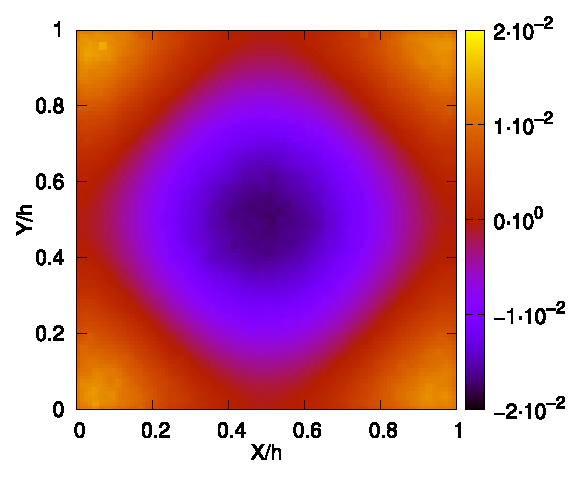
\includegraphics[width=0.49\textwidth]{gfx/fcm_gauss_3pt}}\label{fig:ibm_gauss3pt}
  \subcaptionbox{Peskin 3pt}{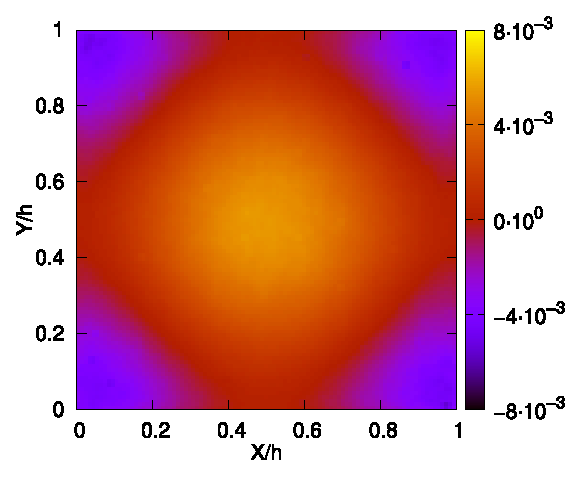
\includegraphics[width=0.49\textwidth]{gfx/fcm_peskin_3pt}}\label{fig:ibm_peskin3pt}
  \subcaptionbox{BM 3pt}{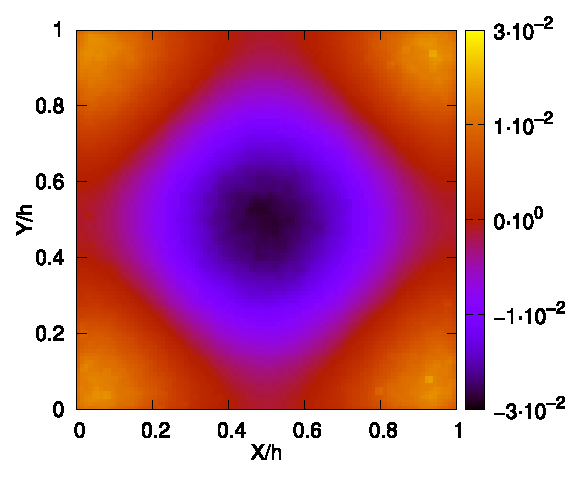
\includegraphics[width=0.49\textwidth]{gfx/fcm_bm_3pt}}\label{fig:ibm_bm3pt}
  \subcaptionbox{Gaussian 10pt}{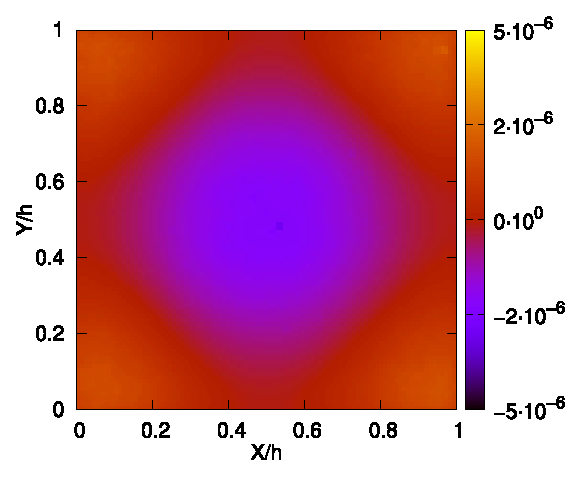
\includegraphics[width=0.49\textwidth]{gfx/fcm_gauss_10pt}}\label{fig:ibm_gauss10pt}
  \caption{Variance of the hydrodynamic radius inside a cell (2D slice at $z=L/2+h/2$ of a 3D system) for different kernels in \gls{FCM}. Test were carried out in a cubic box of size $L=32a$.}
\end{figure}
We test accuracy by measuring the translational invariance through the self mobility, $M_0$, of a particle being pulled. In particular, we measure the variance of the hydrodynamic radius (using $a = 6\pi\eta M_{0}$) inside a grid cell.
Error is computed as
\begin{equation}
  \label{hydroerr}
  E_a(\vec{r}) = \left|1 - \frac{a(\vec{r})M_{0}}{6\pi\eta}\right|
\end{equation}
Where the self mobility is computed using the well known periodic correction for the Stokes drag of a sphere\cite{Hasimoto1959}.

\begin{equation}
  M_{0}(a,L) = \frac{1}{6\pi\eta a}\left[1-b\frac{a}{L} + \frac{4\pi}{3}\left(\frac{a}{L}\right)^3 - c \left(\frac{a}{L}\right)^6\right]
\end{equation}
Where the factors $b$ and $c$ are
\begin{equation}
  \begin{aligned}
  b &:= 2.83729748\\
  c &:= \frac{16\pi^2}{45} + 23.85
  \end{aligned}
\end{equation}
\begin{figure}
\label{fig:ibm_hydrovar}
\includegraphics[width=\textwidth]{gfx/ibm_hydrodeviation}  
  \caption{Deviation from the average hydrodynamic radius inside a cell in the $x$ direction. Shown here is the error computed by evaluating eq. \eqref{hydroerr} inside a range $x=[0, 1]h$ with the mean substracted. Since the signal is symmetric only the range $[0.5, 1]h$ is presented.}
\end{figure}


\section{Inertial Coupling Method (ICM)}

\begin{itemize}
\item This is the algorithm described in \cite{Balboa2014}, but we neglect the excess mass of the particles.
\item Spatial discretization is done in an staggered grid, similar to FIB.
\item We recover the inertial terms in eq. \eqref{eq:navierstokes}. Using the projection method described in sec. \ref{sec:bdhi} we get
  \begin{equation}
    \dot{\vec{\fvel}} = \rho^{-1} \oper{P}\left(\vec{\mathfrak{f}} + \tilde{\vec{f}}\right)
  \end{equation}
  Where the new force, $\vec{\mathfrak{f}}$, includes the advective and diffusive terms
  \begin{equation}
    \vec{\mathfrak{f}} = -\rho\nabla\cdot (\vec{\fvel}\otimes\vec{\fvel}) + \eta\nabla^2\vec{\fvel}
  \end{equation}

\item We apply the projection operator in Fourier space, as we did in, for instance, sec. \ref{sec:fcm}. However, since we now have to solve the temporal variation of the velocity and we have non-linear terms, the diffusive and advective terms are be evaluated in real space. In ICM, the divergence of the noise is also evaluated in real space.
\item Temporal discretization: Second-order accuracy (since we assume there is no excess mass) mid point predictor-corrector scheme
  \begin{equation}
    \label{eq:icmalgo}
    \begin{aligned}
      &\vec{\ppos}^{n+\half} = \vec{\ppos}^n + \frac{\dt}{2}\oper{J}^n\vec{\fvel}^n\\
      &\rho\frac{\vec{\fvel}^{n+1} - \vec{\fvel}^n}{\dt} = \oper{P}\left(\vec{\mathfrak{f}}^{n+\half} + \tilde{\vec{f}}^{n+\half} \right)\\
      &\vec{\ppos}^{n+1} = \vec{\ppos}^n + \frac{\dt}{2}\oper{J}^{n+\half}\left(\vec{\fvel}^{n+1} + \vec{\fvel}^{n}\right)
  \end{aligned}
\end{equation}

\item Temporal discretization is similar to the mid point predictor-corrector schemes in FIB, but the convective term is discretized using a second order explicit Adams-Bashforth method (eq. 35 in \cite{Balboa2014}).
  \begin{equation}
    \nabla\cdot (\vec{\fvel}\otimes\vec{\fvel})^{n+\half} = \frac{3}{2} \nabla\cdot (\vec{\fvel}\otimes\vec{\fvel})^n - \half \nabla\cdot (\vec{\fvel}\otimes\vec{\fvel})^{n-1}
  \end{equation}
  Advection is therefore stored each step to be reused in the next.
  
  The diffusive term is discretized to second-order by
  \begin{equation}
    \nabla^2\vec{\fvel}^{n+\half} = \half\nabla^2\left(\vec{\fvel}^{n+1} + \vec{\fvel}^{n}\right)
  \end{equation}

  Replacing these equations into \eqref{eq:icmalgo} and solving for the velocity at $n+1$ leads to the full form of the velocity solve, depending only on the velocity from previous time steps

  \begin{equation}
    \label{eq:icmfluidvel}
    \begin{aligned}
      &\vec{\fvel}^{n+1} = \tilde{\oper{P}}\vec{g}^n =\tilde{\oper{P}}\Big[    \left(\frac{\rho}{\dt}\mathbb{I} + \frac{\eta}{2}\nabla^2\right)\vec{\fvel}^n- \\
      & \frac{3\dt}{2} \nabla\cdot (\vec{\fvel}\otimes\vec{\fvel})^n - \frac{\dt}{2} \nabla\cdot (\vec{\fvel}\otimes\vec{\fvel})^{n-1}+\\
    &\oper{S}\vec{F}^{n+\half} + \nabla\cdot\mathcal{Z}^n \Big]
  \end{aligned}
\end{equation}
Where the modified projection operator is defined as
\begin{equation}
  \tilde{\oper{P}} :=\left(\frac{\rho}{\dt}\mathbb{I} - \frac{\eta}{2}\nabla^2\right)^{-1}\oper{P} 
\end{equation}
And is applied in Fourier space.
\item The full algorithm can be summarized as follows:
  \begin{enumerate}
  \item Take particle positions to time $n+\half$: $\vec{\ppos}^{n+\half} = \vec{\ppos}^n + \frac{\dt}{2}\oper{J}^n\vec{\fvel}^n$ 
  \item Spread particles to the staggered grid: $\oper{S}\vec{F}^{n+\half}$
  \item Compute and store advection: $\nabla\cdot (\vec{\fvel}\otimes\vec{\fvel})^n$
  \item Compute the rest of the terms in $\vec{g}$ in eq. \eqref{eq:icmfluidvel}, using the just computed advective term in addition to the one stored in the previous step.
  \item Take $\vec{g}$ to Fourier space and apply $\tilde{\oper{P}}$: $\fou{\vec{\fvel}}^{n+1} = \fou{\tilde{\oper{P}}}\fou{\vec{g}}$
  \item Take $\fou{\vec{\fvel}}^{n+1}$ back to real space.
  \item Evaluate particle positions at $n+1$ by interpolating: $\vec{\ppos}^{n+1} = \vec{\ppos}^n + \frac{\dt}{2}\oper{J}^{n+\half}\left(\vec{\fvel}^{n+1} + \vec{\fvel}^{n}\right)$
  \end{enumerate}
Since we are describing a triply periodic algorithm, we can use the discrete form of the differential operators for a staggered grid devised in previous sections (see sec. \ref{sec:staggered} and \ref{sec:fib}). 
\item Some test of the algorithm, maybe the MSD of a particle? or a high Reynolds plot of the fluid velocity around a sphere
\end{itemize}

\chapter{Monte Carlo}
Monte Carlo schemes available in \uammd

\section{Hard spheres}
Just mention that it is present.

\section{Metropolis Adjusted Langevin Algorithm (MALA)}
Force biased, like Metropolis Monte Carlo but leveraging the forces. Amounts to performing a \gls{BD} simulation step and then use the positions, forces and energies of the old and new configurations to decide wether to accept it or not with a Metropolis-like probability.

We can interpret the Euler-Maruyama Brownian Dynamics scheme in eq. \eqref{eq:eulermaruyama} (with $M=1$) as a Markov chain with a transition kernel following a strictly positive probability transition density defined as\todo{De donde sale esto?}
\begin{equation}
  \label{eq:malakernel}
  p( \vec{Q}^n, \vec{Q}^{n+1}) = (4\pi \kT\dt)^{3/2}\exp\left(\frac{\left|\vec{Q}^{n+1} - \vec{Q}^n + \dt\vec{F}^n\right|^2}{4\kT\dt}\right)
\end{equation}
Where $\vec{Q}^n:={\vec{\ppos}_1^n, \vec{\ppos}^n_2, ..., \vec{\ppos}^n_N}$ represents the positions of all particles at time step $n$.
%This is refered to as the unadjusted Langevin algorithm\cite{Roberts1996}.
On the other hand, the Langevin equation \eqref{eq:bd} in equilibrium presents a probability density given by
\begin{equation}
  \label{eq:malatarget}
  \pi(\vec{Q}) = Z^{-1}\exp\left(-\frac{U(\vec{Q})}{kT}\right)
\end{equation}
Where the entropy is defined as $Z = \int\exp\left(-U(\vec{Q})/\kT\right)$ and $U(\vec{Q})$ is the internal energy (such that $\vec{F} = -\nabla U$).

Once we have a proposed transition kernel (eq. \eqref{eq:malakernel}) and and a target probability density (the equilirbium one in eq. \eqref{eq:malatarget}) we can use the Metropolis-Hastings method to design an updating scheme, refered to as MALA\cite{Roberts1996}\cite{Besag1994}.

Instead of sampling configurations using the Euler-Maruyama scheme (as discussed in sec. \ref{sec:bd}) we now propose a new configuration using eq. \eqref{eq:eulermaruyama} as
\begin{equation}
  \widetilde{\vec{Q}}^{n+1} = \vec{Q}^n + \dt\vec{F}^n + \sqrt{2\kT\dt}\vec{\widetilde{\mathcal{W}}}^n
\end{equation}

And accept it with a Metropolis probability given by

\begin{equation}
  \alpha(\vec{Q}^n, \widetilde{\vec{Q}}^{n+1}) = \text{min}\left(\frac{p(\widetilde{\vec{Q}}^{n+1},\vec{Q}^{n})\pi(\widetilde{\vec{Q}}^{n+1})}{p(\vec{Q}^{n}, \widetilde{\vec{Q}}^{n+1})\pi(\vec{Q}^{n})}\right)
\end{equation}

Numerically, this can be done by drawing an uniform random number $\xi^n \in [0,1]$ and accepting the new configuration only if $\xi^n<\alpha(\vec{Q}^n, \widetilde{\vec{Q}}^{n+1})$.

In contrast with the naive Metropolis-Hasting algorithm, that blindly proposes configurations, MALA proposes configurations that always have a higher propability in $\pi$, increasing the chances of acceptance.

\begin{itemize}
\item We are not restricted to using the same value for $\dt$ in all steps, since in an MCMC algorithm it has lost its meaning as a \emph{time step} and it is now simply a parameter describing the \emph{distance} in phase space between two given configurations. As such we can tune it to get a desired configuration acceptance ratio.
\item Although it is useful to thermalize or initialize configurations, testing suggests that hard steric repulsion between particles (like LJ) requires such a small time step to ensure a given acceptance ratio that the algorithm becomes unusable. In these cases plain BD is preferable.
\item For tuning the jump step, we measure the acceptance ratio every once in a while, if it is lower than the target the jump step is decreased (and increased if it is larger). We increase the jump step slowly (a 2\% increase) and decrease it fast (a 10\%). this decision stems from optimization.
\item Another disadvantage of MALA is that, for instance, in a thermalized, equilibrium configuration the energy change coming from moving all particles in the system grows, in average, with the number of particles. This results in the optimal jump step decreasing with the number of particles.
  \begin{figure}[H]
    \label{fig:malastep}
    \centering    
    \subcaptionbox{Soft potential}{\includegraphics[width=\textwidth]{gfx/malasoft}}\label{fig:malastepsoft}
    \subcaptionbox{LJ potential}{\includegraphics[width=\textwidth]{gfx/malalj}}\label{fig:malasteplj}
    \caption{Optimal time step in MALA for several configurations.}
  \end{figure}
  
\end{itemize}
\subsection*{Use in UAMMD}

\begin{itemize}
\item Use like any other Integrator, will query its Interactors for both force and energy.
\item The step size will be autotuned until it reaches the target one.
\end{itemize}
\begin{code2}[Example of the creation of a MALA \emph{Integrator} module.]{label=code:mala}
#include<uammd.cuh>
#include<Integrator/MonteCarlo/ForceBiased.cuh>
using namespace uammd;
//A function that creates and returns a MALA integrator
auto createIntegratorMALA(UAMMD sim){   
  MC::ForceBiased::Parameters par;
  //Inverse of temperature
  par.beta = 1.0/sim.par.temperature;	
  //Initial step length.
  //It will be optimized according to the target acceptance ratio
  par.stepSize = sim.par.dt;
  //Desired acceptance ratio 
  par.acceptanceRatio = sim.par.accRatio;
  auto mala = std::make_shared<MC::ForceBiased>(sim.pd, par);
  return mala;
}
\end{code2}



\begin{itemize}
\item Finishing words about methodology
\item A word about all things implemented in UAMMD thus far
\item Putting it all together
\item An outline of all the phisics that can be done with the algorithms and implementations thus far
\item Future direction and additions to the algorithms in this part
\item Introduce next part, novel algorithms and physics.

\end{itemize}
\cleardoublepage
\part{Novel algorithms and physics for complex fluids}\label{pt:algo}

In this part of the manuscript we will go through several novel, \gpu-focused, algorithms that have been developed during this thesis.
In particular, we will discuss four new algorithms; two of them solving the Stokes equation (see eq. \eqref{eq:stokes}) for hydrodynamics and the other two solving the, not yet introduced, Poisson equation (see eq. \eqref{eq:ttpoisson}) for electrostatics.
In chapter \ref{sec:q2D} we introduce a novel algorithm for solving the Stokes equation in quasi 2D geometries, in which particles are restricted to move in a periodic plane while embedded in a fluid that is either open (quasi 2D) or non existent (true 2D) in the third direction.
Later, in chapter \ref{sec:dpstokes} we solve the Stokes equation again but this time letting the particles move freely inside a doubly periodic domain (periodic in the plane and open in the third direction), introducing the possibility of placing walls at the domain limits, creating slit or walled geometries.
The doubly periodic Stokes algorithm will be the last methodology for hydrodynamics in this manuscript. We will use the two next chapters in this part to introduce two algorithms for electrostatics (by solving the Poisson equation)\footnote{The algorithms for electrostatics make use of the toolset developed for \gls{FCM} and \gls{PSE} in previous chapters, which is the reason why its introduction was delayed up to this point}. We will start by describing a method for computing the electrostatic interactions of a group of charged particles in a triply  periodic environment in chapter \ref{ch:tppoisson}. Finally, in a similar way as done with Stokes, we will compute electrostatic interactions in a doubly periodic environment (with the possibility of placing surface charged walls at the domain limits).
\begin{itemize}
\item New contributions are related to complex fluids in confined geometries
\item Hydrodynamics in slit channels are key in several contexts of technological and biological significance.
\item Introduce star polymers
\end{itemize}

\chapter{Hydrodynamics under quasi two dimensional confinement}\label{sec:q2D}
\begin{figure}[h]
  \centering
  \includesvg[width=\columnwidth]{gfx/q2d}
  \caption{Representation of a colloidal system under soft confinement in the perpendicular ($z$) direction. Particles are confined via some external potential that distributes them near $z=0$ with a typical width $\delta$. The confining forces acting on the particles are propagated to the plane via the Oseen tensor (orange lines).}
  \label{fig:q2dsch}
\end{figure}

In this section we will develop algorithms to study the dynamics of a group of colloidal particles whose movement is constraint in the $z$ direction by some external force (see fig. \ref{fig:q2dsch}) while submerged in an otherwise unbounded three dimensional fluid. We refer to this geometry as quasi 2D (q2D for short). As opposed to a situation in which both the particles \emph{and} the fluid are restricted to the plane (true 2D or t2D) or when both are unbounded in the three directions (true 3D or t3D). In the limit when the confining force is infinetly stiff, particles move in an strictly two dimensional plane. This can be used to model, for instance, the transport the properties of systems at a fluid-fluid or air-fluid interfaces. 

Besides being common in subcellular biology, there are several examples of this constrained dynamics systems in a wide variety of industrial applications, like food, creams, or crude oil (e.g., asphaltenes near water interfaces).
On the other hand, the transverse diffusion of proteins embedded in lipid bilayers controls their biological function\cite{MembraneDiffusion_Review}.
Note that although confined to the membrane plane, these proteins will be subject to relatively large spatial fluctuations.

In general, diffusion of colloidal particles confined to two-dimensional surfaces is a key transport mechanism in several contexts of technological and biological significance.

As to the physical phenomena that actually constraints the particles to a plane we have, for instance the so-called Pickering emulsions, which are stabilized by the spontaneous absorption of colloidal particles to the fluid-fluid interface.

Colloids might also be trapped in fluid-fluid interfaces and interact via capillary[2] or electrostatic[3] forces. By placing walls, particles can be forced to diffuse in a plane\cite{Diffusion2D_Experiments_Rice}. 

A standing pressure wave with hundreds of megahertz or more creates an ultrasound potential which moves heavy colloidal particles towards two-dimensional traps formed at the node of the pressure wave (or the valleys if particles are lighter than the fluid)[6,7]. The resulting ultrasound potential is harmonic, leading to a Gaussian colloidal dispersion around the pressure node[7].

Similar harmonic traps can be obtained by laser tweezers[8]. Other forms of (non-Gaussian) traps can be prepared using electric fields (maybe leading to barometric-like density profiles).

In future sections, we will study the diffusive phenomena arising in this special geometry. For now, lets lay the algorithmic machinery necessary to simulate it.

Lets start by considering a suspension of colloidal particles confined near $z=0$ by a strong confining potential submerged in an otherwise unbounded three dimensional incompressible fluid. As we saw in chapter \ref{ch:bdhi}, forces acting on the particles are propagated to the whole fluid, due to the its incompressibility, via the Oseen tensor. This results in part of the momemtum introduced in the fluid by the confining force acting on one particle (which acts in the normal direction) being propagated over the plane. As we will soon see, the resulting hydrodynamic drag acts like a flow source which tends to expel other particles around it. This can be interpreted as the flow in the plane having a positive divergence, which makes the fluid (as seen from the plane) being effectively compressible. We will see that this effect naturally arises in a particle based description (\gls{BDHI}) through an effective plane mobility with non zero divergence\cite{Pelaez2017}.

There are several ways to gradually transform a perfect 2D confinement into an isotropic 3D distribution and, as illustrated in fig. \ref{fig:q2dsch}, we model the case where the 2D interface of colloids becomes Gaussianly blurred. In particular, we consider a suspension of colloids confined in the $z$ direction around some height, $z=0$, by an harmonic potential of the form
\begin{equation}
U(z)=\half K_sz^2
\end{equation}
applied to each individual particle.
The spring constant $K_s$ controls the width, $\delta$, of the Gaussian distribution of particles in the $z$ direction.
\begin{equation}
  \delta = \left(\frac{\kT}{K_s}\right)^{1/2}
\end{equation}
We can use this as a slider to go from t3D, in the limit $K_s\rightarrow 0$, to q2D when $K_s\rightarrow\infty$.
The dynamics of the system are then governed by eq. \eqref{eq:bdhi} with an Oseen-like mobility (like the \gls{RPY} one). Note that solvent inertial effects can also be incorporated by using the \gls{ICM} in sec. \ref{sec:icm}.

Thus far, all the algorithms we have developed for solving \eqref{eq:bdhi} (or more generally eq. \eqref{eq:navierstokes}) deal with either fully open or triply periodic boundary conditions. However, now the perpendicular direction should be open while leaving the plane periodic.

To be fair, our mathematical infrastructure allows to discretize the Stokes operator in any geometry to accommodate any boundary conditions. But since our implementations rely on the \gls{FFT} to be efficient and \gpu-friendly these modifications are not straight forward. 

One approach to deal with this is to simply use the triply periodic algorithms with a box with width ,$L_z\gg \delta$, large enough to neglect finite-size effects. However, since hydrodynamics are long ranged in nature we will be forced to perform a full finite-size analysis to ensure the convergence of the measured properties.

In future sections, we will describe a family of pseudo-spectral algorithms capable of dealing with non periodic boundary conditions. For the moment, lets adapt the already developed \gls{FCM} to the limit of strict confinement (q2D). Lets see how we can compute the Fourier expression of a Green's function specific for q2D.

\section{The Force Coupling Method in quasi 2D}

We want to take the mathematical limit of eq. \eqref{eq:bdhi} when $K_s\rightarrow\infty$ and hence particles move strictly in the plane $z=0$. Although it is possible to take this limit formally the general theory for it is quite complex. Luckily we can elaborate some simple arguments an assumptions to make this in a trivial way.

We start with the realization that, given that the particles are restricted to a plane, the mobility tensor can be reordered in a diagonal blocked arregement 

\begin{equation}
\tens M=\left[\begin{array}{cc}
\tens M^{\parallel} & \tens M^{\parallel,\perp}\\
\left(\tens M^{\parallel,\perp}\right)^{T} & \tens M^{\perp}
\end{array}\right]=\left[\begin{array}{cc}
\tens M^{\parallel}\\
 & \tens M^{\perp}
\end{array}\right]
\end{equation}
Where the parallel mobility (in the $x,y$ plane) is decoupled from the perpendicular one (in $z$). We can see this by understanding that a perpendicular force cannot induce motion on the plane, since that would break symmetry. Equivalently, a parallel force cannot take a particle out of plane. On the other hand, the confinement does not cause a free energy gradient in the plane (since it is uniform in it).

This means that we can simply remove the $z$ component in our description and write
\begin{equation}
  d\vec{\ppos} = \tens{M}^{\parallel}\vec{F}dt + \sqrt{2\kT \tens{M}^{\parallel}}d\vec{\widetilde{W}^{\parallel}} + \kT\left(\partial_{\vec{\ppos}}\cdot\tens{M}^{\parallel}\right)\dt
\end{equation}
Where the particle positions and forces, the mobility and the noise are now defined only in the plane.
As we will soon see, in this case the thermal drift cannot be ommited.

Up until now, we have not included the action of the thermal drift in the \gls{FCM}. We can use the general definition of the mobility tensor in eq. \eqref{eq:bdhimob} as the double convolution of the Green's function with the kernel to write the thermal drift in the a similar form

\begin{equation}
  \label{eq:q2Ddriftconv}
  \begin{aligned}
    \partial_{\vec{\ppos}}\tens{M}_{ij}=& \int\delta_a(\vec{\ppos_i} -\vec{r})\nabla\cdot\tens{G}(\vec{r},\vec{r}')\delta_a(\vec{\ppos_j} -\vec{r})d\vec{r}d\vec{r}' =\\
     &\int\delta_a(\vec{\ppos_i} -\vec{r})\tens{G}(\vec{r},\vec{r}')\nabla\delta_a(\vec{\ppos_j} -\vec{r})d\vec{r}d\vec{r}'    
\end{aligned}
\end{equation}

Where the second equality can be easily proven via integration by parts. A formal proof of this description can be found in\cite{Donev2014}. One simple way to see this is by computing the contribution of the thermal drift to the fluid velocity in Fourier space. Since we have periodic boundary conditions (remember that our description is now in the plane) the divergence commutes in Fourier space we can simply write
\begin{equation}
  i\vec{k}\cdot\fou{\tens{G}}\mathfrak{F}\left[\delta_a(\vec{\ppos}_j -\vec{r})\right] = \fou{\tens{G}}\cdot \left(i\vec{k}\mathfrak{F}\left[\delta_a(\vec{\ppos}_j -\vec{r})\right]\right)
\end{equation}
Which evidences that we can take the divergence in eq. \eqref{eq:q2Ddriftconv} from the Green's function to the kernel.
Once we have this, we can include the thermal drift in the \gls{FCM} framework as an external fluid forcing by redefining the force term in eq. \eqref{eq:fcmvel} as

\begin{equation}
  \label{eq:q2Ddrifasforce}
  \vec{f} = \oper{S}\vec{F} + \vec{\partial}\oper{S}(\kT)
\end{equation}

Where $\partial_\alpha\oper{S} = \partial\oper{S}/\partial r_\alpha$ is the derivative of the kernel, in this case a Gaussian. Note that we can either spread the quantity $\kT$ to the grid using the derivative of the kernel, or use the regular kernel and \emph{ik} differentiate the term in Fourier. However, since the second option would require to isolate the Fourier transform of the thermal drift it is in principle not worth it over the simple evaluation of the derivative of a Gaussian in real space.
\footnote{In fact, in the case of a Gaussian, we can spread a single quantity by using $\partial\phi_G(r) = 2\sigma_ar\phi_G(r)$ and spreading $\vec{F} + 2\kT\sigma_a\vec{r}$.}

Interestily enough, interpreting the thermal drift as an external force gives us some insight into the physical effects of the non zero divergence of the mobility. In particular, because the quasi 2D mobility will still be translationally invariant and isotropic in the plane, we can still assume the general form in eq. \eqref{eq:bdhimobgeneral}. In general, at long distances we have the Oseen approximation for $f(r)$ and $g(r)$\footnote{Interpreting that $M_0=1$ for the mobility written in this way.}
\begin{equation}
  f(r) \approx g(r) \approx \frac{1}{8\pi\eta} \text{ for } r\gg a
\end{equation}
Which yields a zero divergence in true 3D and true 2D. However, in quasi 2D we have
\begin{equation}
  \nabla\cdot\tens{M}_{\text{q2D}} \approx \frac{1}{8\pi\eta r}\frac{\vec{r}}{r^3} \text{ for } r\gg a
\end{equation}
Using eq. \eqref{eq:q2Ddrifasforce} we can see that this is equivalent to having the particles interact via a repulsive electrostatic potential
\begin{equation}
  U_{\text{eff}}(r) = \frac{3a}{4r}\kT
\end{equation}
It is important to keep in mind, though, that this force is stochastic in nature and is in fluctuation-dissipation balance with the thermal fluctuations. The physical origin of this effective force comes from the rapid momentum transport perpendicular to the plane, which makes the plane in the flow behave with an effective non zero compressibility. This makes the quasi 2D system inherently different from a distribution of charges. In fact, since hydrodynamics will not change the equilibrium properties, these equations still describe, in the absence of other particle interactions, an ideal gas without structure. Nevertheless, this interpretation allows us to see the dramatic (purely hydrodynamic) effect of the confining force in the plane flow and highlights the necessity of including the thermal drift into the quasi 2D description.

We can now compute the Green's function in quasi 2D by convolving the 3D Oseen tensor in eq. \eqref{eq:bdhioseen} with a Gaussian and integrating it analytically along the $z$ direction

\begin{equation}
  \label{eq:q2dGreenintegral}
  \begin{aligned}
  \fou{\tens{G}}_{\text{q2D}}(\vec{k} = (k_x, k_y)) &= \frac{1}{2\pi\eta}\int_{k_z} \frac{dk_z}{(k')^2}\exp\left(-\frac{a^2k_z^2}{\pi}\right)\left( \mathbb{I} - \frac{\vec{k}'\otimes\vec{k}'}{(k')^2}\right) \\
  &= \eta^{-1}\left(g_k(k)\vec{k}_{\perp}\otimes\vec{k}_{\perp} + f_k(k)\vec{k}\otimes\vec{k}\right)
\end{aligned}
\end{equation}
Where $\vec{k}' = (k_x, k_y, k_z)$ is the three dimensional wavenumber and we recall that unless stated otherwise, in quasi 2D vectors are defined in $\mathbb{R}^2$. Additionally $\vec{k}_\perp := \vec{k}\times\hat{z} = (k_y, -k_x)$ is a vector perpendicular to $\vec{k}$. Note that we also had to convolve with the Gaussian kernel in the $z$ direction, since it is not included in our purely 2D description. The convolution with the $(x,y)$ kernel is performed explicitly via spreading in \gls{FCM}.
Note that this has restricted our algorithm to a Gaussian kernel, with its advantages and disadvantages. However, a different kernel can be used if it has an analytical Fourier form that allows the integral in eq. \eqref{eq:q2dGreenintegral} to be solved analytically\footnote{The anaylical form of eq. \eqref{eq:q2dGreenintegral} is not actually needed if somehow $f_k$ and $g_k$ are tabulated.}.

Solving eq. \eqref{eq:q2dGreenintegral} yields
\begin{equation}
  \label{eq:q2dfg}
  \begin{aligned}
    g_{k}\left(k\right) & = \frac{1}{2}\left[1-{\erf}\left(\frac{ka}{\sqrt{\pi}}\right)\right]\exp\left(\frac{k^2a^2}{\pi}\right)\\
    f_{k}\left(k\right) & = \left(\frac{1}{2} - \frac{k^{2}a^2}{\pi}\right)g_k(k) - \frac{ka}{2\pi}
  \end{aligned}  
\end{equation}

We can also write the Green's function for true 2D by redefining $f_k$ and $g_k$ (by simply not integrating in $z$ nor convolving with the kernel in $z$)
\begin{equation}
  \label{eq:t2dfg}
  \begin{aligned}
    g_{k}\left(k\right) & = 0\\
    f_{k}\left(k\right) & = \frac{1}{k}
  \end{aligned}  
\end{equation}
\todo{Rafa, aqui puedo añadir G para saffman, tienes alguna referencia por ahi?, quizas esto deberia ir mas en ``future directions''}

This concludes all the modifications to the \gls{FCM} (as described in sec. \ref{sec:fcm}) required to simulate a quasi 2D system. Note that by using eq. \eqref{eq:t2dfg} instead of eq. \eqref{eq:q2dfg} our algorithm is also capable of simulating a true 2D system. In fact, any 2D hydrodynamic kernel can be used as long as $f_k$ and $g_k$ are known\footnote{Note that the analytical expression is not actually needed and it could be, for instance, computed numerically and then tabulated}. For instance, the Saffman mobility could be used to model the diffusion of proteins in a lipid membrane\cite{Saffman}.

Finally, for convenience, we can use a similar trick as we did for \gls{PSE} in eq. \eqref{eq:psenoise} to separate the contributions of the noise in eq. \eqref{eq:fcmvel} as

\begin{equation}
  \begin{aligned}
    \fou{\tens{Z}}_k := \sqrt{\frac{2\kT}{\eta k^3}}\left(\sqrt{f_k(k)}\vec{k}_\perp\fou{\tens{Z}}^1_k + \sqrt{g_k(k)}\vec{k}\fou{\tens{Z}}^2_k\right)
  \end{aligned}
\end{equation}
Where $\fou{\tens{Z}}^{1,2}_k$ are independent Wienner processes. The same concerns about the delicate conjugacy properties of the noise we discussed in sec. \ref{sec:fcm} are applicable here.
% This integral can be done analitically to give
%\begin{equation}
%  \fou{\tens{M}}_{\text{q2D}} = \frac{1}{\eta k^3}\left( \half\vec{k}_{\perp}\otimes\vec{k}_{\perp} + \frac{1}{4}\vec{k}\otimes\vec{k}\right)
%\end{equation}


\subsubsection*{Use in UAMMD}
\begin{itemize}
\item This is used as the rest of the \emph{Integrators}
\item A templated base class BDHI::BDHI2D can be specialized for any 2D greens function by providing $f_k$ and $g_k$, see the online documentation for more information. The aliases BDHI::True2D and BDHI::Quasi2D are provided for the hydrodynamic kernels described in the previous section.
\item Tolerance controls the support of the Gaussian kernels and the size of the grid similarly as in \gls{FCM}.\todo{This is not actually implemented, it is just hardcoded to 1e-4}
\end{itemize}
\todo{I could implement the same thing for FCM, generalizing the module for any $f_k$ and $g_k$ as long as they do not have thermal drift, which is not implemented in 3D. Maybe this could be done for FIB, where thermal drift is obtained via RFD.}
\begin{code2}[Example of the creation of a quasi 2D \emph{Integrator}.]{label=code:q2D}
#include<uammd.cuh>
#include<Integrator/Hydro/BDHI_quasi2D.cuh>
using namespace uammd;
//A function that creates and returns a quasi 2D integrator
auto createIntegratorQ2D(UAMMD sim){
  //Choose the hydrodynamic kernel
  using Hydro2D = BDHI::Quasi2D;
  //using Hydro2D = BDHI::True2D;
  Hydro2D::Parameters par;
  par.temperature = sim.par.temperature;
  par.viscosity = sim.par.viscosity;
  par.hydrodynamicRadius = sim.par.hydrodynamicRadius;
  par.dt = sim.par.dt;
  par.tolerance = sim.par.tolerance;
  par.box = sim.par.box;
  auto q2d = std::make_shared<Hydro2D>(sim.pd, par);
  return q2d;
}
\end{code2}

\newpage

\chapter{Hydrodynamics in doubly periodic geometries}\label{sec:dpstokes}
We develop an algorithm to solve the incompressible Stokes equation \eqref{eq:stokes} without fluctuations in a \gls{DP} domain of size $L_{x,y}$ (we will assume $L_x=L_y$, which can then be easily generalized). Thus, we want to solve
\begin{equation}
  \label{eq:dpstokes}
  \begin{aligned}
    &\nabla p_{\dpr} - \eta\nabla^2\vec{\fvel}_{\dpr} = \vec{f}\\
    &\nabla\cdot\vec{\fvel}_{\dpr} = 0
\end{aligned}
\end{equation}
With $z\in(-\infty, \infty)$ and free-space \glspl{BC} in $z$, assuming that $\vec{\fvel}_{\dpr}$ is bounded as $|z|\rightarrow\infty$. The plane $(x,y)$ is periodic as in quasi 2D.

Here $p$ is the pressure and the fluid forcing includes the particle forces and torques (similarly as with \gls{FCM} in sec. \ref{sec:fcm})
\begin{equation}
  \vec{f}(\vec{\fpos}) = \oper{S}\vec{F} + \half\nabla\times\oper{S}_{\tau}\vec{\tau}
\end{equation}

We assume that the fluid forcing is zero outside a domain $z\in [-H, H]$. In the case of an unbounded fluid this domain is arbitrary and physically meaningless, serving only to define a numerical domain for our grid-based solver. The same thing happens in the case of a bottom wall with the top limit at $z=H$. Furthermore, assuming $\vec{f}(|z|>H) = 0$ allows us to define a set of \glspl{BC} more easily.

Our solver is periodic in the plane $(x,y)$ (as in quasi 2D). In the $z$ direction, by incorporating different \glspl{BC}, we distinguish between three modes:
\begin{enumerate}
\item Unbounded in $z$, $z\in(-\infty, \infty)$. $\vec{\fvel}_{\dpr}$ is bounded as $|z|\rightarrow\infty$.
\item A no-slip  wall at the bottom of the domain, $z=-H$ (unbounded at $z>H$). $z\in [-H, \infty)$.
  The no-slip \gls{BC} for the wall is simply
  \begin{equation}
    \label{eq:dpstokesbwvelbc}
    \vec{\fvel}_{\dpr}(z=-H) = 0.   
  \end{equation} 
\item A slit channel, with no-slip walls located at $z=-H$ and $z=H$. $z\in [-H, H]$. Besides the \gls{BC} for the bottom wall, we add a similar one for the top one
  \begin{equation}
    \label{eq:dpstokestwvelbc}
    \vec{\fvel}_{\dpr}(z=H) = 0.
  \end{equation}
\end{enumerate}
The unbounded mode allows to simulate systems were particles are not restricted to a plane, so $\delta>0$. Additionally the other modes can be used in a variety of simulations. For instance, the bottom wall mode can be used to model the hydrodynamics of a Quarts Crystal Microbalance (QCM)\todo{More about it?}.

In the free-space case we can simply define the limits of the domain far enough from the particles so that $\vec{f}(z\notin [-H,H]) = 0$. However, in the presence of a wall we must ensure that the force goes smoothly to zero at the wall. We enforce this by substracting the envelope of a given particle centered at its image about the wall. We can thus redefine the kernel close to the wall\footnote{Closer than the kernel's support, which effectively means everywhere.} as
\begin{equation}
  \label{eq:dpstokeskernel}
  \widetilde{\delta_a}(\vec{\fpos}-\vec{\ppos}_i) = \delta_a(\vec{\fpos}-\vec{\ppos}_i) - \delta_a(\vec{\fpos}-\vec{\ppos}^{\text{img}}_i)
\end{equation}
Were $\vec{\ppos}_i^{\text{img}}$ is the particle's point of reflection about the wall, defined as
\begin{equation}
  \label{eq:dpstokesimg}
  \begin{aligned}
  &\vec{\ppos}_i^{\text{img}_b} = \vec{\ppos}_i - 2(H+r_z)\hat{\vec{e}}_z, \quad \text{For the bottom wall}\\
  &\vec{\ppos}_i^{\text{img}_t} = \vec{\ppos}_i + 2(H-r_z)\hat{\vec{e}}_z, \quad \text{For the top wall}
\end{aligned}
\end{equation}
Being $\hat{\vec{e}}_z$ a unitary vector in the $z$ direction. The no-slip condition is then imposed by the fact that a particle at the height of a wall does not affect (nor it is affected by) the fluid. A visual representation of the effect of the images is available in fig. \ref{fig:dpstokesspread}.
\begin{figure}[h]
  \centering
  \includesvg[width=\columnwidth]{gfx/dpstokesspread}
  \caption{Representation of the image spreading in the \gls{DP} Stokes algorithm. Forces acting on particles (blue circles) are translated to the fluid as a force density. Due to images, part of the particle's force is zero near walls. Zero fluid forcing is depicted as white. A particle located at exactly the height of a wall has no effect on the fluid.}
  \label{fig:dpstokesspread}
\end{figure}

The \gls{DP} solver is vastly different from the \gls{FCM} family of methods we have seen thus far. The main similarity is that we also make use of the \gls{IBM}'s spreading and interpolation to communicate the particles and a grid.

Our approach consists of solving the Stokes equation in an ubounded domain, adding the effects of the walls afterwards as a correction. Thus we first solve eq. \eqref{eq:dpstokes} with free-space \glspl{BC} and $z\in (-\infty, \infty)$. Then we compute the final result in the presence of one or two walls as
\begin{equation}
  \label{eq:dpstokescorrsum}
  \begin{aligned}
  &\vec{\fvel} =   \vec{\fvel}_{\dpr} +   \vec{\fvel}_{\corr}\\
  &\vec{p} =   \vec{p}_{\dpr} +   \vec{p}_{\corr}
\end{aligned}
\end{equation}

For the corrections, we solve, analytically, eq. \eqref{eq:dpstokes} in the absence of forces with one or two slip walls. In particular we have
\begin{equation}
  \label{eq:dpstokescorr}
\begin{aligned}
    &\nabla p_{\corr} - \eta\nabla^2\vec{\fvel}_{\corr} = 0\\
    &\nabla\cdot\vec{\fvel}_{\corr} = 0  
\end{aligned}
\end{equation}
Solved in a domain with $z\in [-H,\infty)$ in the case of a bottom wall and $z\in [-H, H]$ in the case of a slit channel. Finally, we set slip \glspl{BC} at the walls so

\begin{equation}
  \label{eq:dpstokescorrbcs}
  \begin{aligned}
    &\vec{\fvel}_{\corr}(z=-H) = -\vec{\fvel}_{\dpr}(z=-H)\\
    &\vec{\fvel}_{\corr}(z=H) = -\vec{\fvel}_{\dpr}(z=H)    
\end{aligned}
\end{equation}
Where the second condition, at $z=H$, is imposed only in the case of a slit channel geometry.

In Appendix \ref{sec:bvp} we describe a fast and \gpu-friendly \gls{BVP} solver that solves one-dimensional \glspl{PDE} in the Chebyshev basis. Our strategy in the next sections will be to write equations for the velocity and pressure in a way that is compatible with this solver.

We will first discuss the free-space solver ($\vec{\fvel}_{\corr} = 0$ and $p_\corr=0$) and then see how to solve the correction in each case. 
\section{Free-space solver}
Let us start by writing the equations for the pressure (eq. \eqref{eq:stokespressure}) in Fourier space only in the plane $(x,y)$, which makes it easier to incorporate arbitrary \glspl{BC} in the $z$ direction.

\subsection*{Pressure solve}
By taking the divergence of eq. \eqref{eq:dpstokes} we eliminate the velocity
\begin{equation}
  \label{eq:dpstokespressure}
  \nabla^2 p = \nabla\cdot\vec{f}
\end{equation}
Transforming to Fourier space in the plane we get a one dimensional problem for each wave number
\begin{equation}
  \label{eq:dpstokesfreepressure}
  (\partial_{zz}-k^2)\fou{p} =
  % \begin{bmatrix}
  \left[
    i\vec{k},
    \partial_z\right]
  % \end{bmatrix}
  \cdot\vec{f}
\end{equation}
Where the wave vector $\vec{k}:=(k_x, k_y)$ is defined on the plane and has modulus $k^2 = k_x^2 + k_y^2$. The forces, $\vec{f}=(f^x, f^y, f^z)$ can be non-zero only inside a certain domain with $z\in [-H,H]$. Note that the pressure (and the forces) are Fourier transformed only in the plane, so that $\fou{p} :=\fou{p}(\vec{k}, z)$. As a matter of fact, the \gls{FCT} is employed here (see Appendix \ref{sec:fct}) to transform the signals in the $z$ direction to the Chebyshev basis, as this allows to use the \gls{BVP} solver and facilitates the evaluation of the derivatives in this direction (by using the relations for the Chebyshev coefficients introduced in Appendix \ref{sec:bvp}). Therefore we will work with the Chebyshev coefficients, $\fou{p}_n$ (or $\fou{\vec{f}}_n$), of the different quantities. We can solve the pressure outside the domain using that
\begin{equation}
    (\partial_{zz}-k^2)\fou{p} = 0, \quad \text{ for } z \notin [-H,H].
\end{equation}
Whose solution is
\begin{equation}
  \fou{p}(k, z) = C_1\exp(-kz) + C_2\exp(kz)
\end{equation}
By using the boundness of the pressure at $|z|\rightarrow\infty$ we can write the solution outside the domain
\begin{equation}
  \begin{aligned}
    &\fou{p}(k,z\le -H) = C_2\exp(kz)\\
    &\fou{p}(k,z\ge H) = C_1\exp(-kz)    
  \end{aligned}
\end{equation}
This implies
\begin{equation}
  \label{eq:dpstokespressurebcs}
  (\partial_z\pm k)\fou{p}(k, z=\pm H) = 0
\end{equation}
For a given wave number, $k$, the system in eq. \eqref{eq:dpstokesfreepressure} along the \glspl{BC} in eq. \eqref{eq:dpstokespressurebcs} constitute a \gls{BVP} that can be solved in Chebyshev space with the solver described in Appendix \ref{sec:bvp}.

Since this solver requires to define $z$ in the Chebyshev basis, we can apply $\partial_z$ in linear time by using recurrent relations on the Chebyshev coefficients (in this case of $\fou{f}^z$) instead of via \emph{ik} differentiation. As discussed in Appendix \ref{sec:bvp} and \ref{sec:fct}, the Fourier-Chebyshev\footnote{Fourier in the plane $(x,y)$ and Chebyshev in $z$.} coefficients $\fou{p}(\vec{k}, z)$ are computed via a hybrid \gls{FFT}-\gls{FCT}. Which amounts to performing the 3D \gls{FFT} of $\vec{f}$ periodic extended in $z$.

\subsection*{Velocity solve}
Once the Chebyshev coefficients for the pressure for each wave number are known we can write the equations for the three components of the velocity in Fourier space as

\begin{equation}
  \label{eq:dpstokesvel}
  \eta\left(\partial_{zz} -k^2\right)\fou{\vec{\fvel}} = 
  \begin{bmatrix}
    i\vec{k}\\
    \partial_z
  \end{bmatrix}
  \fou{p} -\fou{\vec{f}}
\end{equation}

Where the derivative of the pressure, $\partial_z\fou{p}$, can be computed via the Chebyshev coefficients of the pressure.

For the \glspl{BC} we know that outside the domain, where $\fou{\vec{f}} = 0$, the velocity satisfies
\begin{equation}
  \label{eq:dpstokesvelout}
  \eta\left(\partial_{zz} -k^2\right)\fou{\vec{\fvel}} = 
  \begin{bmatrix}
    i\vec{k}\\
    \partial_z
  \end{bmatrix}
  \fou{p}, \quad \text{ for } z \notin [-H,H]
\end{equation}
The \glspl{BC} for eq. \eqref{eq:dpstokesvelout} must be computed independently for the plane, $\vec{\fvel}^\parallel$, and perpendicular, $\vec{\fvel}^\perp$, velocities.
\subsubsection*{Parallel velocity solve}
Using the boundness of the velocity at $\pm\infty$, the solution of eq. \eqref{eq:dpstokesvelout} in the plane for $z \le -H \text{ and } z\ge H]$ is, respectively
\begin{equation}
  \label{eq:dpstokesparvel}
  \fou{\vec{\fvel}}^{\parallel} = \mp\frac{C_1\vec{k}\exp(\pm kz)\left(2zk\mp 1\right)}{4\eta ik^2} + C_2\exp(\pm zk).
\end{equation}
The derivative of eq. \eqref{eq:dpstokesparvel} can be written as
\begin{equation}
  \label{eq:dpstokesparvelder}
  \partial_z\fou{\vec{\fvel}}^{\parallel} = \pm k\fou{\vec{\fvel}}^{\parallel} + \frac{C_1i\vec{k}\exp(\pm kz)}{2\eta k}.
\end{equation}
We can make use of the previously computed solution for the pressure outside the domain,
\begin{equation}
  \label{eq:dpstokespresout}
\fou{p}(\vec{k}, z \le -H \text{ or } z\ge H]) = C_1\exp\left(\pm zk\right),
\end{equation}
to finally write the \glspl{BC} for the parallel velocity as
\begin{equation}
  \label{eq:dpstokesparvelbc}
  \left(\partial_z\pm k\right)\fou{\vec{\fvel}}^\parallel(\vec{k}, \pm H) = \mp \frac{i\vec{k}}{2\eta k}\fou{p}(\vec{k}, \pm H)
\end{equation}
Note that the pressure at the domain limits, $\fou{p}(\vec{k}, \pm H)$, can be easily computed from the already available Chebyshev coefficients of the pressure.

\subsubsection*{Perpendicular velocity solve}
Following a similar strategy as with the parallel velocity, we can write the solution for the perpendicular velocity outside the domain as
\begin{equation}
    \label{eq:dpstokesperpvel}
  \fou{\vec{\fvel}}^{\perp} = \frac{C_1\vec{k}\exp(\pm kz)\left(2zk\mp 1\right)}{4\eta k} + C_2\exp(\pm zk).
\end{equation}
And its derivative
\begin{equation}
  \label{eq:dpstokesperpvelder}
  \partial_z\fou{\vec{\fvel}}^{\perp} = \pm k\fou{\vec{\fvel}}^{\perp} + \frac{C_1\exp(\pm kz)}{2\eta}.
\end{equation}
%Now, since we know that
%\begin{equation}
%  \partial_z\fou{p}(\vec{k}, z \le -H\text{ or} z\ge H) = \pm C_1\exp\left(\pm kz\right), 
%\end{equation}
Identifying the already known solution for the pressure (see eq. \eqref{eq:dpstokespresout}) we can finally write the \glspl{BC} for the perpendicular velocity as
\begin{equation}
  \label{eq:dpstokesperpvelbc}
  \left(\partial_z\pm k\right)\fou{\vec{\fvel}}^\perp(\vec{k}, \pm H) = \frac{1}{2\eta}\fou{p}(\vec{k}, \pm H).
\end{equation}
\todo{The k=0 modes}
Thus far we have shown how to compute, for all wave numbers, the Chebyshev coefficients for the pressure and the three directions of the velocity in the free-space case. We will now study the correction in the bottom wall and slit channel geometries.
\section{Corrections}
We will compute, for each wave number, the analytical solution of the velocity and pressure inside the domain due to the presence of the walls and sum it to the main solution.

Let us start with the bottom wall case.
\subsection*{Bottom wall}

We want to solve eq. \eqref{eq:dpstokescorr} with \glspl{BC} in eq. \eqref{eq:dpstokesbwvelbc}.

For simplicity, let us define $\fou{\vec{\fvel}}_b := \fou{\vec{\fvel}}_{\dpr}(\vec{k}, -H)$ and $z':=(z+H)/2$.
It is straight forward to prove that the following solutions for the velocity and the pressure satisfy eq. \eqref{eq:dpstokescorr} with \glspl{BC} in eq. \eqref{eq:dpstokesbwvelbc}:
\begin{equation}
  \fou{\vec{\fvel}}_{\corr}(\vec{k}, z) = \left(  \fou{\vec{\fvel}}_b -
    \begin{bmatrix}
    \vec{k}\\
    ik
  \end{bmatrix}
  \left(\left[\vec{k},ik\right]\cdot\fou{\vec{\fvel}}_b\right) \frac{z'}{k}\right)\exp\left(-kz'\right)
\end{equation}
\begin{equation}
  \fou{p}_{\corr}(\vec{k}, z) = 2\eta \left[-i\vec{k},k\right]\cdot\fou{\vec{\fvel}}_b\exp\left(-kz'\right)
\end{equation}

The velocity at the bottom, $\fou{\vec{\fvel}}_b$, can be trivially evaulated via its already available Chebyshev coefficients. Once the solution is computed for every wave number, the Chebyshev coefficients can be obtained by applying the \gls{FCT} to each of them. Finally, we compute the total solution using eq. \eqref{eq:dpstokescorrsum}.

\subsection*{Slit channel}
The double wall case proves to be a little more convoluted. We want to solve eq. \eqref{eq:dpstokescorr} with \glspl{BC} in eq. \eqref{eq:dpstokesbwvelbc} and \eqref{eq:dpstokestwvelbc}.

The general solution for the correction in this case is

\begin{equation}
  \label{eq:dpstokesslitcor}
  \begin{aligned}
    \fou{\vec{\fvel}}_{\corr}(\vec{k}, z) =& \left(\frac{C_0}{2\eta k} z'
      \begin{bmatrix}
        -i\vec{k}\\
        k
      \end{bmatrix}
      +
      \begin{bmatrix}
        C_1\\
        C_2\\
        C_3
      \end{bmatrix}
    \right)
    \exp(-kz')+\\    
    &\left(\frac{D_0}{2\eta k} z'
      \begin{bmatrix}
        i\vec{k}\\
        k
      \end{bmatrix}
      +
      \begin{bmatrix}
        D_1\\
        D_2\\
        D_3
      \end{bmatrix}
    \right)\exp(kz')
  \end{aligned}
\end{equation}

\begin{equation}
  \fou{p}_{\corr}(\vec{k}, z) = C_0\exp(-k z') + D_0\exp(k z')
\end{equation}
The six equations above are not enough to compute the values of the eight unknown coefficients, $\vec{C}=C_{[0,1,2,3]}$ and $\vec{D} = D_{[0,1,2,3]}$. For the remaining two equations we can use the incompressibility condition in eq. \eqref{eq:dpstokes},
\begin{equation}
  \label{eq:dpstokesincompres}
  [i\vec{k}, \partial_z] \cdot\fou{\vec{\fvel}}_{\corr}(\vec{k}, z) = 0,
\end{equation}
evaluated at both the domain limits, $z=-H,H$.
Similarly to the bottom wall case, for simplicity we define here $\fou{\vec{\fvel}}_t := \fou{\vec{\fvel}}_{\dpr}(\vec{k}, H)$.
Evaluating eq. \eqref{eq:dpstokesincompres} and replacing $\partial_z\fou{\fvel}_{\corr}^z(\vec{k}, z=\pm H)$ from eq. \eqref{eq:dpstokesslitcor} yields the last two required equations
\begin{equation}
  \begin{aligned}
    \frac{C_0}{2\eta} + \frac{D_0}{2\eta} - C_3k + D3_k &= -ik_x\fou{\vec{\fvel}}_b^x - ik_y\fou{\vec{\fvel}}_b^y\\
    \left[(1-2kH)\frac{C_0}{2\eta}-kC_3\right]\exp(-2kH) +&\\ \left[(1+2kH)\frac{D_0}{2\eta} + kD_3\right]\exp(2kH) &= -ik_x\fou{\vec{\fvel}}_t^x - ik_y\fou{\vec{\fvel}}_t^y
\end{aligned}
\end{equation}
We now have a linear system of 8 equations and 8 unknowns ($\vec{C}$ and $\vec{D}$). Once this system is solved\footnote{The system can be written in matrix form and partially precomputed (via matrix inversion) so that solving the slit correction at runtime amounts to a simple 8x8 matrix-vector multiplication. The related functions in \uammd can be found in the file \emph{StokesSlab/Correction.cuh}.} we can evaluate the correction and compute its Chebyshev coefficients. Finally we sum the correction to the free domain solution, obtaining the final result as per eq. \eqref{eq:dpstokescorrsum}.

\section{The zero wave number}
The $k=0$ mode must be handled separatedly

\subsection*{Free space}
\subsection*{Bottom wall}
\subsection*{Slit channel}

\section*{Use in UAMMD}




\chapter{Triply Periodic Electrostatics} \label{ch:tppoisson}
% \section{Theory} \label{sec:tppoisson_theory}
\begin{itemize}
\item Not really new
\item Basically identical to FCM by a reinterpretation of each term
\item Ewald splitting similar to PSE.
\end{itemize}
We are going to describe a fast spectral solver for this equation with periodic boundary conditions and Gaussian sources of arbitrary widths at the charges' locations. This approach is similar to the ones presented at \cite{Lindbo2011,Tornberg2015}.
We want to solve the Poisson equation in a periodic domain in the presence of a charge density $f(\vec{\fpos}=(x,y,z))$,
\begin{equation}
  \label{eq:ttpoisson}
 \varepsilon\Delta\phi=-f.
\end{equation}
Here $\varepsilon$ represents the permittivity of the medium and $f$ accounts for $N$ Gaussian charges of strenght $Q_i$ located at $\vec{\ppos}_i$,
\begin{equation}
  \label{eq:tppoisson_cdens}
  f(\vec{\fpos})= \oper{S}(\vec{\fpos})\vec{Q} = \sum_iQ_i\delta_a(||\vec{\fpos}-\vec{\ppos}_i||).
\end{equation}
Let us denote with the vector containing all charges as $\vec{Q} = \{Q_1,\dots,Q_N\}$.
We will use the spreading operator, $\oper{S}$, (introduced in chapter \ref{sec:bdhi}) to transform the particles charges to a smooth charge density field. We use the Gaussian kernel,
\begin{equation}
  \label{eq:tpppoisson_gaussiansource}
  \delta_a(\vec{r})=\frac{1}{\left(2\pi a^2\right)^{3/2}}\exp{\left(\frac{-r^2}{2a^2}\right)},
\end{equation}
Identifying $a$ as the width the charges (notice that the case $a\rightarrow 0$ corresponds to point charges).
Once eq. \eqref{eq:ttpoisson} is solved we have the value of the potential in every point in space and can be evaluated at the charges locations via the interpolation operator (introduced in chapter \ref{sec:bdhi})
\begin{equation}  
  \phi_{\vec{\ppos}_i} = \oper{J}_{\vec{\ppos}_i}\phi = \int Q_i\delta_a(\vec{\ppos}_i - \vec{\fpos})\phi(\vec{\fpos})d\vec{\fpos}
\end{equation}
Here $\oper{J}$ represents the interpolation operator, that averages a quantity defined in space to a charge's location.
The electrostatic energy can be computed as
\begin{equation}
  \label{tppoisson_avgpot}
  U =  \frac{1}{2}\sum_i{\phi_{\vec{\ppos}_i}} 
\end{equation}
% Where $\bar{\phi}(\vec{z}_i)=\bar{\phi}_i$ is the convolution of the potential with a Gaussian centered at the charge's location and can also be interpreted as the average potential at that point.

In a similar way we compute the electrostatic force $\vec{F}_i = -Q_i\nabla_i{\phi}$ acting on each charge from the electric field
\begin{equation}
  \label{eq:tppoisson_fieldnablaphi}
  \vec{E} = -\nabla{\phi}
\end{equation}
By interpolating again
\begin{equation}
  \label{tppoisson_avgfield}
\vec{E}_i = \oper{J}_{\vec{\ppos}_i}\vec{E}(\vec{\fpos})
\end{equation}
So that the electrostatic force acting on particle $i$ is
\begin{equation}
  \label{eq:tppoisson_force}
\vec{F}_i = Q_i\oper{J}_{\vec{\ppos}_i}\vec{E}
\end{equation}

% Where the sum in eq. \ref{eq:tpppoisson_gaussiansource} goes through every point $\vec{z}_k$ in the domain.
Given that eq. \eqref{eq:tpppoisson_gaussiansource} has in principle an infinite support evaluating eq. \eqref{eq:tppoisson_cdens} at every point in space, as well as computing the averages of the electric potential and field in eqs. \eqref{tppoisson_avgpot} and \eqref{tppoisson_avgfield} can be highly ineficient. In practice we overcome this limitation by truncating eq. \eqref{eq:tpppoisson_gaussiansource} at a certain distance according to a desired tolerance.
\subsection*{Basic Algorithm}
Eq. \eqref{eq:ttpoisson} can be easily solved in Fourier space by convolution with the Poisson's Greens function 
\begin{equation}
  \label{tppoisson_phihat}
 \hat\phi(\vec{k}) = \frac{\hat f(\vec{k})}{\varepsilon k^2}
\end{equation}
We can reuse the methodological machinery devised for the \gls{FCM} (see chapter \ref{sec:fcm}) identifying $\fou{\oper{G}} := \frac{1}{k^2}$ as the Green's function and interpreting the viscosity as the permittivity. Naturally, in the current case fluctuations are not present.

The electric field can be derived from the potential in fourier space via \emph{ik} differenciation \cite{ikdiff}.
\begin{equation}
    \label{tppoisson_ehat}
  \hat{\vec{E}} = i\vec{k}\hat{\phi}
\end{equation}

Similarly as with \gls{FCM}, eq. \eqref{tppoisson_phihat} can be discretized using 3D \gls{FFT} in a grid with spacing fine enough to resolve the Gaussian charges in eq. \eqref{eq:tppoisson_cdens}.

The whole algorithm, going from particle charges to forces, can be summarized as follows
\begin{enumerate}
\item Spread charges to the grid, $f=\oper{S}\vec{Q}$.
\item Fourier transform $\hat{f} = \mathfrak{F}f$.
\item Multiply by the Poisson's Greens function to obtain the potential, $\fou{\phi} = \frac{\hat{f}}{\varepsilon k^2}$.
\item Compute field via \emph{ik} differentiation, $\fou{\vec{E}} = i\vec{k}\fou\phi$.
\item Transform potential and field back to real space $\phi = \mathfrak{F}^{-1}\fou\phi$; $\vec{E} = \mathfrak{F}^{-1}\fou{\vec{E}}$.
\item Interpolate energy and/or force to charge locations, $\phi_i = \oper{J}\phi$; $\vec{E}_i = \oper{J}_{\vec{\ppos}_i}\vec{E}$.
\end{enumerate}
%Using operator notation
%\begin{equation}
%  \label{eq:tppoison_alg}
%  \vec{F}_i = Q_i\oper{J}_{\vec{\ppos}}\textrm{FFT}^{-1} \left[\frac{i\vec{K}}{\varepsilon K^2} \cdot \textrm{FFT}\left( \oper{S} Q\right)\right]
%\end{equation}
%Where $\textrm{FFT}$ represents the Fourier transform, $\vec{K}$ is the tensor with of all wave vectors (being $K$ their modulus).
%\begin{equation}
%  \label{eq:tppoison_alg_u}
%  U_i = q_iJ_iF^{-1} \frac{1}{\epsilon K^2}F Sq
%\end{equation}
\subsection*{Ewald splitting}
The main problem with this approach is that the grid needs to be fine enough to correctly describe the Gaussian sources. Thus a small width results in a high number of grid cells. This hinders the ability to simulate large domains (in terms of $a$) or narrow (or even point) sources. In order to overcome this limitation we use an Ewald splitting technique\cite{ewaldsplit} (reminiscent of the use case introduced with \gls{PSE} in chapter \ref{sec:pse}).

We can write the potential as
\begin{equation}
 \phi=(\phi - \gamma^{1/2}\star\psi) + \gamma^{1/2}\star\psi = \phi^{\near} + \phi^{\far}
\end{equation}
Where $\star$ represents convolution and the intermediate solution $\psi$ satisfies
 \begin{equation}
 \varepsilon\Delta\psi=-f\star\gamma^{1/2}
\end{equation}   
The splitting function $\gamma$ is defined as
 \begin{equation}
 \gamma^{1/2} = \frac{8\xi^3}{(2\pi)^{3/2}}\exp\left(-2r^2\xi^2\right)
\end{equation}
Here the splitting parameter, $\xi$, is an arbitrary factor that is chosen to optimize performance. 
Given that the Laplacian commutes with the convolution we can divide the problem in two separate parts, denoted as near and far field  
 \begin{equation}
 \varepsilon\Delta\phi^{\far}=-f\star\gamma
\end{equation}   
\begin{equation}
 \label{tppoisson_ewald_near}
 \varepsilon\Delta\phi^{\near}=-f\star(1-\gamma)
\end{equation}   
The convolution of two Gaussians is also a Gaussian, so in the case of the far field the RHS results in wider Gaussian sources that can be interpreted as smeared versions of the original ones. The far field RHS thus decays exponentially in Fourier space and is solved as in the non Ewald split case by effectively modifying the width of the Gaussian sources from $a$ to
\begin{equation}
  g_t = \sqrt{\frac{1}{4\xi^2} + a^2}
\end{equation}
Notice that this overcomes the difficulties for the case of point sources, since we can arbitrarily increase $\xi$ to work with an arbitrarily large Gaussian source.

In contrast the near field effective charges are sharply peaked and narrower than the originals, rapidly decaying to zero. We can compute the Green's function for eq. \eqref{tppoisson_ewald_near} analytically by convolving the original Poisson Green's function with the effective charges in eq. \eqref{tppoisson_ewald_near} in Fourier space
\begin{equation}
  \hat{\oper{G}}^{\near}(k) = \frac{(1-\hat{\gamma})\hat{f}}{\varepsilon k^2}
\end{equation}
The inverse transform of this kernel gives us the potential at any point of the grid 
\begin{equation}
  \phi^{\near}(\vec{\fpos}) = \sum_i{Q_i\oper{G}^{\near}(||\vec{\fpos}-\vec{\ppos}_i||)}
\end{equation}
However, we are only interested in the potential averaged at the charges locations. Instead of storing and computing the potential in a grid and then interpolating as in the far field we can compute this analytically. Given that $\oper{J} \phi^{\near} = f\star \phi^{\near}$ we can define a pre-interpolated interaction kernel as
\begin{equation}
  \hat{\oper{G}}_{\oper{J}}^{\near}(k) = \hat{f}\hat{\oper{G}}^{\near} = \frac{(1-\hat{\gamma})\hat{f}^2}{\varepsilon k^2}
\end{equation}
This expression is radially symmetric, which allows to compute the inverse Fourier transform as
\begin{equation}
  \label{tppoisson_gnear}
  \begin{aligned}
    \oper{G}_{\oper{J}}^{\near}(r) &= \frac{1}{2\pi^2r}\int{\hat{\oper{G}}^{\near}_{\oper{J}}k \sin(kr)dk} \\
            &= \frac{1}{4\pi\epsilon r}\left(\erf\left(\frac{r}{2a}\right) - \erf\left(\frac{r}{2g_t}\right)\right)
  \end{aligned}
\end{equation}
Which decays exponentially and thus can be truncated at a certain cut off radius $r_c$. Furthermore this expression requires special consideration at short distances where numerical issues could arise. In this cases the Taylor expansion of eq. \eqref{tppoisson_gnear} can be used instead.
We can use this expression to compute the potential or energy at the charges locations
\begin{equation}
  U_i = Q_i\oper{J}_{\vec{\ppos}_i}\phi^{\near}(\vec{\fpos}) = Q_i\sum_j{Q_j\oper{G}_{\oper{J}}^{\near}(||\vec{\ppos}_i - \vec{\ppos}_j||)}
\end{equation}
Similarly we compute the electric field or force acting on each charge 
\begin{equation}
  \vec{F}_i = Q_i \oper{J}_{\vec{\ppos}_i} \vec{E}^{\near} = Q_i\sum_j{Q_j\frac{\partial G_{\oper{J}}^{\near}({r_{ij}})}{\partial r}\frac{\vec{r}_{ij}}{r_{ij}}}
\end{equation}
Where $\vec{r}_{ij} = \vec{\ppos}_i - \vec{\ppos}_j$ and $r_{ij} = ||\vec{r}_{ij}||$. The derivative of eq. \eqref{tppoisson_gnear} can be computed analytically.

\subsection*{Accuracy}
There are several parameters than can be tweaked to control the overall accuracy of the algorithm:
The grid cell size $h$ or the number of grid cells $n$ control how fine the Gaussian sources are described and provides a cut off wave number for the fourier description of the Poisson's Green's function.
\begin{equation}
h = L/n = a/\alpha
\end{equation}
Where $L$ is the domain size (a cubic box is considered, but the arguments can be extended easily to any domain dimensions) and $\alpha$ is a proportionality factor. Note that $n$ should be chosen to be an \gls{FFT}-friendly number.


\subsection*{Use in UAMMD}

This algorithm is exposed in \uammd via the \emph{SpectralEwaldPoisson} module.

\begin{code2}[Usage example of the triply periodic Poisson module.]{label=code:poisson}
#include<uammd.cuh>
#include<Interactor/SpectralEwaldPoisson.cuh>
using namespace uammd;
//Creates and returns a triply periodic Poisson solver Interactor
auto createTPPoissonInteractor(UAMMD sim){
  Poisson::Parameters par;
  par.box = sim.par.box;
  //Permittivity
  par.epsilon = sim.par.epsilon;
  //Gaussian width of the sources
  par.gw = sim.par.gw; 
  //Overall tolerance of the algorithm
  par.tolerance = sim.par.tolerance;
  //If a splitting parameter is passed
  // the code will run in Ewald split mode
  //Otherwise, the non Ewald version will be used
  //par.split = 1.0;
  return std::make_shared<Poisson>(sim.pd, par);
}
\end{code2}
The tolerance parameter is the maximum relative error allowed in the potential for two charges. The potential for $L\rightarrow\infty$ is extrapolated and compared with the analytical solution. Also in Ewald split mode the relative error between two different splits is less than the tolerance.

\chapter{Doubly Periodic Electrostatics}\label{ch:dppoisson}
\begin{itemize}
\item Introduce the need for slit channel electrostatics
\item Spectral Ewald solver
\end{itemize}
We present a novel algorithm for computing the electrostatic energies and forces for a collection of charges in a doubly-periodic environment (a slab). Our algorithm can account for arbitrary dielectric jumps across the boundaries of the slab and arbitrary surface charges at the domain walls (in the open direction).

\begin{figure}
  \centering
  \includesvg[width=\columnwidth]{gfx/dppoisson_sketch}
  \caption{Schematic representation of the doubly periodic domain described by eqs. \ref{eq:dppoisson} and \ref{eq:dppoissonbcs1}-\ref{eq:dppoissonbcs4}. Each domain wall is represented with a different color. Blue clouds represent Gaussian charge sources.}
  \label{fig:dppoisson_sketch}
\end{figure}

%
%Doubly periodic means periodic in XY and unbounded in Z, with the possibility of placing surface charges \sigma_(b/t) at the domain limits and having different permittivities below, inside and above the domain.  
%A triply periodic solver is also available in UAMMD. See [3] for more info.
%### Algorithm summary  
A complete description of the algorithm can be found in \cite{Maxian2021}.
We model charges as Gaussian sources (as opposed to point charges). Even so our algorithm provides spectral accuracy via Ewald splitting, which naturally decouples the width of the sources and the grid size. This allows to use an arbitrarily narrow Gaussian to simulate point charges if needed. By using Gaussian charges we avoid divergent self-interactions while more closely modelling electrolyte solutions, in which solvated ions are not point charges but rather have a certain characteristic charge size that we can mimic via the Gaussian width.
We want to solve the Poisson equation with Gaussian charge sources
\begin{equation}\label{eq:dppoisson}
 \varepsilon_0\Delta\phi(\vec{x} = (x,y,z))=-f(\vec{x})=-\oper{S}(\vec{r})\vec{Q}
\end{equation}
In a doubly periodic domain of width $H$ and size $L_{xy}$ in the plane.
We impose that the sources do not overlap the boundaries in the $z$ direction, $f(|z|>H/2) = 0$, so that the charge density integrates to one inside the slab. Given that the Gaussian is not compactly supported we truncate it at $n_\sigma a \ge 4 a$ to overcome this, ensuring that the integral is at least $99.9\%$ of the charge $q$.

Finally, we solve \eqref{eq:dppoisson} with the following set of \bcs for the potential
\begin{equation}\phi(x,y,z\rightarrow -H/2^+)=\phi(x,y,z\rightarrow -H/2^-)\label{eq:dppoissonbcs1}\end{equation}  
\begin{equation}\phi(x,y,z\rightarrow H/2^-)=\phi(x,y,z\rightarrow H/2^+)\label{eq:dppoissonbcs2}\end{equation}
And for the electric field 
\begin{equation}\varepsilon_0 \frac{\partial \phi}{\partial z}(x,y,z\rightarrow -H/2^+)-\varepsilon_b \frac{\partial \phi}{\partial z}(x,y,z\rightarrow -H/2^-)=-\sigma_b(x,y)\label{eq:dppoissonbcs3}\end{equation}  
\begin{equation}\varepsilon_0 \frac{\partial \phi}{\partial z}(x,y,z\rightarrow H/2^-)-\varepsilon_t \frac{\partial \phi}{\partial z}(x,y,z\rightarrow H/2^+)=\sigma_t(x,y)\label{eq:dppoissonbcs4}\end{equation} 
We introduce, via these \bcs, the possibility of having arbitrary surface charges at the walls, $\sigma_b$ and $\sigma_t$ for the bottom and top respectively. Additionally, we can set different permittivities inside the slab ($\varepsilon_0$) above ($\varepsilon_t$) and below ($\varepsilon_b$) it. See figure \ref{fig:dppoisson_sketch} for a representation of the described set up.
Finally, we assume that the domain is overall electroneutral,
\begin{equation}
  \label{eq:dppoisson_electroneutral}
  \sum_{k=1}^N{q_k} + \int_0^{L_{xy}}{\int_0^{L_{xy}}{(\sigma_b(x,y) + \sigma_t(x,y))dx dy}} = 0.
\end{equation}
Similarly as in the triply periodic algorithm described in chapter \ref{ch:tppoisson}, we are interested in computing the system energy and the particle forces.
Once the potential is known the total electrostatic energy can be computed as
\begin{equation}
  \label{eq:dppu}
  U = \frac{1}{2}\sum_i{q_i\oper{J}_{\vec{q}_i}\phi} + \frac{1}{2}\sum_{wall=b,t}{\int_{x,y}{\sigma_{wall}\phi(x,y,wall)dx dy}}
\end{equation}
Where $\oper{J}$ represents the interpolation operator as in chapter \ref{ch:tppoisson}.
In the same way as with the triply periodic algorithm, we can compute the electric field using eq. \eqref{eq:tppoisson_fieldnablaphi} and interpolate it to the particles positions with eq. \eqref{tppoisson_avgfield}. Finally, we compute the force acting on each particle with eq. \eqref{eq:tppoisson_force}.

Since we do not have periodic boundaries in the $z$ direction, the application of the nabla operator on the potential to compute the electric field is not as straight-forward as in the triply periodic case. In particular, as we will study in the following sections, our solver works in the Fourier-Chebyshev space (similar to the doubly periodic Stokes solver in chapter \ref{sec:dpstokes}).

\section{Solver description}
We use a grid-based solver to get an algorithm with linear complexity with the number of particles. We evaluate the \rhs of \eqref{eq:dppoisson} in a grid by spreading the charges (similarly as in chapter \ref{ch:tppoisson}), then solve the potential in that grid and finally interpolate the required quantities back to the particle positions (eqs. \eqref{eq:dppu} and \eqref{eq:dppf}).
In order to accurately describe the charge density $f(\vec{x})$ in the grid we must choose a sufficiently small grid size, $h$. Since the correct description of the charge density field produced by the Gaussian sources requires $h \sim a$ this method will be inefficient for point-like charges ($a\rightarrow 0$). To overcome this limitation (similarly as with the triply periodic case described in chapter \ref{ch:tppoisson}) we make use of Ewald splitting.

Let us start with the non-Ewald split case by considering that the distance between charges is comparable to their width, $a$.

Reminiscent of the \gls{DP} Stokes algorithm in chapter \ref{sec:dpstokes} we start by separating the problem into two sub-problems. First we solve \eqref{eq:dppoisson} in free space (no dielectric jumps or surface charges) and then introduce an harmonic correction to account for the jump \bcs (section \ref{sec:dpcorr}). In particular, we separate the potential as
\begin{equation}
  \phi = \phi_{\dpr} + \phi_{\corr}
\end{equation}


We first find the free-space potential, $\phi_{\dpr}$, by solving the Poisson equation \eqref{eq:dppoisson} with free-space \bcs and uniform permittivity $\varepsilon_0$ (see eq. \eqref{eq:dppoissonfreespacepot}). Then we compute the correction, $\phi_{\corr}$, by solving a Laplace equation that satisfies the \bcs in eqs. \eqref{eq:dppoissonbcs1}-\eqref{eq:dppoissonbcs4}.
Notice that on one hand the free-space potential is oblivious to the presence of the surface charged walls and, in contrast, the harmonic correction does not include the Gaussian sources in its formulation. This means that each separate problem is not necessarily electroneutral, we address electroneutrality further on in section \ref{sec:dpelectroneutral}.

\subsection{Free space solver, $\phi_{\dpr}$}\label{sec:dpsolver}
Let us start by describing the free-space solver. We want to solve
\begin{equation}
  \varepsilon_0 \Delta \phi_{\dpr}(\vec{\fpos}) = -f(\vec{\fpos}),
\end{equation}
bounded at infinity so that $\partial_z\phi_{\dpr}\rightarrow \pm \infty 0$ and periodic boundary conditions in the plane.
We can use the fact that the source charges are contained inside the domain $z\in[-H/2, H/2]$ to find the necessary \bcs to constitute a \gls{BVP}, which can then be solved using the solver in Appendix \ref{sec:bvp} (first introduced in chapter \ref{sec:dpstokes} for the Stokes equation). In particular, we can write
\begin{equation}
  \varepsilon_0 \Delta \phi_{\dpr}(\vec{\fpos})\quad\text{for}\quad |z|> H/2.
\end{equation}
Which can be solved analytically by taking its Fourier transform in the plane, so that
\begin{equation}
  (\partial_z^2 - k^2)\fou{\phi}_{\dpr}(\vec{k}, z) = 0
\end{equation}
\subsection{Harmonic correction, $\phi_{\corr}$}\label{sec:dpcorr}

\subsection{Electroneutrality}\label{sec:dpelectroneutral}

\section{Ewald splitting}\label{sec:dpewald}

\section{Algorithm}
%The far field poses a much more challenging problem since, contrary to the triply periodic case, the problem cannot be solved in Fourier space by simple algebraic multiplication with a Greens function. In our approach the potential is split into two pieces; one with free space boundary conditions and uniform permittivity and another that satisfies the boundary conditions as a correction. Thus  
%The free space solution is solved by Fourier transforming in the XY directions and interpreting each wave number as a Boundary Value Problem which can be then solved independently in the Chebyshev basis.  
\begin{equation}
  \varepsilon  \left( \frac{\partial ^2 \hat{\phi}^*(\mathbf{k}_{||},z)}{\partial z^2} -k_{||}^2 \hat{\phi}^*(\mathbf{k}_{||},z)  \right) = -\hat{f}(\mathbf{k}_{||},z)
\end{equation}
\begin{eqnarray}
  \frac{\partial \hat{\phi}^*(\mathbf{k}_{||},-H/2)}{\partial z} -  k_{||} \hat{\phi}^*(\mathbf{k}_{||},-H/2)&=&0 \\
  \frac{\partial \hat{\phi}^*(\mathbf{k}_{||},H/2)}{\partial z}  +  k_{||} \hat{\phi}^*(\mathbf{k}_{||},H/2) &=&0
\label{eq:dppoisson_ewald}
\end{eqnarray}

%The transformation of the charge density in the grid to Chebyshev space is achieved using mirrored 3D FFTs (fast Chebyshev transform) [4].  
%For the correction potential a Laplace equation for each wavenumber is solved analytically using the jump boundary conditions ensuring that the overall boundary conditions are satisfied in the final potential.   
%
%## Example
%DPPoisson is created as the typical UAMMD module:
%
%```c++
%#include<uammd.cuh>
%#include<Interactor/DoublyPeriodic/DPPoissonSlab.cuh>
%using namespace uammd;
%...
%int main(int argc, char *argv[]){
%...
%  int N = 1<<14;
%  auto sys = make_shared<System>(arc, argv);
%  auto pd = make_shared<ParticleData>(N, sys);          
%  auto pg = make_shared<ParticleGroup>(pd, sys, "All"); //A group with all the particles
%  {
%    auto pos = pd->getPos(access::location::cpu, access::mode::write);
%    auto charge = pd->getCharge(access::location::cpu, access::mode::write);
%   ...
%  }
%  DPPoissonSlab::Parameters par;
%  par.Lxy = {32,32};
%  par.H = 32;
%  DPPoissonSlab::Permitivity perm;
%  perm.inside = 1;
%  perm.top = 2;
%  perm.bottom = 2;
%  par.permitivity = perm;
%  par.gw = 1;
%  par.Nxy = 72; //Number of Fourier modes for the far field section of the algorithm
%  // par.split=1; //Splitting parameter, controls the number of Fourier nodes, choose either this or Nxy directly.
%  auto pg = std::make_shared<ParticleGroup>(pd, sys, "All");
%  auto dppoisson= std::make_shared<DPPoissonSlab>(pd, pg, sys, par);
%...
%  myintegrator->addInteractor(dppoisson);
%...
%return 0;
%}
%```
%As in [3] the splitting can be tuned via the parameters, in this case either using ```split``` or the number of Fourier nodes, ```Nxy```.  
%The algorithm ensures electroneutrality by placing the opposite of the total system charge as a surface charge in the walls (the same charge to each wall).  
%The default accuracy parameters, omited in the example (see below), give 3-4 digits of accuracy in the electric field. To ensure this tolerance it is important that charges are kept at least 4*gw away from the walls at all times. For example an steric wall could be placed using ExternalForces[5] to ensure this.  
%
%### Additional accuracy parameters
%These are advanced parameters that control the accuracy of the algorithm. See [2] for additional tested sets of parameters for different accuracies. The default parameters give 3-4 digits of accuracy.   
%```c++
%  DPPoissonSlab::Parameters par;
%  par.tolerance = 1e-4; //Controls the cut off distance of the near field interaction kernel
%  //The far field cell size as: h=sqrt(gw*gw + 1.0/(4.0*split*split))/upsampling;
%  //If split is provided upsampling controls the cell size, h. If Nxy is provided upsampling controls the split.
%  par.upsampling=1.2; 
%  par.support=10; //The number of support cells for the Gaussian charges.
%  par.numberStandardDeviations = 4; //Image charges will be considered up to a distance of He=1.25*numberStandardDeviations*sqrt(gw*gw + 1.0/(4.0*split*split));  
%```
%Additional examples and test cases (including a python interface) reproducing the results presented in [2] can be found at [5].
%***
%[1] https://github.com/RaulPPelaez/UAMMD/wiki/Interactor   
%[2] [Maxian et al. "A fast spectral method for electrostatics in doubly periodic slit channels"](https://arxiv.org/abs/2101.07088).  
%[3] https://github.com/RaulPPelaez/UAMMD/wiki/SpectralEwaldPoisson   
%[4] https://en.wikipedia.org/wiki/Discrete_Chebyshev_transform  
%[5] https://github.com/stochasticHydroTools/DPPoissonTests  
%[5] https://github.com/RaulPPelaez/UAMMD/wiki/ExternalForces   
\section{Problem description}
Introduction.
\section{Algorithm}

\section{Implementation}

\section{How to use in UAMMD}
\newpage
\cleardoublepage
\ctparttext{Collection of tools and algorithms useful in soft matter simulations.}
\part{GPU enabled post processing}\label{pt:tools}

\begin{itemize}
\item The unreasonable convenience of an UNIX-like environment. The pipe as a connector between operations.
\item The UNIX phylosophy of do one thing and one thing only.
\end{itemize}

\chapter{Radial Distribution Function}


\chapter{Mean Square Displacement}
\chapter{Fast Correlations}
\chapter{Fast Histogram}
\chapter{FFT}


\chapter{Superpunto}
\begin{figure}[H]
  \label{fig:spunto}
  \centering
  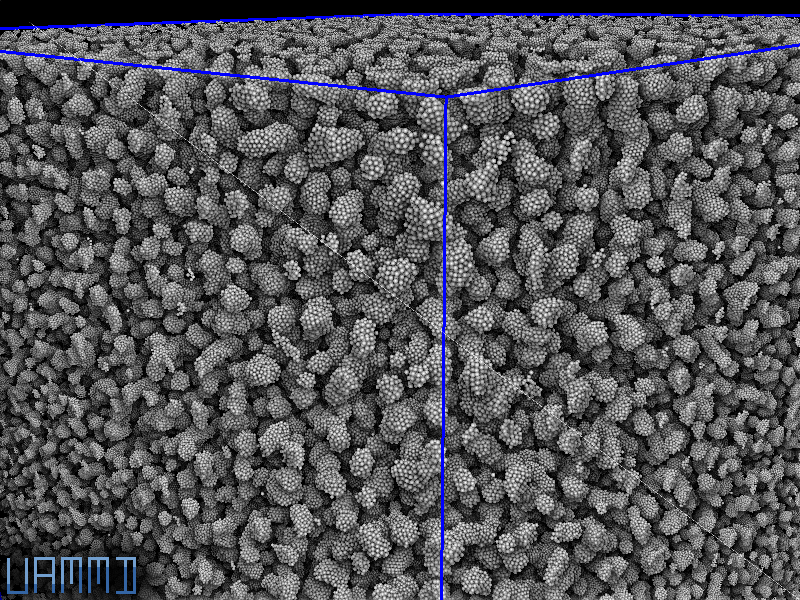
\includegraphics[width=\textwidth]{gfx/shotlogo}
  \caption{A screenshot of a \gls{LJ} fluid quenched to a low temperature made with superpunto. The simulation contains $10$ million particles, which are being rendered to the screen at about 30 frames per second in a GTX 980 \gpu.}
\end{figure}

\begin{itemize}
\item Superpunto, a particle visualizator.
\item Explain the need for a fast particle visualizer with a super simple format and pipe capabilities. Real time visualization using the pipe.
  
\end{itemize}

\section{Format}
inputfile should have the following structure:
\begin{minted}{\ucpp}
#Lx=X;Ly=Y;Lz=Z; Comments are used to separate frames, you can force the size of the simulation box starting the comment as in this example. All three L must be provided
X1 Y1 Z1 r1 c1 Vx Vy Vz#You can comment here aswell! If your file has more than
X2 ...         #8 columns, the rest will be ignored!
.
.
.
\# frame=2
X1 Y1 Z1 r1 c1 Vx Vy Vz
.
.
.
\# frame = 3
\end{minted}

\section{Graphical Techniques}

\begin{itemize}
\item Instanced drawing with OpenGL 4.5
\item The G-buffer technique
\item Lighting model.
\item Screen space ambient oclussion (SSAO).
\end{itemize}

\section{Controls}

\begin{itemize}
\item  Movement:
  \begin{itemize}
  \item Move with WASD, E and Q to tilt and Shift/Ctrl to go up/Down
  \item Use +/- to increase/decrease the speed
  \item Look around holding ALT and moving the mouse
  \item Rotate the world in XYZ using 123/456    
  \end{itemize}
\item Frame control:
  \begin{itemize}
  \item Press Space to go to the next frame, R to the previous
  \item Press T to go to the last frame, B takes you to the first one
  \item Press M to play the frames at 60 FPS, M again to pause
  \item Press C to take a screenshot in png
  \item Press L to play and record to a mp4 until L is pressed again
  \end{itemize}
\end{itemize}
\subsection*{Options}
\begin{itemize}
\item --record :  Makes a movie of all the frames in file and generates a .mp4
\item --frames-between-screenshots X : Number of frames skipped between screenshots when recording (default = 2)
\item --background R G B : Background color in RGB, default R=G=B=0.0
\item --palette X : Change the color palette
\item --RGB : Read colors as hex values in BGR (as integers) (0xFF=red=255). Overrides palette
\item --nobox : Do not render the bounding box.
\item --noaxis : Do not render axis labels.
\item --resolution X Y : Set the resolution (AKA window size). Default is 800x800          
\end{itemize}


\newpage
\cleardoublepage
\part{New physics and applications}\label{pt:applications}
\chapter{Measuring intracellular viscosity}

Using \gls{PSE} to model the environment of a cell. In particular how the presence of microtubulae affects the viscosity measured by a marker.

\chapter{Star Polymer dynamics in shear flow}
Using \gls{BDHI} via Cholesky to compute different properties of a low density solution of star polymers in shear flow.
% \chapter{Optofluidic Control of nanoscale dumbbells}

\chapter{Applications: Hydrodynamics in confined geometries}
\begin{itemize}
\item Long time self diffussion
\item Linear response theory for MSD
\item Ensemble averages for color
\item giant fluctuations comparison BD, q2D, t2D
\item Bridging the gap to 3D, the short time collective diffusion coefficient and the hydrodynamic function
\item Mention steric repulsion, only affects large wavenumbers (steric repulsion size), but the colective effect remains.
\end{itemize}
Bulk diffusion of particles in liquids is well-known to be controlled by hydrodynamics, and diffusion on interfaces is no exception. While the diffusion of colloids and polymers on a fluid-fluid interface has been studied theoretically since the 1970s \cite{FluidFluidInterface_Polymers,Diffusion2D_TwoViscosities}, \emph{collective diffusion} in a monolayer of colloidal particles confined to a fluid-fluid interface has only recently been explored in some detail both theoretically \cite{Bleibel2014,Bleibel2016,Bleibel2015} and experimentally[11].

The hydrodynamic coupling between the confining force acting on each individual colloid and their collective motion leads to surprising effects.
For instance, if the constraint is holonomic (colloids are restricted to move on a purely 2D domain), the confining force can be seen to arise from the non-zero divergence of the mobility tensor, which is related to the reduction of entropy imposed across the confining plane. In the case of a point wise force in unbounded fluid such flow perturbation (Oseen) decays like the inverse of the distance and, as a consequence, the diffusion coefficient of larger and larger colloidal density fluctuations increases without bounds. In particular, this results in the short-time collective diffusion diverging as the inverse of the wave number.
This unexpected finding has prompted re-examination of previous experimental results \cite{Diffusion2D_Experiments_Weitz,SD_TwoWalls,Diffusion2D_Experiments_Rice}, and it is plausible that the effect may have been overlooked in a number of other prior experimental and theoretical works as well.

The physical origin of the anomalous collective diffusion has already been elucidated in prior work by others\cite{Bleibel2014,Bleibel2016,Bleibel2015,Dominguez2014}. Basically, momentum conservation implies that the confining force acting on each particle has to propagate to the surrounding, incompressible, solvent. In the plane, the resulting hydrodynamic drag created by one particle acts like a flow source that induces an effective repulsive force on the other particles.

This results in strong displacement correlations which are the origin of the anomalous collective diffusion.
A new interpretation of this phenomena is obtained if one focuses on the in-plane dynamics.
In the plane, the field of diffusive displacements appears to be compressible due to the momentum source associated with each confined particle.
In the limit of strict confinement, the flow acts as a compressible two-dimensional cut through an incompressible three-dimensional flow field.
Because of this apparent compressibility, the Brownian motion of the particles creates an osmotic pressure proportional to $\kT$, which propagates via the fluid inducing long-ranged repulsive interactions.
This long-ranged repulsion decays slowly with the particle-particle distance, and dramatically accelerates collective diffusion at large scales.
Furthermore,
% contrary to what was previously thought \cite{Pelaez2017,Bleibel2017},
these long-ranged correlations also appreciably modify the single-particle diffusion, as we will see in future sections.

Such types of hydrodynamic enhancements do not only take place when the fluid is unbounded in the three directions. The presence of distant boundaries modifies the propagation (e.g., $1/r^2$ inside a slit channel[12,13]), leading to yet-unexplained and stronger variations of this phenomena which might also depend on the wall's slip boundary conditions.
We will study how this anomalous collective diffusion becomes normal as the confinement is made softer.

During the following chapters, we will study the collective diffusion and transport properties of a suspension of particles confined to a plane in two regimes:
\begin{itemize}
\item When the confinement is not strict and particles can leave the plane. For this, we can make use of the \gls{FIB} or \gls{FCM} described in previous sections and impose an external confining force on each particle. Although our implementations for these algorithms are triply periodic, we will neglect the contributions of the periodic copies of the system in the third direction by making the domain be much larger than the typical width of the suspension. We can also study the transient to the inertial regime by using \gls{ICM}.
\item In the limit of strict confinement. Since our region of interest is the purely 2D plane in which particles diffuse, we will develop a new algorithm that takes into account the unbounded fluid in the $z$ direction implicitly.
\end{itemize}
Additionally, we will describe a new doubly periodic algorithm capable of solving hydrodynamics in the first scenario by directly imposing a different set of boundary conditions at the domain limits in the third direction. In particular, we can use this new framework to impose open boundaries, with the possibility of adding one or two walls at the domain limits (particles near a wall or a slit channel).


%\chapter{Diffusion under soft confinement}\label{ch:softq2D}
We will see how this length scale governs the collective intermediate scattering function of colloids under harmonic confinement. We will examine how the enhancement of the collective diffussion dissapears going from the limit of strict confinement with $K_s\rightarrow \infty$ to the purely open 3D hydrodynamics with $K_s\rightarrow 0$.
Excluded volume and other potential interactions between colloids add another length scale to the collective diffusion, which partially masks the anomalous hydrodynamic enhancement. This masking depends on the static structure factor, $S(k)$, and here we illustrate the case of repulsive, \gls{WCA}, and attractive, \gls{LJ}, potentials.

Later, we will take the mathematical limit of $K_s\rightarrow \infty$ to connect 

%% Q2d paper intro:

%Previous work on collective diffusion of colloids on fluid-fluid interfaces\cite{Bleibel2014,Bleibel2016,Bleibel2015} has focused on the \emph{ensemble average}. Our focus here is on the \emph{fluctuations} around the ensemble average, i.e., on the equations for the evolution of a particular \emph{instance} (trajectory) of diffusive processes on interfaces. We use the fluctuating DDFT-HI developed in \cite{Donev2014}, which is closely-related to \emph{fluctuating hydrodynamics} (FHD)\cite{Donev2014_2}. The (formal) nonlinear equations of FHD are challenging to interpret \cite{SPDE_Diffusion_DDFT,DDFT_Hydro}, but, at the same time, they are more physically transparent than the ensemble-averaged equations, and do not require closures for noninteracting particles\cite{DDFT_Hydro}. Furthermore, as we will see later, the fluctuating DDFT-HI equations are a very useful tool for constructing linear-time Brownian Dynamics (BD) algorithms.
%%%%%%%


\begin{itemize}
\item Short time Collective diffusion
\item Recovering 3D Hydrodynamics
\item Color density fluctuations
  Understanding the magnitude and the dynamics of density fluctuations is crucial for several reasons. First, in actual experiments one observes individual instances, not the ensemble average. While in many systems typical instances are quite similar to the average, i.e., the fluctuations are small compared to the mean, this is not always the case. It is well-known that nonequilibrium fluctuations in diffusive processes are, rather generally, much larger in magnitude than equilibrium fluctuations, and are also long ranged \cite{FluctHydroNonEq_Book}.
Experiments in microgravity have measured these ``giant fluctuations'' in three dimensions, and shown that nonequilibrium diffusive fluctuations are correlated over macroscopic distances \cite{FractalDiffusion_Microgravity,GRADFLEXTransient}.

For diffusion in two-dimensional systems such as thin smectic films in vacuum \cite{ThinFilms_True2D}, linearized FHD predicts that the magnitude of the nonequilibrium fluctuations becomes comparable to the mean \cite{GiantFluctuations_ThinFilms}. The appearance of such ``colossal fluctuations'' implies that the ensemble average is no longer informative, since each instance looks very different from the mean.
It is therefore essential to understand whether individual instances of diffusive mixing processes on fluid-fluid interfaces evolve similarly to the ensemble average.
Second, fluctuations can be measured in experiments and reveal information about the underlying microscopic mechanism of diffusion. For diffusion in bulk three-dimensional liquids or in truly two-dimensional liquids (e.g., a hard-disk fluid), the ensemble average strictly follows the familiar Fick's law \cite{DiffusionJSTAT}.
This means that the ensemble-averaged concentration in a system where the diffusing particles are strongly correlated by hydrodynamics (e.g., two-dimensional thin smectic films \cite{ThinFilms_HIs}), will look indistinguishable from the ensemble average in a system where the diffusing particles are uncorrelated (e.g., diffusion in a solid).

But if one examines the magnitude of the nonequilibrium fluctuations, the hydrodynamic correlations are revealed through an unexpected power-law dependence of the structure factor on the wavenumber \cite{GiantFluctuations_ThinFilms}.

Third, collective fluctuations can couple bi-directionally to the motion of each particle and therefore \emph{renormalize} transport coefficients. For example, the fluctuating hydrodynamic theory developed in \cite{TracerDiffusion_Demery} shows that collective density fluctuations reduce the effective diffusion coefficient of a tagged particle in a dense system of uncorrelated Brownian soft spheres.
In this paper we will show that a similar effect exists even for an ideal gas of non-interacting but hydrodynamically-correlated particles diffusing on a fluid-fluid interface.

We will study the ensemble average and fluctuations of the density of spherical colloidal particles confined to diffuse on a fluid-fluid interface. We closely mimic the physical setting used in prior studies \cite{ConfinedDiffusion_2D,DDFT_Diffusion_2D,Diffusion2D_IdealGas}, and make a number of strong simplifying assumptions:
\begin{enumerate}
\item We assume that the interface is perfectly flat and that two fluids have the same viscosity; the case of unequal viscosity simply amounts to taking the arithmetic average of the two viscosities \cite{Diffusion2D_TwoViscosities,FluidFluidInterface_Polymers}.
\item In order to isolate the role of hydrodynamics from the role of other direct interactions such as capillary forces or steric/electrostatic repulsion, we focus on an \emph{ideal gas} of non-interacting spherical colloids \cite{Diffusion2D_IdealGas}.
  While such an idealized system could not be studied experimentally, it is a natural candidate for testing existing and developing new theories.
  Furthermore, light scattering observational data for colloids at a fluid interface support predictions made for an ideal gas of particles \cite{Diffusion2D_IdealGas}.
\item We assume that the colloids are strictly confined to the interface by a strong confining force in the $z$-direction, i.e., they cannot leave the $x-y$ plane.
  In reality, the confinement would be partial, for example, a laser sheet may provide a harmonic confining potential in the $z$ direction. However, prior work \cite{PartiallyConfined_Quasi2D,PartiallyConfinedDiffusion_2D} has shown that partial confinement only changes the results for larger wavenumbers (i.e., for wavelengths smaller than or comparable to the range of movement in the $z$ direction), and does not affect the anomalous diffusion in the plane.
  At the same time, we will show here that the case of strict confinement can be simulated much more efficiently using a two-dimensional Brownian dynamics algorithm.
\item We use a minimal far-field description of the hydrodynamics, as used in prior work by others \cite{ConfinedDiffusion_2D,DDFT_Diffusion_2D,Diffusion2D_IdealGas}.
Such a Rotne-Prager approximation is quantitatively accurate only for dilute suspensions, and we may question its usefulness in studying a \emph{collective }effect that is dominant at larger packing densities.
Nevertheless, as already mentioned, the anomalous collective diffusion arises because of a long-ranged (far-field) repulsion $\sim k_{B}T$.
We therefore believe that short-ranged (near-field) corrections to the hydrodynamics will not qualitatively change the phenomena studied here.
\end{enumerate}
While our focus is diffusion on a fluid-fluid interface, which we will refer to as Quasi2D (abbreviated q2D) diffusion, we will contrast Quasi2D diffusion to diffusion in truly two-dimensional systems such as thin films in vacuum \cite{ThinFilms_True2D}, which we will refer to as True2D (abbreviated t2D). Even though the diffusion is constrained to a two-dimensional plane in both cases, the hydrodynamics is essentially three-dimensional in Quasi2D but it is two-dimensional in True2D.
Our computational and analytical tools can easily be extended to other types of hydrodynamics. For example, it is believed that lateral diffusion in lipid membranes \cite{MembraneDiffusion_Review} or thin smectic films in air \cite{ThinFilms_HIs} can be described using a hydrodynamic model first proposed by Saffman. The (2+1)-dimensional ((2+1)D for short) Saffman model has already been combined with linearized fluctuating hydrodynamics in \cite{GiantFluctuations_ThinFilms}, but an experimental confirmation of the predictions of the theory is still lacking.

\end{itemize}




\begin{itemize}
\item Enhanced diffusion under soft confinement\cite{Pelaez2017}
\item Limit to infinetely stiff confinement\cite{Pelaez2018}
\item Describe quasi2D paper. Similar to \gls{FCM}, but with a Green's function that is integrated in Z. It is the limit of an infinite boxin Z with particles attached to z=0 via an infinitely stiff spring.
\end{itemize}



\part{Appendix}

\appendix

\chapter{Basic notions of CUDA/C++ programming}\label{sec:cpp}

\uammd uses the C++14 standard\footnote{The only restriction in adopting more modern standards, like C++20, is the adoption rate of CUDA. To the date of writing, the latest CUDA toolkit supports up to C++17.}, which presents subtle but sometimes important differences with the previous iteration of the language (C++11). Note however, that this standard is wildly different to ``classic'' C++98, which could be considered another language altogether. Furthermore, \uammd uses the CUDA extensions to the language, which introduce some new keywords and subtle rules.

In this chapter, we will give a few hints to ease the interpretation of the code examples throughout this manuscript for the uninitiated. Note that this is not intended to be a thorough description or tutorial of the language. For that the reader is redirected to the plethora of resources available online regarding CUDA and modern C++. This chapter summarizes the bare minimum necessary for a reader to follow the logic in the examples scattered throughout this manuscript.

CUDA/C++ is a compiled language, meaning that before executing a source code, it must be transformed into an executable binary by an external program called the \emph{compiler}. We will also refrain from discussing the compilation of CUDA codes\footnote{\uammd's online resources shed light into this process, which might change over time for reasons outside of the author control.}.

Lets start with some basic concepts in C++ and then go to the \gpu. The entry point for execution in all C++ codes starts with a function called ``main''. This function must be defined by the user with the name ``main'' and a returning type int (see example code \ref{code:minimal}).

\begin{code2}[A C++ program that does nothing.]
{label=code:minimal}
//This is a comment, which is ignored by the compiler
//The main function must be present in all C++ programs
int main(){
  //main must return an integer, encoded as 0 if the
  // program terminated sucessfully, and 1 otherwise.
  return 0;
}
\end{code2}

\subsection*{The auto keyword}
The keyword \emph{auto} can be seen in almost every code example in this manuscript. In contrast with other loosely typed languages, C++ forces the developer to always state the actual type of a variable when defining it. Similarly, the return type of a function must be specified.
In some situations, for instance when dealing with metaprogramming (which we will discuss shortly), knowing the name of the relevant type can become cumbersome and verbose. Luckily, the latest standards allow to replace the type name by the keyword \emph{auto}. When the compiler sees a variable with the type \emph{auto}, it will automatically deduce the correct type for it. Example code \ref{code:foo} introduces a couple of use cases for the \emph{auto} keyword.

\subsection*{Functions}
Main is an example of a function (albeit a special one), the syntax for defining custom functions is similar, see code \ref{code:foo}. The special return type \mintinline{\ucpp}{void} can be used to signify that a function returns nothing.

\begin{code2}[Defining a function in C++.] {label=code:foo}
//We can define a function with the syntax below
//The returning type, in this case int, can be replaced 
// by the keyword auto.
int foo(int a){
  //This function takes an integer, refered to as "a"
  // and returns its value multiplied by 2
  return a*2;
}
//The main function will simply call the foo function with an
// arbitrary number and store the result in a variable
int main(){
  int value = foo(12);
  //value holds the integer 24
  //The type of the variable, int, can be replaced by auto
  return 0;
}
\end{code2}

\subsection*{Including other codes}
By default, a C++ source code will have access only to the basic rules of the languages. We can add libraries via the \emph{include} directive, which will make available to us every function, class an variable defined in another file. For instance, in example code \ref{code:hello} we can see how to include the standard library header file that provides printing functionality.

\begin{code2}[The classic Hello World program in C++. Once executed, it will print ``Hello world'' to the terminal.] {label=code:hello}
  #include<iostream> //Includes std::cout and std::endl
  //Uncommenting the line below permits to omit
  // the std::
  //using namespace std;
  int main(){    
    std::cout<<"Hello world"<<std::endl;    
    return 0;  
  }
\end{code2}

\subsection*{Namespaces and the using keyword}
In order to avoid naming collisions (two libraries or files defining entities with the same name) C++ provides the concept of \emph{namespaces}. We have already seen the standard library namespace, \emph{std}, in action in example \ref{code:hello}. In order to reference an entity inside a given namespace, the ``::'' operator is used. In the aforementioned example, we access the object \emph{cout} of the \emph{std} namespace with \mintinline{\ucpp}{std::cout}.

This can become a nuissance when a given namespace is constantly used. C++ provides the \mintinline{\ucpp}{using namespace} construct to mitigate this. For instance, throughout this manuscript, the line \mintinline{\ucpp}{using namespace uammd;} is used to omit writting \mintinline{\ucpp}{uammd::} every time an \uammd entity is referenced.

The \mintinline{\ucpp}{using} keyword has a second usage, it allows to ``rename'' a type. In C++ type names can become quite convoluted and long. The \mintinline{\ucpp}{using} keyword can be used in these cases. For instance, in example code \ref{code:pf} we write the line \mintinline{\ucpp}{using PF = PairForces<Potential, NeighbourList>;}, allowing to use simply ``PF'' when we want to refer to the longer type name.
\subsection*{Objects}
Although C++ can work as a functional language, it is heavily object oriented. The \mintinline{\ucpp}{struct} and \mintinline{\ucpp}{class} keywords are used to define objects in C++\footnote{The only difference between a struct and a class is the default visibility of its members. By default, members in a struct have public visibility, whereas a class defaults to private visibility.}.

An object can hold both variables and functions, which are refered to as \emph{members}. A member function in a class has access to all other members of the object.

In the author's personal programming style, structs are usually used to serve as an aggregate of variables, whereas classes are used as a more complex object (with member functions, etc). Note however, that the struct and class keywords are almost interchangeable.

\begin{code2}[Examples of object creation.] {label=code:class}
  #include<iostream>
  //The syntax for creating a struct with type name Parameters, holds two double variables.
  struct Parameters{
    double var1;
    double var2;    
  };
  //A class with public visibility is equivalent to a struct.
  class MyClass{
    //The public keyword marks every defined member below as accessible from outside
    public:
    void print(){
      std::cout<<"Hello"<<std::endl;
    }
  };
  int main(){
    //Create an instance of the struct Parameters
    Parameters par;
    //Set the value of one of its variables
    par.var1 = 1.0;
    //Create an instance of the object MyClass
    MyClass c;
    //Call it's member "print".
    c.print();
    return 0;  
  }
\end{code2}
Given that object can be created and passed around as regular variables, we can use them to encapsulate and transport logic between different parts of the code.

In \uammd, every \emph{Interactor} and \emph{Integrator} is provided as a C++ \mintinline{\ucpp}{class}.


\subsection*{Object inheritance}
In C++, objects can inherit the functionality of other classes, and even override some of it. For instance, every polygon has an area, we can create a class called \emph{Polygon} that provides a member function called \emph{area} (returning the area). However, a polygon is just a concept that has no area per se. We can then create another class called \emph{Square} that inherits from \emph{Polygon} and overrides the \emph{area} function, providing its squared side.

Given that the area of a \emph{Polygon} object is meaningless, we can mark it's \emph{area} function as \mintinline{\ucpp}{virtual} and add the suffix \mintinline{\ucpp}{= 0;} to its signature. This transforms the \emph{Polygon} class into a \emph{virtual base class}, which means that it cannot be instanced directly, rather it must be inherited and the virtual members must be overriden. See example code \ref{code:inherit}.
\begin{code2}[Inheriting a virtual class.] {label=code:inherit}
  //This is a virtual class
  class Polygon{
    public:
    virtual double area() = 0;
  };
  //This class is a kind of Polygon (inherits from it)
  class Square: public Polygon{
    double side = 2.0; //An arbitrary value for the side
    public:
    //We can override the area member of Polygon
    virtual double area() override{
      return side*side;
    }
  };
  //This class is a kind of Polygon (inherits from it)
  class Circle: public Polygon{
    double radius = 2.0; //An arbitrary value for the radius
    public:
    //We can override the area member of Polygon
    virtual double area() override{
      return 3.1415*radius*radius;
    }
  };

  int main(){
    Square s;
    auto a = s.area();
    Circle c;
    auto a2 = c.area();
    return 0;  
  }
\end{code2}

In \uammd, \emph{Interactor} and \emph{Integrator} are virtual classes such as \emph{Polygon}. One of the benefits of using inheritance is that it allows to provide a general logical interface. In general C++ an inherited class can mascarade as an instance of the parent class (but not the other way around). So a \emph{Square} can be used as a \emph{Polygon} but not viceversa. This only happens, however, for pointers (since the virtual base class cannot be instanced directly).

Let us discuss now the type of pointer used throughout this manuscript, the \mintinline{\ucpp}{std::shared_ptr}.

\subsection*{Shared pointers}
Without going into detail (the reader can learn more online), a C++ shared pointer can hold ownership of an object through a pointer. In the \uammd examples in this manuscript we use shared pointers mainly to pass around \emph{Interactors} and \emph{Integrators}. For instance, in example \ref{code:pf} we create and return an instance of \emph{PairForces}, a class inherited from \emph{Interactor}. On the other hand, the \emph{Integrator} member function \mintinline{\ucpp}{addInteractor();} will take in its argument a pointer to an \emph{Interactor}, meaning that the \emph{PairForces} instance created in example \ref{code:pf} can be passed to an \emph{Integrator} (such as the one created in example \ref{code:md}) directly.


\begin{code2}[Using shared pointer to hold many types of polygons.] {label=code:sharedptr}
  #include<memory> //std::shared_ptr
  #include<vector> //std::vector
  //Using the Polygon declarations of the previous example
  //This function takes a pointer to a polygon and returns its area
  auto getAreaOf(std::shared_ptr<Polygon> pol){
    return pol->area();
  }
  int main(){
    //Create pointers to a square and a circle
    auto s = std::make_shared<Square>();
    auto c = std::make_shared<Circle>();
    //The getAreaOf function works for pointers of any class that inherits from Polygon
    double as = getAreaOf(s);
    double ac = getAreaOf(c);
    //We can also aggregate pointers to Polygon childs in a vector
    std::vector<std::shared_ptr<Polygon> > vec({s, c});
    return 0;  
  }
\end{code2}

\subsection*{Metaprogramming}
In addition of inheritance, C++ offers another way of writing generic code called templates. A template is a function or object that is generic for any type (sometimes the type is restricted under some assumptions). For instance, let us rewrite the function \mintinline{\ucpp}{getAreaOf} in example \ref{code:sharedptr} using metaprogramming instead of inheritance.

\begin{code2}[Using shared pointer to hold many types of polygons.] {label=code:sharedptr}
  //This function takes any type and returns its area. Of course, it will not compile if the provided type has no member function called area.
  //When we call this function, T will be replaced by the type of the provided argument
  template<class T>
  auto getAreaOf(T pol){
    return pol.area();
  }
  int main(){
    Square s;
    Circle c;
    //The getAreaOf function now works any type that provides a function called
    // area
    double as = getAreaOf(s);
    double ac = getAreaOf(c);    
    double var = 1.0;
    //The code would be invalid if a double is passed, since the function expects the member area to exists.
    //double avar = getAreaOf(var);
    return 0;  
  }
\end{code2}

In \uammd, templates are used extensively to generalize modules. For instance, the \emph{PairForces} module (see example code \ref{code:pf}) is templated for both the potential and the neighbour list.



\subsection*{Other keywords}
The \mintinline{\ucpp}{const} keyword simply informs the reader (and compiler) that the value of the accompanying variable cannot be modified after its declaration. When appearing in the signature of an object's member function, it conveys that the function will not modify the state of the object in any way.


\section{Basic concepts of GPU programming}
Things to explain here:

\begin{itemize}
\item Separation between CPU and GPU RAM
\item Different memories in the GPU; global memory, register memory, shared memory, constant memory.
\item Threading model; blocks and threads per block
\item Execution order of threads (threads execute in lock-step inside a warp), blocks are async between them.
\item Concurrent threads like to access concurrent elements in memory.
\end{itemize}



\chapter{Dealing with the FFT in the GPU} \label{ch:appendixa}

Many of the numerical techniques in this manuscript make use of the \gls{FFT}, mostly in order to easily compute convolutions. The \gpu is a very powerful hardware for \gls{FFT}, but using the available \glspl{API} can become a real nuisance. In this chapter we will see how \uammd makes use of the CUDA library \emph{cuFFT}\cite{cufft} and how to work with data in Fourier space. While the information hereafter is centric to the \emph{cuFFT} library, most lessons are applicable to other popular \gls{FFT} libraries (such as \emph{FFTW}).
The documentation of the \emph{cuFFT} library is sometimes obscure (and even lacking). There are some particular details that have made me waste countless hours, hopefully with the help of this chapter you can spare some.

Lets assume we want to work on some three dimensional data defined on the nodes (cells) of a mesh (grid) with size $\vec{n} = (n_x, n_y, n_z)$. For instance, the forces spreaded to the grid in \gls{FCM}.
A one dimensional transform has size $(n: = \vec{n} =(n_x,1,1)$.

We will store the data in a linear array of size $n_xn_yn_z$, and access the value of cell $\vec{c} = (c_x,c_y,c_z)$ at the element $i = c_x + (c_y + c_zn_y)n_x$. Where $c_{x/y/z} \in [0, n_{x/y/z}-1]$.

\section*{Choosing an efficient grid size}
\gls{FFT} libraries will typically process transformations of any sizes, however, many algorithms are dramatically more efficient when the size meets some conditions. Often the most efficient transform sizes are the powers of two ($n = 2^i$), but in general a multiple of the first prime numbers will work as well

\begin{equation}
  \label{eq:fftfriendly}
n = 2^i3^j5^k7^l11^m
\end{equation}

Where $i,j,k,l,m$ are integer numbers. A number that meets that can be expressed like this is refered to as an \gls{FFT}-friendly number.
Typically we will look for the next friendly number given a certain target size. One way to find this number is to simply generate all numbers that meet eq. \eqref{eq:fftfriendly}, sort them and find the nearest one to a target.

Although this is a good rule of thumb, we can expect the performance to vary between implementations, hardware and version. The best strategy is to test in a case by case basis. This can be worth for long simulations, since this means that a bigger transformation can sometimes be faster. Given that in many spectral algorithms a bigger grid size means more accuracy, we could get a more accurate run with a shorter runtime.


\section*{Complex to real (C2R) and Real to complex (R2C) transforms}

One particular optimization commonly employed is to take advantage of the fact that, in a C2R or R2C transform, half the wave numbers are redundant. In these cases the signal in Fourier space, $\hat{s}(\vec{k})$, must meet that
\begin{equation}
  \hat{s}(\vec{k}) = \hat{s}(\vec{n} - \vec{k})^*
\end{equation}
In particular \emph{cuFFT} will only store the first $\textrm{floor}(n/2)+1$ wavenumbers in the $x$ direction. By default, a R2C transform will take an input of size $\vec{n}$ real numbers and return a complex array of size $\hat{\vec{n}} := (\textrm{floor}(n_x/2)+1, n_y, n_z)$ complex numbers\footnote{Note that since a complex number is stored as of two real numbers, the storage of both arrays is equal}. Similarly, a C2R transform will take a $\hat{\vec{n}}$ sized complex array and return a size $\vec{n}$ array with real numbers.

In principle, \emph{cuFFT} allows to store the input and output of a C2R or R2C transform in the same array in what it's called an \emph{in-place} transform. However, in my experience this results in unexpected behavior, so I advise against it\footnote{The documentation hints that in these cases the input size in the $x$ direction for an in-place C2R transform should be $2(\textrm{floor}(n_x/2)+1)$ to accomodate for all necessary complex values in the output. However, this does not seem to be the same rule for a C2R transform and has caused some problems to me in the past}.

\section*{Data layout}
Since most spectral algorithms in \uammd require C2R and R2C transforms it is worth giving here some more details about the correspondence of wave numbers and elements in the data array.

Here is a convenience function that returns the wave number that corresponds to a certain index in the data array.
\begin{code2}[Getting the wave number corresponding to a given linearized index.]{label=code:i2wn}
int3 indexToWaveNumber(int i, int3 nk){
  int ikx = i%(nk.x/2+1);
  int iky = (i/(nk.x/2+1))%nk.y;
  int ikz = i/((nk.x/2+1)*nk.y);
  ikx -= nk.x*(ikx >= (nk.x/2+1));
  iky -= nk.y*(iky >= (nk.y/2+1));
  ikz -= nk.z*(ikz >= (nk.z/2+1));
  return make_int3(ikx, iky, ikz);
}
\end{code2}

Most \gls{FFT} libraries povide some kind of advanced interface allowing to customize the data layout to some extent. In \emph{cuFFT} this is called the \emph{Advanced Data Layout}. In \uammd this is used extensively to compute three or four transformations in a single batch using interleaved data. For example, we can directly transform the forces spreaded to the grid in \gls{FCM} (see sec. \ref{sec:fcm}) stored in a vector \emph{real3} elements.
For example, if we want to transform the three coordinates for the forces in an interleaved array, we can instruct the library to interpret this data as three signals, each starting after the other and strided by three elements.
\section*{Nyquist points}
In a complex to real transform (and thus also in a real to complex transform) the corresponding Fourier data points meet the conditoin $data(\vec{k}) = data(\vec{k} - \vec{n_k})^*$. A consequence of this is that, in a transformation with an even number of points in some direction, there are some points that are the conjugates of themselves. We call this uncoupled modes Nyquist points.
There are $8$ nyquist points at most (including the $\vec{k} = (0,0,0)$ mode), corresponding to the vertices of the inferior left cuadrant.
A function to determine if a certain wave number is a Nyquist point:
\begin{code2}[Finding Nyquist numbers]{label=code:nyquist}
bool isNyquistWaveNumber(int3 ik, int3 n){
  //Is the current wave number a nyquist point?
  const bool isXnyquist = (ik.x == n.x - ik.x);
  const bool isYnyquist = (ik.y == n.y - ik.y);
  const bool isZnyquist = (ik.z == n.z - ik.z);
  const bool nyquist =  
    (isXnyquist and ik.y==0    and ik.z==0)    or //1
    (isXnyquist and isYnyquist and ik.z==0)    or //2
    (ik.x==0    and isYnyquist and ik.z==0)    or //3
    (isXnyquist and ik.y==0    and isZnyquist) or //4
    (ik.x==0    and ik.y==0    and isZnyquist) or //5
    (ik.x==0    and isYnyquist and isZnyquist) or //6
    (isXnyquist and isYnyquist and isZnyquist);   //7
  return nyquist;
}
\end{code2}


\chapter{Boundary Value Problem (BVP) Solver} \label{sec:bvp}
In sections \ref{sec:dpstokes} and \ref{sec:dppoisson} we laid out the basic \glspl{PDE} as \glspl{BVP} with the following generic form
\begin{equation}
  \label{eq:bvpmain}
  \begin{aligned}
    &(\partial_{zz}-k^2)y(z)=f(z)\\
    &(\partial_{z}\pm k)y(\pm 1)=
    \begin{bmatrix}
      \alpha\\
      \beta
    \end{bmatrix}
\end{aligned}
\end{equation}
Where $\partial_z y:= \frac{\partial y}{\partial z} := y'(z)$ and $\partial_{zz} y:= \frac{\partial^2 y}{\partial z^2} := y''(z)$
%\begin{equation}
%  \label{eq:bvpmain}
%  \begin{aligned}
%    &y''(z)-k^2y(z)=f(z)\\
%    &y'(1)+ ky(1)=\alpha ,\qquad y'(-1)- ky(-1)=\beta.
%\end{aligned}
% \end{equation}

The domain is here defined in the $[-1, 1]$ range for simplicity. We can later generalize to any size via a simple change in units. In particular by defining $z = z'/H$ (with $z'\in [-H, H]$) and $k = k'H$.

In this section we describe a generic, \gpu-friendly, spectral solver for the set of equations in \eqref{eq:bvpmain} based on the spectral integration method described in\cite{Greengard1991}.


We will work with the discrete Chebyshev transform of eq. \eqref{eq:bvpmain}. In general, we can expand a given function, $g(z)$ with $z\in \mathcal{R}$ into the first $N$ terms of its Chebyshev series so that
\begin{equation}
\label{eq:bvpchebexp}
g(z) = \sum_{n=0}^{N-1} \fou{g}_n T_n(z)
\end{equation}
Where we use the subscript $n$ to distinghuish between the Chebyshev and Fourier coefficients (since throughout this manuscript we have used the subscript $k$ to denote Fourier coefficients).

In general, the Chebyshev polynomials of the first kind, $T_n$, are defined via a recurrent relation with
\begin{equation}
  \label{eq:bvpchebpoly}
  \begin{aligned}
    T_0(x) &= 1\\
    T_1(x) &= x\\
    T_{n+1}(x) &= 2xT_n(x) - T_{n-1}(x)
  \end{aligned}
\end{equation}

On the other hand, the Chebyshev polynomials can be interpreted as a cosine series under a change of variables. Given that by definition $T_n(cos(\theta))= cos(n\theta)$, evaluating the function at the extrema points $x_n = cos(n\pi/(N-1))$ transforms the expansion in eq. \eqref{eq:bvpchebexp} into a cosine series. We can then leverage the \gls{FFT} to perform a discrete cosine transform by transforming the periodic extension of a signal. This allows to obtain the Chebyshev coefficients of a signal in $O(Nlog(N))$ operations. We refer to this technique as the \gls{FCT} (see chapter 8 of \cite{Trefethen2000}). In Appendix \ref{sec:fct} we give some details about how to do this in a computer implementation.

We can then leverage several interesting properties of the Chebyshev series to easily (and exactly) derivate and integrate the different quantities.

%If we evaluate $f(z)$ in the roots of the Chebyshev polynomials, $z_i=cos(i\pi/N)$, we can leverage the \gls{FFT} to provide the coefficients of the Chebyshev transform (in what is usually refered to as a Fast Chebyshev Transform (FCT)) by using it to compute a discrete cosine transform. The proof, while straight forward, is cumbersome and beyond the scope of this work, it can be found in Chapter 8 of\cite{Trefethen2000}. In particular, the fast Chebyshev transform is carried out by taking the \gls{FFT} of the periodic extension of $f(z)$\footnote{cuFFT can be used for this, which is the approach in \uammd.} 

In particular, we can use the well known indefinite integrals of the Chebyshev polynomials to integrate $\fou{y}''_n$ twice and get $\fou{y}_n$. First by integrating $\fou{y}''_n$:
\begin{equation}
  \begin{aligned}
\fou{y}'_1&= \frac{1}{2}\left(2\fou{y}''_0-\fou{y}''_2\right)\\
\fou{y}'_n &= \frac{1}{2n}\left(\fou{y}''_{n-1}-\fou{y}''_{n+1}\right), \quad n \geq 1.
\end{aligned}
\end{equation}
%Eq. \eqref{eq:ds} is the relationship used to apply the Chebyshev differentiation matrix in linear time to compute $\displaystyle \frac{\partial \hat{f}^z}{\partial z}$ in Eq.\ \eqref{eq:bvp_p}. Specifically, we set $d_{N-1}=0$ and can then compute $a_n$ for all $n=N-1, \dots 0$ (in that order).  
And then integrating again
\begin{equation}
  \label{eq:bvpyn}
  \begin{aligned}
&\fou{y}_1 = \frac{1}{2}\left(2\fou{y}'_0-\fou{y}'_2\right)=\fou{y}'_0 -\frac{1}{8}\left(\fou{y}''_1-\fou{y}''_3\right)\\
&\fou{y}_2 = \frac{1}{4}\left(\fou{y}'_1-\fou{y}'_3\right)=\frac{1}{4}\left[\frac{1}{2}\left(2\fou{y}''_0-\fou{y}''_2\right)-\frac{1}{6}\left(\fou{y}''_2-\fou{y}''_4\right) \right]\\
&\fou{y}_n = \frac{1}{2n}\left(\fou{y}'_{n-1}-\fou{y}'_{n+1}\right)=\\
&\quad\quad\frac{1}{2n}\left[\frac{1}{2n-2}\left(\fou{y}''_{n-2}-\fou{y}''_n\right)-\frac{1}{2n+2}\left(\fou{y}''_n-\fou{y}''_{n+2}\right) \right], \quad n \geq 3.
\end{aligned}
\end{equation}
This formulation gives two free parameters $\fou{y}_0$ and $\fou{y}'_0$, which are obtained using the \glspl{BC}. Additionally, we consider $\fou{y}''_n = \fou{y}'_n = 0$ for $n > N-1$ when calculating $\fou{y}_n$ using \eqref{eq:bvpyn}.

Now, we can reformulate the boundary value problem using the Chebyshev series representations in \eqref{eq:bvpchebexp} as
\begin{equation}
\label{eq:bvpn0}
\sum_{n=0}^{N-1} (\fou{y}''_n-k^2\fou{y}_n)T_n(z) = \sum_{n=0}^{N-1}\fou{f}_n T_n(z).
\end{equation}
Matching modes gives a system of $N+2$ equations for the Chebyshev coefficients
\begin{equation}
\label{eq:bvpmodes}
\begin{aligned}
&\fou{y}''_n-k^2\fou{y}_n=\fou{f}_n \qquad n=0, \dots, N-1\\
&\sum_{n=0}^{N-1} (\fou{y}'_n+k\fou{y}_n) = \alpha\\
&\sum_{n=0}^{N-1} (\fou{y}'_n-k\fou{y}_n) (-1)^n = \beta
\end{aligned}
\end{equation}
Where has $N+2$ unknowns $\fou{y}_0, \fou{y}'_0, \fou{y}''_0, \dots \fou{y}''_{N-1}$. We solve the algebraic system of equations\ \eqref{eq:bvpmodes} for the second derivative coefficients $\fou{y}''_0, \dots \fou{y}''_{N-1}$ and integration constants $\fou{y}_0$ and $\fou{y}'_0$, then determine $\fou{y}_n$ by integrating twice using \eqref{eq:bvpyn}.

For the $k=0$ mode, the system reduces to the trivial system of equations
\begin{equation}
\label{eq:bvpmodes0}
\fou{y}''_n=\fou{f}_n \qquad n=0, \dots, N-1.
\end{equation}
The factors $\alpha$ and $\beta$, which in general can be different for each $k$, are zero for $k=0$, so in tfou case we enforce
\begin{equation}
\label{eq:bvpBCs0}
\sum_{n=0}^{N-1} \fou{y}_n = 0, \qquad \sum_{n=0}^{N-1} \fou{y}_n (-1)^n = 0.
\end{equation}

We use a Schur complement approach to solve the algebraic system of equations \eqref{eq:bvpmodes}. We can write the system in block form as 
\begin{equation}
\label{eq:blocksys}
\begin{pmatrix} \bm{A} & \bm{B} \\[2 pt] \bm{C} & \bm{D} \end{pmatrix}
\begin{pmatrix} \fou{\bm{y}}''\\ \fou{y}_0 \\ \fou{y}'_0 \\ \end{pmatrix}
= \begin{pmatrix}  \fou{\bm{f}}\\ \alpha \\ \beta\\ \end{pmatrix}. 
\end{equation}
Here $\bm{B}$ is $N \times 2$, $\bm{C}$ is $2 \times N$, $\bm{D}$ is $2 \times 2$, and $\bm{A}$ is an $N \times N$ \textit{pentadiagonal} matrix. In particular, the matrix $\bm{A}$, refered to as the second integral matrix, has only three non zero diagonals ($i=j$ and $i = j\pm 2$) which allows to use a specialized factorization algorithm. In \uammd we use the so-called \emph{KBPENTA} in \cite{Karawia2010}, modified for the special case of only three nonzero diagonals.\footnote{The matrix $\bm{A}$ is pre factorized (incurring an auxiliar storage of $3N$ elements for a given $k$). Using this our special pentadiagonal system can be solved in just $2N$ operations.} 

We then solve the $2 \times 2$ system
\begin{equation}
(\bm{C}\bm{A}^{-1}\bm{B}-\bm{D})\begin{pmatrix}  \fou{y}_0 \\ \fou{y}'_0\\ \end{pmatrix} = \bm{C}\bm{A}^{-1}\bm{f}-\begin{pmatrix}  \alpha \\ \beta\\ \end{pmatrix}
\end{equation}
for $\fou{y}_0$ and $\fou{y}'_0$. The $2\times 2$ matrix in the left hand side as well as $\bm{C}\bm{A}^{-1}$ ($2\times N$ size) are precomputed and stored for each $k$. Since the inverse of $\bm{A}$ is only needed at the precomputation stage no special performance considerations are required for it\footnote{In \uammd, the CPU \emph{getrf} BLAS square matrix inversion routine is used.}.

Finally we obtain the coefficients $\fou{\bm{y}}''=(\fou{y}''_0, \dots \fou{y}''_{N-1})$ by solving
\begin{equation}
\bm{A}\fou{\bm{y}}''=\left(\bm{f}-\bm{B}\begin{pmatrix}   \fou{y}_0 \\ \fou{y}'_0\\ \end{pmatrix}\right)
\end{equation}
using the pre-factorized modified \emph{KBPENTA} algorithm.

Note that we need to solve this system for each wave number, $k$. Our solver requires the evaluation of several recurrent relations, making it mostly a serial algorithm not worth parallelizing. In order to take advantage of the \gpu, we assign a thread to each $k$. As described above, much of the problem can be precomputed at the expense of memory storage (around $5N_kN$ values in total, being $N_k$ the number of wave vectors\footnote{Since we use R2C \gls{FFT} we will typically have $N_k=(N_x/2+1)N_y$.}
Except for the $k=0$ wave number, every solve is identical in operations, meaning that each thread will present the same memory access pattern in the, precomputed, auxiliar arrays. We take advantage of this by storing them in a coherent (strided) way, where a given element of an auxiliar array is stored contigously (and ordered) for all wave numbers (so that the thread access pattern is cache friendly)\footnote{I wrote a special \gpu auxiliar storage handler for this that allows to switch between a strided and contigous pattern. It can be found in the file \emph{BVPMemory.cuh} in \uammd. In general a strided access provides a much better performance.}. Testing suggests that our \gls{BVP} solver yields similar performance as the \gls{FCT} for small $N_k$, becoming increasingly faster for increasing $N_k$ (as expected given that our solver has linear scaling as opposed to the $O(Nlog(N))$ operation count of the \gls{FCT}).

\chapter{The Fast Chebyshev Transform}\label{sec:fct}

\begin{itemize}
\item Describe the FCT.
\item Its the FFT of the periodic extension of the signal evaluated at the Chebyshev roots
\item Numerical periodic extension is $F_{2N-i} = f_i$ where $i=1,2,...,N-1$.
\item Describe the numerical indexing intricacies and the scaling factors
\end{itemize}


\defbibheading{bibintoc}[\bibname]{%
  \phantomsection
  \manualmark
  \markboth{\spacedlowsmallcaps{#1}}{\spacedlowsmallcaps{#1}}%
  \addtocontents{toc}{\protect\vspace{\beforebibskip}}%
  \addcontentsline{toc}{chapter}{\tocEntry{#1}}%
  \chapter*{#1}%
}

\chapter{UAMMD's online documentation}\label{ch:online}
At the time of writing, the \uammd codebase is hosted as a git repository in the github platform (currently the de facto standard git hosting platform), at \url{https://github.com/RaulPPelaez/UAMMD}. Platforms change over time and github might not exist at the time you are reading this\footnote{As a side note, the \uammd was included among the github's Artic Code Vault program repositories. Thus, a physical copy of the codebase can be found 250 meters under the permafrost in a vault inside an abandoned coal mine in the Svalbard archipielago. This means that the codebase should be retrievable for at least the next thousand years.}. If that is the case and a google search does not help you locate its new hosting you have two options; either find me and request it directly or look in the wayback machine. At the time of writing, the internet archive has already scraped the uammd repository at least once, you can find the archived versions at \url{http://web.archive.org/web/202*/https://github.com/RaulPPelaez/UAMMD}.

This very manuscript is focused on the underlying theory behind the many algorithms exposed by the code as well as the design choices involved in its creation. However, it is not intended as an usage guide for \uammd (although several code examples are included). A user wanting to learn how to use \uammd can benefit from the online resources. In particular, \uammd offers three distinct sources of knowledge:
\begin{enumerate}
\item Code examples.
  The repository itself contains a plethora of organized usage examples showcasing the different \uammd's functionalities. In particular, the \emph{basic\_concepts} folder contains a series of tutorial-like examples intended as an introduction to the \uammd ecosystem.
\item Wiki.
  A wiki accompanying the codebase provides extensive information about all the available modules, as well as detailed information about the compilation process.
\item Marc's book, ``A Painless Introduction to Programming UAMMD Modules''\cite{Marc2020}.
  This book provides an introduction to \uammd from the very ground up, while making little assumptions about the readers familiarity with programming, complex fluids and their related numerical methods.
\end{enumerate}

\chapter{The Transverser and Potential interfaces}\label{ch:transverser}
\section{The Transverser Interface} \label{sec:transverser}
Many of the algorithms described in this manuscript require some kind of particle traversal.
%A Transverser is a concept that refers to the action of going through each element of something.  
Say, for instance, that for each particle we want to visit the rest of the particles that are closer than a certain distance. Or simply all of the other particles. More generally, we might want to perform some kind of operation equivalent to a matrix-vector multiplication, for which in order to compute one element of the result, the vector needs to go through a row of the matrix.
In these cases, a \emph{Transverser} is used.

A \emph{Transverser} holds information about what to do with a pair of particles, what information is needed to compute this interaction, and what to do when a particle has interacted with all pairs it is involved in.  

Being such a general concept, a \emph{Transverser} is used as a template argument, and therefore cannot be a base virtual class that can be inherited. This is why it is a "concept". No assumption can be made about the return types of each function, or the input parameters, the only common things are the function names.  

For each particle to be processed the \emph{Transverser} will be called for: \todo{Draw this in a skematik}
\begin{itemize}
\item Setting the initial value of the interaction result (function \emph{zero})
\item Fetching the necesary data to process a pair of particles  (function \emph{getInfo})
\item Compute the interaction between the particle  and each of its neighbours (function \emph{compute})
\item Accumulate/reduce  the result for each neighbour (function \emph{accumulate})
\item  Set/write/handle the accumulated result for all neighbours (function \emph{set})
 \end{itemize}
The same \emph{Transverser} instance will be used to process every particle in an arbitrary order. Therefore, the Transverser must not assume it is bound to a specific particle.

The \emph{Transverser} interface requires a given class/struct to provide the following public device (unless prepare that must be a host function) member functions:

\begin{itemize}
\item \mintinline[breaklines]{\ucpp}{Compute compute(real4 position_i, real4 position_j,Info info_i, Info info_j);}

  
  For a pair of particles
  characterized by position and info this function must return the
  result of the interaction for that pair of particles. The last
  two arguments must be present only when \emph{getInfo} is defined.The
  returning type, \emph{Compute}, must be a POD type (just an aggregate of
  plain types), for example a real when computing energy.

\item \mintinline{\ucpp}{void set(int particle_index, Compute &total);}

  
   After calling compute for all neighbours this function will be called with the contents of "total" after the last call to "accumulate".
   Can be used to, for example, write the final result to main memory.

 \item \mintinline{\ucpp}{Compute zero();}

   
   This function returns the initial value of the computation, for example {0,0,0} when computing the force. 
   The returning type, \emph{Compute}, must be a POD type (just an aggregate of plain types), for example a real when computing energy. Furthemore it must be the same type returned by the "compute" member.
   This function is optional and defaults to zero initialization (it will return Compute() which works even for POD types).
    
 \item \mintinline{\ucpp}{Info getInfo(int particle_index);}

   
   Will be called for each particle to be processed and returns the per-particle data necessary for the interaction with another particle (except the position which is always available). For example the mass in a gravitational interaction or the particle index for some custom interaction.
   The returning type, Info, must be a POD type (just an aggregate of plain types), for example a real for gravitation.
   This function is optional and if not present it is assumed the only per-particle data required is the position. 
   In this case the function "compute" must only have the first two arguments.

 \item \mintinline{\ucpp}{void accumulate(Compute &total, const Compute &current);}

   
  This function will be called after "compute" for each neighbour with its result and the accumulated result.
  It is expected that this function modifies "total" as necessary given the new data in "current".
  The first time it is called "total" will be have the value as given by the "zero" function.
  This function is optional and defaults to summation: total = total + current. Notice that this will fail for non trivial types.
     
\item \mintinline{\ucpp}{void prepare(std::shared_ptr<ParticleData> pd);}

  
  This function will be called one time in the CPU side just before processing the particles.
  This function is optional and defaults to simply nothing.
 \end{itemize}

Lets see a trivial example.
This \emph{Transverser} can be used with a neighbour list to count the number of neighbours of each particle:
\begin{code2}[A \emph{Transverser} that counts the number of neighbours of each particle]{label=code:ncounter}
struct NeighbourCounter{
  int *nneigh;
  real rc;
  Box box;
  NeighbourCounter(Box i_box, real i_rc,int *nneigh):
    rc(i_rc),box(i_box),
    nneigh(nneigh){}

  //There is no "zero" function so the total result starts being 0.
  
  //For each pair computes counts a neighbour 
  //if the particle is closer than rcut
  __device__ int compute(real4 pi, real4 pj){
    const real3 rij = box.apply_pbc(make_real3(pj)-make_real3(pi));
    const real r2 = dot(rij, rij);
    if(r2>0 and r2< rc*rc){
      return 1;
    }
    return 0;
  }
  //There is no "accumulate"
  // the result of "compute" is added every time.
  //The "set" function will be called with the accumulation
  // of the result of "compute" for all neighbours. 
  __device__ void set(int index, int total){
    nneigh[index] = total;
  }
};
\end{code2}
In the following sections, we will see how to use \emph{Transversers} to compute forces, energies and more between particles.
But in order to do that, we need yet another interface in order connecting the general concept of a \emph{Transverser} with something that computes forces, energies or virial of an interaction. In \uammd, we use the \emph{Potential} interface for that.

\section{The Potential Interface} \label{sec:potential}

This interface is just a connection between the \emph{Transverser} and \emph{Interactor} concepts. Additionally, \emph{Potential} aids with one limitation of the CUDA programming language and \gls{GPU} programming in general. On one hand, register memory in a \gpu is quite limited, so it is not a good idea to use large objects in a kernel. On the other hand there are some technical details that prevents certain objects from existing in a \gpu kernel. For example, objects are passed by value to a kernel, which can incurr in undesired copies and/or destructors being called. Thus, its some times worth it to make a conceptual and programmatic separation between CPU and \gpu objects.
In this regard, \emph{Transversers} are \gpu objects, while \emph{Interactors} or \emph{Potentials} are meant to be used in the CPU.
Furthermore, while \emph{Transverser} describes a very general computation, \emph{Potential} only holds the logic on how to compute forces, energies and/or virials.
\emph{Potential} serves as a way to serve \emph{Transversers} to \emph{Interactors}.

\todo{DESCRIBE INTERFACE}

We are now ready to start exploring the different types of particle interactions, mainly:
\begin{itemize}
\item Long range interactions
\item Short range interactions
\item Bonded interactions
\end{itemize}


\printbibliography[heading=bibintoc]

\cleardoublepage%*******************************************************
% Declaration
%*******************************************************
\pdfbookmark[0]{Declaration}{declaration}
\chapter*{Declaration}
\thispagestyle{empty}
TODO
\bigskip

\noindent\textit{\myLocation, \myTime}

\smallskip

\begin{flushright}
    \begin{tabular}{m{5cm}}
        \\ \hline
        \centering\myName \\
    \end{tabular}
\end{flushright}

\cleardoublepage%\pagestyle{empty}

\hfill

\vfill


\pdfbookmark[0]{Colophon}{colophon}
\section*{Colophon}
sdaasd
\bigskip

\noindent\finalVersionString

%Hermann Zapf's \emph{Palatino} and \emph{Euler} type faces (Type~1 PostScript fonts \emph{URW
%Palladio L} and \emph{FPL}) are used. The ``typewriter'' text is typeset in \emph{Bera Mono},
%originally developed by Bitstream, Inc. as ``Bitstream Vera''. (Type~1 PostScript fonts were made
%available by Malte Rosenau and
%Ulrich Dirr.)

%\paragraph{note:} The custom size of the textblock was calculated
%using the directions given by Mr. Bringhurst (pages 26--29 and
%175/176). 10~pt Palatino needs  133.21~pt for the string
%``abcdefghijklmnopqrstuvwxyz''. This yields a good line length between
%24--26~pc (288--312~pt). Using a ``\emph{double square textblock}''
%with a 1:2 ratio this results in a textblock of 312:624~pt (which
%includes the headline in this design). A good alternative would be the
%``\emph{golden section textblock}'' with a ratio of 1:1.62, here
%312:505.44~pt. For comparison, \texttt{DIV9} of the \texttt{typearea}
%package results in a line length of 389~pt (32.4~pc), which is by far
%too long. However, this information will only be of interest for
%hardcore pseudo-typographers like me.%
%
%To make your own calculations, use the following commands and look up
%the corresponding lengths in the book:
%\begin{verbatim}
%    \settowidth{\abcd}{abcdefghijklmnopqrstuvwxyz}
%    \the\abcd\ % prints the value of the length
%\end{verbatim}
%Please see the file \texttt{classicthesis.sty} for some precalculated
%values for Palatino and Minion.
%
%    \settowidth{\abcd}{abcdefghijklmnopqrstuvwxyz}
%    \the\abcd\ % prints the value of the length

\newpage

\end{document}

